\documentclass[twoside,notitlepage,11pt]{report}
%\usepackage{a4paper}
\usepackage{graphicx}
\usepackage{psfrag}
\usepackage{amsfonts}
\usepackage{amsmath}
\usepackage{amsbsy}
\usepackage{verbatimfile}
\usepackage{fancyhdr}
\usepackage{pstricks,pst-node}
% The next rawfonts package one is used in the ``datablad''.
\usepackage[only,egtrm]{rawfonts}
% Handle sorting in reference list
\usepackage{citesort}
% Create an index table
\usepackage{makeidx}

\newcommand{\smallverbatimfile}[1]{{\footnotesize\verbatimfile{#1}}}
\newcommand{\component}[5]{\begin{tabular}{|lp{0.7\textwidth}|}\hline {\bf Name:} & #1 \\ \hline {\bf Author:} & #2 \\ \hline {\bf Input parameters} & #3 \\ \hline {\bf Optional parameters} & #4 \\ \hline {\bf Notes} & #5 \\ \hline \end{tabular} \\ \noindent }

\def\reportnum{Ris{\o}--R--1538(rev.ed.)(EN)}

%\oddsidemargin 0cm
%\evensidemargin 0cm
\addtolength{\hoffset}{-1.4cm}
\topmargin 0cm
\textwidth 15cm
\textheight 22cm
\addtolength{\footskip}{1.6pt}
\addtolength{\headheight}{1.6pt}

\pagestyle{fancy}
\fancyhf{}
\fancyfoot[LE,RO]{\thepage}
\fancyfoot[LO,RE]{\reportnum}
\renewcommand{\headrulewidth}{0pt}
\renewcommand{\footrulewidth}{0pt}

\fancypagestyle{plain}{%
\fancyhf{}
\fancyfoot[LE,RO]{\thepage}
\fancyfoot[RE,LO]{\reportnum}
\renewcommand{\headrulewidth}{0pt}
\renewcommand{\footrulewidth}{0pt}}

\newcommand{\MCS}{{McStas}}
\newcommand{\version}{{1.12}}
\newcommand{\reldate}{{May, 2008}}
\newcommand{\Ombold}{\mbox{\boldmath $\Omega$}}

% enable index generation
\makeindex

%\title{Component manual\\ to the neutron ray-tracing package
% \MCS ,\\ version \version}
%\author{Kim Lefmann, Peter Kj\ae r Willendrup, and Kristian Nielsen, \\
% Materials Research Department, \\
% Ris\o\ National Laboratory, 4000 Roskilde, Denmark;\\
% Emmanuel Farhi and Klaus Lieutenant \\ ILL, Grenoble, France}
%\date{\reldate \\[2\baselineskip]
%\begin{center}
%  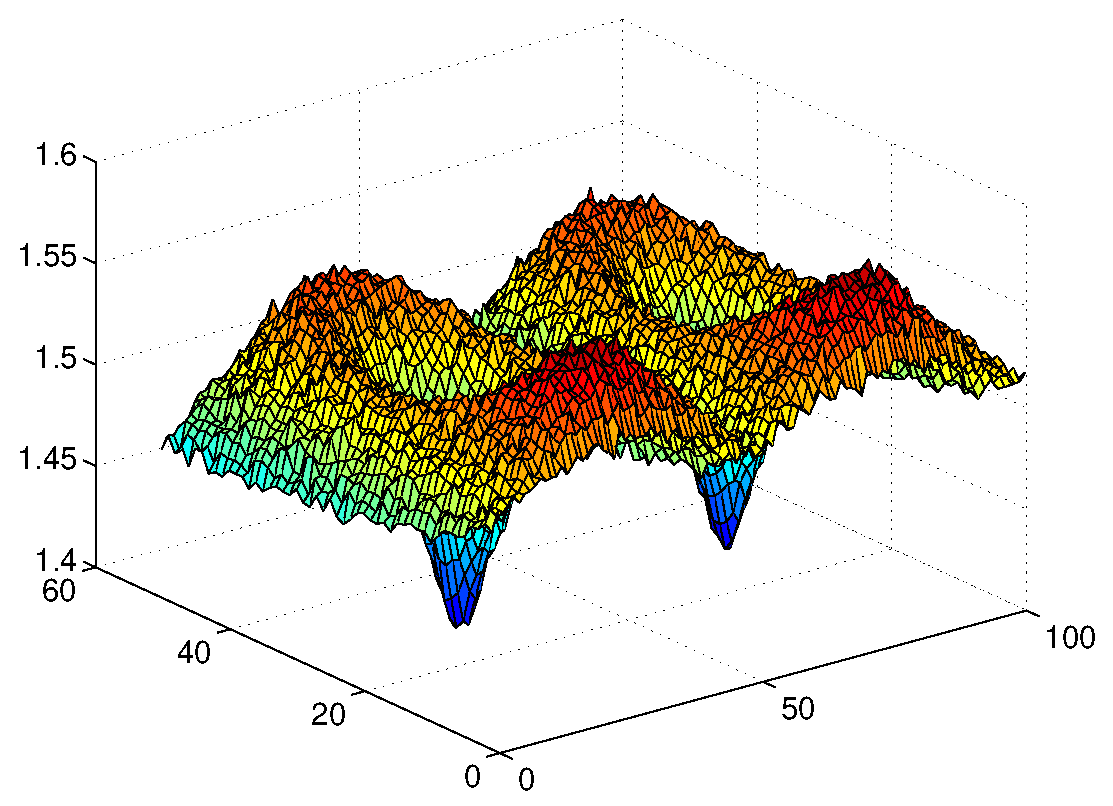
\includegraphics[width=4.5in]{figures/vanadium-surf-2.eps}
%\end{center}
%
\includegraphics[width=0.45\myheight]{risoe-logo.eps}%
%}

% The following definitions relate to the appendix on polarisation
\usepackage[dvips]{epsfig}
\usepackage{amsmath}
\parindent=0pt

\newcommand{\kappaB}{\mbox{\boldmath $\kappa$}}
\newcommand{\etaB}{\mbox{\boldmath $\eta$}}
\newcommand{\alphaB}{\mbox{\boldmath $\alpha$}}
\newcommand{\sigmaB}{\mbox{\boldmath $\sigma$}}
\newcommand{\tauB}{\mbox{\boldmath $\sigma$}}
\newcommand{\muB}{\mbox{\boldmath $\mu$}}

\def\nup{n_\uparrow}
\def\nd{n_\downarrow}

\def\Pu{P(\uparrow)}
\def\Pd{P(\downarrow)}
\def\Tu{T_\uparrow}
\def\Td{T_\downarrow}
\def\Ru{R_\uparrow}
\def\Rd{R_\downarrow}

\def\dB{\mathbf{d}}
\def\fB{\mathbf{f}}
\def\lB{\mathbf{l}}
\def\mB{\mathbf{m}}
\def\nB{\mathbf{n}}
\def\sB{\mathbf{s}}

\def\BB{\mathbf{B}}
\def\PB{\mathbf{P}}
\def\RB{\mathbf{R}}
\def\SB{\mathbf{S}}

\def\nTB{\mathbf{\tilde{n}}}

\def\Q{\mathbf{\kappaB}}
\def\tP{\mathbf{\tilde{P}}}
\def\tQ{\mathbf{\tilde{\Q}}}
\def\tN{\mathbf{\tilde{\etaB}}}
\def\FN{F_N(\Q)}
\def\FM{F_M(\Q)}
\def\ru{r_\uparrow}
\def\rd{r_\downarrow}

\def\so{\mathbf{\hat{s}}}
\def\rhoo{\hat{\rho}}
\def\betao{\hat{\beta}}
\def\alphao{\hat{\alphaB}}
\def\sigmao{\hat{\sigmaB}}
\def\sigmaH{\hat{\sigma}}
\def\muno{\mathbf{\hat{\muB}_n}}
\def\vo{\hat{V}_\BB}
\def\Io{\mathbf{\hat{I}}}

\def\madsq{|\overline{A}_d|^2}
\def\sqmad{\overline{|A_d|^2}}
\def\bd{\overline{|B_d|^2}I_d(I_d+1)}

\def\chiU{\chi_\uparrow}
\def\chiD{\chi_\downarrow}

\begin{document}

%\maketitle
% Emacs settings: -*-mode: latex; TeX-master: "manual.tex"; -*-

\begingroup                     % Make all definitions local.

%
% This was modified from risoe.sty, <2 Aug 95>
%
\catcode`\@=11
\def\@magscale#1{ scaled \magstep#1 }
\font\frtnbf = cmb10 \@magscale2
\font\twfvbf = cmbx10   \@magscale5 % extended bold
\def\maketitle{\par
 \begingroup
 \def\thefootnote{\fnsymbol{footnote}}
 \def\@makefnmark{\hbox to 0pt{$^{\@thefnmark}$\hss}}
 \if@twocolumn
 \twocolumn[\@maketitle]
 \else \newpage
 \global\@topnum\z@ \@maketitle \fi\thispagestyle{empty}\@thanks\newpage
 \endgroup
 \setcounter{footnote}{0}
 \let\maketitle\relax
 \let\@maketitle\relax
 \gdef\@thanks{}\gdef\@author{}\gdef\@title{}\let\thanks\relax}
\def\@maketitle{\newpage \baselineskip 30dd \mbox{}
 \marginpar{{\frtnbf \hfill \llap{\mbox{\reportnum \reportlan\qquad\qquad}}}}
 \par\noindent\mbox{
\includegraphics[height=1.5cm]{figures/risoe-logo.eps}\hspace{2mm}
\includegraphics[height=1.5cm]{figures/DTU_logo.ps}} \par
 \vskip 1.5cm
 {\twfvbf \noindent \@title \par} \vskip 20dd \baselineskip 16dd
 {\frtnbf\noindent\@author \par} 
 \vskip 0.5cm
 \begin{center}
     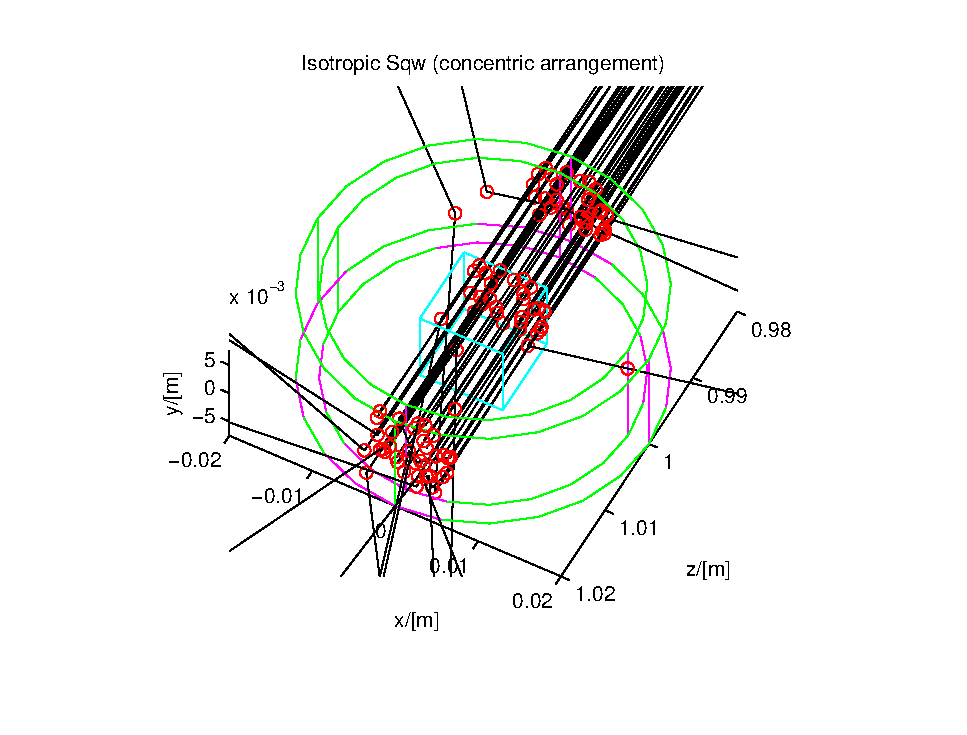
\includegraphics[width=\textwidth]{figures/sqw.eps}
   \end{center}
   \par \vfill \baselineskip 12dd
 \frtnbf\noindent Ris{\o} DTU, Roskilde, Denmark \par
 \vskip 4dd \noindent\ifcase\month\or
 January\or February\or March\or April\or May\or June\or
 July\or August\or September\or October\or November\or December\fi
 \space\number\year }

\let\reportlan=\relax
\def\month{5}                   % Released in November 2005
% Need to match front page line breaking.
\title{Component~Manual~for~\rlap{the}\\ % Avoid overfull message.
 Neutron~Ray-Tracing~Package\\
 \MCS, Version \version\ }
\author{Peter Kj\ae r Willendrup, Erik Knudsen, Kim Lefmann and\\Emmanuel Farhi}
\maketitle
\endgroup

%\begin{center}
%  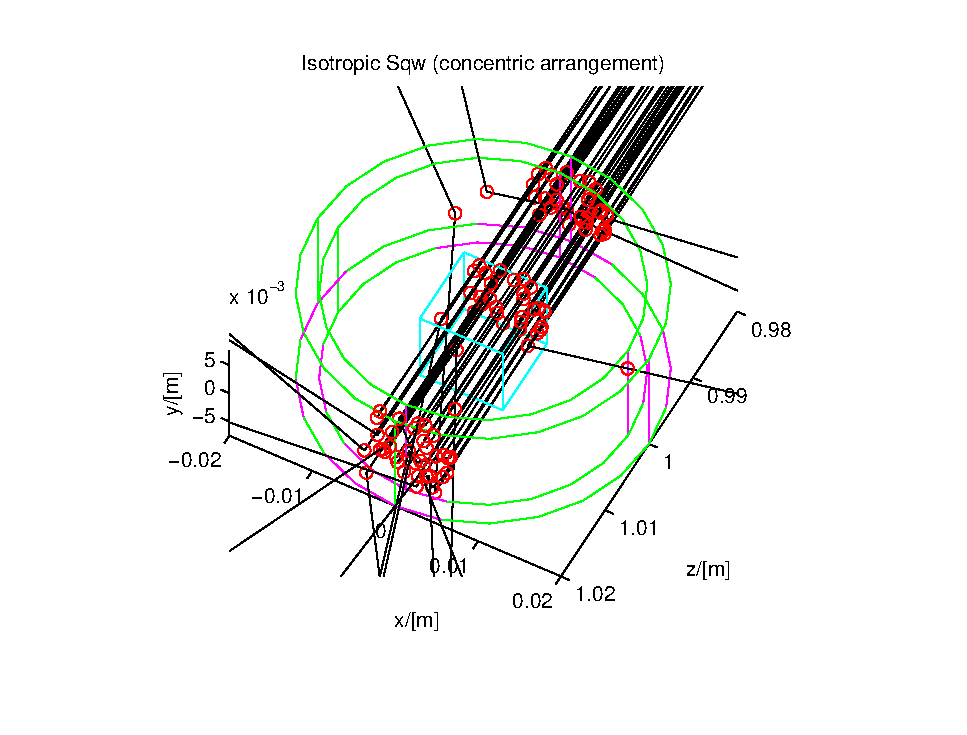
\includegraphics[width=4.5in]{figures/sqw.eps}
%\end{center}
%
% NOTE: Find a way to include this nice graphics on front page
% Currently this does not work?!?

\thispagestyle{empty}
% Emacs settings: -*-mode: latex; TeX-master: "manual.tex"; -*-

\begin{abstract}
The software package \MCX\ is a tool for carrying out Monte Carlo
ray-tracing simulations of X-ray scattering instruments with high
complexity and precision. The simulations can compute most aspects of the
performance of instruments and samples
and can thus be used to optimize the use of existing equipment,
design new instrumentation, and carry out full virtual experiments.
\MCX\ is based on a unique design where an automatic compilation process
translates high-level textual instrument descriptions into efficient
ANSI-C code. This design makes it simple to set up typical simulations
and also gives essentially unlimited freedom to handle more unusual
cases.

This report constitutes the component manual for \MCX, and,
together with the manual for the \MCX\ system, it
contains full documentation of all aspects of the program. It covers
a description of all official components of the \MCX\ package with
some theoretical background. Selected test
instruments and representative \MCX\ simulations performed with these
instruments are described in the User Manual.


\end{abstract}

\vskip\baselineskip\noindent
This report documents the components for McStas version \version,
released \reldate .
\vskip\baselineskip\noindent
The authors are:
\begin{lstlisting}
\label{p:authors}
\vskip\baselineskip\noindent
Peter Kj\ae r Willendrup \\
Materials Research Department, Ris{\o} DTU, Roskilde, Denmark \\
email: \verb+peter.willendrup@risoe.dk+
\vskip\baselineskip\noindent
Erik Knudsen \\
Materials Research Department, Ris{\o} DTU, Roskilde, Denmark \\
email: \verb+erik.knudsen@risoe.dk+
\vskip\baselineskip\noindent
Kim Lefmann \\
Niels Bohr Institute, University of Copenhagen, Denmark \\
email: \verb+lefmann@fys.ku.dk+
%\vskip\baselineskip\noindent
% Kristian Nielsen \\
% email: \verb+kristian.nielsen@mail.tele.dk+
\vskip\baselineskip\noindent
Emmanuel Farhi \\
Institut Laue-Langevin, Grenoble, France \\
email: \verb+farhi@ill.fr+
% \vskip\baselineskip\noindent
% Klaus Lieutenant \\
% Institutt for Energiteknikk, Kjeller, Norway\\
% email: \verb+Klaus.Lieutenant@ife.no+
\end{lstlisting}
%Front page illustration:\\[\baselineskip]
%Simulated scattering from a vanadium sample
%taking into account the secondary extinction. See
%section~\ref{s:vanadium-result}.
\vfill
\noindent ISBN 978--87--550--3680--2
\par\noindent ISSN 0106--2840
\par\noindent\hbox{}\hfill
    Information Service Department $\cdot$ Ris{\o} DTU $\cdot$ \number\year
%    Information Service Department $\cdot$ Ris{\o} $\cdot$ \number\year
\par
\thispagestyle{empty}\clearpage


\tableofcontents
%\pagebreak
%\listoffigures
%\pagebreak
%\listoftables

% Emacs settings: -*-mode: latex; TeX-master: "manual.tex"; -*-

\addcontentsline{toc}{chapter}{\protect\numberline{}{Preface and acknowledgements}}
\chapter*{Preface and acknowledgements}
This document contains information on the neutron scattering components
which are the building blocks for defining instruments
in the Monte Carlo neutron
ray-tracing program \MCS version \version . The initial
release in October 1998 of version 1.0 was presented in Ref.~\cite{nn_10_20}.
The reader of this
document is not supposed to have specific knowledge of neutron scattering,
but some basic understanding of physics is helpful in
understanding the theoretical background for the component functionality.
For details about setting up and running simulations, we refer to
the \MCS system manual \cite{mcstasmanual}.
We assume familiarity with the use of
the C programming language.

%We especially like to thank Kristian Nielsen for laying a solid foundation
%for the \MCS system, which the authors of this manual benefit from daily.

It is a pleasure to thank Dir.~Kurt N.~Clausen, PSI, for his continuous
support to \MCS and for having initiated the project.
Continuous support to \MCS has also come from Prof.~Robert McGreevy, ISIS.
Apart from the authors of this manual, also Per-Olof \AA strand, NTNU Trondheim,
has contributed to the development of the \MCS system.
%Both he and our other collaborators, Henrik M.\ R\o nnow and Mark
%Hagen have made major contributions to the project.  Also the
%contributions from our test users, the students Asger Abrahamsen, Niels
%Bech Christensen, and Erik Lauridsen, are gratefully acknowledged; they
%gave us an excellent opportunity to pinpoint a vast amount of serious
%errors in the test version.  Useful comments to this document itself
%have been given by Bella Lake and Alan Tennant.
We have further benefited
from discussions with many other people in the neutron scattering
community, too numerous to mention here.

%Philipp Bernhardt contributed the two chopper components in
%sections~\ref{s:chopper} and~\ref{s:first_chopper}. Emmanuel Farhi
%contributed the components in sections~\ref{s:sourceoptimizer},
%\ref{s:monitornd}, and~\ref{s:monitoroptimizer}.
The users who contributed components to this manual are acknowledged
as authors of the individual components. We encourage other
users to contribute components with manual entries for inclusion in
future versions of \MCS.

In case of errors, questions, or suggestions,
%or other need for support should arise,
do not hesitate to
contact the authors at \verb+mcstas@risoe.dk+
or consult the \MCS home page~\cite{mcstas_webpage}. A special bug/request reporting service is available \cite{mczilla_webpage}.

Important developments on the component side in \MCS version \version\
as compared to version 1.4 (the last version of the component manual;
then a section of the system manual) include

\begin{itemize}
\item{Validation of most components against analytical formula,
and benchmarking in simple cases}
\item{Newly added, realistic source components}
  \begin{itemize}
  \item \verb+ISIS_moderator+ ISIS source model based on MCNPX (D. Champion and S. Ansell, ISIS)
  \item \verb+Virtual_tripoli4_input/output+ Trioli4 (similar to MCNP) files reading/writing (G. Campioni, LLB)
  \item \verb+SNS_source+ SNS source model based on MCNPX (G. Granroth, SNS)
  \item \verb+Source_gen+ ILL sources Maxwellian parameters (E. Farhi/N. Kernavanois/H. Bordallo, ILL)
  \item \verb+ESS_moderator_short+ Calculated source model for the short pulse target station of the ESS project (K. Lefmann, Ris\o )
  \item \verb+ESS_moderator_long+ Calculated source model for the long pulse target station of the ESS project (K. Lefmann, Ris\o )
  \end{itemize}
\item{Newly added, optical components}
  \begin{itemize}
  \item \verb+Radial_collimator+ Radial collimator with both approximated and exact options (E. Farhi, ILL)
  \item \verb+FermiChopper+ and \verb+Vitess_ChopperFermi+ Two Fermi Chopper components (M. Poehlmann, G. Zsigmond, ILL and PSI)
  \item \verb+Guide_tapering+ A rectangular tapered guide (U. Filges, PSI)
  \item \verb+Guide_curved+  Non-focusing curved neutron guide (R. Stewart, ILL)
  \end{itemize}
\item{A suite of sample components}
  \begin{itemize}
  \item \verb+Inelastic_Incoherent+ Inelastic incoherent sample with quasielastic and elastic contributions (K. Lefmann, Ris\o)
  \item \verb+Phonon_simple+ An isotropic acoustic phonon (K. Lefmann, Ris\o)
  \item \verb+PowderN+. N lines powder diffraction (P.K. Willendrup, Ris\o)
  \item \verb+Sans_spheres+ hard spheres in thin solution, mono disperse (L. Arleth, the Royal Veterinary and Agricultural University (DK), K. Lefmann, Ris\o )
  \item \verb+Isotropic_Sqw+ isotropic inelastic sample (powder, liquid, glass)
elastic/inelastic scattering from $S(q,\omega)$ data (E. Farhi, V. Hugouvieux, ILL)
  \item \verb+SANS_*+ A collection of samples for SANS (H. Frielinghaus,  FZ-J\"ulich)
  \end{itemize}
\end{itemize}

We would like to kindly thank all \MCS component contributors. This is the way we improve the software alltogether.

The \MCS project has been supported by the European Union, initially
through the XENNI program and the RTD ``Cool Neutrons'' program in FP4,
In FP5, \MCS was supported strongly through the
``SCANS'' program.
Currently, in FP6, \MCS is supported through the Joint Research Activity
``MCNSI'' under the Integrated Infrastructure Initiative ``NMI3'', see
the WWW home pages~\cite{mcnsi_webpage,nmi3_webpage}.

If you {\bf appreciate} this software, please subscribe to the \verb+neutron-mc@risoe.dk+ email list, send us a smiley message, and contribute to the package. We also encourage you to refer to this software when publishing results, with the following citations:
\begin{itemize}
\item{K. Lefmann and K. Nielsen, Neutron News {\bf 10/3}, 20, (1999).}
\item{P. Willendrup, E. Farhi and K. Lefmann, Physica B, {\bf 350}, 735 (2004).}
\end{itemize}







\chapter{About the component library}
\label{c:components}
This \MCX\ Component Manual consists of the following major parts:
\begin{itemize}
\item An introduction to the use of Monte Carlo methods in \MCX .
\item A thorough description of system components,
with one chapter per major category: Sources, optics,
monochromators, samples, monitors, and other components.
\item The \MCX\ library functions and definitions
  that aid in the writing of simulations and components in
  Appendix~\ref{c:kernelcalls}.
%\item A detailed explanation of the use of random numbers
%   in Appendix~\ref{s:random}.
\item An explanation of the \MCX\ terminology in Appendix~\ref{s:terminology}.
\end{itemize}
Additionally, you may refer to the list of example instruments
from the library in the \MCX\ User Manual.

\section{Authorship}
The component library is
maintained by the \MCX\ system group. A number of basic components
``belongs'' the \MCX\ system, and are supported and tested by the \MCX\
team.

Other components are contributed
by specific authors, who are listed in the code for each component
they contribute as well as in this manual.
\MCX\ users are encouraged to send their
contributions to us for inclusion in future releases.

%Some contributed components have later been taken over
%for further development by the \MCX\ system
%group, with permission from the original authors.
%The original authors will still appear both in the component code and in the
%\MCX\ manual.

\section{Symbols for x-ray scattering and simulation}
In the description of the theory behind the component functionality
we will use the usual symbols {\bfseries r} for the position
$(x,y,z)$ of the particle (unit m), and {\bfseries k} for
the particle wave vector $(k_x, k_y, k_z)$ (unit \si{\per\angstrom}).
The wavelength is the reciprocal wave vector,
$\lambda=2 \pi / k$. By convention energy is usually given i \si{keV} and may be calculated from the wavelength by:
$\lambda=\frac{12.398}{E}$

In general, vectors are denoted by boldface symbols.

Subscripts "i" and "f" denotes ``initial'' and ``final'', respectively,
and are used in connection with the photon state before and after
an interaction with the component in question.
%This is of particular importance in sample components, where the
%wave vector change is denoted the {\em scattering vector}
%\begin{equation}\label{eq:q-transfert}
%\mathbf{ q} \equiv \mathbf{ k}_\mathrm{i} - \mathbf{ k}_\mathrm{f} .
%\end{equation}
%In analogy, the {\em energy transfer} is given by
%\begin{equation}\label{eq:w-transfert}
%\hbar \omega \equiv E_\mathrm{i}-E_\mathrm{f} =
%\frac{\hbar^2}{2 m_\mathrm{n}} \left( k_\mathrm{i}^2 - k_\mathrm{f}^2 \right).
%\end{equation}


\section{Component coordinate system}
All mentioning of component geometry refer to
the local coordinate system of the individual component.
The axis convention is so that the $z$ axis is along
the photon propagation axis, the $y$ axis is vertical up,
and the $x$ axis points left when looking along the $z$-axis,
completing a right-handed coordinate system.
Most components 'position' (as specified in the instrument description
with the \verb+AT+ keyword) corresponds to their volume centre. The mirrors
are an important counterexmaple. In this case the 'position' is the
centre of the mirror surface

Components are not necessarily designed to overlap.
This may lead to loss of rays.
Warnings will be issued during simulation if sections of the instrument
are not reached by any xrays, or if a significant number of xrays are removed.
This is usually the sign of either overlapping components
or low intensity.\index{Removed xray events}

\section{About data files}\index{Data files}\index{Library!read\_table-lib (Read\_Table)}
Some components require external data files,
e.g. lattice crystallographic definitions for Laue and powder pattern diffraction,
absorption and reflectivity files, etc.

Such files distributed with \MCX\ are located in the
\verb+data+ sub-directory of the \verb+MCXTRACE+ library.
Components that make use of the \MCX\ file system,
including the \verb+read-table+ library (see section \ref{s:read-table})
may access all \MCX\ data files without making local copies.
Of course, you are welcome to define your own data files,
and eventually contribute to \MCX\ if you find them useful.

%File extensions are not compulsory but help in identifying relevant files per
%application. We list powder and liquid data files from the \MCX\ library in
%Tables \ref{t:powders-data} and \ref{t:liquids-data}. These files contain an
%extensive header describing physical properties with references, and are
%specially suited for the PowderN (see \ref{powder}) and Isotropic\_Sqw
%components (see \ref{s:isotropic-sqw}).
%
%\begin{table}
%  \begin{center}
%    {\let\my=\\
%    \begin{tabular}{|p{0.24\textwidth}|p{0.7\textwidth}|}
%      \hline
%       \textbf{MCSTAS/data} & Description \\
%       \hline
% *.lau & Laue pattern file, as issued from Crystallographica.
%       For use with Single\_crystal, PowderN, and Isotropic\_Sqw.
%       Data: [ h   k   l Mult. d-space 2Theta   F-squared ] \\
% *.laz & Powder pattern file, as obtained from Lazy/ICSD.
%       For use with PowderN, Isotropic\_Sqw and possibly Single\_crystal.\\
% *.trm & transmission file, typically for monochromator crystals and filters.
%       Data: [ k (Angs-1) , Transmission (0-1) ] \\
% *.rfl & reflectivity file, typically for mirrors and monochromator crystals.
%       Data: [ k (Angs-1) , Reflectivity (0-1) ] \\
% *.sqw & $S(q,\omega)$ files for Isotropic\_Sqw component.
%       Data: [q] [$\omega$] [$S(q,\omega)$]\\
%      \hline
%    \end{tabular}
%    \caption{Data files of the \MCX\ library.}
%    \label{t:comp-data}
%    \index{Library!Components!data}
%    }
%  \end{center}
%\end{table}
%
%\begin{table}
%  \begin{center}
%    {\let\my=\\
%    \begin{small}
%    \begin{tabular}{|l|rrr|rr|p{0.2\textwidth}|}
%
%      \hline
%      \textbf{ MCSTAS/data} & $\sigma_{coh}$&$\sigma_{inc}$&$\sigma_{abs}$&$T_m$       & $c$    & Note \\
%          File name     & [barns]     & [barns]    & [barns]    & [K]        & [m/s] & \\
%      \hline
%Ag.laz             & 4.407     & 0.58     &{\bfseries 63.3}      &1234.9    &2600&\\
%Al2O3\_sapphire.laz & 15.683    & 0.0188   &0.4625    &2273      &   &\\
%Al.laz             & 1.495     & 0.0082   &0.231     &933.5     &5100& .lau\\
%Au.laz             & 7.32      & 0.43     &{\bfseries 98.65}     &1337.4    &{\bfseries 1740}&\\
%B4C.laz            & 19.71     & 6.801    &{\bfseries 3068}      &2718      &     &\\
%Ba.laz             & 3.23      & 0.15     &29.0      &1000      &{\bfseries 1620}&\\
%Be.laz             & 7.63      & 0.0018   &0.0076    &1560      &13000&\\
%BeO.laz            & 11.85     & 0.003    &0.008     &2650      &   & .lau\\
%Bi.laz             & 9.148     & 0.0084   &0.0338    &544.5     &{\bfseries 1790}&\\
%C60.lau            & 5.551     & 0.001    &0.0035    &          &   &\\
%C\_diamond.laz      & 5.551     & 0.001    &0.0035    &4400      &18350 & .lau\\
%C\_graphite.laz     & 5.551     & 0.001    &0.0035    &3800      &18350 & .lau\\
%Cd.laz             & 3.04      & 3.46     &{\bfseries 2520}      &594.2     &2310&\\
%Cr.laz             & 1.660     & 1.83     &3.05      &2180      &5940&\\
%Cs.laz             & 3.69      & 0.21     &29.0      &301.6     &{\bfseries 1090}  & $c$ in liquid\\
%Cu.laz             & 7.485     & 0.55     &3.78      &1357.8    &3570&\\
%Fe.laz             & 11.22     & 0.4      &2.56      &1811      &4910&\\
%Ga.laz             & 6.675     & 0.16     &2.75      &302.91    &2740&\\
%Gd.laz             & 29.3      & 151      &{\bfseries 49700}     &1585      &2680&\\
%Ge.laz             & 8.42      & 0.18     &2.2       &1211.4    &5400  & \\
%H2O\_ice\_1h.laz     & 7.75      & 160.52   &0.6652    &273       &     &\\
%Hg.laz             & 20.24     & 6.6      &{\bfseries 372.3}     &234.32    &{\bfseries 1407}&\\
%I2.laz             & 7.0       & 0.62     &12.3      &386.85    &   &\\
%In.laz             & 2.08      & 0.54     &{\bfseries 193.8}     &429.75    &{\bfseries 1215}&\\
%K.laz              & .69       & 0.27     &2.1       &336.53    &{\bfseries 2000}&\\
%LiF.laz            & 4.46      & 0.921    &{\bfseries 70.51}     &1140      &   &\\
%Li.laz             & 0.454     & 0.92     &{\bfseries 70.5}      &453.69    &6000&\\
%Nb.laz             & 8.57      & 0.0024   &1.15      &2750      &3480&\\
%Ni.laz             & 13.3      & 5.2      &4.49      &1728      &4970&\\
%Pb.laz             & 11.115    & 0.003    &0.171     &600.61    &{\bfseries 1260}&\\
%Pd.laz             & 4.39      & 0.093    &6.9       &1828.05   &3070&\\
%Pt.laz             & 11.58     & 0.13     &10.3      &2041.4    &2680&\\
%Rb.laz             & 6.32      & 0.5      &0.38      &312.46    &{\bfseries 1300}  & \\
%Se\_alpha.laz       & 7.98      & 0.32     &11.7      &494       &3350&\\
%Se\_beta.laz        & 7.98      & 0.32     &11.7      &494       &3350&\\
%Si.laz             & 2.163     & 0.004    &0.171     &1687      &2200&\\
%SiO2\_quartza.laz   & 10.625    & 0.0056   &0.1714    &846       &      & .lau\\
%SiO2\_quartzb.laz   & 10.625    & 0.0056   &0.1714    &1140      &      & .lau\\
%Sn\_alpha.laz       & 4.871     & 0.022    &0.626     &505.08    &     &\\
%Sn\_beta.laz        & 4.871     & 0.022    &0.626     &505.08    &2500&\\
%Ti.laz             & 1.485     & 2.87     &6.09      &1941      &4140&\\
%Tl.laz             & 9.678     & 0.21     &3.43      &577       &{\bfseries 818}&\\
%V.laz              & .0184     & 4.935    &5.08      &2183      &4560&\\
%Zn.laz             & 4.054     & 0.077    &1.11      &692.68    &3700&\\
%Zr.laz             & 6.44      & 0.02     &0.185     &2128      &3800&\\
%      \hline
%    \end{tabular}\end{small}
%    \caption{Powders of the \MCX\ library \cite{icsd_ill,ILLblue}. Low $c$ and high $\sigma_{abs}$ materials are highlighted. Files are given in LAZY format, but may exist as well in Crystallographica \textit{.lau} format as well.}
%    \label{t:powders-data}
%    \index{Library!Components!data}
%    }
%  \end{center}
%\end{table}
%
%\begin{table}
%  \begin{center}
%    {\let\my=\\
%    \begin{small}
%    \begin{tabular}{|l|rrr|rr|p{0.2\textwidth}|}
%
%      \hline
%      {\bfseries MCSTAS/data} & $\sigma_{coh}$&$\sigma_{inc}$&$\sigma_{abs}$&$T_m$       & $c$    & Note \\
%          File name     & [barns]     & [barns]    & [barns]    & [K]        & [m/s] & \\
%      \hline
%Cs\_liq\_tot.sqw                      & 3.69      & 0.21     &29.0      &301.6     &{\bfseries 1090}  & Measured \\
%Ge\_liq\_coh.sqw and Ge\_liq\_inc.sqw & 8.42      & 0.18     &2.2       &1211.4    &5400  & Ab-initio MD \\
%He4\_liq\_coh.sqw                     & 1.34      & 0        &0.00747   &0         &{\bfseries 240}   & Measured\\
%Ne\_liq\_tot.sqw                      & 2.62      & 0.008    &0.039     &24.56     &{\bfseries 591}   & Measured\\
%Rb\_liq\_coh.sqw and Rb\_liq\_inc.sqw & 6.32      & 0.5      &0.38      &312.46    &{\bfseries 1300}  & Classical MD \\
%Rb\_liq\_tot.sqw                      & 6.32      & 0.5      &0.38      &312.46    &{\bfseries 1300}  & Measured \\
%      \hline
%    \end{tabular}\end{small}
%    \caption{Liquids of the \MCX\ library \cite{icsd_ill,ILLblue}. Low $c$ and high $\sigma_{abs}$ materials are highlighted.}
%    \label{t:liquids-data}
%    \index{Library!Components!data}
%    }
%  \end{center}
%\end{table}

\MCX\ itself generates both simulation and monitor data files, the structure of which is explained in the User Manual (see end of chapter 'Running \MCX').

\section{Component source code}
Source code for all components may be found in the \verb+MCXTRACE+ library
subdirectory of the McXtrace installation;
the default is \verb+/usr/local/lib/mcxtrace/+
on Unix-like systems and \verb+C:\mcxtrace\lib+ on Windows systems, but it may be
changed using the \verb+MCXTRACE+ environment variable.
\index{Environment variable!MCXTRACE}

In case users only require to add new features, preserving the existing features of a component, 
using the \verb+EXTEND+ keyword\index{Keyword!EXTEND} in the instrument description file is recommended. For larger modification of a component, it is advised to make a copy
of the component file into the working directory.
A component file in the local directory will in \MCX takes precedence over
a library component of the same name.

\section{Documentation}
As a complement to this Component Manual, we encourage users to use
the \verb+mxdoc+ front-end which enables to display both the
catalog of the \MCX\ library, e.g using: \index{Tools!mcdoc}
\begin{quote}
  \verb|mxdoc|
\end{quote}
as well as the documentation of specific components, e.g with:
\begin{quote}
  \verb|mxdoc --text| \textit{name} \\
  \verb|mxdoc| \textit{file.comp}
\end{quote}
The first line will search for all components matching the \textit{name},
and display their help section as text. For instance, \verb+mxdoc .laz+ will list all available Lazy data files, whereas \verb+mxdoc --text Monitor+ will list most Monitors.
The second example will display the help corresponding to
the \textit{file.comp} component, using your
BROWSER\index{Environment variable!BROWSER} setting, or as text if unset.
The \verb+--help+ option will display the command help, as usual.

An overview of the component library is also given at the \MCX home page \cite{mcxtrace_webpage} and in the User Manual \cite{mcxtracemanual}.

\section{Disclaimer, bugs}\index{Bugs}

We would like to emphasize that the usage of both the \MCX software, as well as
its components are the responsability of the users. Indeed, obtaining accurate
and reliable results requires a substantial work when writing instrument
descriptions. This also means that users should read carefully both the
documentation from the manuals \cite{mcxtracemanual} and from the component
itself (using \verb+mcdoc+ \textit{comp}) before reporting errors. Most
anomalous results often originate from a wrong usage of some part of the
package.

Anyway, if you find that either the documentation is not clear, or the behavior
of the simulation is undoubtedly anomalous, you should report this to us at
\verb+mcxtrace-users@mcxtrace.org+ and/or refer to our special bug/request reporting service
\cite{mczilla_webpage}.

\chapter{Monte Carlo Techniques and simulation strategy}
\label{s:MCtechniques}\index{Monte Carlo method}

This chapter explains the simulation strategy and the Monte Carlo
techniques used in \MCS. We first explain the concept of the neutron
weight factor, and discuss the statistical errors in dealing with sums
of neutron weights.  Secondly, we give an expression for how the weight
factor transforms under a Monte Carlo choice and specialize this
to the concept of direction focusing.  Finally, we present a way of
generating random numbers with arbitrary distributions.
More details are available in the Appendix concerning random numbers in the User manual.


\section{Neutron spectrometer simulations}

Neutron scattering instruments are built as a series of neutron optics elements. Each of these elements modifies the beam characteristics (e.g. divergence, wavelength spread, spatial and time distributions) in a way which, for simple neutron beam configurations, may be modelled with analytical methods. This is valid for individual elements such as guides \cite{Leibnitz63,Mildner90}, choppers \cite{Lowde60,Copley03}, Fermi choppers \cite{Fermi47,Peters05}, velocity selectors \cite{Clark66}, monochromators \cite{Freund83,Sears97,Shirane02,Alianelli04}, and detectors \cite{Radeka74,Charpak89,Manzin04}. In the case of a limited number of optical elements, the so-called acceptance diagram theory \cite{Mildner90,Copley93,Cussen03} may be used, within which the neutron beam distributions are considered to be homogeneous, triangular or Gaussian.
However, real neutron instruments are constituted of a large number of optical elements, and this brings additional complexity by introducing strong correlations between neutron beam parameters like divergence and position - which is the basis of the acceptance diagram method - but also wavelength and time. The usual analytical methods, such as phase-space theory, then reach their limit of validity in the description of the resulting effects.

In order to cope with this difficulty, Monte Carlo (MC) methods (for a general review, see Ref. \cite{James80}) may be applied to the simulation of neutron instruments.
The use of probability is common place in the description of microscopic physical processes. Integrating these events (absorption, scattering, reflection, ...) over the neutron trajectories
results in an estimation of measurable quantities characterizing the neutron instrument. Moreover, using variance reduction (importance sampling)
where possible, reduces the computation time and gives better accuracy.

Early implementations of the MC method for neutron instruments used \emph{home-made} computer programs  (see \cite{Copley86,Mildner77}) but, more recently, general packages have been designed, providing models for most optical components of neutron spectrometers.
The most widely-used packages are NISP \cite{NISP}, ResTrax \cite{Restrax}, McStas \cite{nn_10_20,mcstas_webpage}, Vitess \cite{Vitess}, and IDEAS \cite{IDEAS}, which allow a wide range of neutron scattering instruments to be simulated.

The neutron ray-tracing Monte Carlo method has been used widely for guide studies \cite{Copley93,Farhi02,Schanzer04}, instrument optimisation and design \cite{Zsigmond04,Lieutenant05}. Most of the time, the conclusions and general behaviour of such studies may be obtained using the classical analytical approaches, but accurate estimates for the flux, resolution and generally the optimum parameter set, benefit considerably from MC methods.

\subsection{Monte Carlo ray tracing simulations}
Mathematically, the Monte-Carlo method is an application of the law of large numbers \cite{James80,Grimmett92}. Let $f(u)$ be a finite continuous integrable function of parameter $u$ for which an integral estimate is desirable. The discrete statistical mean value of $f$ (computed as a series) in the uniformly sampled interval $a < u < b$ converges to the mathematical mean value of $f$ over the same interval.

\begin{equation}
\lim_{n \rightarrow \infty} \frac{1}{n} \sum_{i=1, a \leq u_i \leq b}^n f(u_i) = \frac{1}{b-a}\int_a^b f(u) du
\end{equation}

In the case were the $u_i$ values are regularly sampled, we come to the well known midpoint integration rule. In the case were the $u_i$ values are randomly (but uniformly) sampled, this is the Monte-Carlo integration technique. As random generators are not perfect, we rather talk about \emph{quasi}-Monte-Carlo technique. We encourage the reader to refer to James \cite{James80} for a detailed review on the Monte-Carlo method.

\section{The neutron weight}
\label{s:probweight}
A totally realistic semi-classical simulation will require that
each neutron is at any time either present or lost.
In many instruments, only a very
small fraction of the initial neutrons will ever be detected, and
simulations of this kind will therefore waste much time in dealing
with neutrons that never hit the detector.

An important way of speeding up calculations is to introduce
a neutron "weight factor" for each simulated neutron ray and to
adjust this weight according to the path of the ray.
If {\em e.g.}\ the reflectivity of a certain
optical component is 10\%, and only reflected neutrons ray are
considered later in the simulations, the neutron
weight will be multiplied by 0.10 when passing this component,
but every neutron is allowed to reflect in the component.
In contrast, the totally realistic simulation of the component
would require in average ten incoming neutrons for each reflected one.

Let the initial neutron weight be $p_0$ and let us denote the weight
multiplication factor in the $j$'th component by $\pi_j$.  The resulting
weight factor for the neutron ray after passage of the whole instrument
becomes the product of all contributions
\begin{equation}
\label{e:probprod}
p = p_n = p_0 \prod_{j=1}^n \pi_j .
\end{equation}
Each adjustement factor should be $0 < \pi_j < 1$, except in special circumstances, so that total flux can only decrease through the simulation. For convenience, the value of $p$ is updated (within each component)
during the simulation.

Simulation by weight adjustment is performed
whenever possible. This includes
\begin{itemize}
\item Transmission through filters and windows.
\item Transmission through Soller blade collimators and velocity
  selectors
 (in the approximation
 which does not take each blade into account).
\item Reflection from monochromator (and analyser) crystals
 with finite reflectivity and mosaicity.
\item Reflection from guide walls.
\item Passage of a continuous beam through a chopper.
\item Scattering from all types of samples.
\end{itemize}

\subsection{Statistical errors of non-integer counts}
\label{s:staterror}

In a typical simulation, the result will consist of a
count of neutrons histories ("rays") with different weights. The
sum of these weights is an estimate of the mean number of neutrons
hitting the monitor (or detector) per second in a ``real'' experiment.
One may write the counting result as
\begin{equation}
\label{psum}
I = \sum_i p_i = N \overline{p} ,
\end{equation}
where $N$ is the number of rays hitting the detector and the horizontal bar
denotes averaging.
By performing the weight transformations, the (statistical)
mean value of $I$ is unchanged. However, $N$ will in general be enhanced,
and this will improve the accuracy of the simulation.

To give an estimate of the statistical error, we proceed as follows:
Let us first for simplicity assume that all the counted neutron weights are
almost equal, $p_i \approx \overline{p}$,
and that we observe a large number of neutrons, $N \geq 10$.
Then $N$ almost follows a normal distribution
with the uncertainty $\sigma(N) = \sqrt{N}$
\footnote{This is not correct in a
situation where the detector counts a large fraction of the
neutrons in the simulation, but we will neglect that for now.}.
Hence, the statistical uncertainty of the observed intensity becomes
\begin{equation} \label{e:sigI1}
 \sigma(I) = \sqrt{N} \overline{p} = I / \sqrt{N} ,
\end{equation}
as is used in real neutron experiments (where $\overline{p} \equiv 1$).
For a better approximation we return to Eq.~(\ref{psum}).
Allowing variations in both $N$ and $\overline{p}$,
we calculate the variance of the resulting intensity,
assuming that the two variables are independent:
\begin{equation}
\sigma^2(I) = \sigma^2(N) \overline{p}^2 + N^2 \sigma^2(\overline{p}) .
\end{equation}
Assuming as before that $N$ follows a normal distribution, we reach
$\sigma^2(N) \overline{p}^2 = N \overline{p}^2$.
Further, assuming that the individual weights, $p_i$,
follow a Gaussian distribution (which in some cases is far from the truth)
we have
$N^2 \sigma^2(\overline{p}) = \sigma^2(\sum_i p_i) = N \sigma^2(p_i)$
and reach
\begin{equation}
\sigma^2(I) = N \left( \overline{p}^2 + \sigma^2(p_i) \right).
\end{equation}
The statistical variance of the $p_i$'s is estimated by
$\sigma^2(p_i) \approx  (\sum_i p_i^2 - N \overline{p}^2) / (N-1)$.
The resulting variance then reads
\begin{equation}
\sigma^2(I) = \frac{N}{N-1} \left( \sum_i p_i^2 - \overline{p}^2  \right) .
\end{equation}
For almost any positive value of $N$, this is very well approximated
by the simple expression
\begin{equation}
\sigma^2(I) \approx \sum_i p_i^2 .
\end{equation}
As a consistency check, we note that for all $p_i$ equal, this reduces to
eq.~(\ref{e:sigI1})

In order to compute the intensities and uncertainties, the detector components
in \MCS\ will keep track of
$N=\sum_i p_i^0, I=\sum_i p_i^1$, and $M_2 = \sum_i p_i^2$.

\section{Weight factor transformations during a Monte Carlo
 choice}
When a Monte Carlo choice must be performed, {\em e.g.} when the
initial energy and direction of the neutron ray is decided at the source,
it is important to adjust the neutron weight so that the combined
effect of neutron weight change and Monte Carlo probability
of making this particular choice
equals the actual physical properties we like to model.

Let us follow up on the simple example of transmission.
The probability of transmitting the real neutron is $P$, but we make
the Monte Carlo choice of transmitting the neutron ray each time:
$f_{\rm MC}=1$. This must be reflected on the choice of weight multiplier
$\pi_j$ given by the master equation
%In the ``real'' semi-classical world, there is a distribution
%(probability density) for the neutrons in the six dimensional
%(energy, direction, position) space of
%$\Pi(E,\Ombold,{\bf r}) = dP/(dE d\Ombold d^3{\bf r})$ depending upon
%the source temperature, geometry {\em etc.}\ In the
%Monte Carlo simulations, the six coordinates are for efficiency reasons
%in general picked from another distribution:
%$f_{\rm MC}(E,\Ombold,{\bf r}) \neq \Pi(E, \Ombold,{\bf r})$,
%since one would {\em e.g.} often generate
%only neutrons within a certain parameter interval.
%However, we must then require that the weights are adjusted
%by a factor $\pi_j$ (in this case: $j=1$) so that
\begin{equation} \label{probrule}
f_{\rm MC} \pi_j = P .
\end{equation}
%For the sources present in version \version,
%only the $(\Ombold, {\bf r})$ dependence of the correction factors
%are taken into account.

This probability rule is general, and holds also if, e.g., it is decided to
transmit only half of the rays $(f_{\rm MC}=0.5)$.
An important different example
is elastic scattering from a powder sample,
where the Monte-Carlo choices are the particular powder line to scatter from,
the scattering position within the sample and the final neutron direction
within the Debye-Scherrer cone.

\subsection{Direction focusing}
\index{Monte Carlo method!Direction focusing}
\label{s:focus}
An important application of weight transformation is direction focusing.
Assume that the sample scatters the neutron rays in many directions.
In general, only neutron rays in some of these directions will
stand any chance of being detected. These directions we call
the {\em interesting directions}.
The idea in focusing is to avoid wasting computation time on
neutrons scattered in the other directions.
This trick is an instance of what in Monte Carlo terminology
is known as {\em importance sampling}. % \cite{importance}.

If {\em e.g.} a sample scatters isotropically
over the whole $4\pi$ solid angle, and all interesting
directions are known to be contained within a certain
solid angle interval $\Delta \Ombold$, only these solid angles
are used for the Monte Carlo choice of scattering direction.
According to Eq.~(\ref{probrule}), the weight factor will then have
to be changed by the amount
$\pi_j = |\Delta \Ombold| / (4 \pi)$.
One thus ensures that the mean simulated intensity is unchanged
during a "correct" direction focusing, while a too narrow focusing will
result in a lower (\textit{i.e.} wrong) intensity, since
we cut neutrons rays that should have reached the final detector.

\begin{figure}[htb!]
\begin{center}
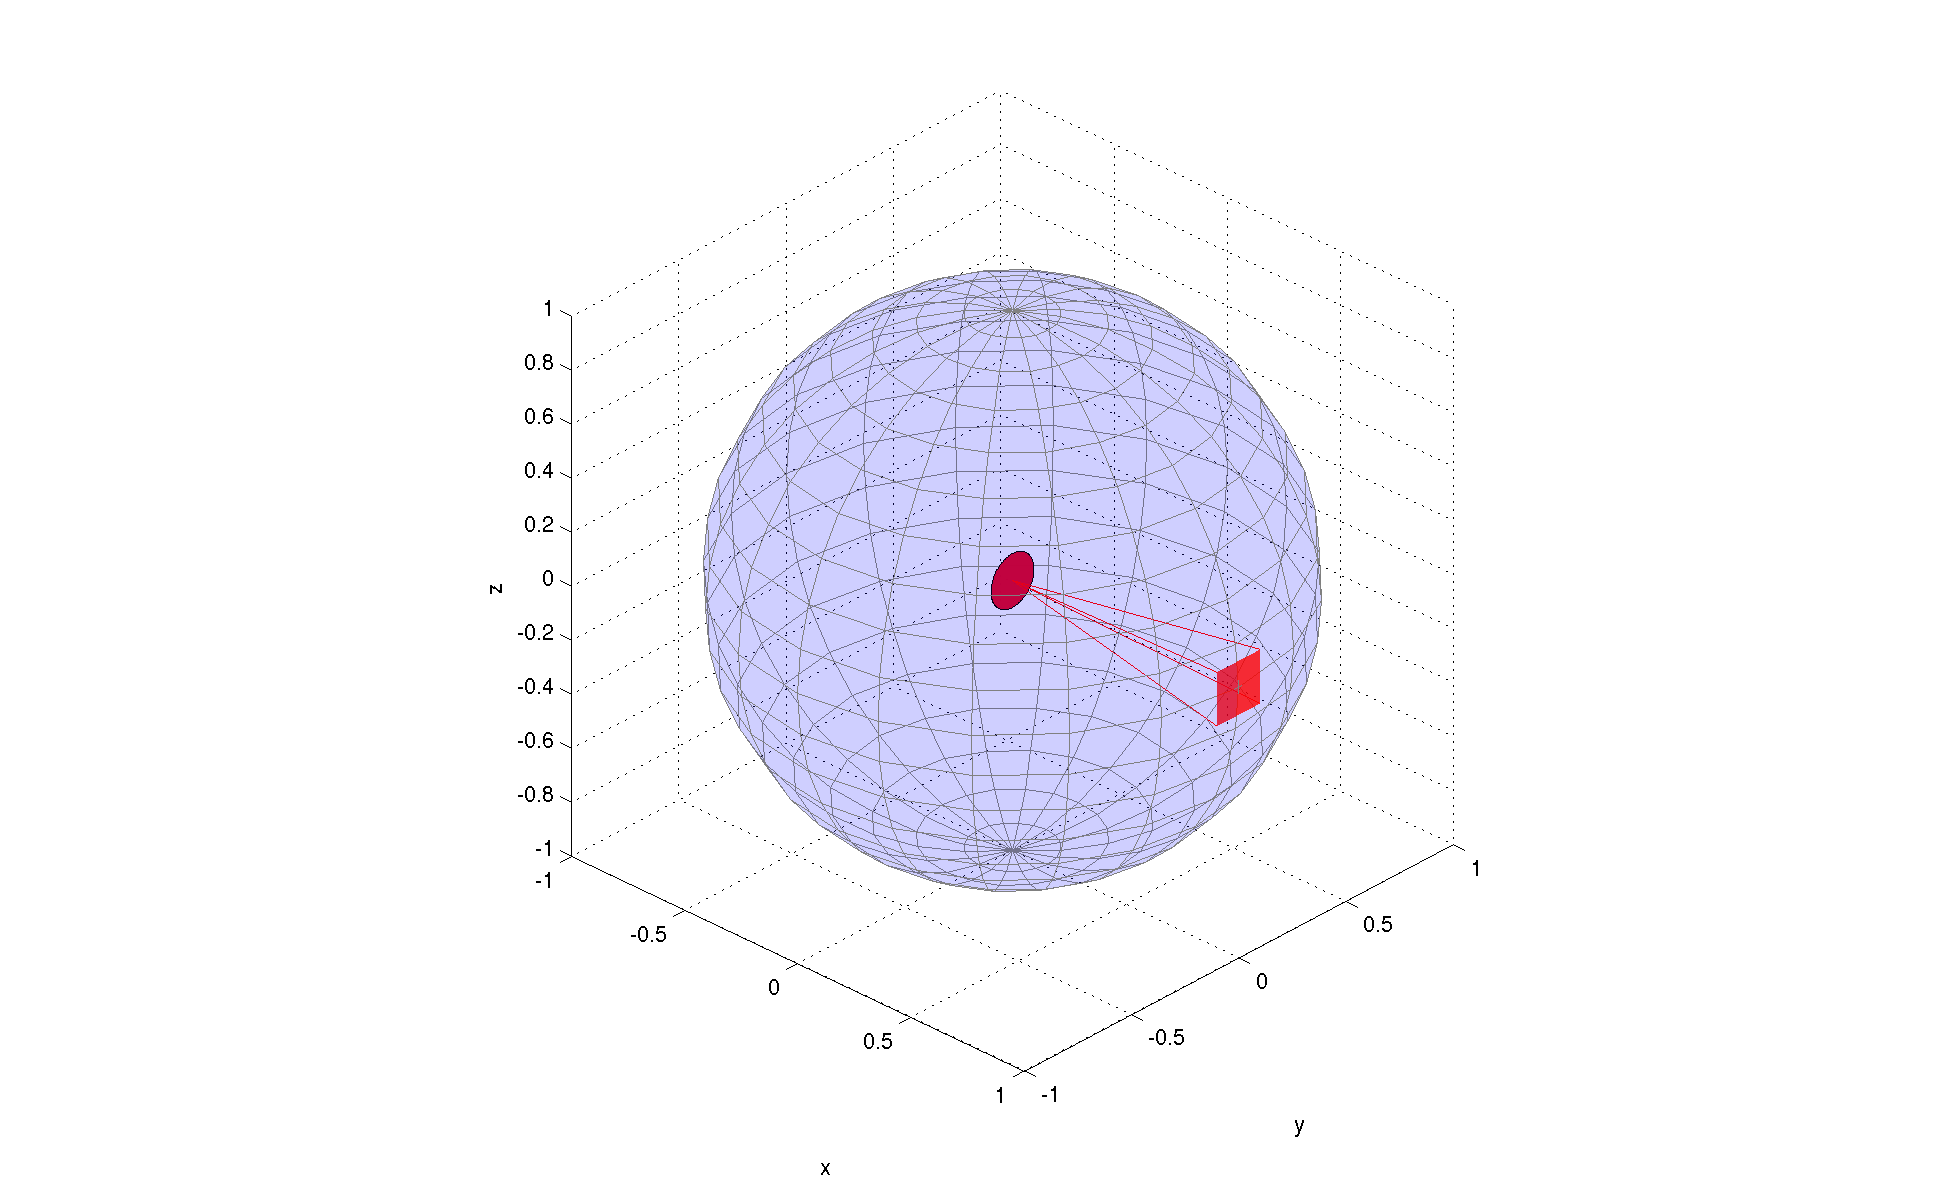
\includegraphics[width=.8\textwidth]{figures/focusing}
\end{center}
\caption{Illustration of the effect of direction focusing in \MCS\
  . Weights of neutrons emitted into a certain solid angle are
  scaled down by the full unit sphere area.}
\label{fig:focusing}
\end{figure}

\section{Adaptive and Stratified sampling}
\index{Monte Carlo method!Adaptive sampling}
\index{Monte Carlo method!Stratified sampling}
Another strategy to improve sampling in simulations
is \emph{adaptive importance sampling} (also called variance reduction technique), % \cite{importance},
where \MCS\ during the simulations will determine
the most interesting directions and gradually change
the focusing according to that.
Implementation of this idea is
found in the {\bf Source\_adapt} and {\bf Source\_Optimizer} components.
%, described in section~\ref{s:Source_adapt}.

An other class of efficiency improvement technique is the so-called \emph{stratified sampling}. It consists in partitioning the event distributions in representative sub-spaces, which are then all sampled individualy. The advantage is that we are then sure that each sub-space is well represented in the final integrals. This means that instead of shooting $N$ events, we define $D$ partitions and shoot $r=N/D$ events in each partition. In conjunction with adaptive sampling, we may define partitions so that they represent 'interesting' distributions, e.g. from events scattered on a monochromator or a sample. The sum of partitions should equal the total space integrated by the Monte Carlo method, and each partition must be sampled randomly.

In the case of \MCS, the stratified sampling is used when repeating events, such as in the Virtual sources (Virtual\_input, Vitess\_input, Virtual\_mcnp\_input, Virtual\_tripoli4\_input) and when using the SPLIT keyword in the TRACE section on instrument descriptions. We emphasize here that the number of repetitions $r$ should not exceed the dimensionality of the Monte Carlo integration space (which is $d=10$ for neutron events) and the dimensionality of the partition spaces, i.e. the number of random generators following the stratified sampling location in the instrument.

\section{Accuracy of Monte Carlo simulations}
\index{Monte Carlo method!Accuracy}

When running a Monte Carlo, the meaningfull quantities are obtained by integrating random events into a single value (e.g. flux), or onto an histogram grid. The theory \cite{James80} shows that the accuracy of these estimates is a function of the space dimension $d$ and the number of events $N$. For large numbers $N$, the central limit theorem provides an estimate of the relative error as $1/\sqrt{N}$. However, the exact expression depends on the random distributions.

\MCS\ uses a space with $d=10$ parameters to describe neutrons (position, velocity, spin, time). We show in Table \ref{t:mc_accuracy} a rough estimate of the accurarcy on integrals as a function of the number of records reaching the integration point. This stands both for integrated flux, as well as for histogram bins - for which the number of events per bin should be used for $N$.

\begin{table}
  \begin{center}
  {\let\my=\\
    \begin{tabular}{|c|c|}
    \hline
    Records       & Accurarcy \\
    \hline
    $10^3$ & 10 \% \\
    $10^4$ & 2.5 \% \\
    $10^5$ & 1 \% \\
    $10^6$ & 0.25 \% \\
    $10^7$ & 0.05 \% \\
    \hline
    \end{tabular}
    \caption{Accuracy estimate as a function of the number of statistical events used to estimate an integral with \MCS.}
    \label{t:mc_accuracy}
  }
  \end{center}
\end{table}


% Emacs settings: -*-mode: latex; TeX-master: "manual.tex"; -*-

\chapter{Source components}
\label{c:source}
\index{Sources|textbf}
\index{Library!Components!sources}

\MCX\ contains a number of different source components,
and any simulation will usually contain exactly one of these sources.
The main function of a source is to determine a set of initial
parameters $(\mathbf{r}, \mathbf{v}, t)$
for each neutron ray. This is done by Monte Carlo choices from
suitable distributions. For example, in most present sources
the initial position is
found from a uniform distribution over the source surface,
which can be chosen to be either circular or rectangular.
The initial neutron velocity is selected within an interval
of either the corresponding energy or the corresponding wavelength.
Polarization is not relevant for sources,
and we initialize the neutron average spin to zero: $\mathbf{s}=(0,0,0)$.

For time-of-flight sources, the choice of the emission time, $t$,
is being made on basis of detailed analytical expressions.
For other sources, $t$ is set to zero.
In the case one would like to use a steady state source
with time-of-flight settings,
the emission time of each neutron ray should be determined using
a Monte Carlo choice. This may be achieved by
the \verb+EXTEND+ keyword in the instrument description source
as in the example below:\index{Keyword!EXTEND}

\begin{verbatim}
  TRACE

  COMPONENT MySource=Source_gen(...) AT (...)
  EXTEND
  %{
    t = 1e-3*randpm1(); /* set time to +/- 1 ms */
  %}
\end{verbatim}

\subsection{Photon flux and Brilliance}
\label{s:xray-flux}
The flux of the sources deserves special attention. The total
intensity is defined as the sum of weights of all emitted xrays
during one simulation
(the unit of total photon weight is thus xrays per second).
The flux, $\psi$, at an instrument is defined as intensity per area perpendicular
to the beam direction.

The source flux, $\Phi$, is defined in different units:
the number of photon rays emitted per second from a
1~cm$^2$ area on the source surface,
with direction within a 1~ster.\ solid angle,
and with wavelength within a 1 {\AA} interval.
The total intensity of real neutrons emitted towards a given diaphragm
(units: n/sec) is therefore (for constant $\Phi$):
\begin{equation}
I_\mathrm{total} = \Phi A \Delta\Omega \Delta\lambda ,
\end{equation}
where $A$ is the source area, $\Delta\Omega$ is the solid angle of the
diaphragm as seen from the source surface, and $\Delta\lambda$ is the
width of the wavelength interval in which neutrons are emitted (assuming
a uniform wavelength spectrum).

The simulations are performed so that detector intensities
are independent of the number of neutron histories simulated
(although more neutron histories will give better statistics).
If $N_\mathrm{sim}$ denotes the number of
xray histories to simulate, the initial photon weight $p_0$ must be set to
\begin{equation}
\label{proprule}
p_0 = \frac{N_\mathrm{total}}{N_\mathrm{sim}} =
    \frac{\Phi(\lambda)}{N_\mathrm{sim}} A \Omega \Delta\lambda ,
\end{equation}
where the source flux is now given a $\lambda$-dependence.

As a start, we recommend new \MCX\ users to use the
\textbf{Source\_simple} component.
Slightly more realistic sources are \textbf{Source\_Maxwell\_3} for
continuous sources or \textbf{Moderator} for time-of-flight sources.

Optimizers can dramatically improve the statistics, but may occasionally
give wrong results, due to misleaded optimization.
You should always check such simulations with (shorter) non-optimized ones.

Other ways to speed-up simulations are to read events from a file.
See section \ref{sources-seealso} for details.

\begin{figure}
  \begin{center}
    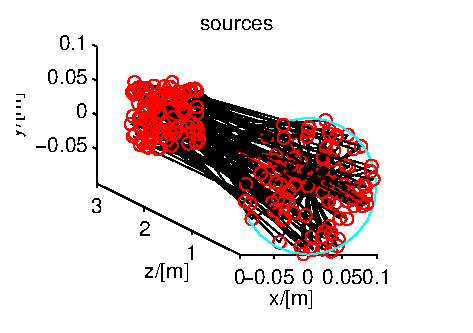
\includegraphics[width=0.75\textwidth]{figures/sources.eps}
  \end{center}
\caption{A circular source component (at z=0) emitting photon rays randomly, either from a model, or from a data file.}
\label{f:source}
\end{figure}

\newpage
\section{Source\_pt: A mathematical point emitting photons with a spectrum either uniform, gaussian or generated from a datafile}
\label{source-pt}
\index{Sources!Point source}
\component{Source\_pt}{System}{$dist$,$focus\_xw$,$focus\_yh$}{$\lambda_0$,${\rm d}\lambda$,$E$, $dE$, $spectrum\_file$, $incoherent$,$phase$}

The simplest source model, where a mathematical point source at $(0,0,0)$ emits photons. The wavevector of the emitted photons
is picked randomly in a defining aperture $focus\_xw$ by $focus\_yh$ m at $(0,0,dist)$. 
Please note that this aperture is merely a
virtual aperture used to reduce the sampling space. This has a few
implications: Other components may be placed without reference to the aperture,
but if the aperture does not fill the full acceptance window of subsequent
components your simulations will be biased. The aperture is simply there to provide efficient sampling.

If a $spectrum\_file$ is not supplied, the xray
is given a weight which is the total wavelength-integrated intensity downscaled
by the
solid subtended by the definning aperture.

If a $spectrum\_file$ \emph{is} supplied, a slightly different strategy is adopted. In this case the
wavelength/energy range implied by the datafile is sampled unformly and each ray is assigned
a weight corresponding to the intensity indicated by linear interpolation between datapoints
at that wavelength. This implies an oversampling of weak parts of the intensity spectrum.

Currently only completely coherent or fully incoherent beams are supported. If
$phase$ is specified emitted photons be assigne dthat phase, otherwise it is
chosen randomly.


\section{Source\_flat: A flat surface emitting photons with a spectrum either uniform, gaussian or generated from a datafile}
\label{source-flat}
\index{Sources!Flat surface source}
\component{Source\_flat}{System}{$d$,$w$,$h$}{$r$,$x_{width}$,$y_{height}$,$d$, $\lambda_0$,${\rm d}\lambda$, $spectrum\_file$, $incoherent$,$phase$}

A simple source model, with a flat surface emitting photons. The surface in the
$xy$-plane is specified as a rectangle with dimensions
$x_{width}\times y_{height}$ m, or as a circle w radius,$r$. 
The initial xray position is chosen randomly in the source surface --- its
wavevector is chosen randomly (exactly as in the case of \verb+Source\_pt+ (section \ref{source_pt}) in the defining aperture with height $h$ and
width $w$ placed at $(0,0,dist)$. 

Just as for \verb+Source\_pt+ the aperture is for efficiency purposes and, if misused, may cause biasing

A spectrum file may be supplied as for \verb+Source\_pt+.

Currently only fully coherent or incoherent beams are supported. If $phase$ is set (and not $randomphase$ which takes precedence) a phase is set such that a photon emitted from $(x,y,0)$ will be in phass with a photon at $(0,0,0)$, which has the phase $phase$..


\section{Source\_div: A continuous source with specified divergence}
\label{source-div}
\index{Sources!Continuous source with specified divergence}

\component{Source\_div}{System}{ $w$, $h$, $\delta_h$, $\delta_v$, $E_0$, $\Delta E$}{$\lambda_0$, $\Delta\lambda$, gauss}{Validated. t=0}

\textbf{Source\_div} is a rectangular source, $w \times h$, which emits a
beam of a specified divergence around the direction of the $z$ axis.
The beam intensity is uniform over
the whole of the source, and the energy (or wavelength) distribution
of the beam is uniform over the specified energy range
$E_0 \pm \Delta E$ (in meV), or alternatively
the wavelength range $\lambda_0 \pm \delta\lambda$ (in \AA ).

The source divergences are $\delta_h$ and $\delta_v$ (FWHM in degrees).
If the \verb+gauss+ flag is set to 0 (default),
the divergence distribution is uniform, otherwise it is Gaussian.

This component may be used as a simple model of the
beam profile at the end of a guide or at the sample position.



\section{Source\_gaussian: the model has a gaussian distribution of intensity}
\label{source-gaussian}
\index{Sources!Source\_gaussian}
\component{Source\_gaussian}{System}{$d$,$w$,$h$}{$sig_x$,$sig_y$,$sigPr_x$,$sigPr_y$,$flux$,$dist$, $\lambda_0$,$\lambda 0$,$E0$,$dE$,$phase$}

A simplified version of a completely incoherent source of horizontal and vertical sizes $sig_x$ and $sig_y$ respectively with angular divergence $sigPr_x$ and $sigPr_y$. Can be well used to model an undulator source emitting a photon beam that has gaussian distribution.
At first, there is a random seeding of photons (the way they are defined within the code, i.e. their position's coordinates and their wavevector's projections) emanating from the earlier specified source area. Even though the seeding is random, it is still happening in accordance with gaussian distribution. 
Secondly, in accordance with laws of geometrical optics, at a certain significant distance contribution of divergence plays a great part in formation of the final beam size.
Therefore at a $dist$ one gets a beam with intensity, proportional to initial $flux$. 


\section{Source\_lab: X-ray tube laboratory source}
\label{s:source-div}
\index{Sources!X-ray tube laboratory source}

\component{Source\_lab}{System}{ $w$, $h$, $\delta_h$, $\delta_v$, $E_0$, $\Delta E$}{$\lambda_0$, $\Delta\lambda$, gauss}{Validated. t=0}

\textbf{Source\_lab} is a model of a laboratory X-ray tube. An electron ray hits a
target of specified material. Currently, only single materiual targets are
allowed\footnote{To model multiple material targets one could construct a model with two
or more sources simultaneously. This has consequences for intensity of the source which should be downscaled accordingly.}.

An electron beam of transverse crossection ($x_0,z_0$) and energy $E_0$
impinges on the target of material. Wrt. the electron beam, the target is
considereded infinitely thick. The beam is considered to have uniform
intenisty. Thus, the spatial distribution of x-ray generation will be
exponential in the depth of the material.

Further, an exit aperture is defined with dimensions ($x_{width},y_{height}$). The centre of the aperture is situated at a distance $wd$ m from where the electron beam hits the target slab at an elevation of $take\_off$ (see Figure~\ref{f:source_lab}).  
Note that the center of the exit aperture is the reference point of the
\verb+Source\_lab+ coordinate system. In other words, the position specified in
the instrument file \verb+AT (x,y,z) RELATIVE somewhere+ is the center of the
exit aperture. Also note that the exit aperture is merely an opening. If the material absorption of the window, e.g. Be, is to be taken into account a \verb+Filter.comp+ (section~\ref{s:filter}) could be inserted after the exit aperture. 

\begin{figure}
\label{f:source_lab}
\caption{Geometry of the \texttt{Source\_lab} component} 
\end{figure}

For each photon to be generated, a monte carlo choice is made to either
generate either a Bremstrahlung photon or one from one of the x-ray emission
lines of the material. $frac$ of the photons are generated from characteristic
emission, and $1-frac$ from Bremsstrahlung. In most cases Bremstrahlung is
unwanted background, which is why the default is $0.9$. Note that this
\emph{only} governs how much of the available statistics is diverted into
simulating backgrouns. It does not have an impact on what intensity is detected
in subsequent monitors --- only on the errorbars of the detected numbers.

The spectral characteristics of the generated Bremsstrahlung is goverened by
the model suggested by Kramer~\cite{kramer_23}. Although disputed in several
subsequent papers, the model is simple, and sufficiently accurate for many
background estimation purposes.

Characteristic emission on the other hand is sampled from a set of Lorentzian
functions with central wavelengths found in the work by \cite{bearden} with
spectral widths taken from \cite{deutsch}.

An example of beam spectral characteristics emitted from a Cu-anode targate detected $1$ mm  from an exit aperture of $1\times 1$ cm $10$ cm fround the target at a $take\_off$ angle of $6^\circ$. is seen in figure~\ref{f:source_lab_spectrum}.
\begin{figure}
\label{f:source_lab_spectrum}
\caption{Intensity vs. wavlenghth for a Cu-anode laboratory source.}
\end{figure}


\newpage

%\section{Moderator: A time-of-flight source (pulsed)}
\label{s:moderator}
\index{Sources!Time of flight pulsed moderator}

\component{Moderator}{(System) Mark Hagen, SNS}{$r_s$, $E_0$, $E_1$, $z_f$, $w$, $h$, $\tau_0$, $E_c$, $\gamma$}{}{}

The simple time-of-flight source component {\bf Moderator} resembles
the source component {\bf Source\_simple} described in \ref{source-simple}.
{\bf Moderator} is circular with radius $r_s$ and focuses
on a rectangular target of area $w \times h$ in a distance $z_f$.
The initial velocity is chosen
with a linear distribution within an interval, defined by the
minimum and maximum energies, $E_0$ and $E_1$, respectively.

The initial time of the neutron is determined on basis of a
simple heuristical model for the time dependence of the
neutron intensity from a time-of-flight source.
For all neutron energies, the flux decay is assumed to be exponential,
\begin{equation}
\Psi(E,t) = \exp(-t/\tau(E)) ,
\end{equation}
where the decay constant is given by
\begin{equation}
\tau(E) = \left\{
\begin{array}{cc}
 \tau_0                               & ; E<E_c \\
 \tau_0 / [ 1 + (E-E_c)^2/\gamma^2 ]  & ; E \geq E_c
\end{array}
\right.
\end{equation}

The decay parameters are
$\tau_0$ (in $\mu$s), $E_c$, and $\gamma$ (both in meV).

Other pulsed source models are available from contributed components. See section \ref{sources-seealso}.

%\section{ISIS\_moderator: ISIS pulsed moderators}
\label{isis-moderator}
\index{Sources!ISIS pulsed moderators}

\component{ISIS\_moderator}{S. Ansell and D. Champion, ISIS}{Face,$E0, E1,dist,xw,yh,CAngle,SAC$ }{modXsize,modYsize}{Validated. Low statistics above 20 \AA. Kink aroung 9 \AA.}

\subsection{Introduction}

The following document describes the functions obtained for models of
TS2 as described in Table~\ref{desc}:

\begin{table}[h]
\begin{center}
\begin{tabular}{|l|l|}
\hline
target & 3.4cm diameter tantalum clad tungsten \\
\hline
reflector & Be + D$_2$O (80:20) at 300K \\
\hline
Composite Moderator & H$_2$ + CH$_4$ \\
Coupled         & Groove: 3x8.\.{3} cm 26K solid-CH$_4$ \\
                & Hydrogen: 12x11cm 22K liquid H$_2$ \\
\hline
Poisoned Moderator &  solid-CH$_4$ 26K  \\
Decoupled           & Narrow: Gd poison at 2.4 cm - 8 vanes\\
                    &  Broad: 3.3 cm -- not fully decoupled \\
\hline
PreModerators & 0.85 cm and 0.75 cm H$_2$O \\
\hline
\end{tabular}
\caption{Description of Models}
\label{desc}
\end{center}
\end{table}
%Table 1: {\bf Description of Models}

TS1 model is from the tungsten target as currently installed and
positioned. The model also includes the MERLIN moderator, this
makes no significant difference to the other moderator faces.




\subsection{Using the McStas Module}

You MUST first set the environment variable `MCTABLES' to be the
full path of the directory containing the table files:
\begin{lstlisting}
BASH: export MCTABLES=/usr/local/lib/mcstas/contrib/ISIS_tables/
TCSH: setenv MCTABLES /usr/local/lib/mcstas/contrib/ISIS_tables/
\end{lstlisting}
In Windows this can be done using the `My Computer' properties and
selecting the `Advanced' tab and the Environment variables button.
This can of course be overridden by placing the appropriate moderator (h.{\it{face}}) files in the
working directory.

The module requires a set of variables
listed in Table~\ref{vars} and described below.

The {\it Face} variable determines the moderator surface that will
be viewed. There are two types of {\it Face} variable: i)  Views
from the centre of each moderator face defined by the name of the
moderator, for TS1: Water, H2, CH4, Merlin and TS2: Hydrogen,
Groove, Narrow, Broad. ii) Views seen by each beamline, for TS1:
Prisma, Maps, crisp etc. and for TS2: E1-E9 (East) and W1-W9
(West).

The \MCS distribution includes some example moderator files for TS1 (water,h2,ch4) and TS2 (broad, narrow, hydrogen, groove), but others are available at \\ \verb+http://www.isis.rl.ac.uk/Computing/Software/MC/+, including instrument specific models.

% Views seen by each beamline, for TS1 N-N (North) and S-S
% (south) and TS2: E1-E9 (East) and W1-W9 (West).


Variables {\it E0} and {\it E1} define an energy window for sampled neutrons.
This can be used to increase the statistical
accuracy of chopper and mirrored instruments. However, {\it E0} and
{\it E1} cannot be equal (although they can be close). By default these arguments
select energy in meV, if negative values are given, selection will be in terms of Angstroms.

Variables {\it dist}, {\it xw} and {\it yh} are the three
component which will determine the directional acceptance window.
They define a rectangle with centre at (0,0,dist) from the
moderator position and with width {\it xw} meters and height {\it yh} meters.
The initial direction of all the neutrons are chosen (randomly) to
originate from a point on the moderator surface and along a
vector, such that without obstruction (and gravitational effects),
they would pass through the rectangle. This should be used as a
directional guide. All the neutrons start from the surface of the
moderator and will be diverted/absorbed if they encountered other
components. The guide system can be turned off by setting {\it
dist} to zero.

The {\it CAngle} variable is used to rotate the viewed direction
of the moderator and reduces the effective solid angle of the
moderator face. Currently it is only for the horizontal plane.
This is redundant since there are beamline specific h.{\it{face}} files.

The two variables {\it modYsize} and {\it modXsize}
allow the moderators to be effectively reduced/increased. If
these variables are given  negative or zero values then they default to the actual
visible surface size of the moderators.

The last variable {\it SAC} will correct for the different solid angle seen by two
focussing windows which are at different distances from the moderator surface. The
normal measurement of flux is in neutrons/second/\AA/cm{$^2$}/str, but in a detector
it is measured in neutrons/second. Therefore if all other denominators in the flux are
multiplied out then the flux at a point-sized focus window should follow an inverse square law.
This solid angle correction is made if the {\it SAC} variable is set equal to 1, it will not be
calculated if {\it SAC} is set to zero. It is advisable to select this variable at all times as it will give the most realistic results

\subsection{Comparing TS1 and TS2}
The Flux data provided in both sets of h.{\it{face}} files is for 60 {$\mu$}Amp sources. To compare TS1 and TS2, the TS1 data must be multiplied by three (current average strength of TS1 source ~180 {$\mu$}Amps). When the 300 {$\mu$}Amp upgrade happens this factor should be revised accordingly.
\begin{table}[tbp]
\begin{center}
\begin{tabular}{|p{0.7in}|p{0.4in}|p{1.7in}|p{0.35in}|p{2.0in}|}
\hline
Variable & Type & Options & Units & Description \\
\hline Face (TS2) & char* &  i) Hydrogen Groove Narrow~Broad,
~~~~~~~~~~~~~~ii) E1-E9 W1-W9 & -- &
String which designates the name of the face \\
\hline Face (TS1) & char* &  i) H2 CH4 Merlin ~~~~~~ Water,  ii)
Maps Crisp Gem EVS HET HRPD Iris Mari Polaris Prisma Sandals Surf
SXD Tosca & -- &
String which designates the name of the face \\
\hline
E0 & float & 0$<$E0$<$E1 & meV (\AA) & Only neutrons above this energy are sampled
\\
E1 & float & E0$<$E1$<$1e10 & meV (\AA) & Only neutrons below this energy are
sampled \\
\hline
dist & float & $0< dist <\infty$ & m & Distance of focus window from
face of moderator \\
xw & float & $0<xw<\infty$ & m & x width of the focus window  \\
yh & float & $0<yh<\infty$ & m & y height of the focus window  \\
\hline
CAngle & float & -360 $< CAngle <$ 360 & $^o$ & Horizontal angle from
the normal to the moderator surface\\
\hline
modXsize & float & $0<modXsize<\infty$ & m & Horizontal size of the
moderator (defaults to actual size) \\
modYsize & float & $0<modYsize<\infty$ & m & Vertical size of the
moderator (defaults to actual size) \\
\hline
SAC & int & 0,1 & n/a & Solid Angle Correction \\
\hline
\end{tabular}
\caption{Brief Description of Variables}
\label{vars}
\end{center}
\end{table}

\subsection{Bugs}

Sometimes if a particularly long wavelength ( $> 20$ \AA) is requested there may be problems with sampling the data. In general the data used for long wavelengths should only be taken as a guide and not used for accurate simulations. At 9 \AA there is a kink in the distribution which is also to do with the MCNPX model changing. If this energy is sampled over then the results should be considered carefully.


%\newpage

%\section{Source\_adapt: A neutron source with adaptive importance sampling}
\label{s:Source_adapt}
\label{s:source-adapt}
\index{Optimization}
\index{Sources!Adaptive source}

%\component{Source\_adapt}{K. Nielsen}{$x_{min}$, $x_{max}$, $y_{min}$, $y_{max}$, $E0$, $dE$, dist, $xw$, $yh$, $\Phi$}{$\alpha$, $\beta$ (plenty, default values are ok)}{partially validated}
\mcdoccomp{sources/Source_adapt.parms}

\textbf{Source\_adapt} is a neutron source that uses adaptive
importance sampling to improve the efficiency of the simulations. It
works by changing on-the-fly the probability distributions from which
the initial neutron state is sampled so that samples in regions that
contribute much to the accuracy of the overall result are preferred over
samples that contribute little. The method can achieve improvements of a
factor of ten or sometimes several hundred in simulations where only a
small part of the initial phase space contains useful neutrons.
This component uses the correlation between neutron energy,
initial direction and initial position.

The physical characteristics of the source are similar to those of
\textbf{Source\_simple} (see section~\ref{source-simple}). The source is a thin
rectangle in the $x$-$y$ plane with a flat energy spectrum in a
user-specified range. The flux, $\Phi$, per area per steradian per
{\AA}ngstr{\o}m per second is specified by the user.

The initial neutron weight is given by Eq. (\ref{proprule}) using
$\Delta\lambda$ as the total wavelength range of the source.
A later version of this component will probably include a
$\lambda$-dependence of the flux.

We use the input parameters \textit{dist}, \textit{xw}, and \textit{yh}
to set the focusing as for Source\_simple (section~\ref{source-simple}).
The energy range will be from $E_0 - dE$ to $E_0 + dE$.
\textit{filename} is used to give the name of a file in which to
output the final sampling destribution, see below.
$N_\textrm{eng}$, $N_\textrm{pos}$, and $N_\textrm{div}$
are used to set the number of bins in each dimensions.
Good general-purpose values for the optimization parameters are
$\alpha = \beta = 0.25$. The number of bins to choose will depend on the
application. More bins will allow better adaption of the sampling, but
will require more neutron histories to be simulated before a good
adaption is obtained. The output of the sampling distribution is only
meant for debugging, and the units on the axis are not necessarily
meaningful. Setting the filename to \verb+NULL+ disables the output of
the sampling distribution.

\subsection{Optimization disclaimer}

A warning is in place here regarding potentially wrong results
using optimization techniques.
It is highly recommended in any case to benchmark 'optimized' simulations
against non-optimized ones, checking that obtained results are the same,
but hopefully with a much improved statistics.

\subsection{The adaption algorithm}

The adaptive importance sampling works by subdividing the initial
neutron phase space into a number of equal-sized bins. The division is
done on the three dimensions of energy, horizontal position, and
horizontal divergence, using $N_\textrm{eng}$, $N_\textrm{pos}$, and $N_{\rm
  div}$ number of bins in each dimension, respectively. The total number
of bins is therefore
\begin{equation}
N_\textrm{bin} = N_\textrm{eng} N_\textrm{pos} N_\textrm{div}
\end{equation}
Each bin $i$ is assigned a sampling weight $w_i$; the probability of
emitting a neutron within bin $i$ is
\begin{equation}
P(i) = \frac{w_i}{\sum_{j=1}^{N_\textrm{bin}} w_j}
\end{equation}
In order to avoid false learning, the sampling weight of a bin is
kept larger than $w_\textrm{min}$, defined as
\begin{equation}
w_\textrm{min} = \frac{\beta}{N_\textrm{bin}}\sum_{j=1}^{N_\textrm{bin}}w_j,\qquad
    0 \leq \beta \leq 1
\end{equation}
This way a (small) fraction $\beta$ of the neutrons are sampled
uniformly from all bins, while the fraction $(1 - \beta)$ are sampled in an adaptive way.

Compared to a uniform sampling of the phase space (where the probability
of each bin is $1/N_\textrm{bin}$), the neutron weight
must be adjusted as given by (\ref{probrule})
\begin{equation}
\pi_1 = \frac{P_1}{f_\textrm{MC,1}} =\frac{1/N_\textrm{bin}}{P(i)} =
    \frac{\sum_{j=1}^{N_\textrm{bin}} w_j}{N_\textrm{bin} w_i} ,
\end{equation}
where $P_1$ is understood by the "natural" uniform sampling.

In order to set the criteria for adaption, the \textbf{Adapt\_check} component is
used (see section~\ref{s:adapt_check}). The source attemps to sample
only from bins from which neutrons are not absorbed prior to the
position in the instrument at which \textbf{Adapt\_check} is
placed. Among those bins, the algorithm attemps to minimize the variance
of the neutron weights at the \textbf{Adapt\_check} position. Thus bins that
would give high weights at the \textbf{Adapt\_check} position are sampled more
often (lowering the weights), while those with low weights are sampled
less often.

Let $\pi = p_\textrm{ac}/p_0$ denote the ratio between the neutron weight $p_1$ at
the \textbf{Adapt\_check} position and the initial weight $p_0$ just after the
source. For each bin, the component keeps track of the sum $\Sigma$ of
$\pi$'s as well as of the total number of neutrons $n_i$ from that
bin. The average weight at the \textbf{Adapt\_source} position of bin $i$ is thus
$\Sigma_i/n_i$.

We now distribute a total sampling weight of $\beta$ uniformly
among all the bins, and a total weight of $(1 - \beta)$ among bins in
proportion to their average weight $\Sigma_i/n_i$ at the \textbf{Adapt\_source}
position:
\begin{equation}
w_i = \frac{\beta}{N_\textrm{bin}} +
    (1-\beta) \frac{\Sigma_i/n_i}{\sum_{j=1}^{N_\textrm{bins}} \Sigma_j/n_j}
\end{equation}
After each neutron event originating from bin $i$, the sampling weight $w_i$
is updated.

This basic idea can be improved with a small modification. The problem
is that until the source has had the time to learn the right sampling
weights, neutrons may be emitted with high neutron weights (but low
probability). These low probability neutrons may account for a large fraction of
the total intensity in detectors, causing large variances in the
result. To avoid this, the component emits early neutrons with a lower
weight, and later neutrons with a higher weight to compensate. This way
the neutrons that are emitted with the best adaption contribute the most
to the result.

The factor with which the neutron weights are adjusted is given by a
logistic curve
\begin{equation}
  F(j) = C\frac{y_0}{y_0 + (1 - y_0) e^{-r_0 j}}
\end{equation}
where $j$ is the index of the particular neutron history, $1 \leq j
\leq N_\textrm{hist}$. The constants $y_0$, $r_0$, and $C$ are given by
\begin{eqnarray}
  y_0 &=& \frac{2}{N_\textrm{bin}} \\
  r_0 &=& \frac{1}{\alpha}\frac{1}{N_\textrm{hist}}
     \log\left(\frac{1 - y_0}{y_0}\right) \\
  C &=& 1 + \log\left(y_0 + \frac{1 - y_0}{N_\textrm{hist}}
     e^{-r_0 N_\textrm{hist}}\right)
\end{eqnarray}
The number $\alpha$ is given by the user and specifies (as a fraction
between zero and one) the point at which the adaption is considered
good. The initial fraction $\alpha$ of neutron histories are emitted
with low weight; the rest are emitted with high weight:
\begin{equation}
  p_0(j) =
    \frac{\Phi}{N_\textrm{sim}} A \Omega \Delta\lambda
    \frac{\sum_{j=1}^{N_\textrm{bin}} w_j}{N_\textrm{bin} w_i}
    F(j)
\end{equation}
The choice of the constants $y_0$, $r_0$, and $C$ ensure that
\begin{equation}
\int_{t=0}^{N_\textrm{hist}} F(j) = 1
\end{equation}
so that the total intensity over the whole simulation will be correct

Similarly, the adjustment of sampling weights is modified so that the
actual formula used is
\begin{equation}
w_i(j) = \frac{\beta}{N_\textrm{bin}} +
    (1-\beta) \frac{y_0}{y_0 + (1 - y_0) e^{-r_0 j}}
     \frac{\psi_i/n_i}{\sum_{j=1}^{N_\textrm{bins}} \psi_j/n_j}
\end{equation}

\subsection{The implementation}

The heart of the algorithm is a discrete distribution $p$. The
distribution has $N$ \emph{bins}, $1\ldots N$. Each bin has a value
$v_i$; the probability of bin $i$ is then $v_i/(\sum_{j=1}^N v_j)$.

Two basic operations are possible on the distribution. An \emph{update}
adds a number $a$ to a bin, setting $v_i^\textrm{new} = v_i^\textrm{old} +
a$. A \emph{search} finds, for given input $b$, the minimum $i$ such
that
\begin{equation}
 b \leq \sum_{j=1}^{i} v_j.
\end{equation}
The search operation is used to sample from the distribution p. If $r$
is a uniformly distributed random number on the interval
$[0;\sum_{j=1}^N v_j]$ then $i = \textrm{search}(r)$ is a random number
distributed according to $p$. This is seen from the inequality
\begin{equation}
\sum_{j=1}^{i-1} v_j < r \leq \sum_{j=1}^{i} v_j,
\end{equation}
from which $r \in [\sum_{j=1}^{i-1} v_j; v_i + \sum_{j=1}^{i-1} v_j]$
which is an interval of length $v_i$. Hence the probability of $i$ is
$v_i/(\sum_{j=1}^N v_j)$.
The update operation is used to
adapt the distribution to the problem at hand during a simulation. Both
the update and the add operation can be performed very efficiently.

As an alternative, you may use the \textbf{Source\_Optimizer} component
(see section \ref{source-optimizer}).


%\section{Adapt\_check: The adaptive importance sampling monitor}
\label{s:adapt_check}
\index{Monitors!Adaptive importance sampling monitor}
\index{Sources!Adaptive importance sampling monitor}
\index{Optimization}

%\component{Adapt\_check}{K. Nielsen}{source\_comp}{}{validated}
\mcdoccomp{sources/Adapt_check.parms}

The component \textbf{Adapt\_check} is used together with the Source\_adapt component - see section \ref{s:Source_adapt} for details. When placed somewhere in an instrument using Source\_adapt as a source, the source will optimize for neutrons that reach that point without being absorbed (regardless of neutron position, divergence, wavelength, \emph{etc}).

The Adapt\_check component takes as single input parameter \emph{source\_comp} the name of the Source\_adapt component instance, for example:

\begin{lstlisting}
...
COMPONENT mysource = Source_adapt(...)
...
COMPONENT mycheck = Adapt_check(source_comp = mysource)
...
\end{lstlisting}

Only one instance of Adapt\_check is allowed in an instrument.

We suggest, as alternative method, to make use of the \texttt{SPLIT} keyword, as described in the \MCS User Manual.


%\newpage
%\section{Source\_Optimizer: A general Optimizer for McStas}
\label{source-optimizer}
\index{Sources!Optimizer}\index{Optimization}
%\component{Source\_Optimizer}{E. Farhi, ILL}{options}{bins, step, keep}{partially validated}
\mcdoccomp{sources/Source_Optimizer.parms}

The component \textbf{Source\_Optimizer} is not exactly a source,
but rather a neutron beam modifier.
It should be positioned after the source, anywhere in the instrument description.
The component  optimizes the whole neutron flux
in order to achieve better statistics at each \textbf{Monitor\_Optimizer}
location(s) (see section~\ref{monitor-optimizer} for this latter
component). It acts on any incoming neutron beam (from any source
type), and more than one optimization criteria location can be placed
along the instrument.

The usage of the optimizer is very simple, and usually does not require
any configuration parameter. Anyway the user can still customize the
optimization through various \textit{options}.

In contrast to \textbf{Source\_adapt}, this optimizer does not
record correlations between neutron parameters.
Nevertheless it is rather efficient,
enabling the user to increase the number of events
at optimization criteria locations by typically a factor of 20.
Hence, the signal error bars will decrease by a factor 4.5,
since the overall flux remains unchanged.

\subsection{The optimization algorithm}

When a neutron reaches the \textbf{Monitor\_Optimizer} location(s), the
component records its previous position ($x$, $y$) and speed ($v_x,
v_y, v_z$) when it passed in the \textbf{Source\_Optimizer}. Some
distribution tables of \textit{good} neutrons characteristics are then
built.

When a \textit{bad} neutron comes to the \textbf{Source\_Optimizer} (it would
then have few chances to reach \textbf{Monitor\_Optimizer}), it is changed
into a better one. That means that its position and velocity coordinates
are translated to better values according to the \textit{good} neutrons
distribution tables. The neutron energy
($\sqrt{v_x^2 + v_y^2 + v_z^2}$) is kept (as far as possible).

The \textbf{Source\_Optimizer} works as follow:
\begin{enumerate}
\item{First of all, the \textbf{Source\_Optimizer} determines some limits
    (\textit{min} and \textit{max}) for variables $x, y, v_x, v_y, v_z$.}
\item{Then the component records the non-optimized flux distributions in
    arrays with \textit{bins} cells (default is 10 cells). This constitutes
    the \textit{Reference } source.}
\item{\label {SourceOptimizer:step3}The \textbf{Monitor\_Optimizer} records
    the \textit{good} neutrons (that reach it) and communicate an {\it
      Optimized} beam requirement to the \textbf{Source\_Optimizer}. However, retains '{\it
      keep}' percent of the original \textit{Reference} source is sent
    unmodified (default is 10 \%). The \textit{Optimized} source is thus:

    \begin{center}
      \begin{tabular}{rcl}
        \textit{Optimized} & = & \textit{keep} * \textit{Reference} \\
        & + & (1 - \textit{keep}) [Neutrons that will reach monitor].
      \end{tabular}
    \end{center}
    }
\item{The \textbf{Source\_Optimizer} transforms the \textit{bad} neutrons into
    \textit{good} ones from the \textit{Optimized} source. The resulting
    optimised flux is normalised to the non-optimized one:
    \begin{equation}
      p_{optimized} = p_{initial} \frac{\mbox{Reference}}{\mbox{Optimized}},
    \end{equation}
    and thus the overall flux at \textbf{Monitor\_Optimizer} location is
    the same as without the optimizer. Usually, the process sends more
    \textit{good} neutrons from the \textit{Optimized} source than that in the
    \textit{Reference} one.
    The energy (and velocity) spectra of neutron beam is also kept, as
    far as possible. For instance, an optimization of $v_z$ will induce
    a modification of $v_x$ or $v_y$ to try to keep $|\textbf{v}|$
    constant.
    }
\item{When the \textit{continuous} optimization option is activated (by
    default), the process loops to Step (\ref{SourceOptimizer:step3})
    every '\textit{step}' percent of the simulation. This parameter is
    computed automatically (usually around 10 \%) in \textit{auto} mode,
    but can also be set by user.}
\end{enumerate}

During steps (1) and (2), some non-optimized neutrons with original
weight $p_{initial}$ may lead to spikes on detector signals. This is
greatly improved by lowering the weight $p$ during these steps, with the
\textit{smooth} option.
The component optimizes the neutron parameters on the basis of
independant variables (1D phase-space optimization). However, it usually does work fine when these
variables are correlated (which is often the case in the course of the
instrument simulation).
The memory requirements of the component are very low, as no big
$n$-dimensional array is needed.

\subsection{Using the Source\_Optimizer}

To use this component, just install the \textbf{Source\_Optimizer} after a
source (but any location is possible afterwards in principle), and use the {\bf
  Monitor\_Optimizer} at a location where you want to reach better
statistics.

\begin{lstlisting}
    /* where to act on neutron beam */
    COMPONENT optim_s = Source_Optimizer(options="")
    ...
    /* where to have better statistics */
    COMPONENT optim_m = Monitor_Optimizer(
    xmin = -0.05, xmax = 0.05,
    ymin = -0.05, ymax = 0.05,
    optim_comp = optim_s)
    ...
    /* using more than one Monitor_Optimizer is possible */
\end{lstlisting}

The input parameter for \textbf{Source\_Optimizer} is a single {\it
  options} string that can contain some specific optimizer configuration
settings in clear language. The formatting of the \textit{options}
parameter is free, as long as it contains some specific keywords, that
can be sometimes followed by values.

The default configuration (equivalent to \textit{options} = "") is
\begin{center}
\begin{tabular}{rcl}
  \textit{options} & = & "\textit{continuous} optimization,
  \textit{auto} setting, \textit{keep} = 0.1, \textit{bins} = 0.1, \\
  & & \textit{smooth} spikes, SetXY+SetDivV+SetDivS".
\end{tabular}
\end{center}
Parameters keep and step should be between 0 and 1.
Additionally, you may restrict the optimization to only some of the neutron parameters, using the \textit{SetXY, SetV, SetS, SetDivV, SetDivS} keywords.
The keyword modifiers \textit{no} or \textit{not} revert the next option.
Other options not shown here are:
\begin{lstlisting}
verbose         displays optimization process (debug purpose).
unactivate      to unactivate the Optimizer.
file=[name]     Filename where to save optimized source distributions
\end{lstlisting}
The \textit{file} option will save the source distributions at the end of
the optimization. If no name is given the component name will be used,
and a '.src' extension will be added. By default, no file is generated.
The file format is in a McStas 2D record style.

As an alternative, you may use the Source\_adapt component
(see section \ref{s:source-adapt}) which performs
a 3D phase-space optimization.


%% Emacs settings: -*-mode: latex; TeX-master: "manual.tex"; -*-

\section{Monitor\_Optimizer: Optimization locations for the\\
  Source\_Optimizer}
\label{monitor-optimizer}
\index{Sources!Optimization location|see{Sources/Optimizer}}\index{Optimization}
%\component{Source\_Optimizer}{E. Farhi, ILL}{optim\_comp}{$x_{min}$, $x_{max}$, $y_{min}$,$y_{max}$}{partially validated}
\mcdoccomp{sources/Monitor_Optimizer.parms}

The \textbf{Monitor\_Optimizer} component works with the {\bf
  Source\_Optimizer} component. See section~\ref{source-optimizer}
for usage.

The input parameters for \textbf{Monitor\_Optimizer} are the rectangular
shaped opening coordinates $x_{min}$, $x_{max}$, $y_{min}$,
$y_{max}$, and the name of the associated instance of
\textbf{Source\_Optimizer} used in the instrument description file (one word,
without quotes).

As many Monitor\_Optimizer instances as required may be used in an instrument, 
for possibly more than one optimization location. 
Multiple instances may all have an effect on the total intensity.


%\newpage
%\section{Other sources components: contributed pulsed sources, virtual sources (event files)}
%\label{sources-seealso}
\section{Other sources components: virtual sources (event files)}
\label{sources-seealso}

%There are many other source definitions in \MCX .

%Detailed pulsed source components are available for new facilities
%in a number of contributed components:
%\begin{itemize}
%\item SNS (\textbf{contrib/SNS\_source}),
%\item ISIS (\textbf{contrib/ISIS\_moderator}) see section \ref{isis-moderator},
%\item ESS-project (\textbf{ESS\_moderator\_long} and \textbf{ ESS\_moderator\_short}).
%\end{itemize}

%When no analytical model (e.g. a Maxwellian distribution) exits,
%one may have access to measurements, estimated flux distributions,
%event files, and - better - to MCNP/Triploli4 neutron event records.
%The following components are then useful:

%\begin{itemize}
%\item{\textbf{misc/Virtual\_input} can read a \MCX\ event file
%(in text or binary format), often bringing an order-of-magnitude speed-up.
%See section \ref{virtual_input}.}
%\item{\textbf{contrib/Virtual\_tripoli4\_input} does the same, but from event files (text format) obtained from the \emph{Tripoli4} \cite{tripoli_webpage} reactor simulation program. Such files are usually huge.\index{Tripoli}}
%\item{\textbf{contrib/Virtual\_mcnp\_input} can read MCNP "PTRAC" event files (text format) obtained from the \emph{MCNP} \cite{mcnp_webpage} reactor simulation program. Such files are usually huge.\index{MCNP}}
%\item{\textbf{misc/Vitess\_input} can read \emph{Vitess} \cite{vitess_webpage} neutron event binary files.\index{Vitess}}
%\item{\textbf{optics/Filter\_gen} reads a 1D distribution from a file, and may either modify or set the flux according to it. See section \ref{filter-gen}.}
%\end{itemize}

%\begin{itemize}
%\item{\textbf{misc/Virtual\_input} can read a \MCX\ event file
%(in text or binary format), often bringing an order-of-magnitude speed-up.
%See section \ref{virtual_input}.}


% Emacs settings: -*-mode: latex; TeX-master: "manual.tex"; -*-

\chapter{Beam optical components:
Arms, slits, collimators, and filters}
This chapter contains a number of optical components
that is used to modify the neutron beam in various ways,
as well as the ``generic'' component {\bf Arm}.
\index{Library!Components!optics}
\index{Optics|textbf}

\section{Arm: The generic component}
\label{s:arm}
\component{Arm}{System}{(none)}{(none)}{}
\index{Optics!Point in space (Arm, Optical bench)}

The component {\bf Arm} is empty; is resembles an optical bench
and has no effect on the xray.
The purpose of this component is only to provide a standard
means of defining a local coordinate system within the instrument definition.
Other components may then be
positioned relative to the {\bf Arm} component
using the \MCX\ meta-language.
The use of {\rm Arm} components in the instrument definitions
is not required but is recommended for clarity.
{\bf Arm} has no input parameters.

The first Arm instance in an instrument definition may be changed into a
\verb+Progress_bar+(sec.~\ref{s:progress_bar}) component in order to display
simulation progress on the fly , and possibly save intermediate results.


\section{Slit: A beam defining diaphragm}
\label{slit}
\index{Optics!Slit}

\component{Slit}{System}{$x_\mathrm{min}$, $x_\mathrm{max}$, $y_\mathrm{min}$, $y_\mathrm{max}$}{$r$, $p_\mathrm{cut}$}{}

The component \textbf{Slit} is a very simple construction.
It sets up an opening at $z=0$, and propagates the neutrons
onto this plane (by the kernel call PROP\_Z0).
Neutrons within the slit opening are unaffected,
while all other neutrons
are discarded by the kernel call ABSORB.

By using \texttt{Slit}, some neutrons contributing to the background
in a real experiment will be neglected.
These are the ones that scatter off the inner side
of the slit, penetrates the slit material,
or clear the outer edges of the slit.

The input parameters of \textbf{Slit} are the four coordinates,
$(x_\mathrm{min}, x_\mathrm{max}, y_\mathrm{min}, y_\mathrm{max})$
defining the opening of the rectangle, or the radius $r$ of
a circular opening, depending on which parameters are specified.

The slit component can also be used to discard insignificant 
({\em i.e.}\ very low weight)
neutron rays, that in some simulations may be very abundant and therefore
time consuming. If the optional parameter $p_\mathrm{cut}$ is set, all
neutron rays with $p<p_\mathrm{cut}$ are ABSORB'ed.
This use is recommended in connection with \textbf{Virtual\_output}.




\section{Beamstop: A neutron absorbing area}
\label{beamstop}
\index{Optics!Beam stop}

\component{Beamstop}{System}{$x_{min}$, $x_{max}$, $y_{min}$, $y_{max}$}{$r$}{}

The component {\bf Beamstop} can be seen as the reverse of
the {\bf Slit} component.
It sets up an area at the $z=0$ plane, and propagates the neutrons
onto this plane (by the kernel call PROP\_Z0).
Neutrons within this area are ABSORB'ed,
while all other neutrons are unaffected.

By using this component, some neutrons contributing to the background
in a real experiment will be neglected.
These are the ones that scatter off the side
of the beamstop, or penetrates the absorbing material.
Further, the holder of the beamstop is not simulated.

{\bf Beamstop} can be either circular or rectangular.
The input parameters of {\bf Beamstop} are the four coordinates,
$(x_{\rm min}, x_{\rm max}, y_{\rm min}, y_{\rm max})$
defining the opening of a rectangle, or the radius $r$ of
a circle, depending on which parameters are specified.

If the "direct beam" (e.g. after a monochromator or sample) should not be
simulated, it is possible to emulate an ideal beamstop 
so that only the scattered beam is left;
without the use of {\bf Beamstop}:
This method is useful for instance in the case where only neutrons 
scattered from a sample are of interest. 
The example below removes the direct beam and 
any background signal from other parts of the instrument
\begin{verbatim}
COMPONENT MySample=V_sample(...) AT (...)
EXTEND
%{
  if (!SCATTERED) ABSORB;
%}
\end{verbatim}


\section{Filter: A general absoprtion filter model}
\label{filter}
\index{Optics!Filter}

\component{Filter}{System}{$xwidth$, $yheight$, $zdepth$ $material_datafile$}{$options$}{not validated, absorption filter}

This component is a filter in the shape of a ectangular block. Given an input file containing material parameters.
Neccessary paramters are nominal density and a parametrization of mu as a function of wavelength (or energy).

The model is very simple: Firstly the X-ray is traced to find intersection points between ray and filter (0 or 2).
If no intersection is found the xray is left untouched and nothing further happens.
Assuming the ray intersects the filter: Secondly, the path length d$l$ within the filter is computed.
Thirdly a $\mu = f(\lambda,\mathrm{material})$ is computed by interpolating in a datafile, and the xray weight is adjusted according to $p=p\exp(-\mathrm{d}l*\mu)$. The xray is left at the point where it exits the filter block (the $2$nd ntersection).

Example data files corresponding to all elements up to $Z=92$ are distributed with \MCX in the
\verb+MCXTRACE/data+ directory as \verb+*.txt+ files. These tables have been extracted from the NIST x-ray database.
To generate other datafiles see below-
from the same source a simple shell script: \verb+MCSTAS/data/get_xray_db_data+ is also distributed with \MCX
Running this script will connect to the NIST webiste and download a
\verb+.html+ file. This output must now be modified such that \verb+html+-tags
are removed and all header lines begin with $\#$

\subsection{Example}
\label{getNISTdata}
This is an example of how to download and generate datafiles for the \verb+Filter.comp+ and others.

The distributed tables have been extracted from the NIST x-ray database. To ease generation of more dtafiles
from the same source a simple shell script: \verb+MCSTAS/data/get_xray_db_data+ is also distributed with \MCX

Running this script will connect to the NIST webiste and download a \verb+.html+ file. This output must now be modified wuch that \verb+html+-tags
are removed and all header lines begin with $\#$.

\begin {verbatim}
 /usr/local/lib/mcxtrace/data/get_xray_db_data 3 ouput.html
\end{verbatim}
where the second parameter (3) is the atom number of the material, for which we want to generate a datafile.
Now open the generated datafile (output.dat) with your favourite text editor and make sure the file ends up looking like this
\begin{verbatim}
#Li (Z 3)
#Atomic weight: A[r]  6.941000
#Nominal density: rho 5.3300E-01
#    σ[a](barns/atom) = [μ/ρ](cm^2 g^-1)  ×  1.15258E+01
#    E(eV) [μ/ρ](cm^2 g^-1) = f[2](e atom^-1)  ×  6.06257E+06
#    2 edges. Edge energies (keV):
#
#
#    K      5.47500E-02  L I    5.34000E-03
#
#Relativistic correction estimate f[rel] (H82,3/5CL) = -9.8613E-04,
#    -6.0000E-04 e atom^-1
#    Nuclear Thomson correction f[NT] = -7.1131E-04 e atom^-1
#
#━━━━━━━━━━━━━━━━━━━━━━━━━━━━━━━━━━━━━━━━━━━━━━━━━━━━━━━━━━━━━━━━━━━━━━━━━━━━━━━
#Form Factors, Attenuation and Scattering Cross-sections
#Z=3, E = 0.001 - 433 keV
#
#      E            f[1]          f[2]        [mu/rho]      [sigma/rho]      [mu/rho]      [mu/rho][K]      lambda
#                                      Photoelectric Coh+inc      Total
#     keV        e atom^-1      e atom^-1   cm^2 g^-1       cm^2 g^-1      cm^2 g^-1   cm^2 g^-1     nm
5.233200E-03  9.08733E-01  0.0000E+00  0.0000E+00  2.3914E-07  2.3914E-07  0.000E+00  2.369E+02
5.313300E-03  8.59283E-01  0.0000E+00  0.0000E+00  2.5404E-07  2.5404E-07  0.000E+00  2.333E+02
5.334660E-03  8.03599E-01  0.0000E+00  0.0000E+00  2.5813E-07  2.5813E-07  0.000E+00  2.324E+02
5.366700E-03  8.56971E-01  1.0769E-01  1.2165E+05  2.6435E-07  1.2165E+05  0.000E+00  2.310E+02
.
.
.
3.788588E+02  3.00000E+00  3.9121E-08  6.2602E-07  8.4389E-02  8.4390E-02  6.123E-07  3.273E-03
4.050001E+02  3.00000E+00  3.3438E-08  5.0054E-07  8.2127E-02  8.2128E-02  4.895E-07  3.061E-03
4.329451E+02  3.00000E+00  2.8581E-08  4.0022E-07  7.9892E-02  7.9892E-02  3.913E-07  2.864E-03
\end{verbatim}
Please make sure you don't forget to remove the html-tags in the bottom of the file as well. In the future we will set
up a more streamlined way of doing this.

\begin{table}
  \begin{center}
  {\let\my=\\
    \begin{tabular}{|l|p{0.7\textwidth}|}
    \hline
    File name & Description \\
    \hline
    Be.txt & Beryllium filter block\\
    Si.txt & Silica filter block\\
    Al.txt & Aluminium.txt\\
    \hline
    \end{tabular}
    \caption{Some material data file to be used with the Filter component}
    \label{t:source-params}
  }
  \end{center}
\end{table}



\newpage
\section{Collimator\_linear: The simple Soller blade collimator}
\label{collimator-linear}\index{Optics!Linear collimator}

\component{Collimator\_linear}{System}{$x_{min}$, $x_{max}$, $y_{min}$, $y_{max}$, $L$, $\delta$}{}{}

{\bf Collimator\_linear} models a standard linear Soller blade collimator.
The collimator has two identical rectangular openings,
defined by the $x$ and $y$ values. Neutrons not clearing both
openings are ABSORB'ed.
The length of the collimator blades is denoted $L$, while
the distance between blades is called $d$.

The collimating effect is taken care of by employing an approximately
triangular transmission through the collimator of width (FWHM) $\delta$, 
which is given in arc minutes, {\em i.e.} $\delta=60$ is one degree.
If $\delta=0$, the collimating effect is disabled,
so that the component only consists of two rectangular apertures.

For a more detailed Soller collimator simulation,
taking every blade into account, it is possible to use
{\bf Channeled\_guide} with absorbing walls, 
see section~\ref{s:channeled_guide}.

\begin{figure}[h!]
  \begin{center}
    \psfrag{xmin}[c][c]{$x_{\rm min}$}
    \psfrag{xmax}[c][c]{$x_{\rm max}$}
    \psfrag{ymin}[c][c]{$y_{\rm min}$}
    \psfrag{ymax}[c][c]{$y_{\rm max}$}
    \psfrag{delta}[c][c]{$\delta$}
    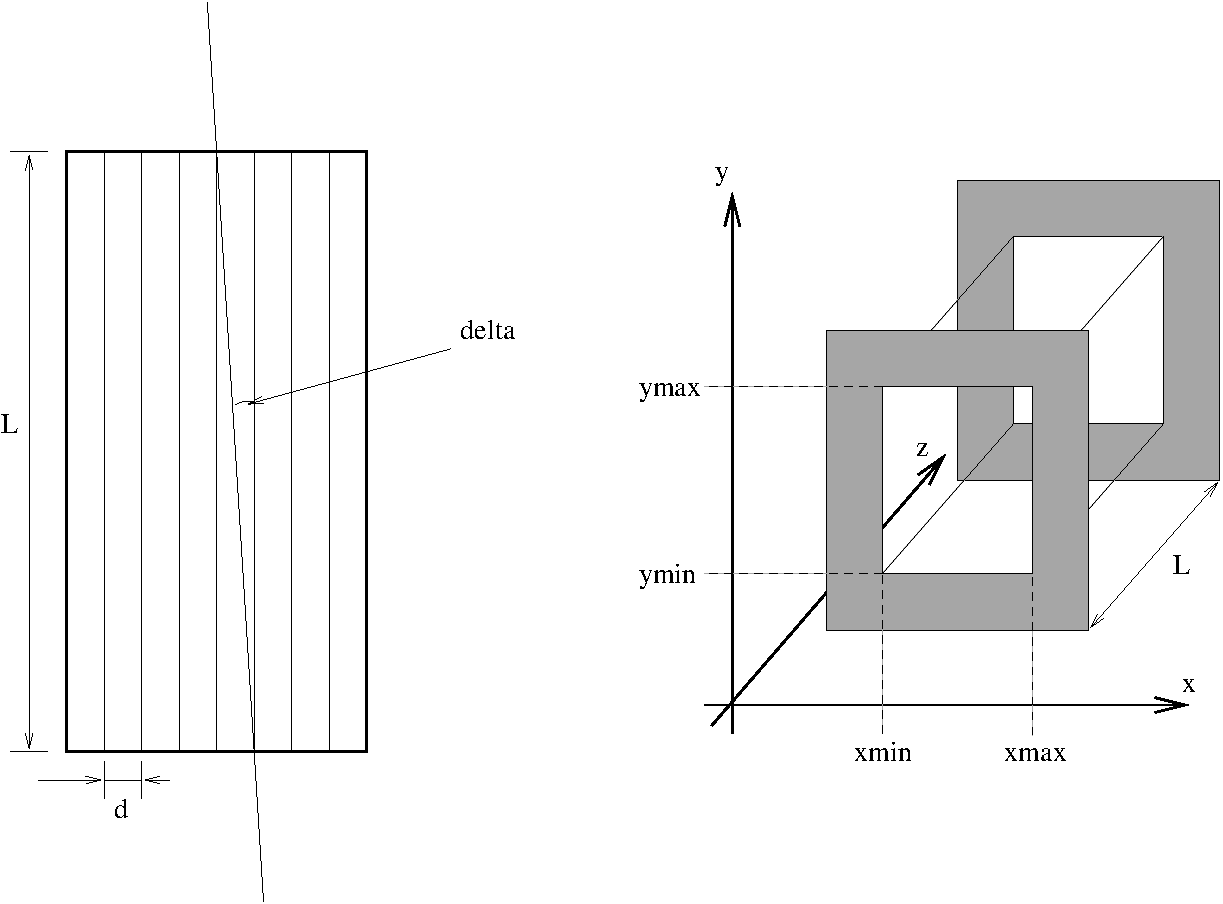
\includegraphics[width=0.7\textwidth]{figures/collimator}
  \end{center}
\caption{The geometry of a simple Soller blade collimators:
The real Soller collimator, seen from the top (left),
and a sketch of the component {\bf Soller} (right).
The symbols are defined in the text.}
\label{f:collimator}
\end{figure}

\subsection{Collimator transmission}
The horizontal divergence, $\eta_h$, is defined as the angle between the
neutron path and the vertical $y-z$ plane along the collimator axis.
We then define the collimation angle as the maximal allowed
horizontal divergence: $\delta = \tan^{-1}(d/L)$,
see Fig.~\ref{f:collimator}. Neutrons with a horizontal
divergence angle $|\eta_h| \geq \delta$ will always
hit at least one collimator blade and will thus be ABSORB'ed.
For smaller divergence angles, $|\eta_h| < \delta$, the fate of the
neutron depends on its exact entry point.
Assuming that a typical collimator has many blades, the
absolute position of each blade perpendicular to the collimator axis
is thus mostly unimportant.
A simple statistical consideration now shows that the transmission
probability is $T = 1-\tan|\eta_h|/\tan\delta$.
Often, the approximation $T \approx 1-|\eta_h|/\delta$ is used, giving
a triangular transmission profile.

\subsection{Algorithm}
The algorithm of {\rm Collimator\_linear} is roughly as follows:
\begin{enumerate}
\item Check by propagation if the neutron ray clear the entry and exit slits,
otherwise ABSORB.
\item Check if $|\eta_h| < \delta$, otherwise ABSORB.
\item Simulate the collimator transmission by a weight transformation:
\begin{equation}
\pi_i = T = 1-\tan|\eta_h|/ \tan\delta ,
\end{equation}
\end{enumerate}


\section{Collimator\_radial: A radial Soller blade collimator}
\index{Optics!Radial collimator}

\component{Collimator\_radial}{(System) E.Farhi, ILL}{$w_1$, $h_1$, $w_2$, $h_2$, $len$, $\theta_{min}$, $\theta_{max}$, $nchan$, $radius$}{$divergence$, $nblades$, $roc$ and others}{Validated}

\begin{figure}
  \begin{center}
    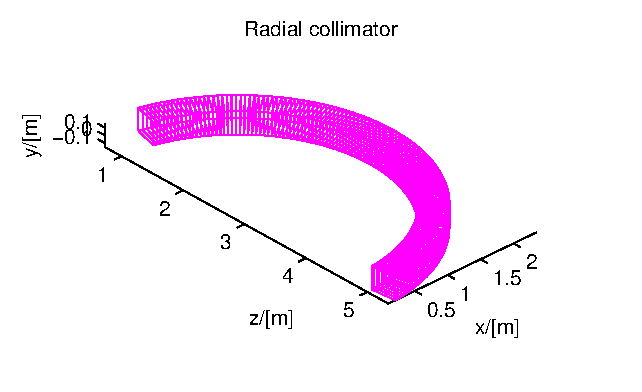
\includegraphics[width=0.8\textwidth]{figures/radial}
  \end{center}
\caption{A radial collimator}
\label{f:coll-radial}
\end{figure}

This radial collimator works either using an analytical approximation
like {\bf Collimator\_linear} (see section \ref{collimator-linear}),
or with an exact model.

The input parameters are the inner radius $radius$, the radial length $len$,
the input and output window dimensions $w_1$, $h_1$, $w_2$, $h_2$,
the number of Soller channels $nchan$
(each of them being a single linear collimator) covering the angular interval
[$\theta_{min}$, $\theta_{max}$] angle with respect to the $z$-axis.

If the $divergence$ parameter is defined,
the approximation level is used as in {\rm Collimator\_linear}
(see section \ref{collimator-linear}).
On the other hand, if you perfer to describe exactly the number of blades
$nblades$ assembled to build a single collimator channel,
then the model is exact, and traces the neutron trajectory inside each Soller.
The computing efficiency is then lowered by a factor 2.

The component can be made oscillating with an amplitude of $roc$ times
$\pm w_1$, which supresses the channels shadow.

As an alternative, you may use the {\bf Exact\_radial\_coll} contributed component.
For a rectangular shaped collimator, instead of cylindrical/radial, you may use the Guide\_channeled and the Guide\_gravity components.


\newpage
\chapter{Reflecting optical components: mirrors, and guides}
\index{Optics|textbf}

This section describes advanced neutron optical
components such as supermirrors and guides as well as various rotating choppers.
A description of the reflectivity of a supermirror is found
in section~\ref{s:mirror}.


\index{Optics|textbf}

This section describes advanced neutron optical
components such as supermirrors and guides.
A description of the reflectivity of a supermirror is found
in section~\ref{s:mirror}.

\section{Mirror: The single mirror}
\label{s:mirror}
\index{Optics!Mirror plane}
\component{Mirror}{System}{$l$, $h$, $m$}{$R_0, Q_c, W, \alpha, reflect$}{validated, no gravitation support}

The component {\bf Mirror}
models a single rectangular neutron mirror plate. It can be used
as a sample component or to \textit{e.g.}~assemble a complete neutron guide by putting multiple
mirror components at appropriate locations and orientations in the
instrument definition, much like a real guide is build from individual
mirrors.

In the local coordinate system, the mirror lies in the first quadrant of the
$x$-$y$ plane, with one corner at $(0,0,0)$.

The input parameters of this component are
the rectangular mirror dimensions $(l, h)$
and the values of $R_0, m, Q_c, W$, and $\alpha$ for the mirror reflectivity.
As a special case, if $m=0$ then the reflectivity is zero for all $Q$,
\textit{i.e.}\ the surface is completely absorbing.

This component may produce wrong results with gravitation.

\subsection{Mirror reflectivity}
\label{ss:mirrorreflect}
To compute the reflectivity of the supermirrors, we use an empirical
formula derived from experimental data \cite{pb_241_50},
see Fig.~\ref{f:reflectivity}. The reflectivity is given by
\begin{equation} \label{e:Rmirror}
  R = \left\{
    \begin{array}{ll}
      R_0 & \textrm{if $Q \leq Q_{\rm c}$} \\
      \frac{1}{2}R_0(1 - \tanh[(Q - m Q_{\rm c})/W])(1-\alpha(Q-Q_{\rm c}))
         & \textrm{if $Q > Q_{\rm c}$}
    \end{array}
  \right.
\end{equation}

Here $Q$ is the length of the scattering vector (in \AA$^{-1}$)
defined by
\begin{equation} \label{e:reflectivity}
Q = |{\bf k}_{\bf i} - {\bf k}_{\bf f}|
  = \frac{m_{\rm n}}{\hbar} |{\bf v}_{\bf i} - {\bf v}_{\bf f}|,
\end{equation}
$m_{\rm n}$ being the neutron mass.
The number $m$ in (\ref{e:Rmirror}) is a parameter determined by
the mirror materials,
the bilayer sequence, and the number of bilayers.
As can be seen, $R=R_0$ for $Q < Q_{\rm c}$, where $Q_{\rm c}$ is the
critical scattering wave vector for a single layer of the mirror
material. At higher values of $Q$, the reflectivity starts falling
linearly with a slope $\alpha$ until a "soft cut-off" at $Q = m Q_{\rm c}$.
The width of this cut-off is denoted $W$. See the example reflection curve in
figure~\ref{f:reflectivity}.

It is {\bf important} to notice that when $m < 1$, the reflectivity remains constant at $R=R_0$ up to $q=Qc$, and \emph{not} $m.Q_c$. This means that $m < 1$ parameters behave like $m=1$ materials.

Alternatively, the Mirror, Guide and Guide\_gravity components may use a reflectivity table $reflect$, which 1st column is q [$\AA^{-1}$] and 2nd column as the reflectivity $R$ in [0-1]. For this purpose, we provide $m=2$ and $m=3$ reflectivity files from SwissNeutronics (\verb+supermirror_m2.rfl+ and \verb+supermirror_m3.rfl+ in \verb+MCSTAS/lib/data/+).

\subsection{Algorithm}
The function of the component can be described as
\begin{enumerate}
\item Propagate the neutron ray to the plane of the mirror.
\item If the neutron trajectory intersects the mirror plate, it is
reflected, otherwise it is left untouched.
\item Reflection of the incident velocity
${\bf v}_{\rm i} = (v_x,v_y,v_z)$
gives the final velocity ${\bf v}_{\rm f} = (v_x,v_y,-v_z)$.
\item Calculate $Q=2 m_{\rm n} v_z / \hbar$.
\item The neutron weight is adjusted with the amount $\pi_i = R(Q)$.
\item  To avoid spending large amounts of computation time on very low-weight
neutrons, neutrons for which the reflectivity is lower than about
$10^{-10}$ are ABSORB'ed.
\end{enumerate}

\begin{figure}
  \begin{center}
    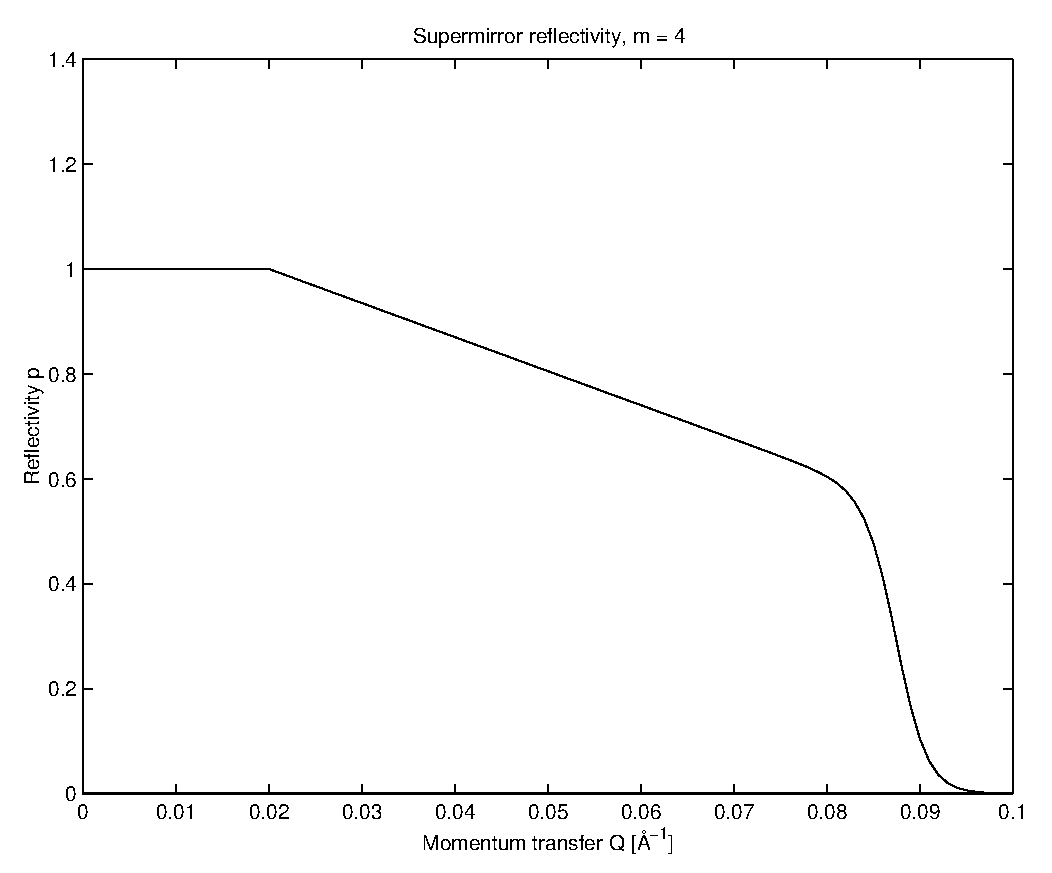
\includegraphics[width=0.6\textwidth]{figures/supermirror.eps}
  \end{center}
\caption{A typical reflectivity curve for a supermirror,
Eq.~(\protect\ref{e:reflectivity}). The used values are
$ m=4$, $R_0=1$, $Q_{\rm c} = 0.02$~\AA$^{-1}$, $\alpha = 6.49$~\AA,
$ W=1/300$~\AA$^{-1}$.
}
\label{f:reflectivity}
\end{figure}

\newpage

\section{Guide: The guide section}
\index{Optics!Straight guide}

\component{Guide}{System}{$w_1, h_1$, $w_2, h_2$, $l$, $m$, $reflect$}{$R_0, Q_c, W, \alpha$}{validated, no gravitation support}

The component {\bf Guide}
models a guide tube consisting of four flat mirrors. The
guide is centered on the $z$ axis with rectangular entrance and exit
openings parallel to the $x$-$y$ plane. The entrance has the dimensions
$(w_1,h_1)$ and placed at $z=0$. The exit is of dimensions $(w_2,h_2)$
and is placed at $z=l$ where $l$ is the guide length. See
figure~\ref{f:guide}.
The reflecting properties are given by the values of
$R_0, m, Q_c, W$, and $\alpha$, as for {\bf Mirror}, or alternatively from the reflectivity file $reflect$.

{\bf Guide} may produce wrong results with gravitation support.
Use {\bf Guide\_gravity} (section \ref{s:guide_gravity}) in this case,
or the {\bf Guide\_channeled}
in section~\ref{s:channeled_guide}.

\begin{figure}
  \begin{center}
    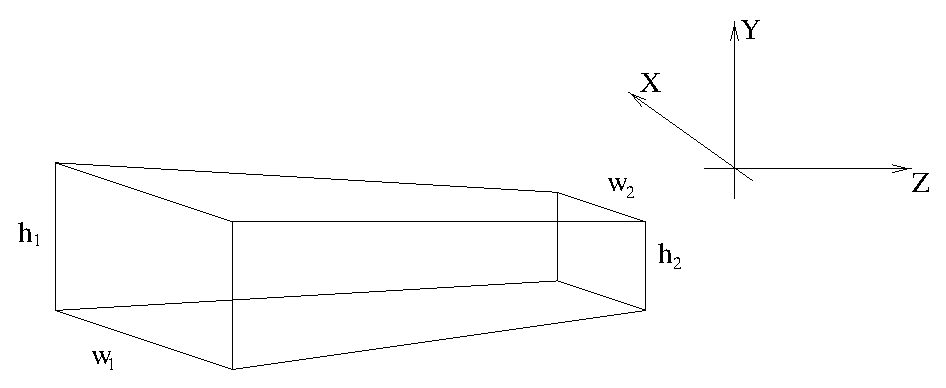
\includegraphics[width=0.7\textwidth]{figures/guide1.eps}
  \end{center}
\caption{The geometry used for the guide component.}
\label{f:guide}
\end{figure}

\subsection{Guide geometry and reflection}
For computations on the guide geometry, we define the planes of the four
guide sides by giving their normal vectors (pointing into the guide)
and a point lying in the plane:
$$
\begin{array}{rclcrcl}
{\bf n}^v_1 &=& (l, 0, {(w_2 - w_1) / 2})
     & & {\bf O}^v_1 &=& (- w_1 / 2, 0, 0) \\
{\bf n}^v_2 &=& (-l, 0, {(w_2 - w_1) / 2})
     & & {\bf O}^v_2 &=& (w_1 / 2, 0, 0) \\
{\bf n}^h_1 &=& (0, l, {(h_2 - h_1) / 2})
     & & {\bf O}^h_1 &=& (0, - h_1 / 2, 0) \\
{\bf n}^h_2 &=& (0, -l, {(h_2 - h_1) / 2})
     & & {\bf O}^h_2 &=& (0, h_1 / 2, 0) \\
\end{array}
$$
In the following, we refer to an arbitrary guide side by its origin
{\bf O} and normal {\bf n}.

With these definitions, the time of intersection of the neutron with a
guide side can be computed by considering the projection onto the
normal:
\begin{equation}
t^\alpha_\beta = \frac{({\bf O}^\alpha_\beta - {\bf r}_0) \cdot {\bf n}^\alpha_\beta}
  {{\bf v} \cdot {\bf n}^\alpha_\beta}  ,
\end{equation}
where $\alpha$ and $\beta$ are indices for the different guide walls,
assuming the values (h,v) and (1,2), respectively.
For a neutron that leaves the guide directly through the guide exit we have
\begin{equation}
t_{\rm exit} = \frac{l - z_0}{v_z}
\end{equation}

The reflected velocity ${\bf v}_{\rm f}$ of the neutron with incoming velocity
${\bf v}_{\rm i}$ is computed by the formula
\begin{equation}
 {\bf v}_{\rm f} =
  {\bf v}_{\rm i}
   - 2{{\bf n} \cdot \frac{{\bf v}_{\rm i}}{{|{\bf n}|^2}} {\bf n}}
\end{equation}
This expression is arrived at by again considering the projection onto
the mirror normal (see figure~\ref{f:guidereflect}). The reflectivity of the
mirror is taken into account as explained in section~\ref{s:mirror}.

\begin{figure}
  \begin{center}
    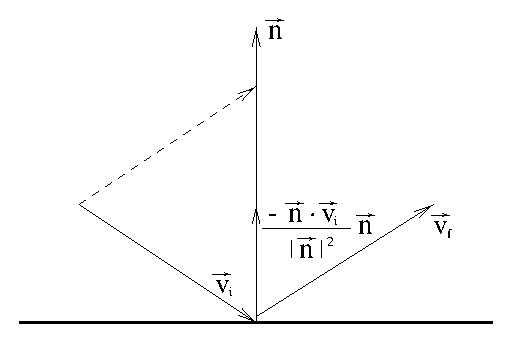
\includegraphics[width=0.5\textwidth]{figures/guide2.eps}
  \end{center}
\caption{Neutron reflecting from mirror. ${\bf v}_{\rm i}$ and
${\bf v}_{\rm f}$ are the initial and final velocities, respectively,
and {\bf n} is a vector normal to the mirror surface.}
\label{f:guidereflect}
\end{figure}

\subsection{Algorithm}
\begin{enumerate}
\item The neutron is initially propagated to the $z = 0$ plane of the
guide entrance.
\item If it misses the entrance, it is ABSORB'ed.
\item Otherwise, repeatedly compute the time of intersection with the
four mirror sides and the guide exit.
\item The smallest positive $t$ thus
found gives the time of the next intersection with the guide (or in the
case of the guide exit, the time when the neutron leaves the guide).
\item Propagated the neutron ray to this point.
\item Compute the reflection from the side.
\item Update the neutron weight factor by the amount $\pi_i = R(Q)$.
\item Repeat this process until the neutron leaves the guide.
\end{enumerate}

There are a few optimizations possible here to avoid redundant
computations. Since the neutron is always inside the guide during the
computations, we always have
$({\bf O} - {\bf r}_0) \cdot {\bf n} \leq 0$.
Thus $t \leq 0$ if ${\bf v} \cdot {\bf n} \geq 0$, so in this case
there is no need to actually compute $t$. Some redundant computations
are also avoided by utilizing symmetry and the fact that many
components of {\bf n} and {\bf O} are zero.

\newpage

\section{Guide\_channeled: A guide section component with multiple channels}
\label{s:channeled_guide}
\index{Optics!Guide with channels (straight, non focusing)}

\component{Guide\_channeled}{System}{$w_1, h_1$, $w_2, h_2$, $l$, $k$, $m_x, m_y$}{$d, R_0, Q_{cx}, Q_{cy}, W, \alpha_x, \alpha_y$}{validated, no gravitation support}

The component {\bf Guide\_channeled} is a more complex variation of {\bf Guide}
described in the previous section. It allows the specification
of different supermirror parameters for the horizontal and vertical
mirrors, and also implements guides with multiple channels as used in
neutron bender devices. By setting the $m$ value of the supermirror
coatings to zero, nonreflecting walls are simulated;
this may be used for a very detailed simulation of a Soller collimator,
see section~\ref{collimator-linear}.

The input parameters are $w_1$, $h_1$, $w_2$, $h_2$, and $l$
to set the guide dimensions as for {\bf Guide}
(entry window, exit window, and length);
$k$ to set the number of channels; $d$ to set the thickness of the
channel walls; and $R_0$, $W$, $Q_{cx}$, $Q_{cy}$, $\alpha_x$, $\alpha_y$,
$m_x$, and $m_y$ to set the supermirror parameters as described under {\bf Guide}
(the names with \textit{x} denote the vertical mirrors,
and those with \textit{y} denote the horizontal ones).

\subsection{Algorithm}
The implementation is based on that of {\bf Guide}.
\begin{enumerate}
\item Calculate the channel which the neutron will enter.
\item Shift the $x$ coordinate so that the channel can be simulated
as a single instance of the {\bf Guide} component.
\item (do the same as in {\bf Guide}.)
\item Restore the coordinates when the
neutron exits the guide or is absorbed.
\end{enumerate}

\subsection{Known problems}\index{Bugs}
\begin{itemize}
\item This component may produce wrong results with gravitation support.
Use Guide\_gravity (section \ref{s:guide_gravity}) in this case.
\item The focusing channeled geometry (for $k > 1$ and different
values of $w_1$ and $w_2$) is buggy
(wall slopes are not computed correctly, and the component 'leaks' neutrons).
\end{itemize}
\newpage

\section{Guide\_gravity: A guide with multiple channels and gravitation handling}
\label{s:guide_gravity}
\index{Optics!Guide with channels and gravitation handling (straight)}
\index{Optics!Fermi Chopper}

\component{Guide\_gravity}{System}{$w_1, h_1$, $w_2, h_2$, $l$, $k$, $m$}{$d, R_0, Q_c, W, \alpha$, wavy, chamfers, $k_h$, $n$, $G$}{validated, {\bf with} gravitation support, rotating mode}

This component is a variation of {\bf Guide\_channeled}
(section \ref{s:channeled_guide}) with the ability to handle
gravitation effects and functional channeled focusing geometry.
Channels can be specified in two dimensions,
producing a 2D array ($k, k_h$) of smaller rectangular guide channels.

The coating is specified as for the Guide and Mirror components by mean of the parameters $R_0, m, Q_c, W$, and $\alpha$, or alternatively from the reflectivity file $reflect$.

Waviness effects, supposed to be randomly distributed
(\emph{i.e.} non-periodic waviness)
can be specified globally, or for each part of the guide section.
Additionally, chamfers
may be defined the same way.
Chamfers originate from the substrate manufacturing, so that operators do not harm themselves with cutting edges. Usual dimensions are about tens of millimeters. They are treated as absorbing edges around guide plates, both on the input and output surfaces, but also aside each mirror.

The straight section of length $l$ may be divided into $n$ bits of same length
within which chamfers are taken into account.

The component has also the capability to rotate at a given frequenccy in order to approximate a Fermi Chopper, including phase shift. The approximation resides in the fact that the component is considered fixed during neutron propagation inside slits. Beware that this component is then located at its entry window (not centered as the other Fermi choppers).\index{Bugs}

To activate gravitation support, either select the \MCS\ gravitation support (\verb+mcrun --gravitation ...+ or from the Run dialog of \verb+mcgui+),
or set the gravitation field strength $G$ (e.g. -9.81 on Earth).

This component is about 50 \% slower than the \verb+Guide+ component, but has much more capabilities.

A contributed version Guide\_honeycomb of this component exists with a honeycomb geometry.

\section{Bender: a bender model (non polarizing)}
\index{Optics!Bender (non polarizing)}

\component{Bender}{Philipp Bernhardt}{$r, W_{in},l,w,h $}{$k,d,R_{0[a,i,s]},\alpha_{[a,i,s]},m_{[a,i,s]},Q_{c[a,i,s]},W_{[a,i,s]}$}{partly validated, no gravitation support}

The Bender component is simulating an ideal curved neutron guide (bender). It is bent to the negative X-axis and behaves like a parallel guide in the Y axis. Opposite curvature may be achieved by a $(0,0,180)$ rotation (along Z-axis).

Bender radius $r$, entrance width $w$ and height $h$ are required parameters. To define the length, you may either enter the deviation angle $W_{in}$ or the length $l$. Three different reflectivity profiles $R_0,Q_c,W,m,\alpha$ can be given (see section~\ref{s:mirror}): for outer
walls (index $a$), for inner walls (index $i$) and for the top and bottom walls (index $s$).

To get a better transmission coefficient, it is possible to split the bender into $k$ channels which are separated by partitions with the thickness of $d$. The partitioning walls have the same coating as the exterior walls.

Because the angle of reflection doesn't change, the routine
calculates the reflection coefficent for the concave and, if necessary, for the convex wall only onces, together with the number of reflections.
Nevertheless the exact position, the time, and the divergence is calculated at the end of the bender, so there aren't any approximations.

The component is shown \emph{straight} on geometrical views (mcdisplay/Trace), and the next component may be placed directly at distance $r.W_{in} = l$ \emph{without} rotation.

Results have been compared succesfully with analytical formula in the case of an ideal reflection and cross-checked with the program \verb+haupt+.

An other implementation of the Bender is available as the contributed component Guide\_curved.

\section{Curved guides}
\index{Optics!Curved guides (polygonal model)}

Real curved guides are usually made of many straight elements (about 1 m long) separated with small gaps (e.g. 1 mm). Sections of about 10 m long are separated with bigger gaps for accessibility and pumping purposes.

We give here an example description of such a section. Let us have a curved guide of total length $L$, made of $n$ elements with a curvature radius $R$. Gaps of size $d$ separate elements from each other. The rotation angle of individual straight guide elements is $\alpha_z = (L+d)/R*180/\pi$ in degrees.

In order to build an independent curved guide section, we define \verb+Arm+ components at the begining and end of it.
\begin{verbatim}
COMPONENT CG_In = Arm() AT (...)

COMPONENT CG_1  = Guide_gravity(l=L/n, ...)
AT (0,0,0) RELATIVE PREVIOUS

COMPONENT CG_2  = Guide_gravity(l=L/n, ...)
AT (0,0,L/n+d) RELATIVE PREVIOUS
ROTATED (0, (L/n+d)/R*180/PI, 0) RELATIVE PREVIOUS
...
COMPONENT CG_Out = Arm() AT (0,0,L/n) RELATIVE PREVIOUS
\end{verbatim}
The \verb+Guide+ component should be duplicated $n$ times by copy-paste, but changing the instance name, e.g. CG\_1, CG\_2, ..., CG\_n. This may be automated with the \verb+COPY+ or the \verb+JUMP ITERATE+ mechanisms (see User manual).

An implementation of a continuous curved guide has been contributed as component Guide\_curved.



\chapter{Moving optical components:
Choppers and velocity selectors}
We list in this chapter some moving optical components,
like choppers, that may be used for TOF class instrument simulations,
and velocity selector used for partially monochromatize continuous beams.
\index{Library!Components!optics}
\index{Optics|textbf}

% Emacs settings: -*-mode: latex; TeX-master: "manual.tex"; -*-

\section{DiskChopper: The disc chopper}
\label{s:chopper}
\index{Optics!Disc chopper}

\component{DiskChopper}{Peter Willendrup, Ris\o\ (System)}{$\theta_0$,
  $R$, $h$, $\omega$, $n$, $t_0$, $\phi_0$}{IsFirst,
  $n_{\rm pulse}$}{Based on Chopper by P Bernhardt, extensions K
  Hewitt Klen\o\ and R Bewey}

To cut a continuous neutron beam into short pulses, or to control
the pulse shape (in time) from a pulsed source, one can use a disc
chopper (see figure~\ref{f:chopper1}). This is a fast rotating disc with the
rotating axis parallel to the neutron beam. The disk consists of neutron
absorbing materials. To form the pulses the disk has openings through which
the neutrons can pass.

Component {\bf DiskChopper} is an infinately thin, absorbing disc of
radius $R$ with $n$ slit openings of height $h$ and angular width
$\theta_0$. The slits are symmetrically disposed on the disc. If
unset, the slit height $h$ will extend to the centre of the disc ($h=R$).

The {\bf DiskChopper} is self-centering, meaning that the centre of
the slit openings will automatically be positioned at the centre of
the beam axis (see figure~\ref{f:chopper1}). To override this behaviour, set the paramter
$compat=1$, positioning the chopper centre at height $-R$ - as
implemented in the original {\bf Chopper} component.

Optionally, each slit can have a central, absorbing insert - a
\emph{beamstop} of angular width $\theta_1$. For more exotic chopper
definitions, use the \texttt{GROUP} keyword, see below for an example.

The direction of rotation can be controlled,
which allows to simulate e.g. counter-rotating choppers.
The phase or time-delay $t_0$ (in seconds) is defined by the time
where the first of the $n$ slits is positioned at the top. As an
alternative, an angular phase can be given using the $\phi_0$ parameter.

By default, neutrons hitting outside the physical extent of the disc
are absorbed. This behaviour can be overruled by setting parameter
$abs\_out=0$.


\begin{figure}[ht]
\centering
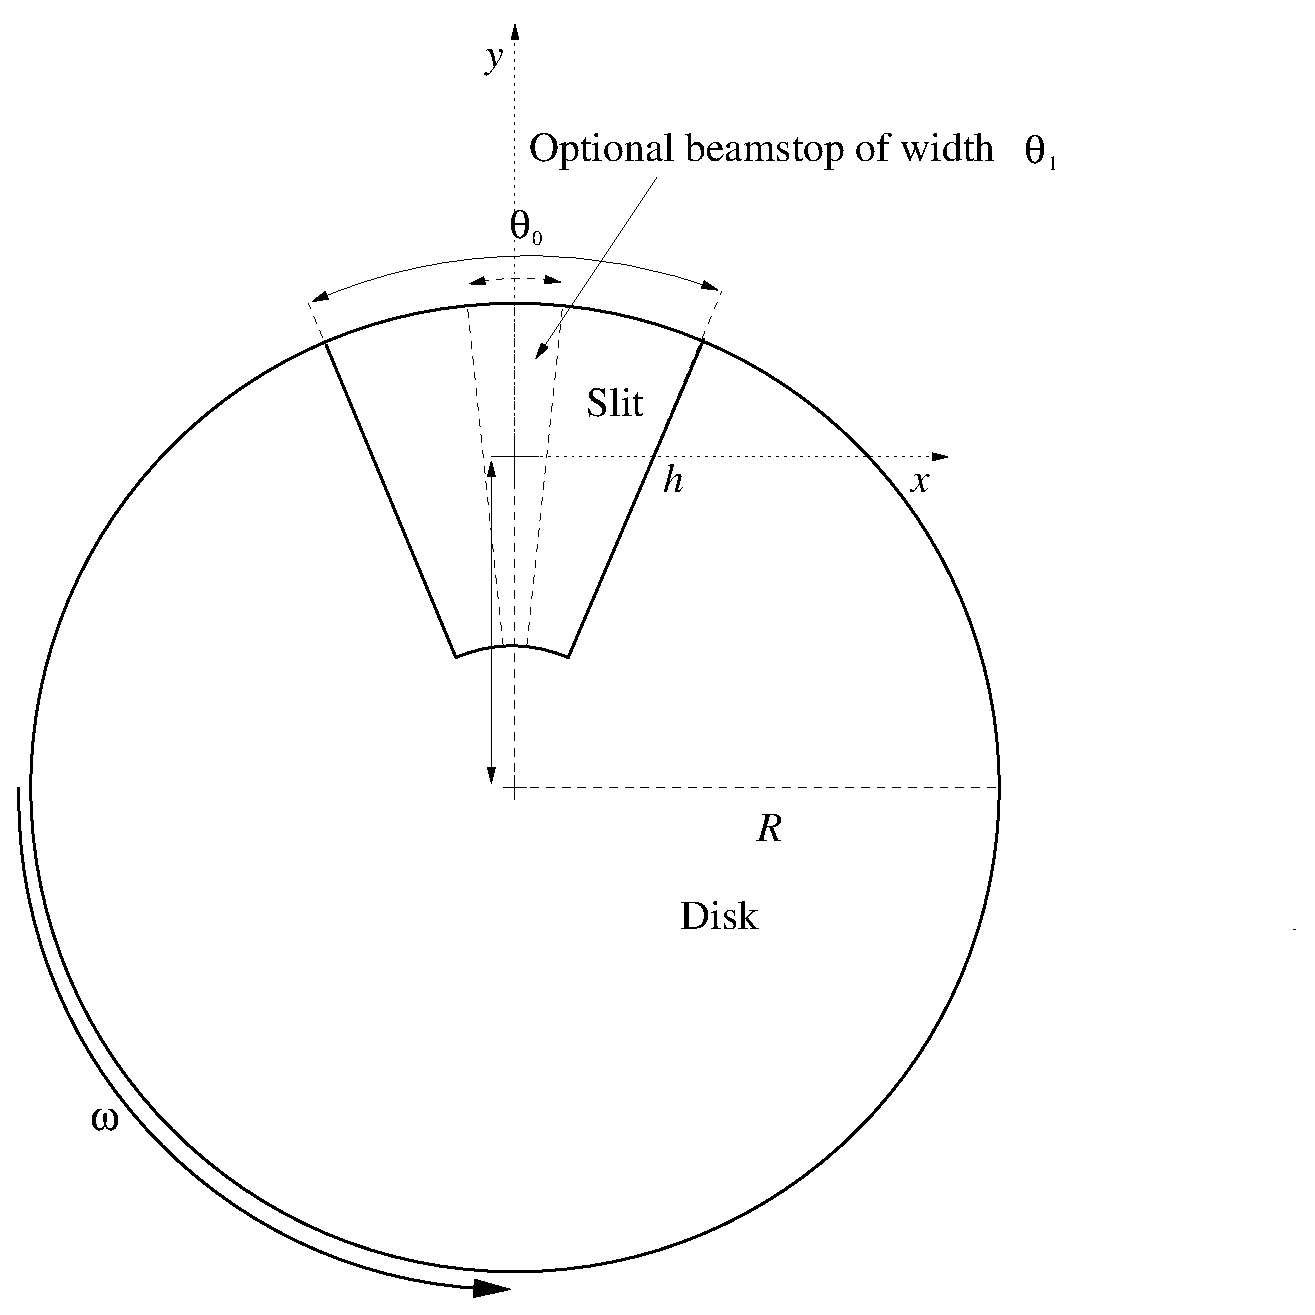
\includegraphics[width=0.8\linewidth]{figures/DiskChopper}
\caption{Sketch of a disc chopper with geometry parameters}
\label{f:chopper1}
\end{figure}


%Using a rectangular shaped beam with nearly the same
%size as the slit, yields an almost triangular shaped
%transmission curve (see figure~\ref{f:chopper2}).
%
%\begin{figure}[ht]
%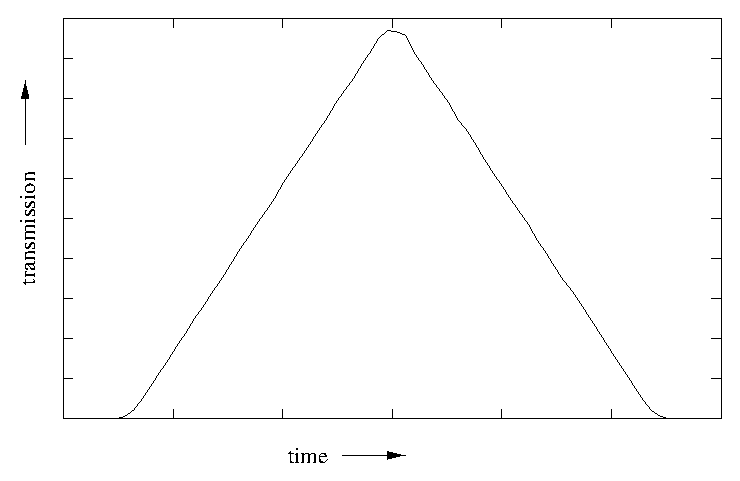
\includegraphics[width=1.0\linewidth]{figures/tracho}
%\caption{example transmission curve for the disc chopper\label{f:chopper2}}
%\end{figure}

When simulating the chopping of a continuous beam,
most of the neutrons could easily be lost.
To improve efficiency, one can set the flag \verb+IsFirst+, which will
allow every neutron ray to pass the {\bf DiskChopper}, but modify the
time, $t$, to a (random) time at which it is possible to pass.
%This can also be used with TOF-instruments, which often
%define the starting time of the neutrons at
%the position of the first chopper.
Of course, there should be only one ``first chopper'' in
any simulation.
To simulate frame overlap from a ``first chopper'', one can specify
the number of frames to study by the parameter $n_{\rm pulse}$.

For more advanced chopper geometries than those mentioned above, it is
possible to set up a \texttt{GROUP} of choppers:

\begin{lstlisting}
COMPONENT Chop1 = DiskChopper(omega=2500, R=0.3, h=0.2, theta_0=20, n=1)
AT (0, 0, 1.1) RELATIVE Source
GROUP Choppers

COMPONENT Chop2 = DiskChopper(omega=2500, R=0.3, h=0.2, theta_0=20, n=1,
                              phi_0=40)
AT (0, 0, 1.1) RELATIVE Source
GROUP Choppers
\end{lstlisting}

The result of such a {\bf DiskChopper} \texttt{GROUP}ing can be seen in
figure \ref{f:chopper2}

\begin{figure}[ht]
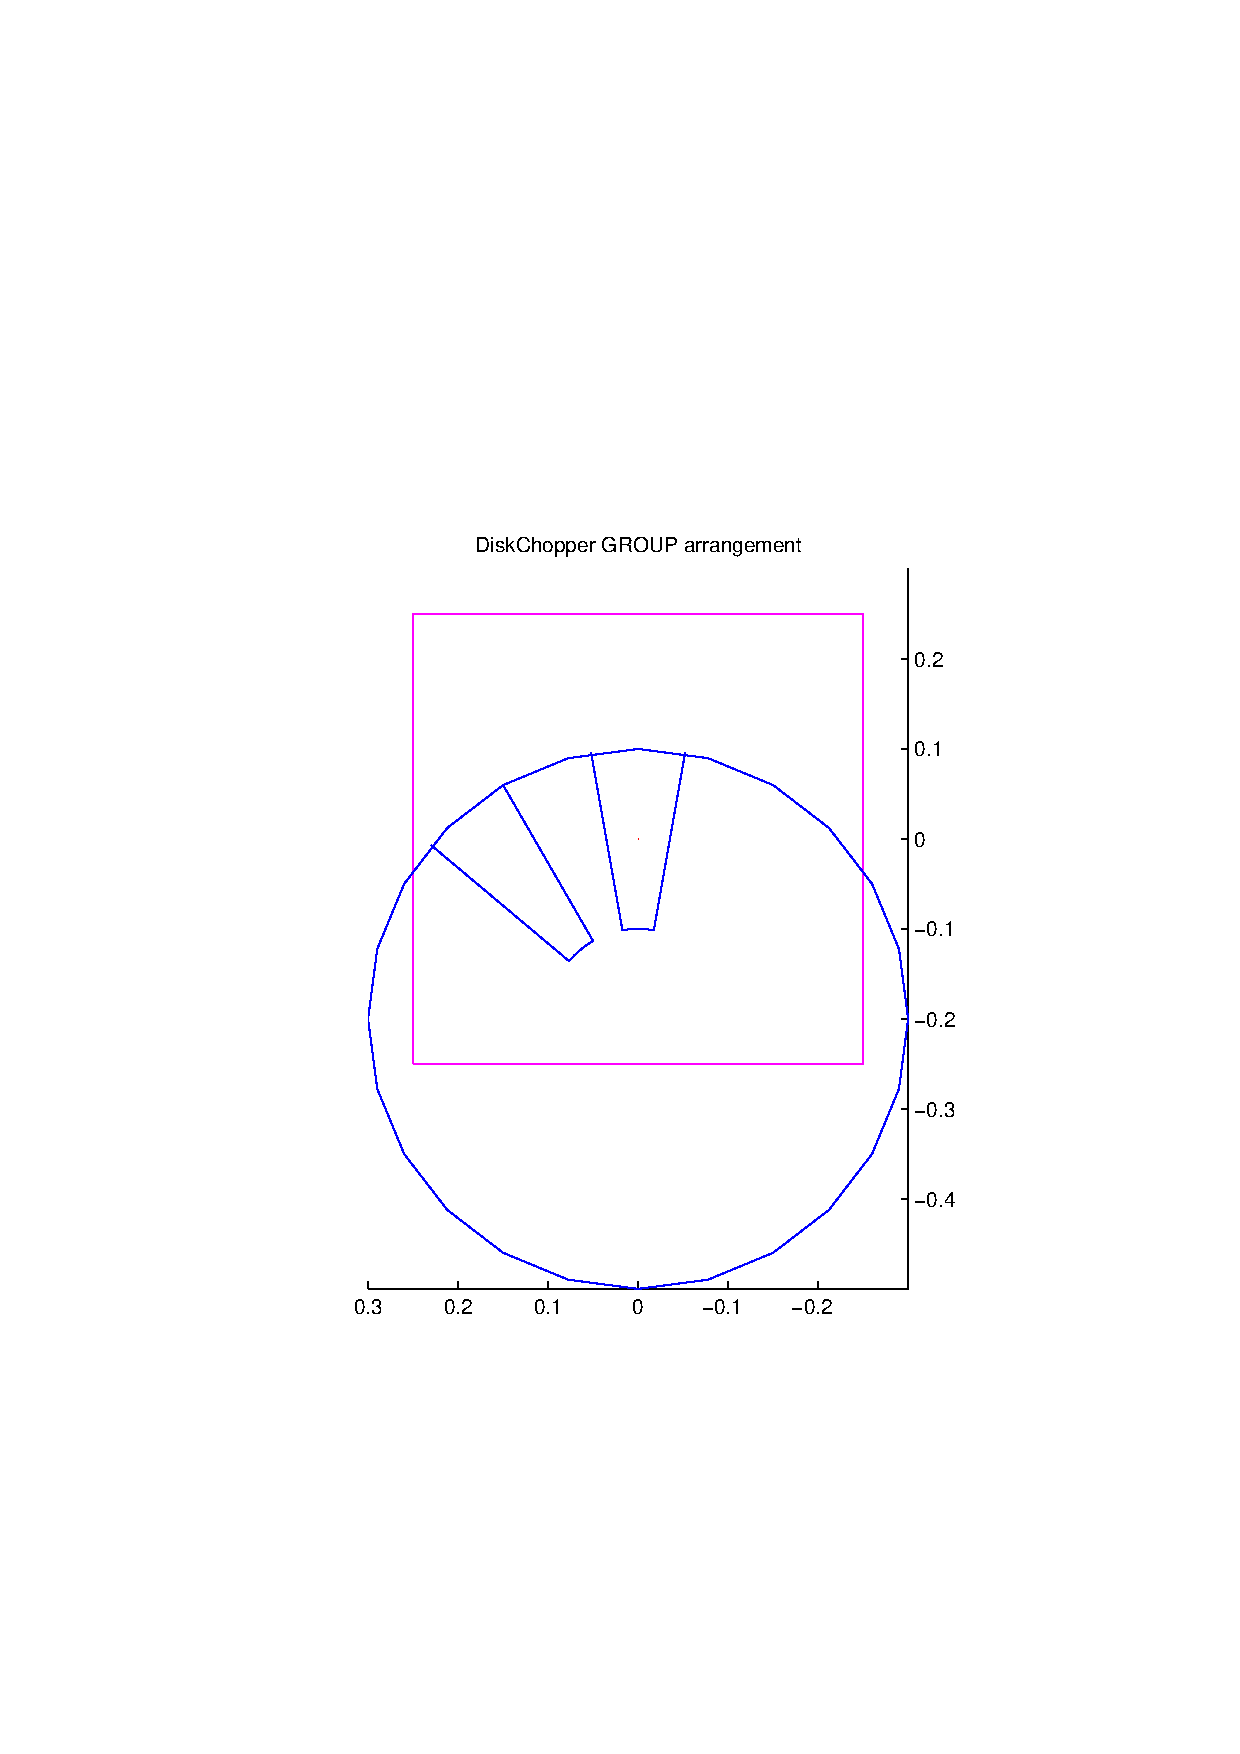
\includegraphics[width=0.4\linewidth]{figures/DiskChopperGroup}
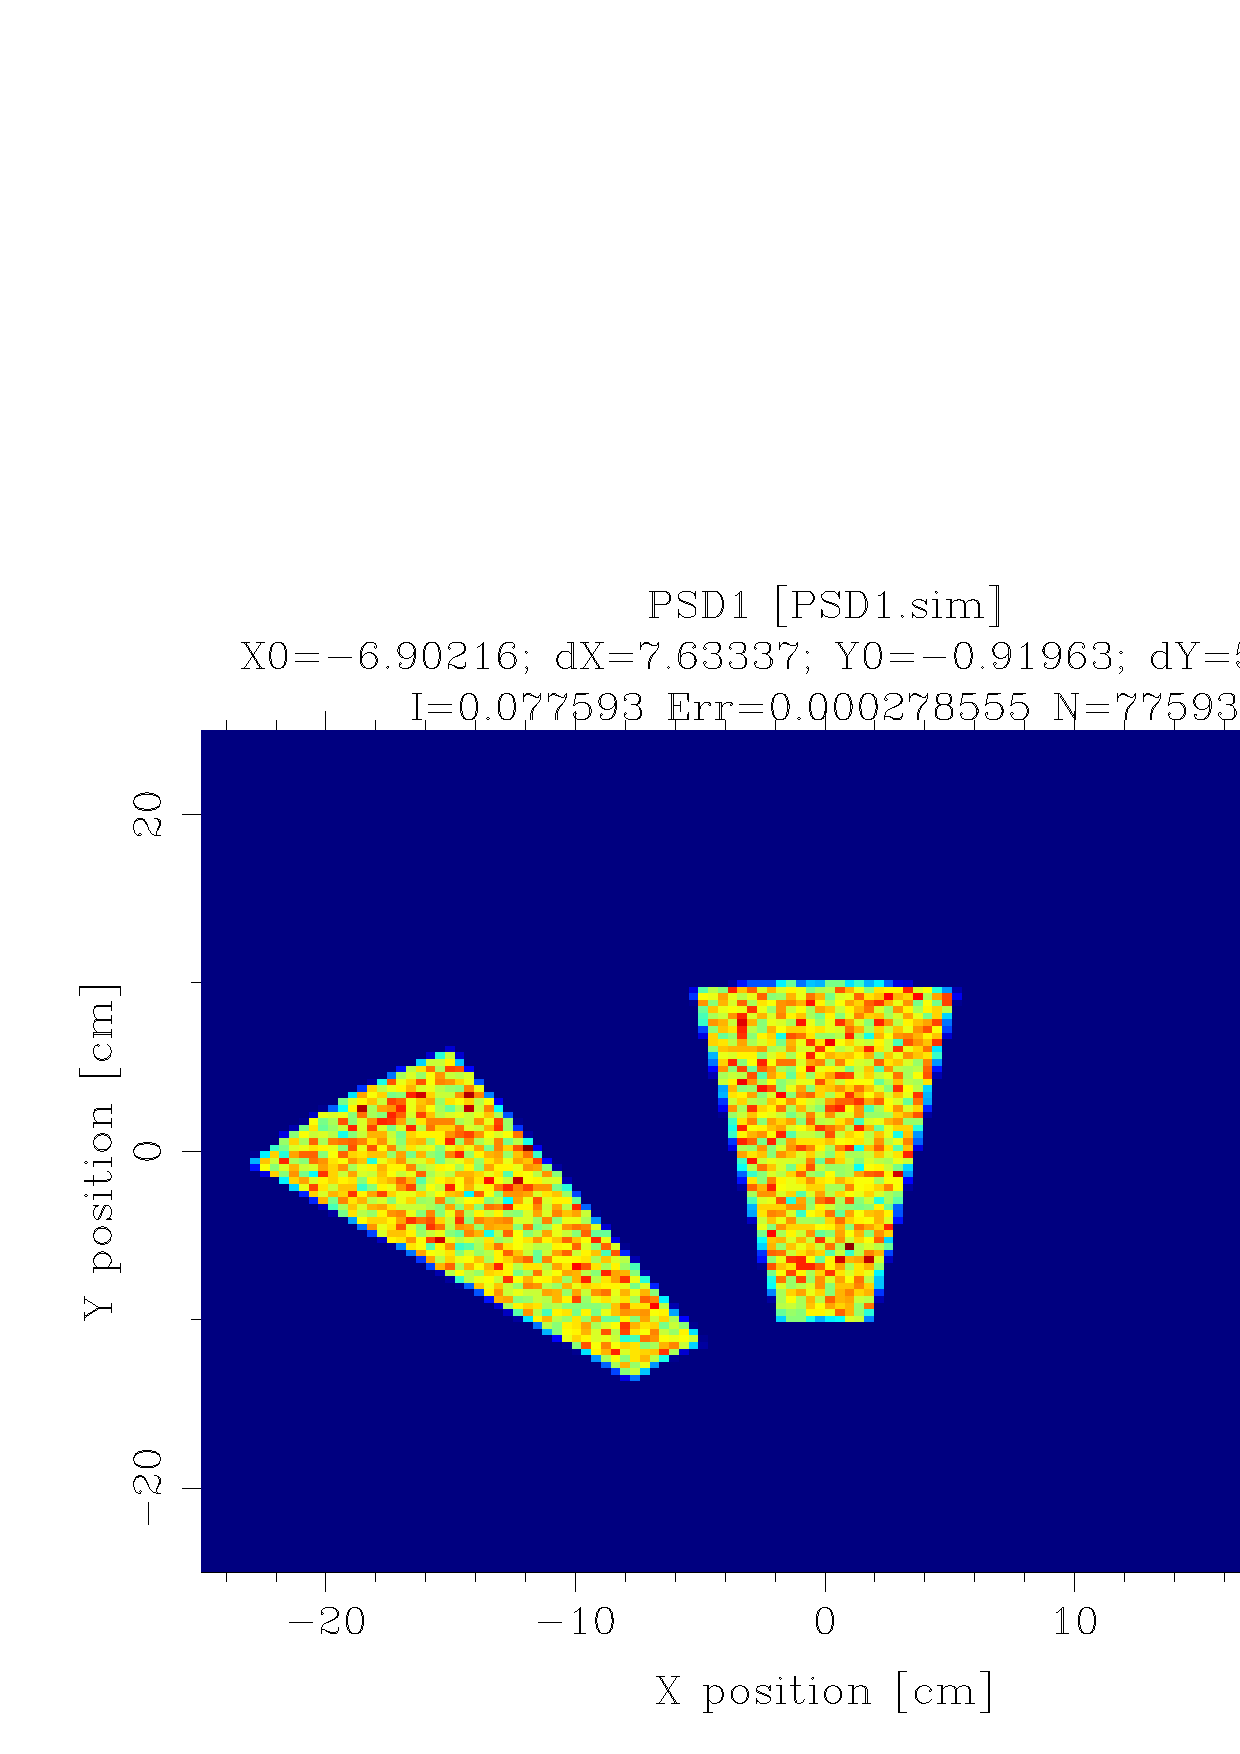
\includegraphics[width=0.4\linewidth]{figures/DiskChopperPSD}
\caption{\texttt{mcdisplay} rendering and monitor output from a DiskChopper \texttt{GROUP}}
\label{f:chopper2}
\end{figure}


\newpage
\section{FermiChopper: The Fermi-chopper}

%\component{FermiChopper}{M. Poehlmann, C. Carbogno, H. Schober,
%E. Farhi}{$R,y_{min} y_{max},
%\nu,w,length$,Nslit,phase}{$m,Q_c,R_0,\alpha,
%W$,curvature,zero\_time}{validated}
\mcdoccomp{optics/FermiChopper.parms}   
\index{Optics!Fermi Chopper|textbf}

\begin{figure}
\begin{center}
\begin{tabular}{cc}
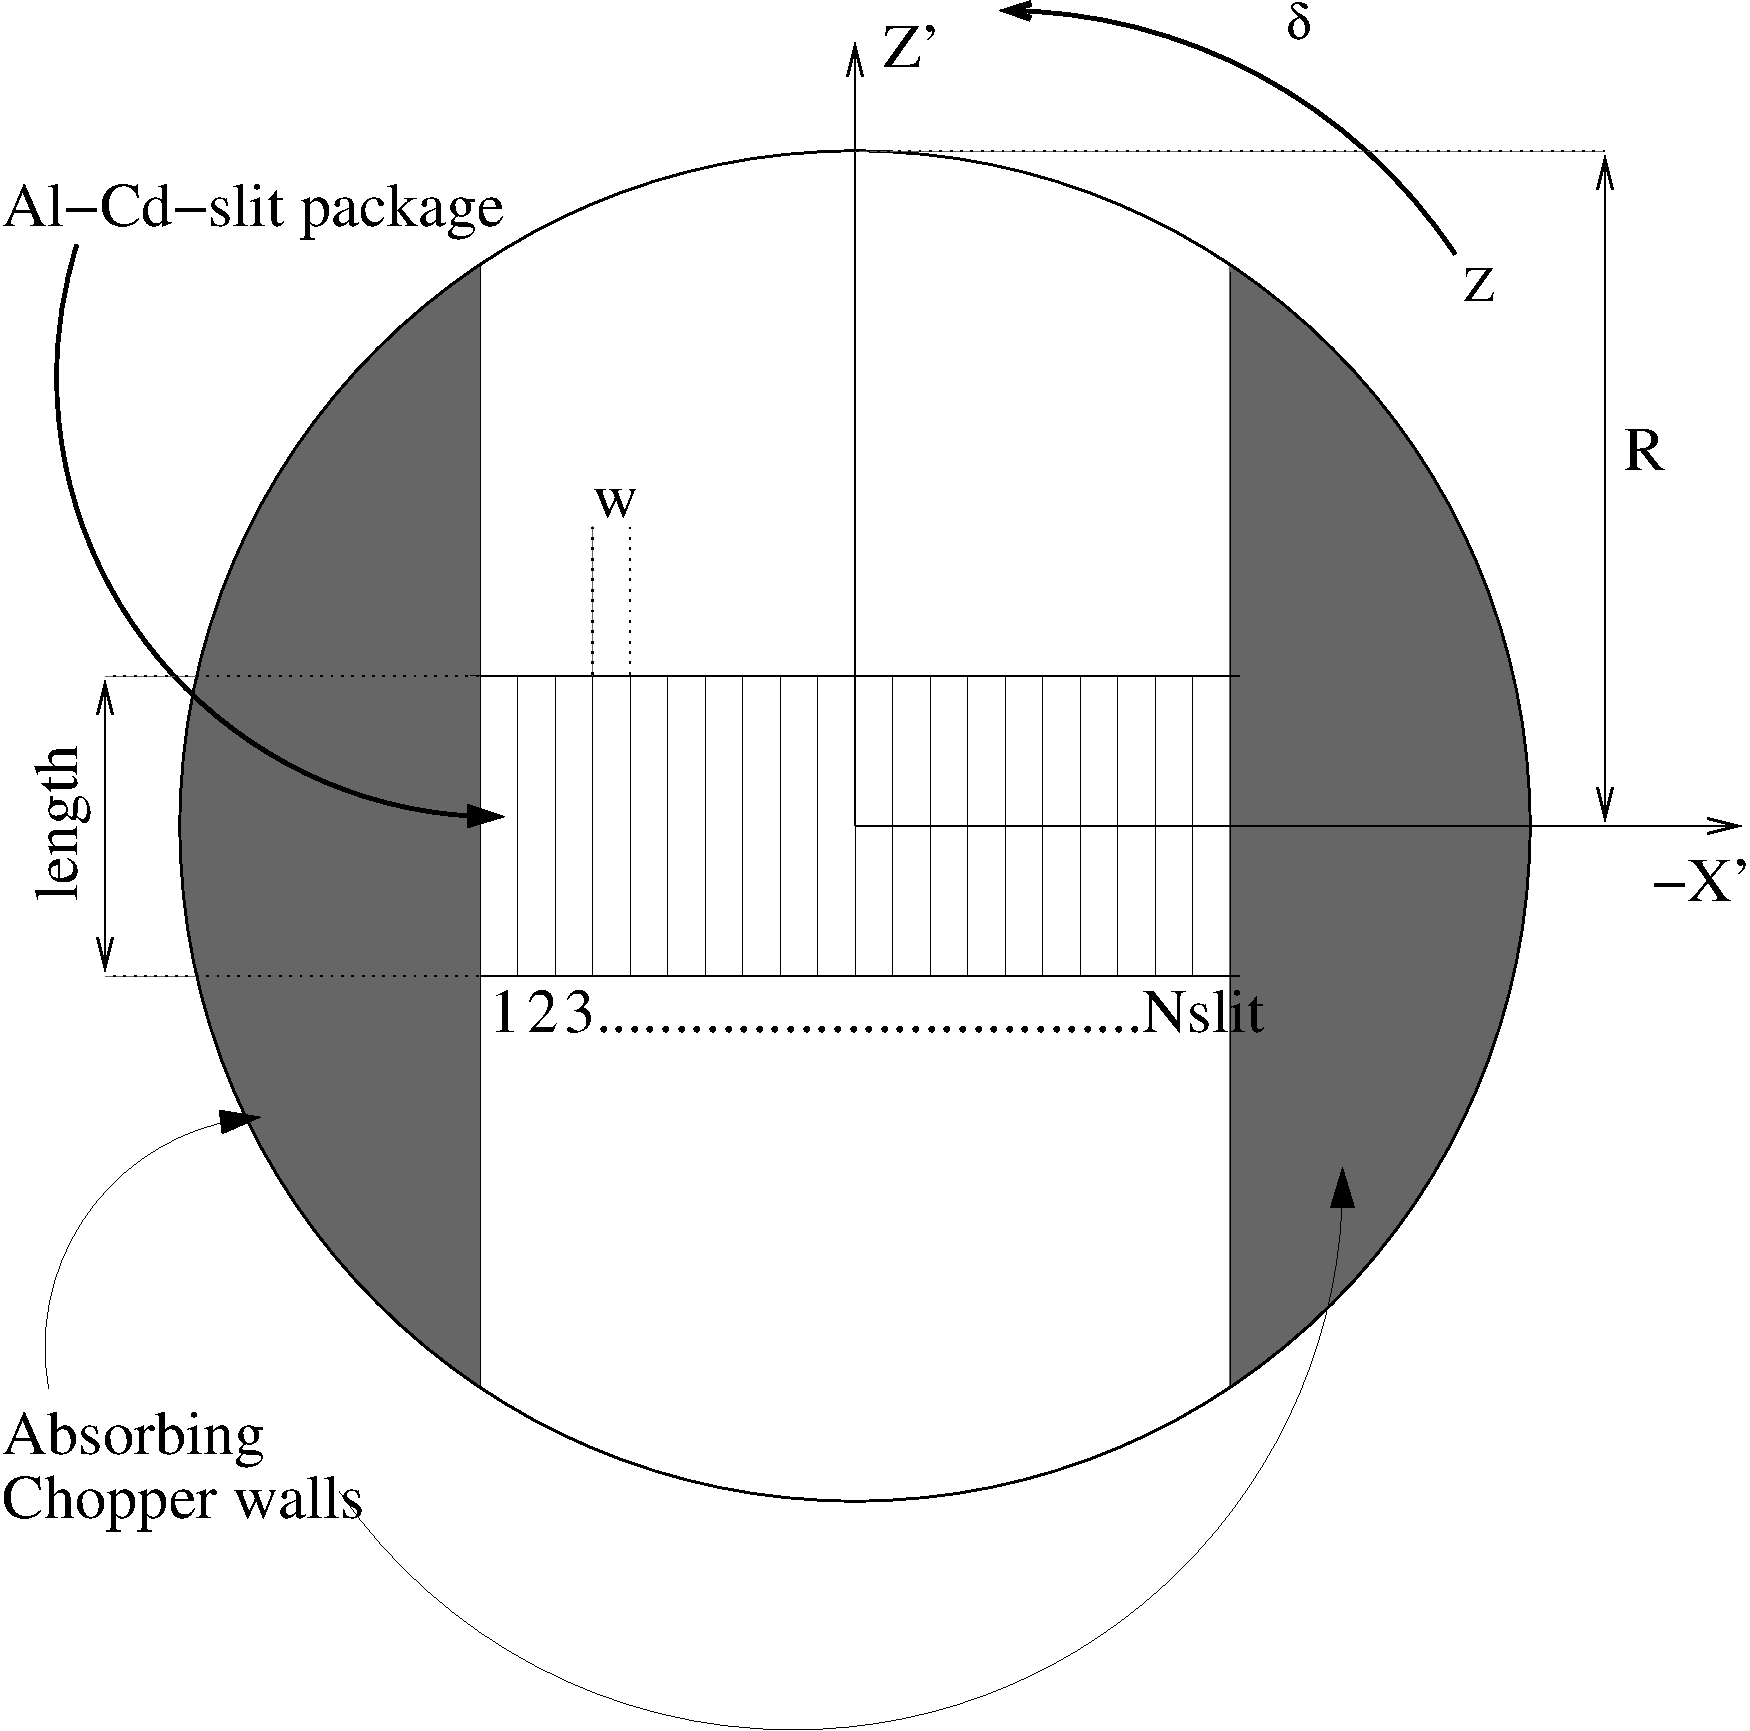
\includegraphics[height=7cm]{./figures/FCChoppergeo}
&
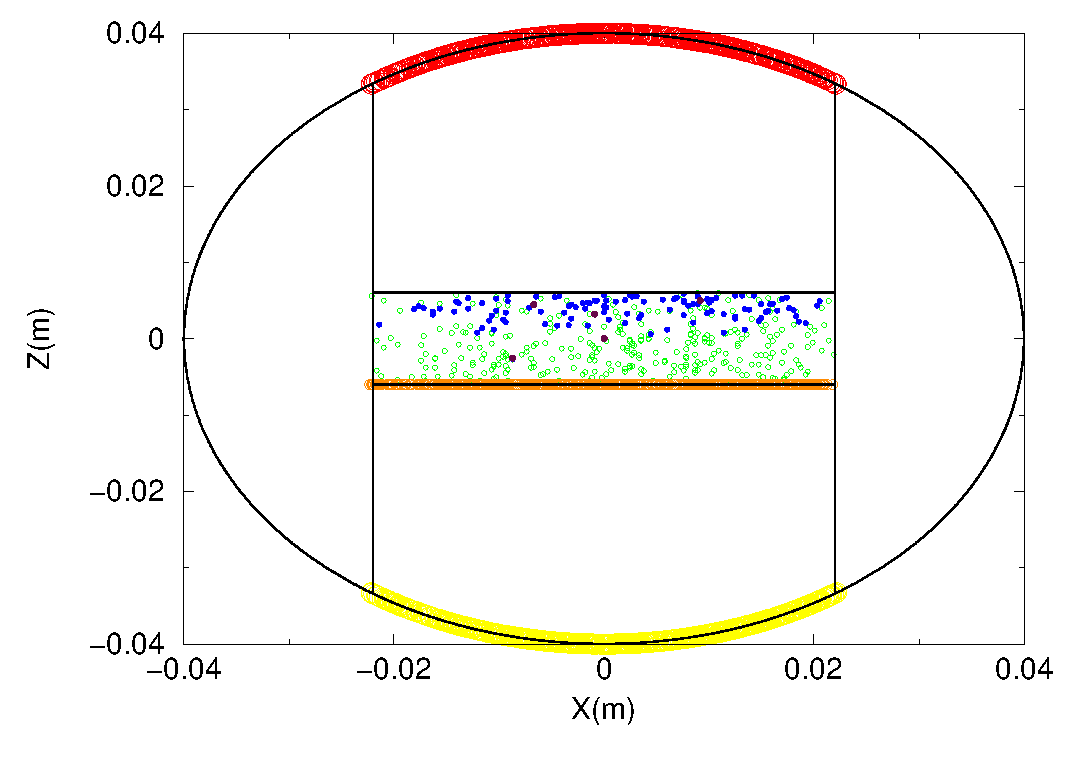
\includegraphics[height=5cm,width=5.3cm]{./figures/FCOverview}
\end{tabular}
\end{center}
\caption{Geometry of the Fermi-chopper (left) and Neutrons in the chopper (right).}
\label{fig:Overview}
\end{figure}

\subsection{The chopper geometry and parameters}
\label{ssec:chopper}

The Fermi chopper is a rotating vertical cylinder containing a set of collimating slits (\emph{slit package}). Main geometry parameters are the radius $R$, minimum and maximum height $y_{min}$ and $y_{max}$ (see Fig. \ref{fig:Overview}).
In this implementation, the slits are by default straight, but may be coated with super-mirror, and curved. Main parameters for the slits are the number of slits $Nslit$, the length $length$ and width $w$ of each slit, the width of the separating Cd-blades is neglected. The slit walls reflectivity is modelled just like in guide components by the $m$-value ($m > 1$ for super mirrors), the critical scattering vector $Q_c$, the slope of reflectivity $\alpha$, the low-angle reflectivity $R_0$ and the width of supermirror cut-off $W$. For $m=0$ the blades are completly absorbing. The AT position of the component is its center.

The angular speed of the chopper is $\omega = 2\pi \nu$, where $\nu$ is the rotation frequency. The angle $phase$ for which the chopper is in the 'open' state for most of the neutrons coming in (z' axis of the rotating frame parallel to the z axis of the static frame) is also an input parameter. The time window may optionally be shifted to zero when setting the \verb+zero_time=1+ option. A phase guess value may be set automatically using the \verb+zero_time=2+ option.

The curvature of the slit channels is specified with the \textit{curvature} parameter. Positive sign indicates that the deviation 'bump' due to curvature is in the $x'$ positive side, and the center of curvature is in the $x'$ negative side. The optimal radius of curvature $R$ is related to frequency $\nu$ and neutron velocity $v$ with: $v=4 \pi R \nu$.

The component was validated extensively by K.\ Lieutenant. As an alternative, one may use the \textbf{Vitess\_ChopperFermi} component (eventhough slower and without super-mirror support) or the \textbf{FermiChopper\_ILL} contributed component. The Guide\_gravity component has also a rotating mode, using an approximation of a Fermi Chopper.

\begin{table}
  \begin{center}
  {\let\my=\\
    \begin{tabular}{|lr|p{0.6\textwidth}|}
    \hline
Parameter & unit & meaning \\
    \hline
radius & [m] & chopper cylinder radius \\
ymin   & [m] &   lower y bound of cylinder \\
ymax   & [m] &   upper y bound of cylinder \\
Nslit  & [1] &   number of chopper slits \\
length & [m] &   channel length of the Fermi chopper \\
w      & [m] &   width of one chopper slit. May also be specified as \emph{width}=w*Nslit for total width of slit package. \\
nu & [Hz] &  chopper frequency \\
phase     & [deg] &   chopper phase at t=0 \\
zero\_time & [1] & shit time window around 0 if true \\
curvature & [m$^{-1}$] & Curvature of slits (1/radius of curvature) \\
    \hline
m     & [1] & \\
alpha & [\AA] & \\
Qc    & [\AA$^{-1}$] & slit coating parameters. See section \ref{ss:mirrorreflect} \\
W     & [\AA$^{-1}$] & \\
R0    & [1] & \\
    \hline
    \end{tabular}
    \caption{FermiChopper component parameters}
    \label{t:fc-param}
  }
  \end{center}
\end{table}


\subsection{Propagation in the Fermi-chopper}

As can be seen in figure \ref{fig:Overview}, neutrons first propagate onto the cylinder surface of the chopper (yellow curve). Then the program checks the interaction with the entrance of the slit package (orange line) and calculates which slit is hit. If the slit coating is reflecting ($m > 0$), multiple reflections are calculated (green, blue and maroon circles), otherwise the neutrons are absorbed as soon as they interact with the blades. Finally the remaining neutrons propagate to the exit of the chopper (red curve).

The rotation of the chopper is characterized by the angle $\delta$ between the rotating z' and the static z-axis. $\delta(t)$ is defined by:

$$\delta(t) = \widehat{z,z'} = \omega.(t-t_0) = \omega.t+\phi_0$$

where $t$ is the absolute time, $t_0$ is the chopper delay, and $\phi_0$ is the chopper phase. The chopper should better be \emph{time focussing}: slow neutrons should pass before the fast ones, so that they finally hit the detectors at the same time. Therefore the signs of $\omega$ and $\delta$ are very important: For $t>t_0$, $\delta$ is positive and points anti-clockwise.

Since the rotation is applied along the y - axis, we can simplify the problem to two dimensions. The orthogonal transformation matrix $T$ from the static $(zx)$ to the rotating frame $(z'x')$ is:
\begin{equation}
T_{zx \rightarrow z'x'} = \left(
\begin{array}{cc}
\cos(\delta) & \sin (\delta) \\
-\sin(\delta) & \cos(\delta)
\end{array}
\right)
\end{equation}

\begin{figure}
\begin{center}
\begin{tabular}{cc}
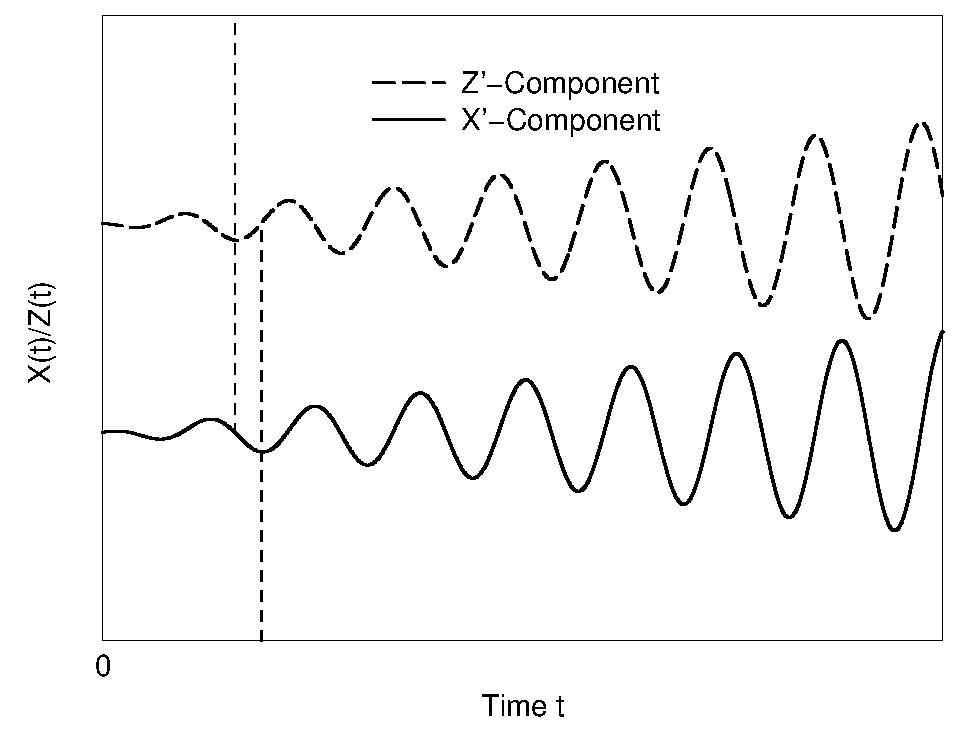
\includegraphics[height=5.5cm]{./figures/XZCoords}
&
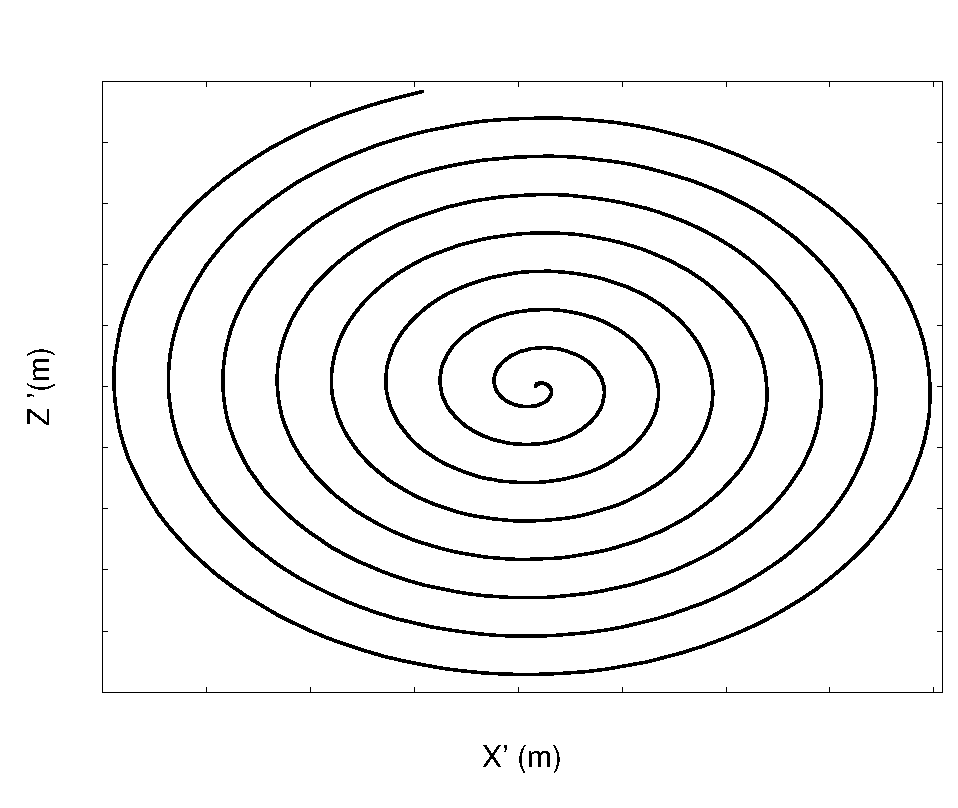
\includegraphics[height=6.5cm,width=5.5cm]{./figures/XZplain}
\end{tabular}
\end{center}
\caption{The x' and z' component as a function of time in the rotating frame (left). A typical neutron trajectory in the rotating frame (right).}
\label{fig:Component}
\end{figure}

Together with the equation for a non-accelerated, linear propagation $\vec{r} = \vec{r_0}+\vec{v}t$ the orthogonal transformation produces a curve in the Z'-X'-plane known as \emph{archidemic spiral}, as can be seen in figure \ref{fig:Component}. The two vector components $s(t) = (z',x')$ follow the equation:
\begin{equation}
s(t) = \left(
\begin{array}{c}
z' \\
x'
\end{array}
\right) = T.\left(
\begin{array}{c}
z(t) \\
x(t)
\end{array}
\right) = \left(
\begin{array}{c}
(z_0+v_z.t)cos(\delta(t)) + (x_0+v_x.t)sin(\delta(t)) \\
-(z_0+v_z.t)sin(\delta(t)) + (x_0+v_x.t)cos(\delta(t))
\end{array}
\right).
\label{eq:Txz}
\end{equation}
For a fixed chopper rotation speed, the neutron trajectory tends to strech from a spiral curve for slow neutrons to a straight line for fast neutrons. For real Fermi chopper settings $\nu$ (about 100 Hz on IN6 at the ILL), neutron trajectories are found to be nearly straight for 1000 m/s neutron velocities \cite{blanc83}.

The basis of the algorithm is to find the intersections of these spiral trajectories with the chopper outer cylinder and then the slit package, in the rotating frame.

For this purpose, the \emph{Ridders's} root finding method was implemented \cite{NumRecip} in order to solve
\begin{equation}
x'(t) = d \textrm{\ or\ } z'(t) = d
\label{eq:Ridder}
\end{equation}
This method provides faster and more accurate intersection determination than other common algorithms. E.g. the secant method fails more often and may give wrong results (outside chopper) whereas the bisection method (a.k.a Picard dichotomy) is slightly slower.

\subsubsection{Standard slit packages (non super-mirror)}

\begin{figure}
\begin{center}
\begin{tabular}{cc}
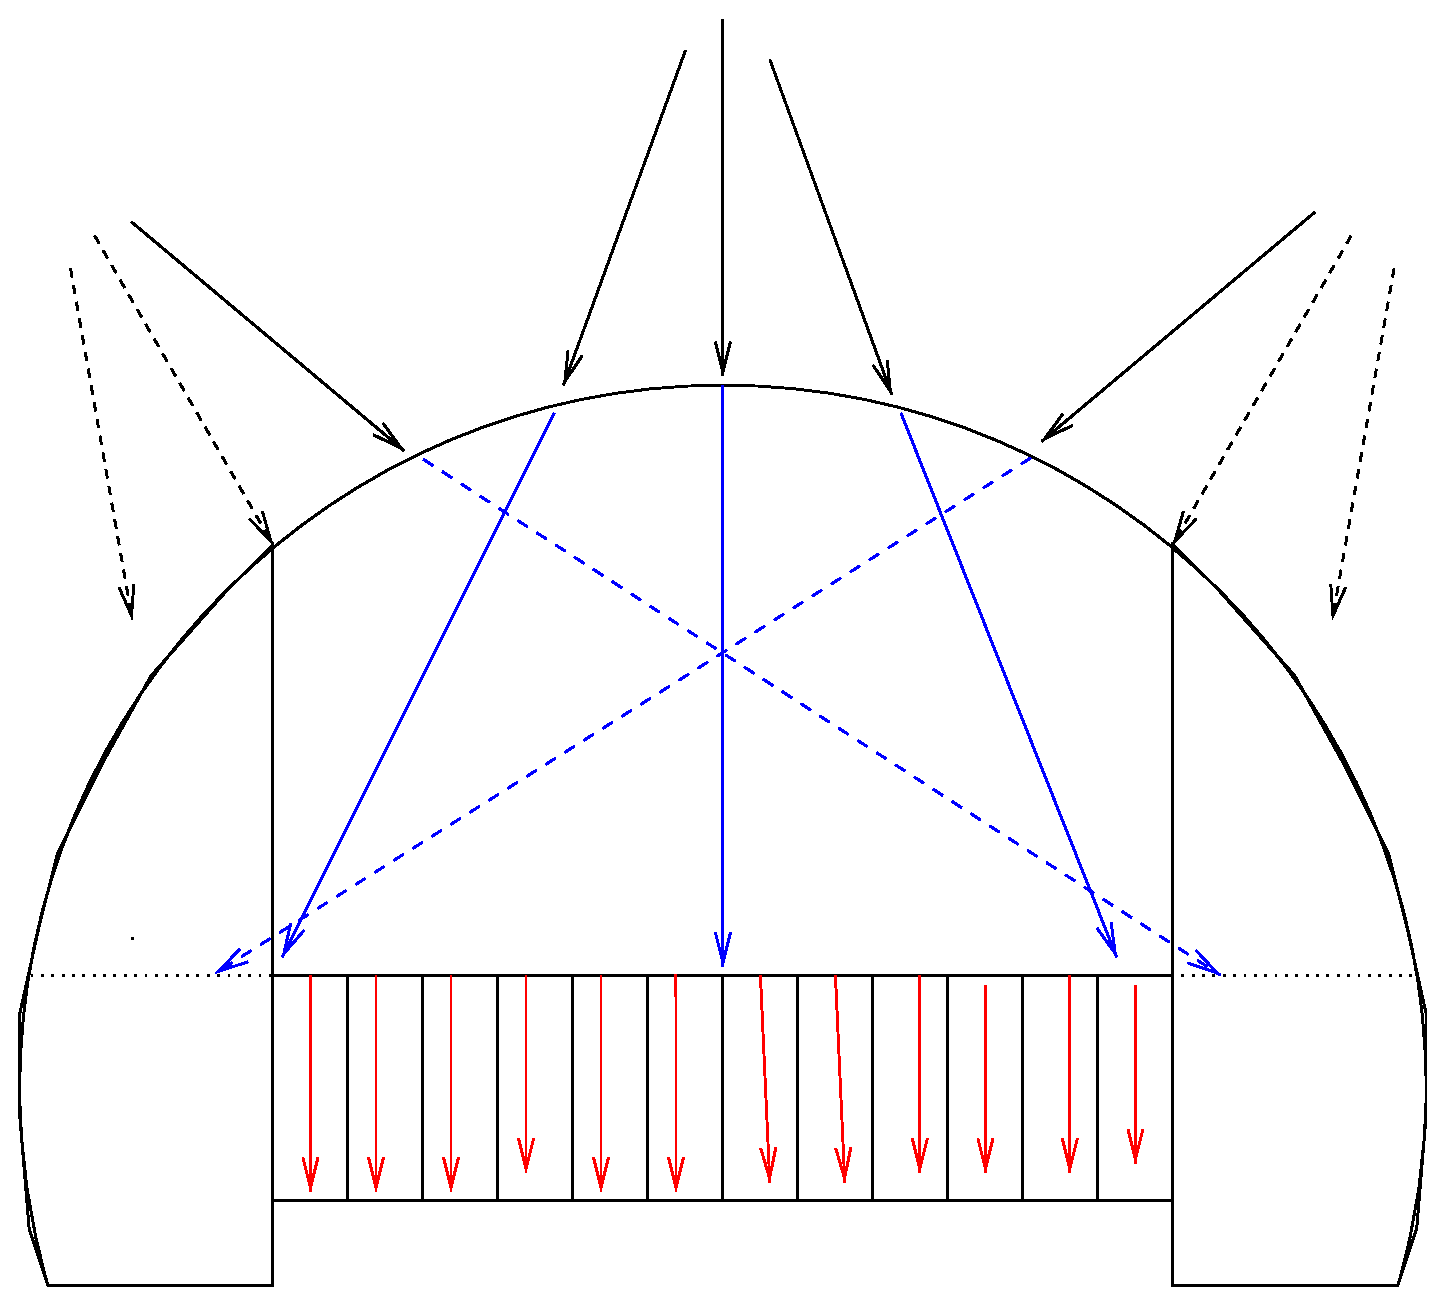
\includegraphics[height=5cm]{./figures/FCAlgo}
&
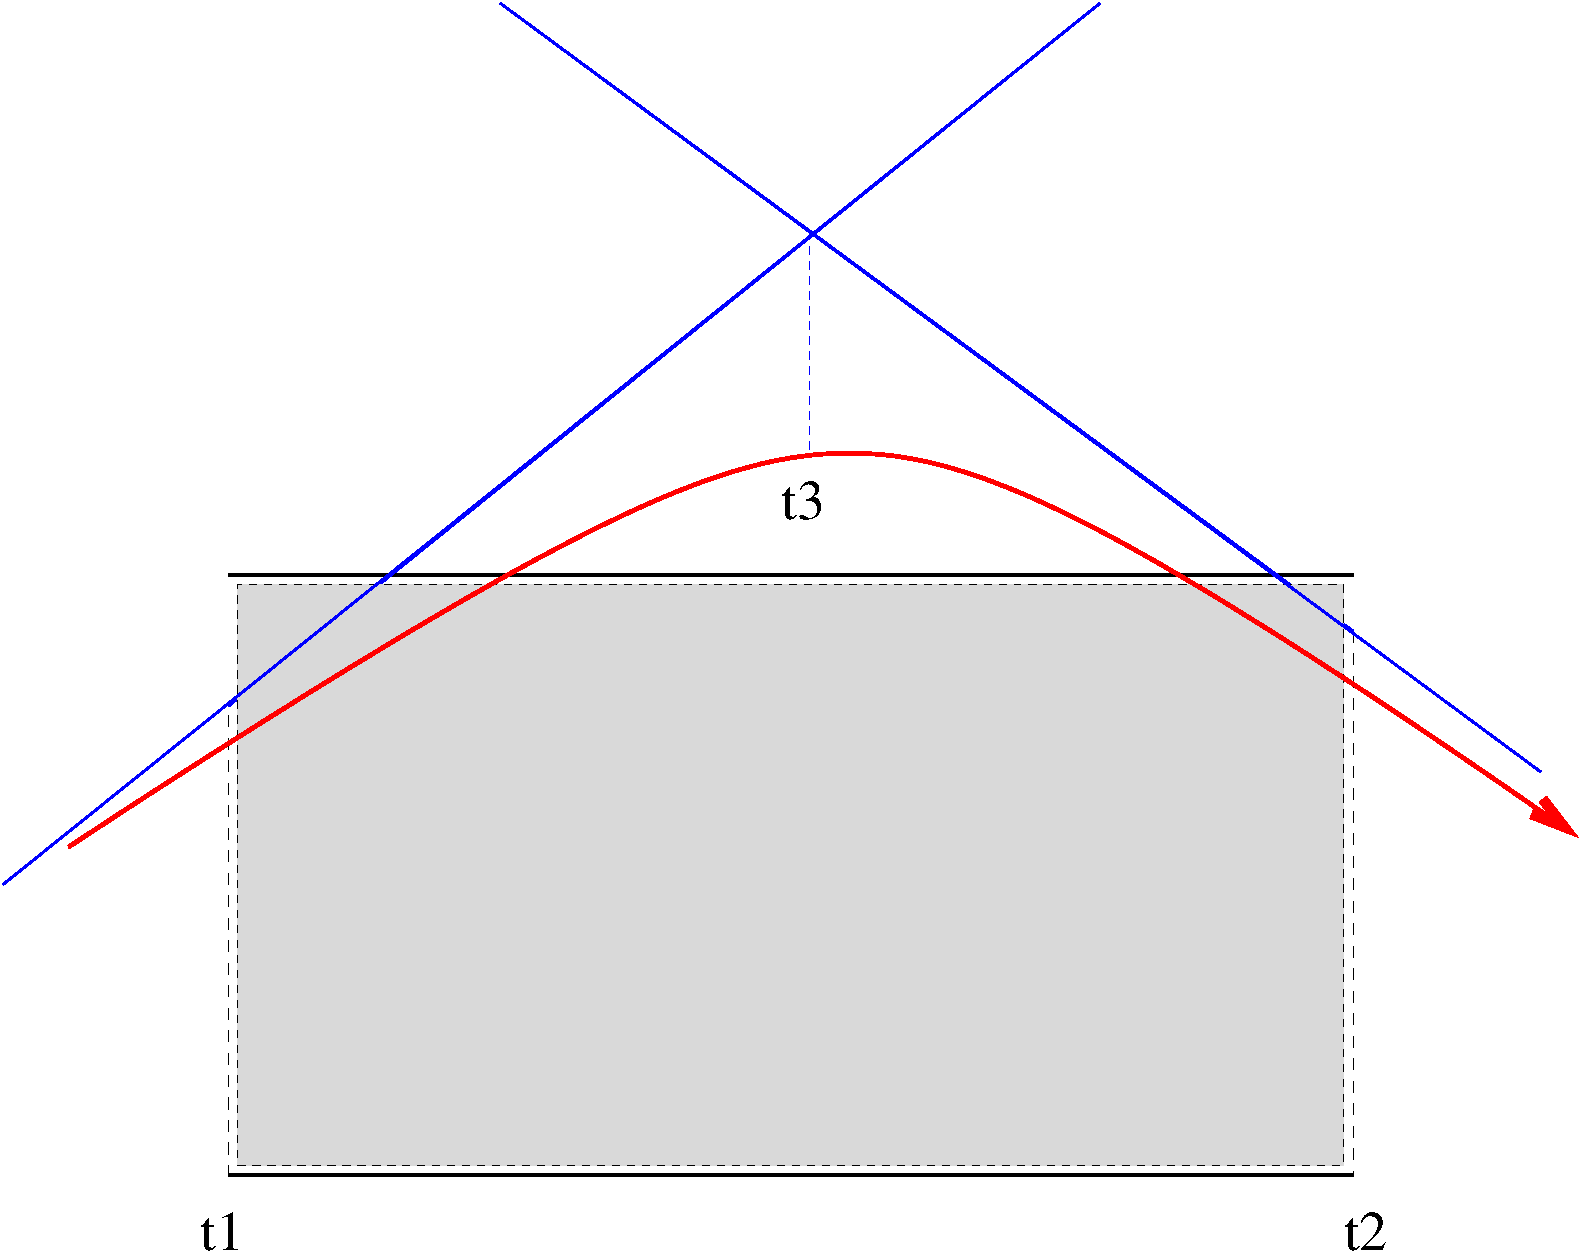
\includegraphics[height=5cm]{./figures/FCtangents}
\end{tabular}
\end{center}
\caption{The different steps in the algorithm (left). A neutron trajectory in a slit (right)}
\label{fig:TOFalg}
\end{figure}

The neutrons are first propagated to the outer chopper cylinder and their coordinates are transformed into the rotating frame using $T$. Neutrons outside the slit channel (chopper opening), or hitting the top and bottom caps are absorbed (yellow dots in Fig. \ref{fig:Overview}). The side from which the neutron approaches the chopper is known (positive or negative z'-axis of the rotating frame) so that the calculation of the time of interaction with the slit package entrance $t_1$ is performed solving $z' = \pm \frac{\textrm{length}}{2}$ in Eq. (\ref{eq:Txz}). Using the result of the numerical algorithms the neutron propagates to the entrance of the slit package (orange circles in Fig. \ref{fig:Overview}). Neutrons getting aside the slit package entrance are absorbed. Additionally, the slit package exit time $t_2$ is estimated the same way with $z' = \mp \frac{\textrm{length}}{2}$, in order to evaluate the whole time-of-flight in the chopper. The index of the slit which was hit is also computed, as we know the $x'$ coordinate in the rotating frame at the slit entrance.

Differentiating Eq. (\ref{eq:Txz}) for $x$ coordinate
\begin{equation}
\dot{x'}(t) = v_x'(t) = [v_x-\omega.(z+v_z.t)]\cos(\omega(t-t_0)) - [v_z+\omega.(x+v_x.t)]\sin(\omega(t-t_0))
\end{equation}
we may estimate the tangents to the spiral neutron trajectory in the rotating frame at times $t_1$ and $t_2$. The intersection of these two lines gives an intermediate time $t_3$.

If the neutron remains in the same slit at this point, then there is no intersection with the slit walls (direct flight), and the neutron may be propagated to the slit output, and then to the cylinder output. A last check is made for the neutron to pass the chopper aperture in the cylinder.

If the neutron changes of slit channel at this point, we may determine the intersection time of the neutron trajectory within $[ t_1, t_3 ]$ or $[ t_3, t_2 ]$, as seen in Fig. \ref{fig:TOFalg}. If walls are not reflecting, we just absorb neutrons here.

\subsubsection{The reflections (super-mirror slits)}

If slit walls are reflecting, neutron is first propagated to the slit separating surface. Then the velocity in the rotating frame is computed using Eq. (\ref{eq:Txz}). Perpendicular velocity $v_x'$ is reverted for reflection, and inverse $T$ transformation is performed. Reflected intensity is computed the same way as for the guide component (see section \ref{s:mirror}). The remaining time $t_2$ to the slit output is estimated and the tangent intersection process is iterated, until neutron exits. Remember that super mirror $m < 1$ parameters behave like $m=1$ materials (see section \ref{ss:mirrorreflect}). Selecting $m=0$ sets the blabes absorbing.

The propagation is finalized when determining the intersection of the neutron trajectory with the outer surface of the chopper cylinder. The neutron must then pass its aperture, else it is absorbed.

\textbf{WARNING:} Issues have been reported for the supermirror slit option in this component. The component works correctly when using the standard, absorbing slits. We will be back with more information during the course of 2017. Meanwhile we suggest to instead use Guide\_channeled with the rotate/derotate option shown in the test instrument Test\_Fermi.instr. 

\subsubsection{Curved slit packages}

The effect of curvature can significantly improve the flux and energy resolution shape.

As all $(zx)$ cordinates are transformed into $(z'x')$, the most efficient way to take into account the curvature is to include it in the transformation Eq. (\ref{eq:Txz}) by 'morphing' the curved rotating real space to a straight still frame. We use parabolic curvature for slits. Then instead of solving
\begin{equation}x'(t) = d - \Delta_{x'}(z') \textrm{\ where\ } \Delta_{x'}(z')=R_{slit}.(1-\sqrt{1-(z'/R_{slit})^2})
\end{equation}
with $\Delta$ being the gap between the straight tangent line at the slit center and the real slit shape, we perform the additional transformation
\begin{equation}
x' \rightarrow x' + \Delta_{x'}(z')
\end{equation}
The additional transformation counter-balances the real curvature so that the rest of the algorithm is written as if slits were straight.
This applies to all computations in the rotating frame, and thus as well to reflections on super mirror coatings.



% Emacs settings: -*-mode: latex; TeX-master: "manual.tex"; -*-

\section{Vitess\_ChopperFermi: The Fermi Chopper from Vitess}
\label{s:vit_fc}
\index{Optics!Fermi Chopper}

%\component{Vitess\_ChopperFermi}{Geza Zsigmond}{GeomOption, $N_{\rm chan}$, $f$, $h$, $w_{\rm tot}$, $l$, $r_{\rm curv}$, $d$, $\phi$, $w_{\rm wall}$, GeomFile}{zerotime, $N_{\rm gates}$}{validated}
\mcdoccomp{optics/Vitess_ChopperFermi.parms}


The component {\bf Vitess\_ChopperFermi} simulates a Fermi chopper with absorbing walls.
The shape of the channels can be straight, curved with circular, or curved with ideal
(i.e. close to a parabolic) shape.
This is determined by the parameter 'GeomOption'. In the option 'straight Fermi
chopper', the very fast neutrons are transmitted with only a time modulation and lower
speed neutrons are modulated both in time of flight and wavelength.
If the channels are curved, the highest transmission occurs for a wavelength

\begin{equation}
\lambda_{\rm opt} = \frac{3956 {\rm [m\AA/s]}}{2 \omega r_{\rm curv}}
\end{equation}

with

\begin{equation}
\omega = 2 \pi f
\end{equation}

The optimal shape is calculated in an exact way and is close to parabolic; in this
case, transmission is as high for the optimal wavelength as in the case of a straight
Fermi chopper for the limit $\lambda \rightarrow 0$.
In the more realistic case of circular shapes channels, the transmission is slightly
lower. In general, neutrons are transmitted through a curved Fermi chopper with a time
AND wavelength modulation .

The rotation axis is vertical (y-axis), i.e. the path length through the channels is
given by the length $l$ along the z-axis. The inital orientation is given by the phase
$\phi$ of the chopper - $\phi$ = 0 means transmission orientation.

Geometry for {\bf straight} and {\bf circular} channels:
The geometry of the chopper consists of a rectangular shaped object with a channel
system. In transmission position, there are $N_{\rm gates}$ slits of width $w_{\rm slit}$
each along the x-axis, separated by absorbing walls of thickness $w_{\rm wall}$
(see figure~\ref{f:vit_fc1}). The total width $w_{\rm tot}$ is given by

\begin{equation}
w_{\rm tot} = N_{\rm gates} w_{\rm slit} + (N_{\rm gates}+1) w_{\rm wall}
\end{equation}

The rectangular channel system is surrounded by a so-called shadowing cylinder; it is a
part of a cylinder with vertical symmetry axis and diameter

\begin{equation}
d \geq \sqrt{l^2 + w_{\rm tot}^2}
\end{equation}

It serves to prevent transmission of neutrons which do not fly through the channels;
but it also reduces the transmission, because the cylinder removes neutrons
in front of the channel entrance or behind the channel exit (see figure~\ref{f:vit_fc1}).

\begin{figure}[ht]
\begin{center}
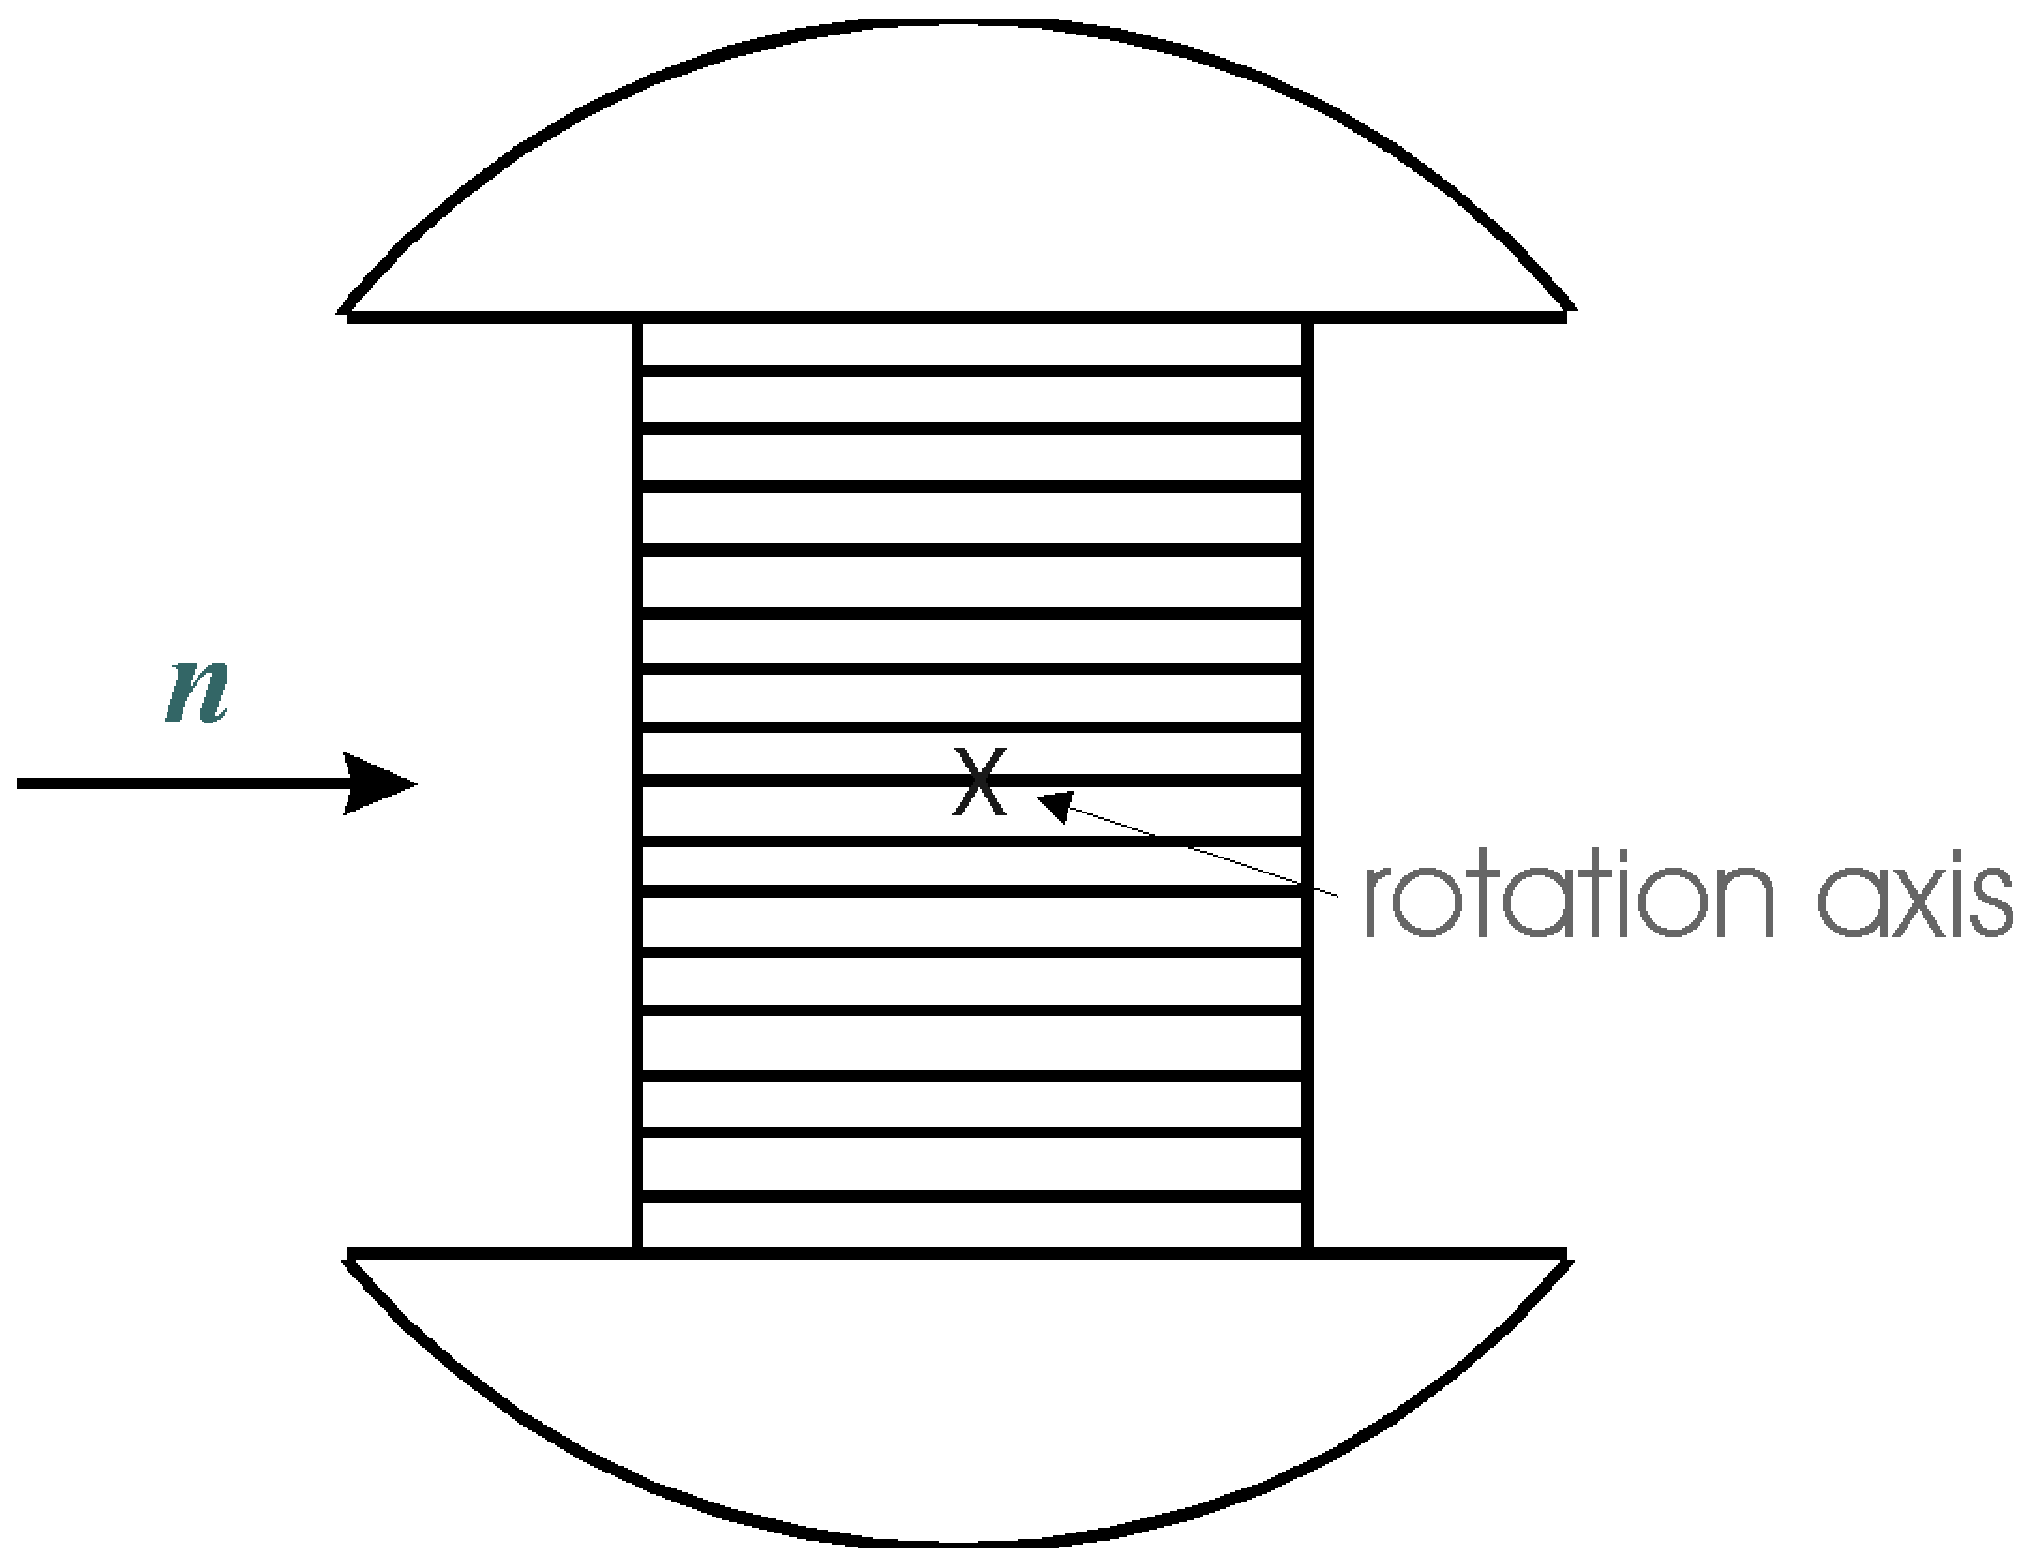
\includegraphics[width=0.45\linewidth]{figures/vitess_fc_str}
\caption{geometry of a staight Fermi chopper\label{f:vit_fc1}}
\end{center}
\end{figure}

Geometry for {\bf parabolic} channels:
In this case, the Fermi chopper is supposed to be a full cylinder, i.e. the central
channels are longer than those on the edges. The other features are the same as for
the other options. (see figure~\ref{f:vit_fc2}).

\begin{figure}[ht]
\begin{center}
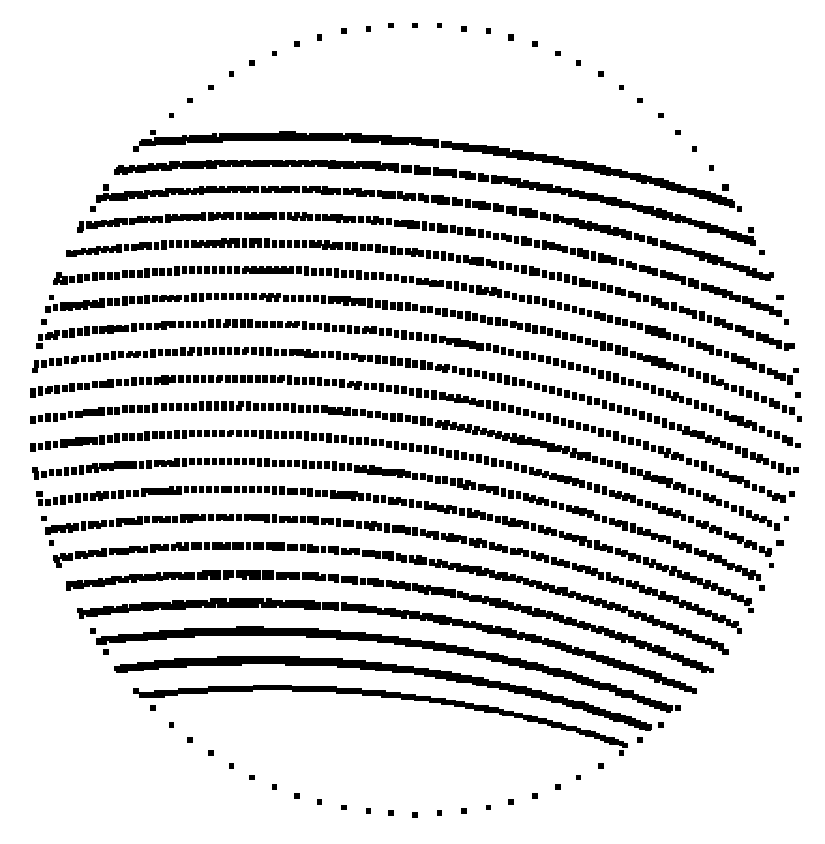
\includegraphics[width=0.4\linewidth]{figures/vitess_fc_parab}
\caption{geometry of a curved Fermi chopper\label{f:vit_fc2}}
\end{center}
\end{figure}

The algorithm works with a rotating chopper framework. Neutrons hitting the channel
walls are absorbed. The channels are approximated by $N_{\rm gates}$ gates. If the trajectory
takes a course through all the gates, the neutron passes the Fermi chopper. There are gates at
the entrance and the exit of the channel. The other gates are situated close to the centre of
the Fermic chopper.
Precision of the simulation increases with the number of gates, but also the computing time needed.
The use of four channels already gives exact transmission shapes for lower wavelengths
($\lambda < 6$ \AA) and good approximation for higher ones. It is recommended to use larger number of
channels only for a check.

The option 'zerotime' may be used to reset the time at the chopper position. The time is
set to a value between -$T_{\rm p}$/2 and +$T_{\rm p}$/2 (with $T_{\rm p}$ being the maximal pulse length),
depending on the phase of the chopper at the moment of passing the chopper centre. The
result is the generation of only 1 pulse instead of several; this is useful for TOF instruments
on continuous sources.

This component is about twice slower than the \verb+FermiChopper+ component.

The component must be placed after a component which sets a non zero flight path to the Fermi Chopper (e.g. not an Arm).


\newpage
\section{V\_selector: A rotating velocity selector}
\label{vselector}
\index{Optics!Velocity selector}

\component{V\_selector}{System}{$L_0$, $L_1$, $\omega$, $r_0$, $\phi$, $N$, height, width}{}{validated, position is center of input aperture}

\begin{figure}
  \begin{center}
    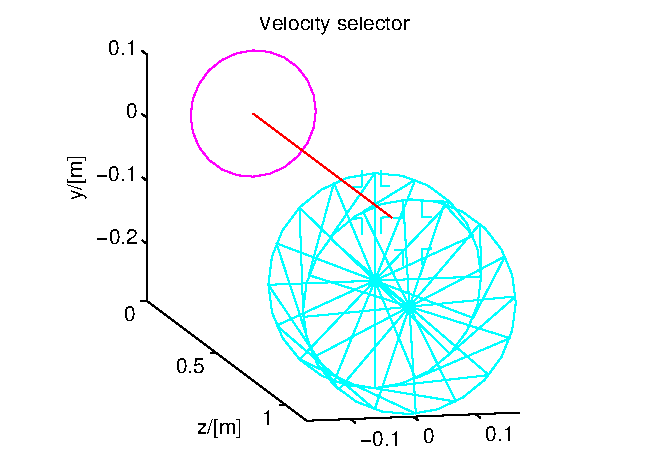
\includegraphics[width=0.9\textwidth]{figures/vselector.eps}
  \end{center}
\caption{A velocity selector}
\label{f:vselector}
\end{figure}

The component {\bf V\_selector} models a rotating velocity
selector constructed from $N$ collimator blades
arranged radially on an axis. Two identical slits ($height \times width$)
at a 12 o'clock position allow
neutron passage at the position of the blades.
The blades are "twisted" on the axis so that a stationary
velocity selector does not transmit neutrons; the total
twist angle is denoted $\phi$ (in degrees).

Further input parameters for {\bf V\_selector} 
the distance between apertures, $L_0$, the length of the
collimator blades, $L_1$, the height from rotation axix to the slit
centre, $r_0$, the rotation speed $\omega$ (in rpm), 
and the blade thickness $t$.

The local coordinate system has its Origo at the slit centre.

The component {\rm Selector} produces equivalent results.

\subsection{Velocity selector transmission}

By rotating the selector you allow
transmittance of neutrons rays with velocities around a nominal value, given by
\begin{equation}
V_0 = \omega L / \phi ,
\end{equation}
which means that the selector has turned the twist angle
$\phi$ during the typical neutron flight time $L/V_0$. The actual twist angle
is $\phi' = \omega t = \omega L / V$.

Neutrons having a velocity slightly different from $V_0$
will either be transmitted or absorbed depending on the exact position
of the rotator blades when the neutron enters the selector.
Assuming this position to be unknown and integrating over all possible
positions (assuming zero thickness of blades), we arrive at a transmission factor
\begin{equation}
T = \left\{
 \begin{array}{ll}
 1 - (N/2\pi ) |\phi-\omega L / V| &
        {\rm if}\;   (N/2\pi )|\phi -\omega L / V| < 1 \\
    0  &  {\rm otherwise}
 \end{array} \right.
\end{equation}
where $N$ is the number of collimator blades.

A horisontal divergence changes the above formula because of the
angular difference between the entry and exit points of the neutron.
The resulting transmittance resembles the one above, only with
$V$ replaced by $V_z$ and $\phi$ replaced by $(\phi +\psi )$,
where $\psi$ is the angular difference due to
the divergence. An additional vertical divergence does not change
this formula, but it may contribute to $\psi$.
(We have here ignored the very small non-linearity of $\psi$ along the
neutron path in case of both vertical and horisontal divergence).

Adding the effect of a finite blade thickness, $t$, reduces the transmission
by the overall factor
\begin{equation}
\left( 1-\frac{N t}{2\pi r}  \right),
\end{equation}
where $r$ is the distance from the rotation axis. We ignore the variation
of $r$ along the neutron path and use just the average value.



\section{Selector: another approach to describe a rotating velocity selector}
\label{selector}
\index{Optics!Velocity selector}

\component{Selector}{System}{$xmin$, $xmax$, $ymin$, $ymax$, $len$, $num$, $width$, $radius$, $\alpha$, $feq$}{}{validated, position is center of input aperture}

The component {\bf Selector} describes the same kind of rotating velocity selector as {\bf V\_selector} - compare
description there - but it uses different parameters and a different algorithm:

The position of the apertures relative to the z-axis (usually the beam centre) is defined by the four parameters
$xmin, xmax, ymin, ymax$. Entry and exit apertures are always identical and situated directly before and behind
the rotor.
There are $num$ blades of thickness $width$ twisted by the angle $\alpha$ (in degrees) on a length $len$.
The selector rotates with a speed $feq$ (in rotation per second); its axle is in a distance $radius$ below the z-axis.

First the neutron is propagated to the entrance window. The loss of neutrons hitting the thin side
of the blades is taken into account by multiplying the neutron weight by a factor

\begin{equation}
   p(r) = \theta_i(r) / \theta_o
\end{equation}

\begin{equation}
   \theta_o = 360^o / num
\end{equation}

$\theta_i$ is the opening between two blades for the distance $r$ between the neutron position (at the entrance)
and the selector axle. The difference between $\theta_o$ and $\theta_i$ is determined by the blade thickness.
The neutron is now propagated to the exit window. If it is outside the regarded channel (between the two actual
blades), it is lost; otherwise it remains in the exit plane.

WARNING - Differences between {\bf Selector} and {\bf V\_selector}:
\begin{itemize}
\item {\bf Selector} has a different coordinate system than {\bf V\_selector};
in {\bf Selector} the origin lies in the entrance plane of the selector.
\item The blades are twisted to the other side, i.e. to the left above the axle in {\bf Selector}.
\item Speed of rotation is given in rotation per second, not in rotations per minute as in {\bf V\_selector}.
\end{itemize}





% there follows a chapter
\newpage
% Emacs settings: -*-mode: latex; TeX-master: "manual.tex"; -*-

\chapter{Monochromators}

In this class of components, we are concerned with elastic Bragg
scattering from monochromators. {\bf Monochromator\_flat}
models a flat thin mosaic crystal with a single scattering vector
perpendicular to the surface.
The component {\bf Monochromator\_curved} is physically similar,
but models a singly or doubly bend monochromator crystal arrangement.

A much more general model of scattering from a single crystal is
found in the component {\bf Single\_crystal},
which is presented under Samples, chapter~\ref{c:samples}.

\section{Monochromator\_flat: An infinitely thin, flat mosaic crystal with
a single scattering vector}
\label{s:monochromator_flat}
\index{Optics!Monochromator}

%\component{Monochromator\_flat}{System}{$z_\textrm{min}$, $z_\textrm{max}$, $y_\textrm{min}$, $y_\textrm{max}$, $\eta_\textrm{h}$, $\eta_\textrm{v}$, $R_0$, $Q_0$}{$d_\textrm{m}$}{In reflecting geometry, non polarized}
\mcdoccomp{optics/Monochromator_flat.parms}

This component simulates an infinitely thin single
crystal with a single scattering vector, $Q_0=2\pi / d_m$, perpendicular to the
surface. A typical
use for this component is to simulate a simple monochromator or analyzer.

The monochromator dimensions are given by the length, $z_\textrm{w}$, and
the height, $y_\textrm{h}$. As the parameter names indicate, the
monochromator is placed in the $z-y$ plane of the local coordinate system.
This definition is made to ensure that the physical monochromator angle
(often denoted \verb+A1+) will equal the \MCS rotation angle
of the Monochromator component around the $y$-axis.
$R_0$ is the maximal reflectivity and
$\eta_\textrm{h}$ and $\eta_\textrm{v}$ are the horizontal and vertical mosaicities,
respectively, see explanation below.

\subsection{Monochromator physics and algorithm}
The physical model used in \textbf{Monochromator\_flat} is a rectangular piece of
material composed of a large number of small micro-crystals.
The orientation of the
micro-crystals deviates from the nominal crystal orientation so that the
probability of a given micro-crystal orientation is proportional to a
Gaussian in the angle between the given and the nominal orientation. The
width of the Gaussian is given by the mosaic spread, $\eta$, of the crystal
(given in units of arc minutes).
$\eta$ is assumed to be large compared to the inherent Bragg width of the
scattering vector (often a few arc seconds).
(The mosaicity gives rise to a Gaussian reflectivity profile of width
similar to - but not equal - the intrinsic mosaicity.
In this component, and in real life, the mosaicity given is that of the
reflectivity signal.)

As a further simplification, the crystal is assumed to be infinitely
thin. This means that multiple scattering effects are not simulated. It
also means that the total reflectivity, $r_0$ is used as a parameter for
the model rather than the atomic scattering cross section, implying that
the scattering efficiency does not vary with neutron wavelength.
The variance
of the lattice spacing ($\Delta d/d$) is assumed to be zero, so this
component is not suitable for simulating backscattering instruments (use
the component \textrm{Single\_crystal}
in section~\ref{s:Single_crystal} for that).

When a neutron trajectory intersects the crystal, the first step in the
computation is to determine the probability of scattering. This
probability is then used in a Monte Carlo choice deciding whether to
scatter or transmit the neutron. The physical scattering probability is the sum
of the probabilities of first- second-, and higher-order scattering -
up to the highest order possible for the given neutron wavelength.
However, in most cases at most one order will have a
significant scattering probability, and the computation thus considers
only the order that best matches the neutron wavelength.

The scattering of neutrons from a crystal is governed by Bragg's law:
\begin{equation}
n\textbf{Q}_0 = 2\textbf{k}_i\sin\theta
\end{equation}
The scattering order is specified by the integer $n$. We seek only one
value of $n$, namely the one which makes
$n \textbf{Q}_0$ closest to the projection of $2\textbf{k}_i$ onto $\textbf{Q}_0$
(see figure~\ref{f:mosaic_order}).
%  k=2PI/lambda
%  q=2k sin(theta)
%
%  2 PI n/k = d q/2k
%  q = n 4 PI/d
%
%  n 2PI/k = n 4 PI/q \sin\theta
%  1/k = 2/q\sin\theta
%  n q = 2k\sin\theta
\begin{figure}
  \begin{center}
    \psfrag{theta}[l][l]{$\theta$}
    \psfrag{ki}[r][r]{$2\textbf{k}_\textrm{i}$}
    \psfrag{Q0}[l][l]{$\textbf{Q}_0$}
    \psfrag{2Q0}[l][l]{$2\textbf{Q}_0$}
    \psfrag{3Q0}[l][l]{$3\textbf{Q}_0$}
    \psfrag{4Q0}[l][l]{$4\textbf{Q}_0$}
    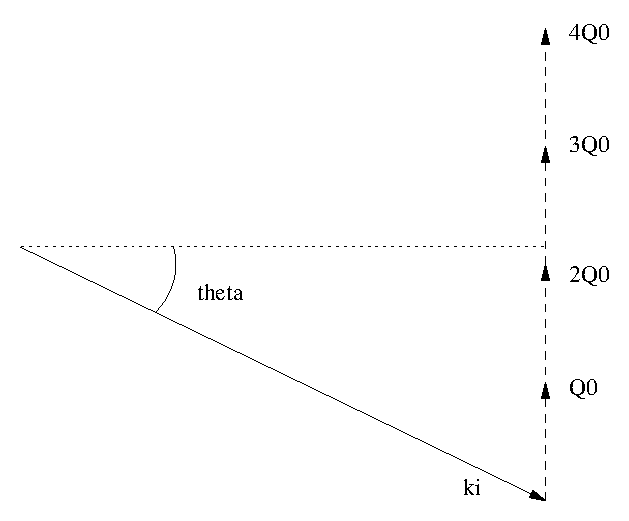
\includegraphics[width=0.5\textwidth]{figures/mosaic_order}
  \end{center}
\caption{Selection of the Bragg order (``2'' in this case).}
\label{f:mosaic_order}
\end{figure}
%

Once $n$ has been determined, the Bragg angle $\theta$ can be
computed. The angle $\alpha$ is the amount one would need to
turn the nominal scattering vector $\textbf{Q}_0$ for the monochromator
to be in Bragg scattering condition.
We now use $\alpha$ to compute the probability of reflection from
the mosaic crystal
\begin{equation}
p_\textrm{reflect} = R_0 e^{-\alpha^2/2\eta^2},
\end{equation}
The probability $p_\textrm{reflect}$ is used
in a Monte Carlo choice to decide whether the neutron is transmitted or
reflected.
%
%\begin{figure}
%  \begin{center}
%    \psfrag{th}[r][r]{$\theta$}
%    \psfrag{ki}[r][r]{$2\textbf{k}_\textrm{i}$}
%    \psfrag{kf}[l][l]{$2\textbf{k}_\textrm{f}$}
%    \psfrag{Q0}[l][l]{$\textbf{Q}_0$}
%    \psfrag{alpha}[c][c]{$\alpha$}
%    \psfrag{q}[l][l]$\textbf{q}$
%    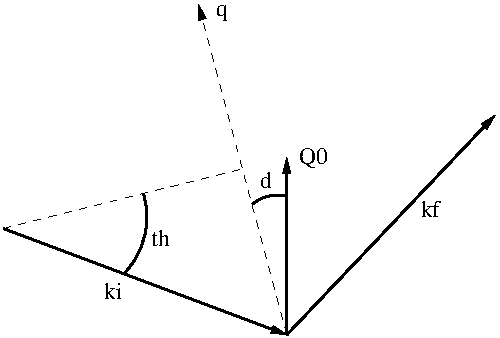
\includegraphics[width=0.5\textwidth]{figures/mosaic_angle}
%  \end{center}
%\caption{Computing the deviation $d$ from the nominal scattering direction.}
%\label{f:mosaic_angle}
%\end{figure}

In the case of reflection, the neutron will be scattered into the
Debye-Scherrer cone, with the probability of each point on the cone
being determined by the mosaic. The Debye-Scherrer cone can be described
by the equation
\begin{equation}
  \label{eq:mosaic_cone}
  \textbf{k}_\textrm{f} = \textbf{k}_\textrm{i}\cos2\theta +
      \sin2\theta(\textbf{c}\cos\varphi + \textbf{b}\sin\varphi),
      \qquad\varphi\in[-\pi;\pi],
\end{equation}
where $\textbf{b}$ is a vector perpendicular to $\textbf{k}_\textrm{i}$ and $\textbf{
Q}_0$, $\textbf{c}$ is perpendicular to $\textbf{k}_\textrm{i}$ and $\textbf{b}$,
and both $\textbf{b}$ and $\textbf{c}$ have the same length as $\textbf{k}_\textrm{i}$
(see figure~\ref{f:mosaic_cone}). When choosing $\varphi$ (and
thereby $\textbf{k}_\textrm{f}$), only a small part of the full $[-\pi; \pi]$
range will have appreciable scattering probability in non-backscattering
configurations. The best statistics is thus obtained by sampling
$\varphi$ only from a suitably narrow range.

The (small) deviation angle $\alpha$ of the nominal
scattering vector $n\textbf{Q}_0$ corresponds to a $\Delta q$ of
\begin{equation}
\Delta q \approx \alpha 2k\sin\theta.
\end{equation}
The angle $\varphi$ corresponds to a $\Delta k_\textrm{f}$ (and hence
$\Delta q$) of
\begin{equation}
\Delta q \approx \varphi k \sin(2\theta)
\end{equation}
(see figure~\ref{f:mosaic_cone}).
Hence we may sample $\varphi$ from a Gaussian with standard deviation
\begin{equation}
\alpha\frac{2k\sin\theta}{k\sin(2\theta)} =
\alpha\frac{2k\sin\theta}{2k\sin\theta\cos\theta} =
\frac{\alpha}{\cos\theta}
\end{equation}
to get good statistics.
%
\begin{figure}
  \begin{center}
    \psfrag{th}[r][r]{$2\theta$}
    \psfrag{ki}[c][c]{$2\textbf{k}_\textrm{i}$}
    \psfrag{kf}[r][r]{$2\textbf{k}_\textrm{f}$}
    \psfrag{nQ0}[l][l]{$n\textbf{Q}_0$}
    \psfrag{q}[l][l]{$\textbf{q}$}
    \psfrag{2ksin2t}[l][l]{$2 k \sin(2 \theta)$}
    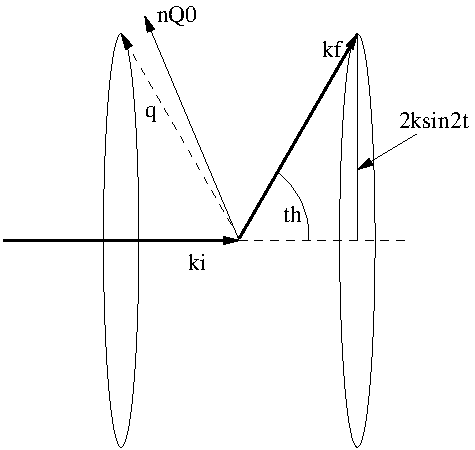
\includegraphics[width=0.5\textwidth]{figures/mosaic_cone}
  \end{center}
\caption{Scattering into the part of the Debye-Scherrer cone covered by
    the mosaic.}
\label{f:mosaic_cone}
\end{figure}

What remains is to determine the neutron weight. The distribution from
which the scattering event is sampled is a Gaussian in $\varphi$ of
width $\frac{\alpha}{\cos\theta}$,
\begin{equation}
    f_\textrm{MC}(\varphi) = \frac{1}{\sqrt{2\pi}(\sigma/\cos\theta)}
            e^{-\varphi^2/2(\sigma/\cos\theta)^2}
\end{equation}
In the physical model, the probability of the scattering event is
proportional to a Gaussian in the angle between the nominal scattering
vector $\textbf{Q}_0$ and the actual scattering vector $\textbf{q}$. The
normalization condition is that the integral over all $\varphi$ should
be 1. Thus the probability of the scattering event in the physical model
is
\begin{equation}
  \label{eq:mosaic_integral}
  \Pi(\varphi) = e^{\frac{-d(\varphi)^2}{2\sigma^2}} /
   \int_{-\pi}^{\pi} e^{\frac{-d(\varphi)^2}{2\sigma^2}} d\varphi
\end{equation}
where $d(\varphi)$ denotes the angle between the nominal scattering
vector and the actual scattering vector corresponding to $\varphi$.
According to equation~(\ref{probrule}), the weight adjustment $\pi_j$ is
then given by
\begin{equation}
\pi_j = \Pi(\varphi) / f_\textrm{MC}(\varphi).
\end{equation}
In the implementation, the integral in~(\ref{eq:mosaic_integral}) is computed
using a 15-order Gaussian quadrature formula, with the integral
restricted to an interval of width $5\sigma/\cos\theta$ for the same
reasons discussed above on the sampling of $\varphi$.


\section{Monochromator\_curved: A curved mosaic crystal with
a single scattering vector}
\label{s:monochromator_curved}
\index{Optics!Monochromator, curved}

%\component{Monochromator\_curved}{(System) Peter Link, FRM-2}{$z_{\rm w}$, $y_{\rm h}$, gap, $\eta_{\rm h}$, $\eta_{\rm v}$, $n_{\rm h}$, $n_{\rm v}$, $R_0$, $Q$, $r_{\rm h}$, $r_{\rm v}$}{$d_{\rm m}$, $\eta$, $h$, $w$, verbose, transmit, reflect}{In reflecting geometry, non polarized}
\mcdoccomp{optics/Monochromator_curved.parms}

\begin{figure}
  \begin{center}
    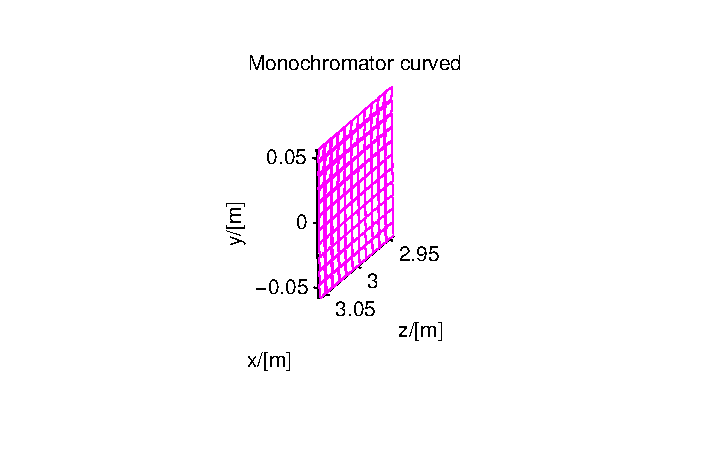
\includegraphics[width=0.9\textwidth]{figures/monochromator_curved}
  \end{center}
\caption{A curved monochromator}
\label{f:monochromator_curved}
\end{figure}


This component simulates an array of infinitely thin single
crystals with a single scattering vector perpendicular to the
surface and a mosaic spread.
This component is used to simulate a singly or doubly
curved monochromator or analyzer in reflecting geometry.

The component uses rectangular pieces of monochromator material
as described in {\bf Monochromator\_curved}.
The scattering vector is named $Q$, and as described in
{\bf Monochromator\_flat}, multiples of $Q$ will be applied.
Other important parameters are the piece height and width,
$y_{\rm h}$ and $z_{\rm w}$, respectively, the
horizontal and vertical mosaicities, $\eta_{\rm h}$ and $\eta_{\rm v}$,
respectively.
If just one mosaicity, $\eta$, is specified, this the same for both directions.

The number of pieces vertically and horizontally are called
$n_{\rm v}$ and $n_{\rm h}$, respectively, and the vertical and horizontal
radii of curvature are named $r_{\rm v}$ and $r_{\rm h}$, respectively.
All single crystals are positioned in the same vertical plane,
but tilted accordingly to the curvature radius.

The constant monochromator reflectivity, $R_0$ can be replaced by
a file of tabulated reflectivities $reflect$ (\verb+*.rfl+ in \verb+MCSTAS/data+). In the same sense, the transmission
can be modeled by a tabulated file $transmit$ (for non-reflected neutrons, \verb+*.trm+ in \verb+MCSTAS/data+).
The most useful of these files for Monochromator\_curved are \verb+HOPG.rlf+ and \verb+HOPG.trm+.

As for {\bf Monochromator\_flat}, the crystal is assumed to be infinitely
thin, and the variation in lattice spacing, ($\Delta d/d$),
is assumed to be zero. Hence, this
component is not suitable for simulating backscattering instruments or to
investigate multiple scattering effects.

The theory and algorithm for scattering from
the individual blades is described under {\bf Monochromator\_flat}.


\section{Single\_crystal: Thick single crystal monochromator plate with multiple scattering}
\index{Optics!Monochromator, thick}

The {\bf Single\_crystal} component may be used to study more complex monochromators, including incoherent scattering, thickness and multiple scattering. Please refer to section \ref{s:Single_crystal}.

\section{Phase space transformer - moving monochromator}
\index{Optics!phase space transformer}

Eventhough there exist a few attempts to write dedicated phase space transformer components, there is an elegant way to put a monochromator into move, by mean of the EXTEND keyword. If you define a SPEED parameter for the instrument, the idea is to change the coordinate system before the monochromator, and restore it afterwards, as follow in the TRACE section:
\begin{lstlisting}
DEFINE INSTRUMENT PST(SPEED=200, ...)
(...)
TRACE
(...)
COMPONENT Mono_PST_on=Arm()
AT ...
EXTEND %{
  vx = vx + SPEED; // monochromator moves transversaly by SPPED m/s
%}

COMPONENT  Mono=Monochromator(...)
AT (0,0,0) RELATIVE PREVIOUS

COMPONENT Mono_PST_off=Arm
AT (0,0,0) RELATIVE PREVIOUS
EXTEND  %{
  vz = vz - SPEED; // puts back neutron in static coordinate frame
%}
\end{lstlisting}
This solution does not contain acceleration, but is far enough for most
studies, and it is very simple. In the latter example, the instance \verb+Mono_PST_on+ should itself be rotated to reflect according to a Bragg law.


\chapter{Samples}
\index{Library!Components!samples}
\index{Samples|textbf}
\label{c:samples}

This class of components models the sample of the experiment.
This is by far the most challenging part of a neutron scattering
instrument to model. However, for purpose of simulating
instrument performance, details of the samples are rather unimportant,
allowing for simple approximations. On the contrary, for full
virtual experiments it is of importance to have realistic and
detailed sample descriptions. \MCS contains both simple and detailed
samples.

We first consider incoherent scattering. The simple component {\bf V-sample}
performs both incoherent scattering and absorption.

An important component class is elastic Bragg scattering from an ideal powder.
The component {\bf PowderN} models a powder scatterer with reflections
given in an input file. To scatter on a single Bragg peak, the {\bf Powder1} component may be used.
The component includes absorption, incoherent scattering, direct beam
transmission and can assume \emph{concentric} shape, i.e. can be used
for modelling sample enviroments.

Next type is Bragg scattering from single crystals.
The simplest single crystals are in fact the monochromator components
like {\bf Monochromator\_flat}, presented in section \ref{s:monochromator_flat}.
The monochromators are models of a thin mosaic crystal
with a single scattering vector perpendicular to the surface.
Much more advanced, the component {\bf Single\_crystal}
is a general single crystal sample (with multiple scattering) that allows
the input of an arbitrary unit cell and a list of structure factors, read
from a LAZY / Crystallographica file.
This component also allows anisotropic mosaicity
and $\Delta d/d$ lattice space variation.

Isotropic small-angle scattering is simulated in {\bf Sans\_Spheres},
which models scattering from a collection of hard spheres (dilute colloids).

Inelastic scattering from a dispersion is exemplified by
the component {\bf Phonon\_simple}, which models
scattering from a single acoustic phonon branch.

For a more general sample model, the {\bf Isotropic\_Sqw} component
is able to simulate all kinds of isotropic materials:
Liquids, glasses, polymers, powders, etc, with $S(q,\omega)$ table
specified by an input file.
Physical processes include coherent/incoherent scattering,
both elastic and inelastic, with absorption and multiple scattering.
Moreover, this component may be used concentrically,
to model a sample environment.
Thus it may handle most samples except single crystals.

\begin{table}
  \begin{center}
  {\let\my=\\
    \begin{tabular}{|c|cc|cc|c|c|}
    \hline
    Sample        & \multicolumn{2}{c|}{Coherent} & \multicolumn{2}{c|}{Incoherent} &&\\
    Process       & Elastic & Inelastic & Elastic & Inelastic & Absorption & Multi. Scatt.\\
    \hline
    Phonon\_simple&         & X         &         &           & 1 & \\
    Isotropic\_Sqw&  X      & X         & X       & X         & 2 & X \\
    Powder1       &  1 line &           & X       &           & 1 & \\
    PowderN       &  N lines&           & X       &           & 1 & \\
    Sans\_spheres &  colloid&           &         &           & 1 & \\
    Single\_crystal& X      &           & X       &           & 2 & X \\
    V\_sample     &         &           & X       & QE broad. & 1 & \\
    Tunneling\_sample &     & X         & X       & QE broad. & 1 & \\
    \hline
    \end{tabular}
    \caption{Processes implemented in sample components. Absorption: 1=single only, 2=with secondary}
    \label{t:sample-process}
  }
  \end{center}
\end{table}
\subsection{Neutron scattering notation}
In sample components, we use the notation common for neutron scattering,
where the wave vector transfer is denoted the {\em scattering vector}
\begin{equation} \label{eq:q-transfer}
{\bf q} \equiv {\bf k}_{\rm i} - {\bf k}_{\rm f} .
\end{equation}
In analygo, the {\em energy transfer} is given by
\begin{equation} \label{eq:w-transfer}
\hbar \omega \equiv E_{\rm i} - E_{\rm f} =
\frac{\hbar^2}{2 m_{\rm n}} \left( k_{\rm i}^2 - k_{\rm f}^2 \right) .
\end{equation}

\subsection{Weight transformation in samples; focusing}

Within many samples,
the incident beam is attenuated by scattering and absorption,
so that the illumination varies considerably throughout the sample.
For single crystals, this phenomenon is known as
{\em secondary extinction} \cite{bacon}, but the effect is
important for all samples.
In analytical treatments, attenuation is difficult to deal with,
and is thus often ignored, making a {\em thin sample approximation}.
In Monte Carlo simulations, the beam attenuation
is easily taken care of, as will be shown below.
In the description, we ignore multiple scattering, which is however
 implemented in some sample components.

The sample has an absorption cross section per unit cell of
$\sigma_c^a$ and a scattering cross section per unit cell
of $\sigma_c^s$. The neutron path length
in the sample before the scattering event is denoted by $l_1$, and
the path length within the sample after the scattering
is denoted by $l_2$, see figure \ref{powderFig}.
We then define the inverse penetration lengths as
$\mu^s = \sigma_c^s / V_c$ and $\mu^a = \sigma_c^a / V_c$, where
$V_c$ is the volume of a unit cell. Physically, the attenuation
along this path follows
\begin{equation}
f_{\rm att}(l) = \exp(- l (\mu^s + \mu^a)) ,
\end{equation}
where the normalization $f_{\rm att}(0)=1$.

\begin{figure}
  \begin{center}
    \psfrag{l1}{$l_1$}
    \psfrag{l2}{$l_2$}
    \psfrag{lfull}{$l_{\rm full}$}
    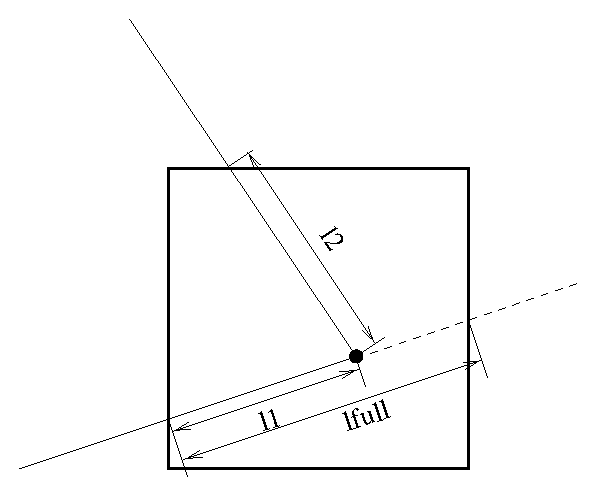
\includegraphics[width=0.6\textwidth]{figures/scatter.eps}
  \end{center}
\caption{The geometry of a scattering event within a powder sample.}
\label{powderFig}
\end{figure}

The probability for a given neutron ray to be scattered from within the interval
$[ l_1 ; l_1+dl ]$ will be
\begin{equation}
P(l_1) dl = \mu^s f_{\rm att}(l_1) dl ,
\end{equation}
while the probability for a neutron to be scattered from within
this interval into the solid angle $\Omega$ {\em and}
not being scattered further
or absorbed on the way out of the sample is
\begin{equation}
P(l_1,\Omega) dl d\Omega =
  \mu^s f_{\rm att}(l_1) f_{\rm att}(l_2) \gamma(\Omega) d\Omega dl ,
\end{equation}
where $\gamma(\Omega)$ is the directional distribution
of the scattered neutrons, and $l_2$ is determined by
Monte Carlo chocies of $l_1$, $\Omega$,
and from the sample geometry, see e.g. figure \ref{powderFig}.

In our Monte-Carlo simulations, we may choose the scattering
parameters by making a Monte-Carlo choice of $l_1$ and $\Omega$
from a distribution different from $P(l_1,\Omega)$.
By doing this, we must adjust $\pi_i$ according to
the probability transformation rule (\ref{probrule}).
If we {\em e.g.}\ choose the scattering depth, $l_1$,
from a flat distribution in $[ 0 ; l_{\rm full} ]$,
and choose the directional dependence from $g(\Omega)$,
we have a Monte Carlo probability
\begin{equation}
f(l_1,\Omega) = g(\Omega) / l_{\rm full} ,
\end{equation}
$l_{\rm full}$ is here the path length through the sample
as taken by a non-scattered neutron (although we here
assume that all simulated neutrons are being scattered).
According to (\ref{probrule}), the neutron weight factor
is now adjusted by the amount
\begin{equation}     \label{sampleprob}
\pi_i(l_1,\Omega) =
 \mu^s l_{\rm full} \exp \left[ - (l_1+l_2) (\mu^a + \mu^s) \right]
  \frac{\gamma(\Omega)}{g(\Omega)} .
\end{equation}

In analogy with the source components, it is possible to define
"interesting" directions for the scattering.
One will then try to focus the scattered neutrons,
choosing a $g(\Omega)$, which peaks around these directions.
To do this, one uses (\ref{sampleprob}), where the
fraction $\gamma(\Omega)/g(\Omega)$ corrects for the focusing.
One must choose a proper distribution so that
$g(\Omega) > 0$ in every interesting direction. If this is not the
case, the Monte Carlo simulation gives incorrect results.
All samples have been constructed with a focusing
and a non-focusing option.


\subsection{Future development of sample components}
There is still room for much more development of functionality in
\MCS samples.

A more general SANS sample is under development.
In addition, a reflectometry sample will soon be developed. In the mean time, you may use the \verb+SiC+ contributed component.

In general, all samples are assumed to be homogeneous. There would also be
potential in developing an inhomogeneous sample, e.g. with
spatially varying lattice constant, relevant for stress/strain scanners.
Inhomogeneously absorbing sample for tomography could also be possible.
Further, no polarization effects are yet taken into account in any
of the samples.


\section{V\_sample: An incoherent scatterer, the V-sample}
\label{s:v_sample}
\index{Samples!Incoherent isotropic scatterer (Vanadium)}
\index{Incoherent elastic scattering}

\component{V\_sample}{System}{$r_{\rm i}$, $r_{\rm o}$, $h$, $r_{\rm foc}$, $x_{\rm target}$, $y_{\rm target}$, $z_{\rm target}$}{$w_x$, $h_y$, $t_z$, $w_{\rm focus}, h_{\rm focus}$, $w_{\rm foc, angle}$, $h_{\rm foc, angle}$, \\ $\sigma_{\rm abs}$, $\sigma_{\rm inc}$, $V_0$, $f_{\rm pack}$, target\_index}{validated}

A sample with incoherent scattering, e.g. vanadium, is frequently used for
calibration purposes, as this gives an isotropic, elastically scattered beam.

The component {\bf V\_sample}
has {\em only} absorption and incoherent elastic scattering.
For the sample geometry, we default use a
hollow cylinder (which has the solid cylinder as a limiting case).
The sample dimensions are: Inner radius $r_{\rm i}$,
outer radius $r_{\rm o}$, and height $h$, see figure \ref{f:v-sample}.
\begin{figure}
  \begin{center}
    \psfrag{ri}{$r_i$}
    \psfrag{ro}{$r_o$}
    \psfrag{h}{$h$}
    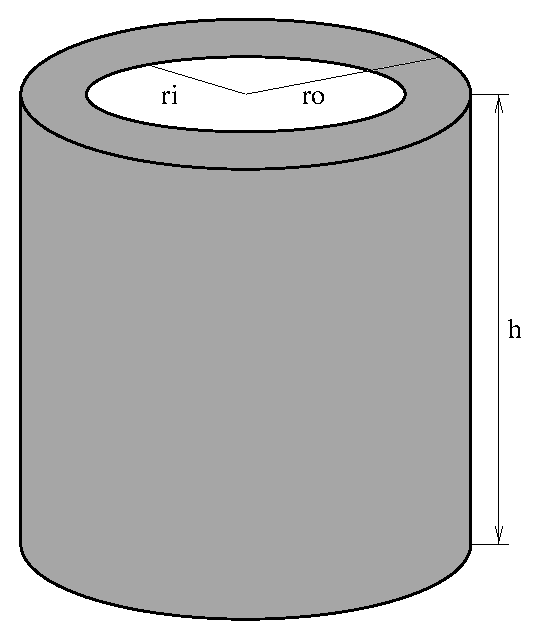
\includegraphics[width=0.3\textwidth]{figures/vsample.eps}
  \end{center}
\caption{The geometry of the hollow-cylinder vanadium sample.}
\label{f:v-sample}
\end{figure}

Alternatively, the sample geometry can be made rectangular
by specifying the width, $w_x$, the height, $h_y$, and the thickness, $t_z$.

The incoherent and absorption cross sections for V are default
for the component. For other choices, the
parameters $\sigma_{\rm inc}$, $\sigma_{\rm abs}$,
and the unit cell volume $V_0$ should be specified.
For a loosely packed sample, also the packing factor, $f_{\rm pack}$
can be specified (default value of 1).

\subsection{Physics and algorithm}

The incoherent scattering gives
a uniform angular distribution of the scattered
neutrons from each nucleus: $\gamma(\Omega) = 1/4\pi$.
For the focusing we choose to have a uniform distribution on
a target sphere of radius $r_{\rm foc}$, at the position
$(x_{\rm target},y_{\rm target},z_{\rm target})$
in the local coordinate system.
This gives an angular distribution (in a small angle approximation)
of
\begin{equation}
g(\Omega) = \frac{1}{4\pi}
  \frac{x_{\rm t}^2+y_{\rm t}^2+z_{\rm t}^2}{(\pi r_{\rm t}^2)}.
\end{equation}

The focusing can alternatively be performed on a rectangle with dimensions
$w_{\rm focus}$, $h_{\rm focus}$, or uniformly in angular space
(in a small-angle approximation),
using $w_{\rm foc, angle}$, $h_{\rm foc, angle}$.
The focusing location can be picked to be a downstream component by
specifying \\
\verb+target_index+.

When calculating the neutron path length within
the cylinder, the kernel function \\
\verb+cylinder_intersect+
is used twice, once for the outer radius and once
for the inner radius.

Multiple scattering is not included in this component. To obtain
intensities similar to real measured ones, we therefore do not
take attenuation from scattering into account for the outgoing
neutron ray.

\subsection{Remark on functionality}
When simulating a realistic incoherent hollow cylinder sample
one finds that  the resulting direction dependence
of the scattered intensity is {\em not} isotropic.
This is explained by the variation of attenuation with
scattering angle.
One test result is shown in the instrument example chapter of the \MCS\ User Manual.

The \verb+Samples_vanadium+ and \verb+Samples_incoherent+ test/example instruments exist in the distribution for this component.
         \newpage
\section{Tunneling\_sample: An incoherent inelastic scatterer}
\label{s:Tunneling_sample}
\index{Samples!Incoherent inelastic scatterer}
\index{Incoherent inelastic scattering}

\component{Tunneling\_sample}{System}{$r_{\rm i}$, $r_{\rm o}$, $h$, $r_{\rm foc}$, $x_{\rm target}$, $y_{\rm target}$, $z_{\rm target}$}{$w_x$, $h_y$, $t_z$, $w_{\rm focus}, h_{\rm focus}$, $w_{\rm foc, angle}$, $h_{\rm foc, angle}$, $\sigma_{\rm abs}$, $\sigma_{\rm inc}$, $V_0$, $f_{\rm pack}$, $f_{\rm QE}$, $f_{\rm tun}$, $\Gamma$, $E_{\rm tun}$, target\_index}{not validated}

The component {\bf Tunneling\_sample}
displays incoherent inelastic scattering as found in a number of systems, {\em e.g.}
containing mobile hydrogen. 

For the sample geometry, we default use a
hollow cylinder (which has the solid cylinder as a limiting case).
The sample dimensions are: Inner radius $r_{\rm i}$,
outer radius $r_{\rm o}$, and height $h$. This geometry is the same as 
the default for {\bf V\_sample}, see figure \ref{f:v-sample}.

As for {\bf V\_sample}, the sample geometry can be made rectangular 
by specifying the width, $w_x$, the height, $h_y$, and the thickness, $t_z$.

Also the focusing properties are the same as for {\bf V\_sample}.
For the focusing is performed as a uniform distribution on
a target sphere of radius $r_{\rm foc}$, at the position
$(x_{\rm target},y_{\rm target},z_{\rm target})$
in the local coordinate system.
The focusing can alternatively be performed on a rectangle with dimensions
$w_{\rm focus}$, $h_{\rm focus}$, or uniformly in angular space
(in a small-angle approximation),
using $w_{\rm foc, angle}$, $h_{\rm foc, angle}$.
The focusing location can be picked to be a downstream component by
specifying \verb+target_index+.

The incoherent and absorption cross sections for V are default
for the component. For other choices, the
parameters $\sigma_{\rm inc}$, $\sigma_{\rm abs}$,
and the unit cell volume $V_0$ should be specified.
For a loosely packed sample, also the packing factor, $f_{\rm pack}$
can be specified (default value of 1).

The inelastic scattering takes place as a quasielastic (Lorentzian)
component, which is chosen with probability $f_{\rm QE}$.
The broadening of the signal is given by $\Gamma$ (HWHM).
In addition, a tunneling signal is present with a probability of $f_{\rm tun}$ 
and a tunneling energy of $\pm E_{\rm tun}$. 
The tunneling peaks are weighted by the usual factor $k_{\rm f}/k_{\rm i}$.

The total scattering cross section is given by
\begin{eqnarray}
\lefteqn{\frac{d^2\sigma}{d\Omega dE_{\rm f}}(q,\omega) = \frac{\sigma_{\rm inc}}{4\pi}
\times \left\{ (1-f_{\rm QE}-f_{\rm inel}) \delta(\hbar \omega) \right. }  \\
 &+& f_{\rm QE} \frac{\Gamma}{(\hbar\omega)^2+\Gamma^2}
 + \left.\frac{f_{\rm inel}}{2} \frac{k_{\rm f}}{f_{\rm i}} 
   \left[\delta(\hbar\omega-E_{\rm tun}) + \delta(\hbar\omega+E_{\rm tun}) \right] \right\} \nonumber
\end{eqnarray}

The component takes care that 
$f_{\rm QE} + f_{\rm tun} \leq 1$, otherwise an error is returned.

The component accounts for absorption, 
but not multiple scattering. To obtain
intensities similar to real measured ones, we therefore do not 
take attenuation from scattering into account for the outgoing
neutron ray.

        \newpage
\section{PowderN: A general powder sample}
\index{Samples!Powder, multiple diffraction line}
\index{Diffraction}
\index{Sample environments}
\index{Concentric components}
\label{powder}

\component{Powder\_N}{System}{$radius$, $thickness$, $h$, $xwidth$, $yheight$, $zdepth$, $\sigma_{\rm abs}$,
  $\sigma_{\rm inc}$, $Vc$, $f_{\rm pack}$, reflections, format, DW, concentic, and more}{}{}

The powder diffraction component {\bf PowderN} models a powder sample
with background coming only from incoherent scattering and no
multiple scattering. At the users choice, a given percentage of the incoming
events may be transmitted (attenuated) to model the direct beam. The component can also
assume \emph{concentric} shape, i.e. be used for describing sample environment (cryostat,
sample container etc.). 

The description of the powder comes from a file in one of the standard output formats LAZY, FULLPROF, or CRYSTALLOGRAPHICA.

A usage example of this component can be found in the \\
\verb+Neutron site/Tutorial/templateDIFF+ instrument from the \verb+mcgui+.

\subsection{Files formats: powder structures}

Data files of type \verb'lau' and \verb'laz' in the \MCS distribution data directory are self-documented in their header. A list of common powder definition files is available in Table \ref{t:powders-data} (page \pageref{t:powders-data}). They do not need any additional parameters to be used, as in the example:
\begin{lstlisting}
  PowderN(<geometry parameters>, filename="Al.laz")
\end{lstlisting}
Other column-based file formats may also be imported e.g. with parameters such as:
\begin{lstlisting}
  format=Crystallographica
  format=Fullprof
  format={1,2,3,4,0,0,0,0}
\end{lstlisting}
In the latter case, the indices define order of columns parameters
multiplicity, lattice spacing, $F^2$, Debye-Waller factor and intrinsic line width.

The column signification may as well explicitely be set in the data file header using any of the lines:
\begin{lstlisting}
  #column_j     <index of the multiplicity 'j' column>
  #column_d     <index of the d-spacing 'd' column>
  #column_F2    <index of the squared str. factor '|F|^2' column [b]>
  #column_F     <index of the structure factor norm '|F|' column>
  #column_DW    <index of the Debye-Waller factor 'DW' column>
  #column_Dd    <index of the relative line width Delta_d/d 'Dd' column>
  #column_inv2d <index of the 1/2d=sin(theta)/lambda 'inv2d' column>
  #column_q     <index of the scattering wavevector 'q' column>
\end{lstlisting}

Other component parameters may as well be specified in the data file
header with lines e.g.:
\begin{lstlisting}
  #V_rho        <value of atom number density [at/Angs^3]>
  #Vc           <value of unit cell volume Vc [Angs^3]>
  #sigma_abs    <value of Absorption cross section [barns]>
  #sigma_inc    <value of Incoherent cross section [barns]>
  #Debye_Waller <value of Debye-Waller factor DW>
  #Delta_d/d    <value of Detla_d/d width for all lines>
  #density      <value of material density [g/cm^3]>
  #weight       <value of material molar weight [g/mol]>
  #nb_atoms     <value of number of atoms per unit cell>
\end{lstlisting}

Further details on file formats are available in the \verb+mcdoc+ page
of the component.

\subsection{Geometry, physical properties, concentricity}
The sample has the shape of a solid cylinder, radius $r$ and height $h$ or a box-shaped
sample of size $xwidth$ x $yheight$ x $zdepth$. At the users choice, an inner 'hollow' can be
specified using the parameter $thickness$. 


As the Isotropic\_Sqw component~\ref{s:isotropic-sqw}, PowderN assumes \emph{concentric} shape, i.e.
can contain other components inside the inner hollow. To allow this, two almost identical copies
of the PowderN components must be set up \emph{around} the internal component(s), for example:


\begin{lstlisting}
COMPONENT Cryo = PowderN(reflections="Al.laz", radius = 0.01, thickness = 0.001,
                          concentric = 1)
AT (0,0,0) RELATIVE Somewhere

COMPONENT Sample = some_other_component(with geometry FULLY enclosed in the hollow)
AT (0,0,0) RELATIVE Somewhere

COMPONENT Cryo2 = COPY(Cryo)(concentric = 0)
AT (0,0,0) RELATIVE Somewhere
\end{lstlisting}

As outlined, the first instance of PowderN \emph{must} have \verb+concentric = 1+ and the instance \emph{must}
have \verb+concentric = 0+. Furthermore, the component(s) inside the hollow \emph{must} have a geometry which can
be fully contained inside the hollow.


In addition to the coherent scattering specified in the \verb+reflections+ file, absorption- and incoherent 
cross sections can be given using the input parameters $\sigma_c^a$ and $\sigma_i^s$.


The Bragg scattering from the powder,
$\sigma_c^s$ is calculated from the input file, with the parameters
$Q$, $|F(Q)|^2$, and $j$ for the scattering vector, structure factor, and
multiplicity, respectively. The volume of the unit cell is denoted $Vc$,
while the sample packing factor is $f_{\rm pack}$.


%Further, the incoherent scattering is only taken into account
%by the attenuation of the beam, given by (\ref{e:attenu})
%and $\sigma_c^a$.
%The incoherently scattered neutrons are not
%propagated through to the detector, but rather not generated at all.

Focusing is performed by only scattering into one angular
interval, $d\phi$ of the Debye-Scherrer circle. The center of this
interval is located at the point where the Debye-Scherrer circle
intersects the half-plane defined by the initial velocity, ${\bf v}_{\rm i}$,
and a user-specified vector, {\bf f}.

%The input parameters for this component are
%
%\begin{lstlisting}\begin{tabular}{ccl}
%$r$ & m & Radius of cylinder \\
%$h$ & m & Height of cylinder \\
%$\sigma_c^a$ & fm$^2$ & Absorption cross section per unit cell (at 2200 m/s) \\
%$\sigma_{i,c}^s$ & (fm)$^2$ & Incoherent scattering cross section per unit cell \\
%$\rho'/\rho$ & 1 & Packing factor \\
%$V_c$ & \AA$^3$ & Volume of unit cell \\
%${\bf Q}$ & \AA$^{-1}$ & The reciprocal lattice vector under consideration \\
%$|F({\bf Q}_j)|^2$ & (fm)$^2$ &
% Structure factor \\
%$j$ & 1 & Multiplicity of reflection \\
%$\exp(-2W)$ & 1 & Debye-Waller factor \\
%$d\phi$ & deg & Angular interval of focusing \\
%$f_x$ & m & \\
%$f_y$ & m & Focusing vector\\
%$f_z$ & m & \\
%\end{tabular}\end{lstlisting}

\subsection{Powder scattering}
An ideal powder sample consists of many small
crystallites, although each crystallite is sufficiently
large not to cause measurable size broadening.
The orientation of the crystallites is evenly distributed,
and there is thus always a large number of
crystallites oriented to fulfill the Bragg condition
\begin{equation}   \label{Bragg}
n \lambda = 2 d \sin \theta ,
\end{equation}
where $n$ is the order of the scattering (an integer), $\lambda$
is the neutron wavelength, $d$ is the lattice spacing of the sample,
and $2 \theta$ is the scattering angle, see figure \ref{coneFig}.
As all crystal orientations
are realised in a powder sample, the neutrons are scattered within a
{\em Debye-Scherrer cone} of opening angle $4 \theta$ \cite{bacon}.

\begin{figure}
  \begin{center}
    \psfrag{2theta}[c][c]{$2\theta$}
    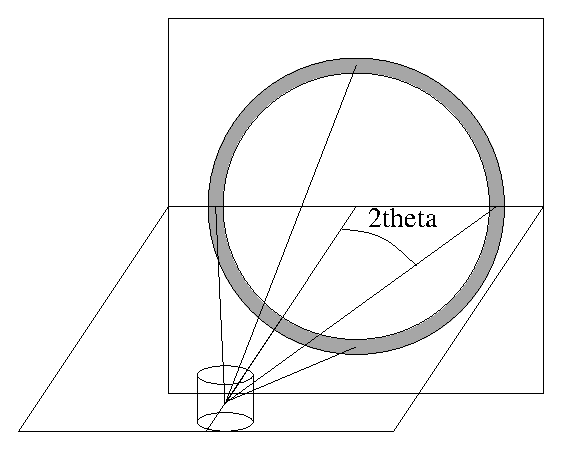
\includegraphics[width=0.6\textwidth]{figures/powder}
  \end{center}
\caption{The scattering geometry of a powder sample showing part of the
Debye-Scherrer cone (solid lines) and the Debye-Scherrer circle (grey).}
\label{coneFig}
\end{figure}

Equation (\ref{Bragg}) may be cast into the form
\begin{equation}
|{\bf Q}| = 2 |{\bf k}| \sin \theta ,
\end{equation}
where {\bf Q} is a vector of the reciprocal lattice, and {\bf k} is
the wave vector of the neutron. It is seen that only
reciprocal vectors fulfilling $|{\bf Q}| < 2 |{\bf k}|$
contribute to the scattering.
For a complete treatment of the powder sample, one needs to take
into account all these {\bf Q}-values, since each of them contribute
to the attenuation.

The strength of the Bragg reflections is given by their structure factors
\begin{equation}
 \left| \sum_j b_j \exp({\bf R}_j \cdot {\bf Q}) \right|^2 ,
\end{equation}
where the sum runs over all atoms in one unit cell. This structure factor is
non-zero only when $Q$ equals a reciprocal lattice vector.

The textbook expression for the scattering cross section
corresponding to one Debye-Scherrer cone reads \cite[ch.3.6]{squires}, with $V=N V_0$ being the total sample volume:
\begin{equation}
\sigma_{\rm cone}
  = \frac{V}{V_0^2} \frac{\lambda^3}{4 \sin \theta} \sum_Q |F(Q)|^2 .
\end{equation}
For our purpose, this expression should be changed slightly.
Firstly, the sum over structure factors for a particular $Q$ is replaced
by the sum over essentially different reflections multiplied by their
multiplicity, $j$. Then, a finite packing factor, $f$, is defined for the powder,
and finally, the Debye-Waller factor is multiplied on the elastic cross section
to take lattice vibrations into account (no inelastic background is simulated,
however). We then reach
\begin{eqnarray}
\sigma_{\rm cone, Q}
 & = & j_Q f \exp(-2W) \frac{V}{V_0^2} \frac{\lambda^3}{4 \sin \theta} |F(Q)|^2 \\
 & = & f \exp(-2W) \frac{N}{V_0} \frac{4\pi^3}{k^2} \frac{j_Q |F(Q)|^2}{Q}
\end{eqnarray}
in the thin sample approximation. For samples of finite thickness, the
beam is being attenuated by the attenuation coefficient
\begin{equation}
\label{e:attenu}
\mu_{\rm Q} = \sigma_{\rm cone,Q} / V .
\end{equation}
For calibration it may be useful to consider the total intensity
scattered into a detector of effective height $h$, covering only
one reflection \cite[ch.3.6]{squires}.
A cut though the Debye-Scherrer cone perpendicular to its axis
is a circle. At the distance $r$ from the sample, the radius of this
circle is $r \sin(2\theta)$. Thus, the detector (in a small angle
approximation) counts a fraction $h / (2 \pi r \sin(2 \theta))$
of the scattered neutrons, giving a resulting count intensity:
\begin{equation}
I = \Psi \sigma_{\rm cone,Q} \frac{h}{2 \pi r \sin(2\theta)} ,
\end{equation}
where $\Psi$ is the flux at the sample position.

For clarity we repeat the meaning and unit of the symbols:
%
\begin{lstlisting}
\begin{tabular}{ccl}
$\Psi$ & s$^{-1}$m$^{-2}$ & Incoming intensity of neutrons \\
$I$    & s$^{-1}$ & Detected intensity of neutrons \\
$h$    & m        & Height of detector \\
$r$    & m        & Distance from sample to detector \\
$f$    & 1        & Packing factor of the powder \\
$j$    & 1        & Multiplicity of the reflection \\
$V_0$  & m$^{3}$  & Volume of unit cell\\
$|F({\bf Q})|^2$ & m$^2$  & Structure factor \\
$\exp(-2W)$ & 1  & Debye-Waller factor \\
$\mu_{\rm Q}$ & m$^{-1}$ & Linear attenuation factor due to scattering from
one powder line. \\
\end{tabular}
\end{lstlisting}
%
%Often, one defines the {\em scattering power} as
%\begin{equation}
%Q \equiv N^2 \frac{|F({\bf Q})|^2 \lambda^3}{V \sin(2\theta)}
% = N_c^2 V \frac{\rho'}{\rho} \frac{|F({\bf Q})|^2 \lambda^3}{\sin(2\theta)} ,
%\end{equation}
%where $N$ is the number of unit cells.

A powder sample will in general have several allowed reflections
${\bf Q}_j$, which will all contribute to the attenuation.
These reflections will have different values of
$|F({\bf Q}_j)|^2$ (and hence of $Q_j$), $j_j$, $\exp(-2W_j)$,
and $\theta_j$.
The total attenuation through the sample due to scattering is given by
$\mu^s = \mu_{\rm inc}^s + \sum_j \mu^s_j $,
where $\mu_{\rm inc}^s$ represents the incoherent scattering.

\subsection{Algorithm}
The algorithm of {\bf PowderN} can be summarized as
\begin{itemize}
\item Check if the neutron ray intersects the sample (otherwise ignore
the following).
\item Calculate the attenuation coefficients for scattering and absorption.
\item Perform Monte Carlo choices to determine the scattering position,
scattering type (coherent/incoherent), and the outgoing direction.
\item Perform the necessary weight factor transformation.
\end{itemize}

%\subsection{Calculating the weight factor}
          \newpage
\section{Single\_crystal: The single crystal component}
\label{s:Single_crystal}
\index{Samples!Single crystal diffraction}
\index{Diffraction}
\index{Incoherent elastic scattering}
\index{Multiple scattering}

\component{Single\_crystal}{Kristian Nielsen}{$x_{width}, y_{height}, z_{thick}$,$\vec a, \vec b, \vec c, \Delta d/d$, mosaic, reflections}{$\sigma_{abs}, \sigma_{inc}$, ...}{Partially validated, centered. Further validation undergoing. Known BUGS: The component is known not to work as a Bragg monochromator, likely the problem relates to the internal definition of the reciprocal space. Possibly related to this, the model of anistropic mosaic is broken - always use a non-zero isotropic mosaic. Also, always use a non-zero value of the $\Delta d/d$ parameter.}

The {\bf Single\_crystal} component models a thick, flat single crystal
with multiple scattering and absorption with elastic coherent scattering.
An elastic incoherent background may also be simulated.
It may be used to describe samples for diffraction,
but also for accurate monochromator descriptions.
The component is currently under further review. The current documentation is outdated, especially with respect to the model of crystal mosaicity.

The input parameters for the component are \textit{xwidth},
\textit{yheight}, and \textit{zdepth} to define the dimensions of the
crystal in meters (area is centered); \textit{delta\_d\_d} to give the
value of $\Delta d/d$ (no unit);
$(\textit{ax}, \textit{ay}, \textit{az})$, $(\textit{bx}, \textit{by},
\textit{bz})$, and $(\textit{cx}, \textit{cy}, \textit{cz})$ to define
the axes of the direct lattice of the crystal (the sides of the unit
cell) in units of {\AA}ngstr{\o}m; and \textit{reflections}, a string
giving the name of the file with the list of structure factors to
consider.
The mosaic is specified \emph{either} isotropically as
\textit{mosaic}, \emph{or} anisotropically as \textit{mosaic\_h}
(rotation around the $Y$ axis), \textit{mosaic\_v} (rotation around the
$Z$ axis), and \textit{mosaic\_n} (rotation around the $X$ axis); in all
cases in units of full-width-half-maximum minutes of arc.

Optionally, the absorption cross-section at 2200 m/s and the incoherent
cross-section may be given as \textit{absorption} and
\textit{incoherent} (in barns), with default of zero; and
\textit{p\_transmit} may be assigned a fixed Monte Carlo probability for
transmission through the crystal without any interaction.

The user must specify a list of reciprocal lattice vectors
$\boldsymbol{\tau}$ to consider along with their structure factors
$|F_{\boldsymbol{\tau}}|^2$. The user must also specify the coordinates
(in direct space) of the unit cell axes $\boldsymbol{a}$,
$\boldsymbol{b}$, and $\boldsymbol{c}$, from which the reciprocal lattice
will be computed. See section \ref{s:Single_crystal_implement} for file format specifications.

In addition to coherent scattering, {\bf Single\_crystal} also
handles incoherent scattering and absorption. The incoherent scattering
cross-section is supplied by the user as a constant
$\sigma_{\rm inc}$. The absorption cross-section is supplied by the user at
2200~m/s, so the actual cross-section for a neutron of velocity $v$ is
$\sigma_{\rm abs} = \sigma_{2200} \frac{\rm 2200~m/s}{v}$.

\subsection{The physical model}

The textbook expression for the scattering cross-section of a crystal
is~\cite[ch.3]{squires}:
\begin{equation}
\label{eq:sigma_coh_el}
\left(\frac{d\sigma}{d\Omega}\right)_{\rm coh.el.} =
        N\frac{(2\pi)^3}{V_0}\sum_{\boldsymbol{\tau}}
        \delta(\boldsymbol{\tau} - \boldsymbol{\kappa})|F_{\boldsymbol{\tau}}|^2
\end{equation}
Here $|F_{\boldsymbol{\tau}}|^2$ is the structure factor
(defined in section~\ref{powder}), $N$ is the
number of unit cells, $V_0$ is the volume of an
individual unit cell, and $\boldsymbol{\kappa} (= {\bf k}_i - {\bf k}_f)$
is the scattering vector. $\delta(\boldsymbol{x})$ is a 3-dimensional delta
function in reciprocal space,
so for given incoming wave vector ${\bf k}_i$ and lattice vector
${\boldsymbol{\tau}}$, only a single final wave vector ${\bf k}_f$ is allowed.
In general, this wavevector will not fulfill the conditions for elastic
scattering $(k_f = k_i)$.
In a real crystal, however, reflections are not perfectly sharp. Because
of imperfection and finite-size effects, there will be a small region
around $\boldsymbol{\tau}$ in reciprocal space of possible scattering vectors.

{\bf Single\_crystal} simulates a crystal with a mosaic spread
$\eta$ and a lattice plane spacing uncertainty $\Delta d/d$. In such
crystals the reflections will not be completely sharp;
there will be a small region around each reciprocal lattice point of the
crystal that contains valid scattering vectors.

We model the mosaicity and $\Delta d/d$ of the crystal with
3-dimensional Gaussian functions in reciprocal space (see
figure~\ref{fig:crystal-reciprocal-space}). Two of the axes of the
Gaussian are perpendicular to the reciprocal lattice vector $\boldsymbol{\tau}$ and model
the mosaicity. The third one is parallel to $\boldsymbol{\tau}$ and models
$\Delta d/d$. We assume that the
mosaicity is small so that the possible directions of the scattering
vector may be approximated with a Gaussian in rectangular
coordinates.
\begin{figure}[t]
  \begin{center}
    \psfrag{ki}[r][r]{$\boldsymbol{k}_{\rm i}$}
    \psfrag{kf}[l][l]{$\boldsymbol{k}_{\rm f}$}
    \psfrag{tau}[r][r]{$\boldsymbol{\tau}$}
    \psfrag{mosaic}[l][l]{$\eta$}
    \psfrag{del-d-d}[l][l]{$\Delta d/d$}
    \psfrag{Ewald}[l][l]{Ewald}
    \psfrag{Sphere}[l][l]{Sphere}
    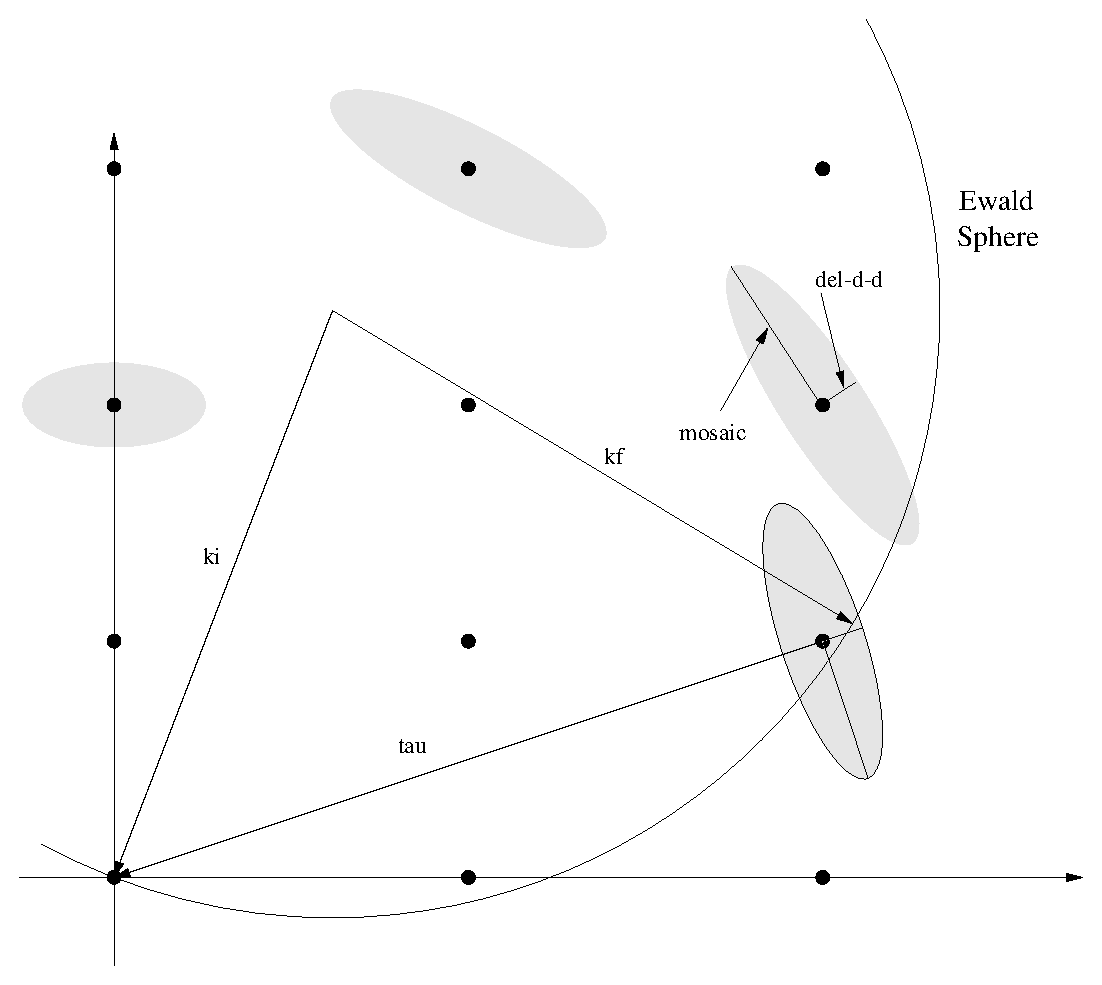
\includegraphics[width=0.7\textwidth]{figures/recip_space3.eps}
  \end{center}
\caption{Ewald sphere construction for a single neutron showing the
    Gaussian broadening of reciprocal lattice points in their local
    coordinate system.}
\label{fig:crystal-reciprocal-space}
\end{figure}

If the mosaic is isotropic (the same in all directions), the two
Gaussian axes perpendicular to $\boldsymbol{\tau}$ are simply arbitrary
normal vectors of equal length given by the mosaic. But if the mosaic
is anisotropic, the two perpendicular axes will in general be different
for each scattering vector. In the absence of anything better,
{\bf Single\_crystal} uses a model which is at least mathematically
plausible and which works as expected in the two common cases:
(1)~isotropic mosaic, and (2)~two mosaic directions (``horizontal and
vertical mosaic'') perpendicular to a scattering vector.

The basis for the model is a three-dimensional Gaussian distribution in
Euler angles giving the orientation probability distribution for the
micro-crystals; that is, the misorientation is given by small rotations
around the $X$, $Y$, and $Z$ axes, with the rotation angles having (in
general different) Gaussian probability distributions. For given
scattering vector $\boldsymbol{\tau}$, a rotation of the micro-crystals
around an axis parallel to $\boldsymbol{\tau}$ has no effect on the
direction of the scattering vector. Suppose we form the intersection
between the three-dimensional Gaussian in Euler angles and a plane
through the origin perpendicular to $\boldsymbol{\tau}$. This gives a
two-dimensional Gaussian, say with axes defined by unit vectors
$\boldsymbol{g}_1$ and $\boldsymbol{g}_2$ and mosaic widths $\eta_1$ and
$\eta_2$.

We now let the mosaic for $\boldsymbol{\tau}$ be defined by rotations
around $\boldsymbol{g}_1$ and $\boldsymbol{g}_2$ with angles having
Gaussian distributions of widths $\eta_1$ and $\eta_2$. Since
$\boldsymbol{g}_1$, $\boldsymbol{g}_2$, and $\boldsymbol{\tau}$ are
perpendicular, a small rotation of $\boldsymbol{\tau}$ around
$\boldsymbol{g}_1$ will change $\boldsymbol{\tau}$ in the direction of
$\boldsymbol{g}_2$. The two axes of the Gaussian mosaic in reciprocal
space that are perpendicular to $\boldsymbol{\tau}$ will thus be given
by $\tau\eta_2\boldsymbol{g}_1$ and $\tau\eta_1\boldsymbol{g}_2$.

We now derive a quantitative expression for the scattering cross-section
of the crystal in the model. For this, we introduce a \emph{local
  coordinate system} for each reciprocal lattice point
$\boldsymbol{\tau}$ and use $\boldsymbol{x}$ for vectors written in local
coordinates. The origin is $\boldsymbol{\tau}$, the first axis
is parallel to $\boldsymbol{\tau}$ and the other two axes are
perpendicular to $\boldsymbol{\tau}$. In the local coordinate system,
the 3-dimensional Gaussian is given by
\begin{equation}
  \label{eq:crystal-gauss-1}
  G(x_1,x_2,x_3) = \frac{1}{(\sqrt{2\pi})^3}\frac{1}{\sigma_1\sigma_2\sigma_3}
  e^{-\frac{1}{2}(\frac{x_1^2}{\sigma_1^2} +
  \frac{x_2^2}{\sigma_2^2} + \frac{x_3^2}{\sigma_3^2})}
\end{equation}
The axes of the Gaussian are $\sigma_1 = \tau\Delta d/d$ and $\sigma_2 =
\sigma_3 = \eta\tau$. Here we used the assumption that $\eta$ is small,
so that $\tan\eta \approx \eta$ (with $\eta$ given in radians).  By
introducing the diagonal matrix
$$
D = \left(
  \begin{array}[c]{ccc}
    \frac{1}{2}\sigma_1^2 & 0 & 0 \\
    0 & \frac{1}{2}\sigma_2^2 & 0 \\
    0 & 0 & \frac{1}{2}\sigma_3^2
  \end{array}\right)
$$
equation~(\ref{eq:crystal-gauss-1}) can be written as
\begin{equation}
  G(\boldsymbol{x}) =
  \frac{1}{(\sqrt{2\pi})^3}\frac{1}{\sigma_1\sigma_2\sigma_3}
  e^{-\boldsymbol{x}^{\rm T} D \boldsymbol{x}}
\end{equation}
again with $\boldsymbol{x}=(x_1,x_2,x_3)$ written in local coordinates.

To get an expression in the coordinates of the reciprocal lattice of the
crystal, we introduce a matrix $U$ such that if $\boldsymbol{y} =
(y_1,y_2,y_3)$ are the global coordinates of a point in the crystal
reciprocal lattice, then $U(\boldsymbol{y} + \boldsymbol{\tau})$ are the
coordinates in the local coordinate system for $\boldsymbol{\tau}$. The
matrix $U$ is given by
$$ U^{\rm T} = (\hat{u}_1, \hat{u}_2, \hat{u}_3), $$
where $\hat{u}_1$, $\hat{u}_2$, and $\hat{u}_3$ are the axes of the
local coordinate system, written in the global coordinates of the
reciprocal lattice. Thus
$\hat{u}_1 = \boldsymbol{\tau}/\tau$,  and $\hat{u}_2$ and $\hat{u}_3$ are
unit vectors perpendicular to $\hat{u}_1$ and to each other.
The matrix $U$ is unitarian, that is
$U^{-1} = U^{\rm T}$. The translation between global and local
coordinates is
$$ \boldsymbol{x} = U(\boldsymbol{y} + \boldsymbol{\tau}) \qquad
   \boldsymbol{y} = U^{\rm T} \boldsymbol{x} - \boldsymbol{\tau} $$

The expression for the 3-dimensional Gaussian in global coordinates is
\begin{equation}
  G(\boldsymbol{y}) =
  \frac{1}{(\sqrt{2\pi})^3}\frac{1}{\sigma_1\sigma_2\sigma_3}
  e^{-(U(\boldsymbol{y}+\boldsymbol{\tau}))^{\rm T} D (U(\boldsymbol{y}+\boldsymbol{\tau}))}
\end{equation}
The elastic coherent cross-section is then given by
\begin{equation}
  \label{eq:crystal-cross-section}
  \left(\frac{d\sigma}{d\Omega}\right)_{\rm coh.el.} =
        N\frac{(2\pi)^3}{V_0}\sum_{\boldsymbol{\tau}}
        G(\boldsymbol{\tau} - \boldsymbol{\kappa})
         |F_{\boldsymbol{\tau}}|^2
\end{equation}

\subsection{The algorithm}

The overview of the algorithm used in the Single\_crystal component is
as follows:
\begin{enumerate}
\item\label{enum:crystal-1} Check if the neutron intersects the
  crystal. If not, no action is taken.
\item\label{enum:crystal-2} Search through a list of reciprocal lattice
  points of interest, selecting those that are close enough to the Ewald
  sphere to have a non-vanishing scattering probability. From these,
  compute the total coherent cross-section $\sigma_{\rm coh}$ (see
  below), the absorption cross-section $\sigma_{\rm abs} = \sigma_{\rm
  2200} \frac{{\rm 2200~m/s}}{v}$, and the total cross-section
  $\sigma_{\rm tot} = \sigma_{\rm coh}+\sigma_{\rm inc}+\sigma_{\rm abs}$.
\item\label{enum:crystal-3} The transmission probability is
  $\exp(- \frac{\sigma_{\rm tot}}{V_0}\ell)$ where $\ell$ is the length of
  the flight path through the crystal. A Monte Carlo choice is
  performed to determine
  whether the neutron is transmitted. Optionally, the user may
  set a fixed Monte Carlo probability for the first scattering event,
  for example to boost the statistics for a weak reflection.
\item\label{enum:crystal-4} For non-transmission, the position at which
  the neutron will interact is selected from an exponential
  distribution. A Monte Carlo choice is made of whether to scatter
  coherently or incoherently. Absorption is treated by weight adjustment
  (see below).
\item\label{enum:crystal-5} For incoherent scattering, the outgoing wave
  vector $\boldsymbol{k}_{\rm f}$ is selected with a random direction.
\item\label{enum:crystal-6} For coherent scattering, a reciprocal
  lattice vector is selected by a Monte Carlo choice, and
  $\boldsymbol{k}_{\rm f}$ is found (see below).
\item\label{enum:crystal-7} Adjust the neutron weight as dictated by the
  Monte Carlo choices made.
\item\label{enum:crystal-8} Repeat from~(\ref{enum:crystal-2}) until the
  neutron is transmitted (to simulate multiple scattering).
\end{enumerate}

For point~\ref{enum:crystal-2}, the distance
\textit{dist} between a reciprocal lattice point and the Ewald sphere is
considered small enough to allow scattering if it is less than five
times the maximum axis of the Gaussian, $\textit{dist} \leq
5\max(\sigma_1,\sigma_2,\sigma_3)$.

\subsection{Choosing the outgoing wave vector}

The final wave vector $\boldsymbol{k}_{\rm f}$ must lie on the
intersection between the Ewald sphere and the Gaussian ellipsoid. Since
$\eta$ and $\Delta d/d$ are assumed small, the intersection can be
approximated with a plane tangential to the sphere, see
figure~\ref{fig:crystal-scattering-tri}. The tangential point is taken
to lie on the line between the center of the Ewald sphere
$-\boldsymbol{k}_{\rm i}$ and the reciprocal lattice point
$\boldsymbol{\tau}$. Since the radius of the Ewald sphere is $k_{\rm
  i}$, this point is
$$ \boldsymbol{o}=(k_{\rm i}/\rho - 1)\boldsymbol{\rho} - \boldsymbol{\tau} $$
where $\boldsymbol{\rho} = \boldsymbol{k}_{\rm i} - \boldsymbol{\tau}$.
\begin{figure}[t]
  \begin{center}
    \psfrag{ki}[r][r]{$\boldsymbol{k}_{\rm i}$}
    \psfrag{kf}[l][l]{$\boldsymbol{k}_{\rm f}$}
    \psfrag{rho}[r][r]{$\boldsymbol{\rho}$}
    \psfrag{tau}[r][r]{$\boldsymbol{\tau}$}
    \psfrag{x}[l][l]{$\boldsymbol{x}$}
    \psfrag{Ewald}[r][r]{Ewald}
    \psfrag{Sphere}[r][r]{Sphere}
    \psfrag{Tangential}[l][l]{Tangential}
    \psfrag{plane}[l][l]{plane}
    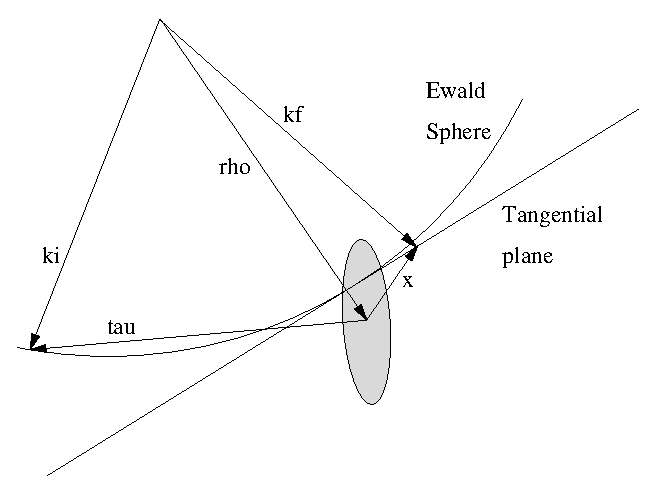
\includegraphics[width=0.7\textwidth]{figures/recip-detail.eps}
  \end{center}
\caption{The scattering triangle in the single crystal.}
\label{fig:crystal-scattering-tri}
\end{figure}

The equation for the plane is
\begin{equation}
  \label{eq:crystal-tangent-plane}
    \boldsymbol{P}(\boldsymbol{t}) = \boldsymbol{o} + B \boldsymbol{t}, \qquad
    \boldsymbol{t} \in \mathbb{R}^2
\end{equation}
Here $B = (\boldsymbol{b}_1, \boldsymbol{b}_2)$ is a $3\times 2$ matrix
with the two generators for the plane $\boldsymbol{b}_1$ and
$\boldsymbol{b}_2$. These are (arbitrary) unit vectors in the plane,
being perpendicular to
each other and to the plane normal $\boldsymbol{n} =
\boldsymbol{\rho}/\rho$.

Each $\boldsymbol{t}$ defines a potential final wave vector
$\boldsymbol{k}_{\rm f}(\boldsymbol{t}) = \boldsymbol{k}_{\rm i} +
\boldsymbol{P}(\boldsymbol{t})$. The value of the 3-dimensional Gaussian
for this $\boldsymbol{k}_{\rm f}$ is
\begin{equation}
  \label{eq:crystal-gauss-t-1}
  G(\boldsymbol{x}(\boldsymbol{t})) =
  \frac{1}{(\sqrt{2\pi})^3}\frac{1}{\sigma_1\sigma_2\sigma_3}
  e^{-\boldsymbol{x}(\boldsymbol{t})^{\rm T} D \boldsymbol{x}(\boldsymbol{t})}
\end{equation}
where $\boldsymbol{x}(\boldsymbol{t}) = \boldsymbol{\tau} -
(\boldsymbol{k}_{\rm i} - \boldsymbol{k}_{\rm f}(\boldsymbol{t}))$ is
given in local coordinates for $\boldsymbol{\tau}$. It can be shown that
equation~(\ref{eq:crystal-gauss-t-1}) can be re-written as
\begin{equation}
  \label{eq:crystal-gauss-2}
  G(\boldsymbol{x}(\boldsymbol{t})) =
  \frac{1}{(\sqrt{2\pi})^3}\frac{1}{\sigma_1\sigma_2\sigma_3} e^{-\alpha}
  e^{-(\boldsymbol{t}-\boldsymbol{t}_0)^{\rm T} M
    (\boldsymbol{t}-\boldsymbol{t}_0)}
\end{equation}
where $M = B^{\rm T} D B$ is a $2 \times 2$ symmetric and positive
definite matrix, $\boldsymbol{t}_0 = -M^{-1}B^{\rm T} D \boldsymbol{o}$
is a 2-vector, and $\alpha = -\boldsymbol{t}_0^{\rm T} M
\boldsymbol{t}_0 + \boldsymbol{o}^{\rm T} D \boldsymbol{o}$ is a real
number.  Note that this is a two-dimensional Gaussian (not necessarily
normalized) in $\boldsymbol{t}$ with center $\boldsymbol{t}_0$ and axis
defined by $M$.

To choose $\boldsymbol{k}_{\rm f}$ we sample $\boldsymbol{t}$ from the
2-dimensional Gaussian distribution~(\ref{eq:crystal-gauss-2}). To do
this, we first construct the Cholesky decomposition of the matrix
$(\frac{1}{2}M^{-1})$. This gives a $2\times 2$ matrix $L$ such that $L
L^{\rm T} = \frac{1}{2}M^{-1}$ and is possible since $M$ is symmetric
and positive definite. It is given by
$$
  L = \left(
  \begin{array}[c]{cc}
    \sqrt{\nu_{11}} & 0 \\
    \frac{\nu_{12}}{\sqrt{\nu_{11}}} & \sqrt{\nu_{22} - \frac{\nu_{12}^2}{\nu_{11}}}
  \end{array}\right)
\qquad\hbox{where }
  \frac{1}{2}M^{-1} = \left(
  \begin{array}[c]{cc}
    \nu_{11} & \nu_{12} \\
    \nu_{12} & \nu_{22}
  \end{array}\right)
$$
Now let $\boldsymbol{g} = (g_1, g_2)$ be two random numbers drawn form a
Gaussian distribution with mean 0 and standard deviation 1, and let
$\boldsymbol{t} = L\boldsymbol{g} + \boldsymbol{t}_0$. The probability
of a particular $\boldsymbol{t}$ is then
\begin{eqnarray}
  P(\boldsymbol{t})d\boldsymbol{t}
    &=& \frac{1}{2\pi}
      e^{-\frac{1}{2}\boldsymbol{g}^{\rm T}\boldsymbol{g}} d\boldsymbol{g} \\
    &=& \frac{1}{2\pi}\frac{1}{\det L}
      e^{-\frac{1}{2}(L^{-1}(\boldsymbol{t}-\boldsymbol{t}_0))^{\rm T}
          (L^{-1}(\boldsymbol{t}-\boldsymbol{t}_0))} d\boldsymbol{t} \\
    &=& \frac{1}{2\pi}\frac{1}{\det L}
      e^{-(\boldsymbol{t}-\boldsymbol{t}_0)^{\rm T}
          M(\boldsymbol{t}-\boldsymbol{t}_0)} d\boldsymbol{t}
  \label{eq:crystal-gauss-prob-1}
\end{eqnarray}
where we used that
$\boldsymbol{g}=L^{-1}(\boldsymbol{t}-\boldsymbol{t}_0)$ so that
$d\boldsymbol{g} = \frac{1}{\det L}d\boldsymbol{t}$. This is just the
normalized form of~(\ref{eq:crystal-gauss-2}). Finally we set
$\boldsymbol{k}'_{\rm f} = \boldsymbol{k}_{\rm i} +
\boldsymbol{P}(\boldsymbol{t})$ and
$\boldsymbol{k}_{\rm f} = (k_{\rm i}/k'_f)\boldsymbol{k}'_{\rm f}$ to
normalize the length of $\boldsymbol{k}_{\rm f}$ to correct for the
(small) error introduced by approximating the Ewald sphere with a plane.

\subsection{Computing the total coherent cross-section}

To determine the total coherent scattering cross-section, the differential
cross-section must be integrated over the Ewald sphere:
$$
\sigma_{\rm coh} = \int_{\rm Ewald}
\left(\frac{d\sigma}{d\Omega}\right)_{\rm coh.el.} d\Omega
$$
For small mosaic we may approximate the sphere with the tangential
plane, and we thus get from~(\ref{eq:crystal-cross-section})
and~(\ref{eq:crystal-gauss-2}):
\begin{eqnarray}
  \label{eq:crystal-coh-cs}
  \sigma_{{\rm coh},\boldsymbol{\tau}} &=& \int N\frac{(2\pi)^3}{V_0}
        G(\boldsymbol{\tau} - \boldsymbol{\kappa})
         |F_{\boldsymbol{\tau}}|^2 d\Omega \\
  &=& \frac{1}{\boldsymbol{k}_i^2} N\frac{(2\pi)^3}{V_0}
         \frac{1}{(\sqrt{2\pi})^3}\frac{e^{-\alpha}}{\sigma_1\sigma_2\sigma_3}
         |F_{\boldsymbol{\tau}}|^2
         \int e^{-(\boldsymbol{t}-\boldsymbol{t}_0)^{\rm T} M
         (\boldsymbol{t}-\boldsymbol{t}_0)}
         d\boldsymbol{t} \\
  &=& \det(L) \frac{1}{\boldsymbol{k}_i^2} N\frac{(2\pi)^{3/2}}{V_0}
         \frac{e^{-\alpha}}{\sigma_1\sigma_2\sigma_3}
         |F_{\boldsymbol{\tau}}|^2
         \int e^{-\frac{1}{2}\boldsymbol{g}^{\rm T}\boldsymbol{g}}
         d\boldsymbol{g} \\
  &=& 2\pi\det(L) \frac{1}{\boldsymbol{k}_i^2} N\frac{(2\pi)^{3/2}}{V_0}
         \frac{e^{-\alpha}}{\sigma_1\sigma_2\sigma_3}
         |F_{\boldsymbol{\tau}}|^2 \\
  &=& \frac{\det(L)}{\boldsymbol{k}_i^2} N\frac{(2\pi)^{5/2}}{V_0}
         \frac{e^{-\alpha}}{\sigma_1\sigma_2\sigma_3}
         |F_{\boldsymbol{\tau}}|^2 \\
  \sigma_{\rm coh} &=& \sum_{\boldsymbol{\tau}} \sigma_{{\rm coh},\boldsymbol{\tau}}
\end{eqnarray}
As before, we let $\boldsymbol{g} = L^{-1}(\boldsymbol{t} -
\boldsymbol{t}_0)$ so that $d\boldsymbol{t} = \det(L) d\boldsymbol{g}$.

\paragraph{Neutron weight factor adjustment}

We now calculate the correct neutron weight adjustment for the Monte
Carlo choices made. In three cases is a Monte Carlo choice made with a
probability different from the probability of the corresponding physical
event: When deciding whether to transmit the neutron or not, when
simulating absorption, and when selecting the reciprocal lattice vector
$\boldsymbol{\tau}$ to scatter from.

If the user has choosen a fixed transmission probability $f({\rm
  transmit}) = p_{\rm transmit}$, the neutron weight must be adjusted by
$$ \pi({\rm transmit}) = \frac{P({\rm transmit})}{f({\rm transmit})}
$$
where $P({\rm transmit}) = \exp(-\frac{\sigma_{\rm tot}}{V_0}\ell)$ is
the physical transmission probability. Likewise, for non-transmission
the adjustment is
$$ \pi({\rm no~transmission}) = \frac{1-P({\rm transmit})}{1-f({\rm transmit})}.
$$

Absorption is never explicitly simulated, so the Monte Carlo probability
of coherent or incoherent scattering is
$f({\rm coh})+f({\rm inc}) = 1$.
The physical probability of coherent or incoherent scattering is
$$ P({\rm coh})+P({\rm inc}) = \frac{\sigma_{\rm coh} + \sigma_{\rm
    inc}}{\sigma_{\rm tot}}, $$
so again a weight adjustment $\pi({\rm coh}|{\rm inc}) = \Pi({\rm
    coh}|{\rm inc})/f({\rm coh}|{\rm inc})$ is needed.

When choosing the reciprocal lattice vector $\boldsymbol{\tau}$ to
scatter from, the relative probability for $\boldsymbol{\tau}$ is
$r_{\boldsymbol{\tau}} = \sigma_{{\rm
    coh},\boldsymbol{\tau}}/|F_{\boldsymbol{\tau}}|^2$. This is done to
get better statistics for weak reflections. The Monte Carlo probability
for the reciprocal lattice vector $\boldsymbol{\tau}$ is thus
$$ f(\boldsymbol{\tau}) =
\frac{r_{\boldsymbol{\tau}}}{\sum_{\boldsymbol{\tau}} r_{\boldsymbol{\tau}}}
$$
whereas the physical probability is $P(\boldsymbol{\tau}) = \sigma_{{\rm
    coh},\boldsymbol{\tau}}/\sigma_{\rm coh}$. A weight adjustment is
thus needed of
$$
\pi(\boldsymbol{\tau}) =
 \frac{P(\boldsymbol{\tau})}{f(\boldsymbol{\tau})} =
 \frac{\sigma_{{\rm coh},\boldsymbol{\tau}}
  \sum_{\boldsymbol{\tau}} r_{\boldsymbol{\tau}}}
 {\sigma_{\rm coh} \; r_{\boldsymbol{\tau}}}.$$

In most cases, however, only one reflection is possible, whence $\pi=1$.

\subsection{Implementation details}
\label{s:Single_crystal_implement}

The equations describing {\bf Single\_crystal} are quite
complex, and consequently the code is fairly sizeable. Most of it is
just the expansion of the vector and matrix equations in individual
coordinates, and should thus be straightforward to follow.

The implementation pre-computes a lot of the necessary values in the
\texttt{INITIALIZE} section. It is thus actually very efficient despite
the complexity. If the list of reciprocal lattice points is big,
however, the search through the list will be slow. The precomputed data
is stored in the structures \texttt{hkl\_info} and in an array of
\texttt{hkl\_data} structures (one for each reciprocal lattice point in
the list). In addition, for every neutron event an array of
\texttt{tau\_data} is computed with one element for each reciprocal
lattice point close to the Ewald sphere. Except for the search for
possible $\boldsymbol{\tau}$ vectors, all computations are done in local
coordinates using the matrix $U$ to do the necessary transformations.

The list of reciprocal lattice points is specified in an ASCII data
file. Each line contains seven numbers, separated by white space. The
first three numbers are the $(h,k,l)$ indices of the reciprocal lattice
point, and the last number is the value of the structure factor
$|F_{\boldsymbol{\tau}}|^2$, in barns. The middle three numbers are not
used and may be omitted; they are nevertheless recommended since this makes
the file format compatible with the output from the Crystallographica
program~\cite{crystallographica}.
Any line beginning with any character of \verb+#;/%+ is considered to be a
comment, and lines which can not be read as vectors/matrices are ignored.

The column signification may also explicitely be set in the data file header using any of the lines:
\begin{verbatim}
  #column_h <index of the Bragg Qh column>
  #column_k <index of the Bragg Qk column>
  #column_l <index of the Bragg Ql column>
  #column_F2 <index of the squared str. factor '|F|^2' column [b]>
  #column_F  <index of the structure factor norm '|F|' column>
\end{verbatim}

Other component parameters may as well be specified in the data file
header with lines e.g.:
\begin{verbatim}
  #sigma_abs <value of Absorption cross section [barns]>
  #sigma_inc <value of Incoherent cross section [barns]>
  #Delta_d/d <value of Detla_d/d width for all lines>
  #lattice_a <value of the a lattice parameter [Angs]>
  #lattice_a <value of the b lattice parameter [Angs]>
  #lattice_a <value of the c lattice parameter [Angs]>
  #lattice_aa <value of the alpha lattice angle [deg]>
  #lattice_bb <value of the beta  lattice angle [deg]>
  #lattice_cc <value of the gamma lattice angle [deg]>
\end{verbatim}

Example data \verb+*.lau+ files are given in directory \verb+MCSTAS/data+.

These files contain an extensive self-documented header defining most the sample parameters, so that only the file name and mosaicity should be given to the component:
\begin{verbatim}
  Single_crystal(xwidth=0.01, yheight=0.01, zdepth=0.01,
    mosaic = 5, reflections="YBaCuO.lau")
\end{verbatim}

Powder files from ICSD/LAZY \cite{icsd_ill} and Fullprof \cite{Fullprof}
may also be used (see Table \ref{t:powders-data}, page \pageref{t:powders-data}).
We do not recommend to use these as the equivalent $\vec q$ vectors are superposed, not
all Bragg spots will be simulated, and the intensity will not be scaled by the
multiplicity for each spot.

   \newpage
\section{Sans\_spheres: A sample of hard spheres for small-angle scattering}
\label{sans}
\index{Samples!Dilute colloid medium}
\index{Diffraction}
\index{Small angle scattering}

\component{Sans\_spheres}{(System); Lise Arleth, Veterinary University of Denmark}{$R$, $x_w$, $y_h$, $z_t$, $r$, $\sigma_a$, $\phi$, $\Delta \rho$, $R_{\rm det}$, $d$}{}{}

The component {\bf Sans\_spheres} models a sample of small independent
spheres of radius $R$, which are uniformly distributed
in a rectangular volume $x_w \times y_h \times z_t$ with a volume
fraction $\phi$. The absorption cross section density for the spheres
is $\sigma_a$ (in units of m$^{-1}$), specified
for neutrons at 2200 m/s. Absorption and incoherent scattering
from the medium is neglected.
The difference in scattering length density
(the contrast) between the hard spheres and the medium is called $\Delta \rho$.
$d$ denotes the distance to the (presumed circular) SANS detector of radius $R$.

A usage example of this component can be found in the \verb+Neutron site/tests/SANS+ instrument from the \verb+mcgui+.

\subsection{Small-angle scattering cross section}
The neutron intensity scattered into a solid angle $\Delta \Omega$
for a flat isotropic SANS sample in transmission geometry
is given by \cite{ILLblue}:
\begin{equation}
I_s(q) = \Psi \Delta\Omega T A z_{\rm max} \frac{d\sigma_v}{d\Omega}(q) ,
\end{equation}
where $\Psi$ is the neutron flux, $T$ is the sample transmission,
$A$ is the illuminated sample area, and $z_{\rm max}$ the length of
the neutron path through the sample.

In this component, we consider only scattering from a thin solution
of monodisperse hard spheres of radius $R$, where the volume-specific
scattering cross section is given by \cite{ILLblue}
\begin{equation}
\frac{d\sigma_v}{d\Omega}(q) =
  n (\Delta\rho)^2 V^2 f(q)  ,
\end{equation}
where $f(q) = \left( 3\frac{\sin(qR)-qR\cos(qR)}{(qR)^3} \right)^2$,
$n$ is the number density of spheres, and $V = 4 / 3 \pi R^3$ is the
sphere volume. (The density is thus $n = \phi/V$.)

Multiple scattering is ignored.

\subsection{Algorithm}
All neutrons, which hit the sample volume, are scattered.
(Hence, no direct beam is simulated.)
For scattered neutrons, the following steps are taken:
\begin{enumerate}
\item Choose a value of $q$ uniformly in the interval $[0;q_{\rm max}]$.
\item Choose a polar angle, $\alpha$,
  for the {\bf q}-vector uniformly in $[0;\pi]$.
\item Scatter the neutron according to $(q,\alpha)$.
\item Calculate and apply the correct weight factor correction.
\end{enumerate}

\subsection{Calculating the weight factor}
The scattering position is found by a Monte Carlo choice uniformly
along the whole (unscattered) beam path with the sample, length $l_{\rm full}$, giving
$f_l = 1/l_{\rm full}$. The direction focusing on the detector gives
(in an small angle approximation) $f_\Omega = d^2 / (\pi R_{\rm det}^2)$.

Hence, the total weight tranformation factor becomes % (more explanation to come)
\begin{equation}
\pi_j = l_{\rm full} (\pi R_{\rm det}^2 / d^2)/(4 \pi)
  n (\Delta\rho)^2 V^2 f(q) \exp(-\mu_a l) ,
\end{equation}
where $\mu_a$ is the linear attenuation factor due to absorption
and $l$ is the total neutron path length within the sample.

This component does NOT simulate absolute intensities. This latter depends on the detector parameters. \index{Bugs}

Some alternative implementations exist as contributed components.

The \verb+SANS+ test/example instrument exists in the distribution for this component.
             \newpage
\section{Phonon\_simple: A simple phonon sample}
\label{s:phonon_simple}
\index{Samples!Phonon scattering}
\index{Inelastic scattering}

\component{Phonon\_simple}{Kim Lefmann, Ris\o\ National Laboratory}{ $r_{\rm o}$, $h$, $r_{\rm foc}$, $x_{\rm target}$, $y_{\rm target}$, $z_{\rm target}$, $\sigma_{\rm abs}$, $\sigma_{\rm inc}$, $a$, $b$, $c$, $M$, $DW$, $T$}{$w_x$, $h_y$, $t_z$, $w_{\rm focus}, h_{\rm focus}$, $w_{\rm foc, angle}$, $h_{\rm foc, angle}$, target\_index}{only validated qualitatively}

This component models a simple phonon signal from a single crystal of
a pure element in an {\em fcc} crystal structure.
Only one isotropic acoustic phonon branch is modelled, and the longitudinal
and transverse dispersions are identical with the velocity of sound being $c$.
Other physical parameters are the atomic mass, $M$, the lattice parameter, $a$,
the scattering length, $b$,
the Debye-Waller factor, \verb+DW+, and the temperature, $T$.
Incoherent scattering and absorption are taken into account by the cross
sections $\sigma_{\rm abs}$ and $\sigma_{\rm inc}$.

The sample can have the form of a cylinder with height $h$ and radius
$r_0$, or a box with dimensions $w_x, h_y, t_z$.

Phonons are emitted into a specific range of solid angles, specified
by the location $(x_t, y_t, z_t)$ and the focusing radius, $r_0$.
Alternatively, the focusing is given by a rectangle,
$w_{\rm focus}$ and $h_{\rm focus}$, and the focus point is given by the
index of a down-stream component, \verb+target_index+.

Multiple scattering is not included in this component.

A usage example of this component can be found in the \verb+Neutron site/tests/Test_Phonon+ instrument from the \verb+mcgui+.

\subsection{The phonon cross section} % This is modified from the paper version %
The inelastic phonon cross section for a Bravais crystal of a pure element
is given by Ref.~\cite[ch.3~]{squires}
\begin{eqnarray}
\frac{d^2\sigma'}{d\Omega dE_{\rm f}} &=&
  b^2 \frac{k_{\rm f}}{k_{\rm i}} \frac{(2\pi)^3}{V_0}\frac{1}{2M} \exp(-2W) \nonumber \\
&\times&
  \sum_{\tau,q,p} \frac{(\mbox{\boldmath $\kappa$} \cdot {\bf e}_{q,p})^2}
                       {\omega_{q,p}}
  \left\langle n_{q,p} + \frac{1}{2} \mp \frac{1}{2} \right\rangle
  \delta(\omega\pm\omega_{q,p}) \delta(\kappa\pm{\bf q}-\tau) ,
\end{eqnarray}
where both annihilation and creation of one phonon is considered
(represented by the plus and minus sign in the dispersion delta functions,
respectively).
In the equation,
$\exp(-2W)$ is the Debye-Waller factor, \verb+DW+ and
$V_0 $ is the volume of the unit cell.
The sum runs over the reciprocal lattice vectors, $\tau$,
over the polarisation index, $p$,
and the $N$ allowed wave vectors {\bf q} within the Brillouin zone
(where $N$ is the number of unit cells in the crystal).
Further, ${\bf e}_{q,p}$ is the
polarization unit vectors, $\omega_{q,p}$ the phonon dispersion,
and the Bose factor is
$\langle n_{q,p} \rangle = (\hbar \exp(|\omega_{q,p}|/k_{\rm B}T)-1)^{-1}$.

We have simplified this expression by assuming no polarization
dependence of the dispersion, giving
$\sum_{p} (\mbox{\boldmath $\kappa$} \cdot {\bf e}_{q,p})^2 = \kappa^2$.
We assume that the inter-atomic interaction is nearest-neighbour-only
so that the phonon dispersion becomes:
\begin{equation}
d_1({\bf q}) = c_1/a \sqrt{z-s_q} ,
\end{equation}
where $z=12$ is the number of nearest neighbours and
$s_q=\sum_{\rm nn} \cos({\bf q} \cdot {\bf r}_{\rm nn})$,
where in turn ${\bf r}_{\rm nn}$ is the lattice positions of the
nearest neighbours.

This dispersion relation may be modified with a small effort,
since it is given as a separate c-function attatched to the component.

To calculate $d\sigma/d\Omega$ we need to transform the
{\bf q} sum into an integral over the Brillouin zone by
$\sum_q \rightarrow N V_{\rm c} (2\pi)^{-3} \int_{\rm BZ} d^3{\bf q}$.
The $\mbox{\boldmath $\kappa$}$ sum can now be removed by
expanding the {\bf q} integral to infinity.
All in all, the partial differential cross section reads
\begin{eqnarray}
\frac{d^2\sigma'}{d\Omega dE_{\rm f}}
  (\mbox{\boldmath $\kappa$},\omega) &=&
  N b^2 \frac{k_{\rm f}}{k_{\rm i}} \frac{1}{2M}
  \int \frac{\hbar \kappa^2}{\hbar \omega_q}
  \left\langle n_{q}+\frac{1}{2}\mp\frac{1}{2} \right\rangle
  \delta(\omega\pm\omega_{q}) \delta(\mbox{\boldmath $\kappa$}\pm{\bf q})
   d^3{\bf q} \nonumber \\
 &=& N b^2 \frac{k_{\rm f}}{k_{\rm i}}
          \frac{\hbar^2 \kappa^2}{2M \hbar \omega_q}
  \left\langle n_{\kappa}+\frac12\pm\frac12 \right\rangle
  \delta(\hbar\omega\pm d_1(\kappa)) . \label{e:phonon-pdcross}
\end{eqnarray}

\subsection{The algorithm}
All neutrons, which hit the sample volume, are scattered
into a particular range of solid angle, $\Delta \Omega$,
like many other components. One of the difficult things in
scattering from a dispersion is to take care to fulfill the
dispersion criteria and to find the correct weight transformation.

In {\bf Phonon\_simple}, the following steps are taken:
\begin{enumerate}
\item If the sample is hit, calculate the total path length inside the
sample, otherwise leave the neutron ray unchanged.
\item Choose a scattering point inside the sample
\item Choose a direction for the final wave vector, $\hat{\bf k}_{\rm f}$
within $\Delta\Omega$.
\item Calculate possible values of $k_{\rm f}$ so that the
dispersion relation is fulfilled for the corresponding value
of ${\bf k}_{\rm f}$. (There is always at least one possible $k_{\rm f}$
value \cite{bacon}.)
\item Choose one of the calculated $k_{\rm f}$ values.
\item Propagate the neutron to the scattering point and adjust the
neutron velocity according to $k_{\rm f}$.
\item Calculate and apply the correct weight factor correction, see below.
\end{enumerate}

\subsection{The weight transformation}
Before making the weight transformation, we need to calculate the
probability for scattering along one certain direction $\Omega$
from one phonon mode. To do this, we must integrate out the delta
functions in the cross section (\ref{e:phonon-pdcross}).
We here use that $\hbar \omega_q = \hbar^2 (k_i^2 - k_f^2) / (2 m_{\rm N})$,
$\kappa = {\bf k}_{\rm i} - k_{\rm f}\hat{\bf k}_f$, and
the integration rule $\int \delta(f(x)) = (df/dx)(0)^{-1}$.
Now, we reach
\begin{equation} \label{eq:phononcross}
\left(\frac{d\sigma'}{d\Omega}\right)_j = \int \frac{d^2\sigma'}{d\Omega dE_{\rm f}} dE_{\rm f}
 = N b^2 \frac{k_{\rm f}}{k_{\rm i}}
\frac{\hbar^2 \kappa^2}{2M d_1(\kappa_j) J(k_{{\rm f},j})}
\left\langle n_{\kappa}+\frac12\pm\frac12 \right\rangle .
\end{equation}

where the Jacobian reads
\begin{equation}
J = 1 - \frac{m_{\rm N}}{k_{\rm f} \hbar^2}
    \frac{\partial}{\partial k_{\rm f}} \left( d_1(\kappa) \right) .
\end{equation}

A rough order-of-magnitude consideration gives
$\frac{k_{{\rm f},j}}{k_{\rm i}}\approx 1$,
$J \approx 1$,
$\langle n_{\kappa}+\frac12\pm\frac12 \rangle \approx 1$,
$\frac{\hbar^2\kappa^2}{2M d_1(\kappa)}
\approx \frac{m}{M}$.
Hence, $\left(\frac{d\sigma}{d\Omega}\right)_j \approx N b^2 \frac{m}{M}$, and
the phonon cross section becomes a fraction of
the total scattering cross section $4 \pi N b^2$, as it must be.
The differential cross section per unit volume is found from
(\ref{eq:phononcross}) by replacing $N$ with $1/V_0$.

The total weight transformation now becomes
\begin{equation} \label{eq:phonon_mult}
\pi_i = a_{\rm lin} l_{\rm max} n_{\rm s} \Delta \Omega
 b^2 \frac{k_{{\rm f},j}}{k_{\rm i}}
 \frac{\hbar^2 \kappa}{2 V_0 M d_1(\kappa) J(k_{{\rm f},j})}
 \left\langle n_{\kappa}+\frac12 \pm\frac12 \right\rangle ,
\end{equation}
where $n_s$ is the number of possible dispersion values in the chosen direction.

The \verb+Test_Phonon+ test/example instrument exists in the distribution for this component.
           \newpage
%\input{LSCO.tex}            \newpage
\section{Isotropic\_Sqw: A general $S(q,\omega)$ coherent and incoherent scatterer}
\label{s:isotropic-sqw}
\index{Samples!Coherent and incoherent isotropic scatterer}
\index{Coherent and incoherent isotropic scatterer}
\index{Inelastic scattering}
\index{Sample environments}
\index{Concentric components}
\index{Multiple scattering}

\component{Isotropic\_Sqw}{V. Hugouvieux, E. Farhi}{Sqw$\_{coh}$, $\sigma_{coh}$, Sqw$\_{inc}$, $\sigma_{inc}, V_\rho, \sigma_{abs}, T$,$x_{width},y_{height},z_{depth},r$, thickness}{$q_{min}, q_{max}, \omega_{min}, \omega_{max}, d\phi$, order}{validated (Vanadium, l-Rb, PowderN more accurate for powders) }

\begin{figure}
  \begin{center}
    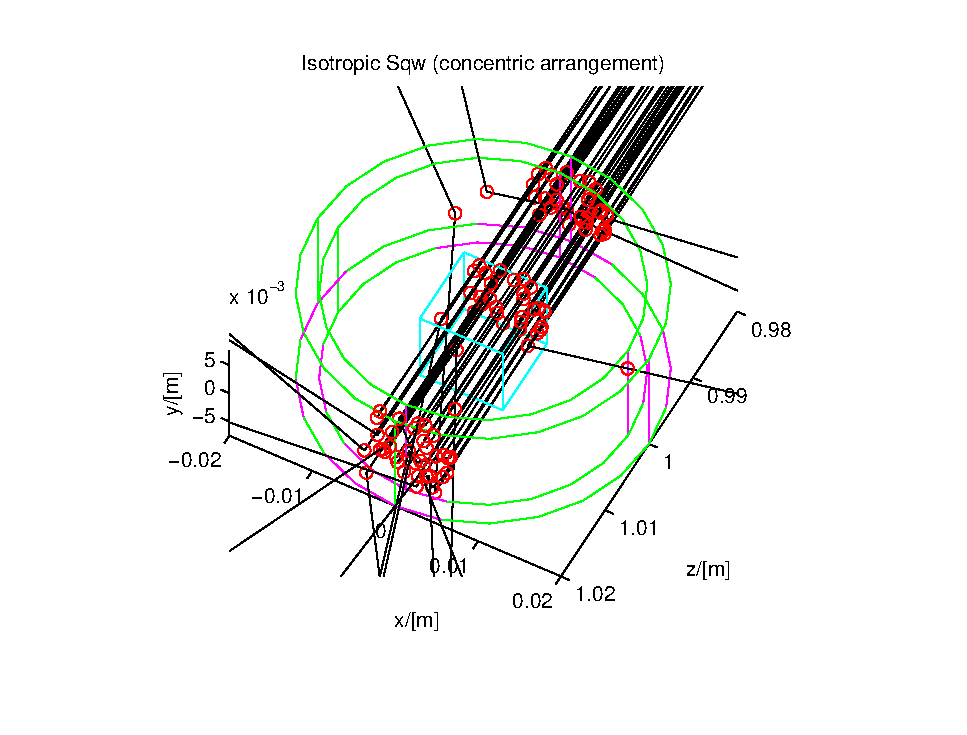
\includegraphics[width=0.9\textwidth]{figures/sqw.eps}
  \end{center}
\caption{An $l-^4$He sample in a cryostat, simulated with the Isotropic\_Sqw component in concentric geometry.}
\label{f:isotropic-sqw}
\end{figure}

The sample component \emph{Isotropic\_Sqw} has been developed in order to simulate neutron scattering from any isotropic material such as liquids, glasses (amorphous systems), polymers and powders (currently, mono-crystals cannot be handled).
The component treats coherent and incoherent neutron scattering and may be used to model most materials, including sample environments with concentric geometries.
The structure and dynamics of isotropic samples can be characterised by the dynamic structure factor $S(q,\omega)$, which determines the interaction between neutrons and the sample and therefore can be used as a probability distribution of $\omega$-energy and $q$-momentum transfers. It handles coherent and incoherent processes, both for elastic and inelastic interactions.
The main input for the component is $S(q,\omega)$ tables, or powder structure files.

Usage examples of this component can be found in the \\
\verb+Neutron site/tests/Test_Isotropic_Sqw+, the \\
\verb+Neutron site/ILL/ILL_H15_IN6+ and the \verb+ILL_TOF_Env+ instruments from the \verb+mcgui+.

\subsection{Neutron interaction with matter - overview}

When a neutron enters a material, according to usual models, it 'sees' atoms as disks with a surface equal to the total cross section of the material $\sigma_{tot}$. The latter includes absorption, coherent and incoherent contributions, which all depend on the incoming neutron energy.
The transmission probability follows an exponential decay law accounting for the total cross section.

For the neutron which is not transmitted, we select a scattering position along the path, taking into account the secondary extinction and absorption probability. In this process, the neutron is considered to be a particle or an attenuated wave.

Once a scattering position has been assigned, the neutron interacts with a material excitation. Here we turn to the wave description of the neutron, which interacts with the whole sample volume. The distribution of excitations, which determines their relative intensity in the scattered beam, is simply the dynamic structure factor - or scattering law - $S(q,\omega)$. We shall build probability distributions from the scattering law in order to improve the efficiency of the method by favoring the $(q,\omega)$ choice towards high $S(q,\omega)$ regions.

The neutron leaves the scattering point when a suitable $(q, \omega)$ choice has been found to satisfy the conservation laws. The method is iterated until the neutron leaves the volume of the material, therefore allowing multiple scattering contributions, which will be considered in more details below.

No experimental method makes it possible to accurately measure the multiple scattering contribution, even though it can become significant at low $q$ transfers (below the first diffraction maximum), where the single scattering coherent signal is weak in most materials. This is why attemps have been made to reduce the multiple scattering contribution by partitioning the sample with absorbing layers. However, this is not always applicable thus makiong the simulation approach very valuable.

The method presented here for handling neutron interaction with isotropic materials is similar in many respects to the earlier MSC \cite{msc}, Discus \cite{discus} and MSCAT \cite{mscat} methods, but the implementation presented here is part of a more general treatment of a sample in an instrument.

\subsection{Theoretical side}

\subsubsection{Pair correlation function $g(r)$ and Dynamic structure factor $S(q,\omega)$}

In the following, we consider an isotropic medium irradiated with a cold or thermal neutron beam. We ignore the possible thermal fission events and assume that the incoming neutron energy does not correspond to a Breit-Wigner resonance in the material. Furthermore, we do not take into account quantum effects in the material, nor refraction and primary extinction.

Following Squires \cite{squires}, the experimental counterpart of the scattering law $S(q,\omega)$ is the neutron double differential scattering cross section for both coherent and incoherent processes:
\begin{equation}\label{eq:d2sigma}
\frac{d^2\sigma}{d\Omega dE_f} = \frac{\sigma}{4\pi}\frac{k_f}{k_i} N S(q, \omega)
\end{equation}
which describes the amount of neutrons scattered per unit solid angle $d\Omega$ and per unit final energy $dE_f$. In this equation, $N=\rho V$ is the number of atoms in the scattering volume $V$ with atomic number density $\rho$, $E_f, E_i, k_f, k_i$ are the kinetic energy and wavevectors of final and initial states respectively, $\sigma$ is the bound atom scattering cross-section, $\Omega$ is the solid angle and $q,\omega$ are the wave-vector and energy transfer at the sample. In practice, the double differential cross section is a linear combinaison of the coherent and incoherent parts as:
\begin{equation}
\label{eq:S=coh+inc}
\sigma S(q,\omega) = \sigma_{coh} S_{coh}(q,\omega) + \sigma_{inc} S_{inc}(q,\omega)
\end{equation}
where the subscripts $coh$ and $inc$ stand for the coherent and incoherent contributions respectively.

We define its norm on a selected $q$ range:
\begin{equation}
|S| = \iint S(q,\omega) dq d\omega .
\end{equation}
The norm $\lim_{q \rightarrow \infty} |S| \simeq q$ for large $q$ values, and can only be defined on a restricted $q$ range.

Some easily measureable coherent quantities in a liquid are the \emph{static pair correlation function} $g(r)$ and the \emph{structure factor} $S(q)$, defined as:
\begin{eqnarray}
\rho g(\vec{r}) &=& \frac{1}{N} \sum_{i=1}^N \sum_{j \neq i} \langle \delta(\vec{r}+\vec{r}_i-\vec{r}_j) \rangle \\
S(\vec{q}) &=&\int S(\vec q,\omega) d\omega \label{eq:sq} \\
           &=&1 + \rho \int_V [g(\vec{r})-1] e^{i\vec{q}.\vec{r}} d\vec{r} \\
           &=&1 + \rho \int_{0}^{\infty} [g(r)-1] \frac{\sin(qr)}{qr} 4 \pi r^2 dr {\rm\ in\ isotropic\ materials.}
\end{eqnarray}
The latter expression, in isotropic materials, may be Fourier transformed as:
\begin{equation}
\label{eq:gr-sq}
g(r)-1 =\frac{1}{2\pi^2 \rho} \int_0^\infty q^2 [S(q) -1] \frac{sin(qr)}{qr} dq
\end{equation}
Both $g(r)$ and $S(q)$ converge to unity for large $r$ and $q$ values respectively, and they are representative of the atoms spatial distribution. In a liquid $\lim_{q \rightarrow 0} S(q) = \rho k_B T \chi_T$ where $\chi_T=(\frac{\partial \rho}{\partial P})_{V,T}$ is the compressibility \cite{Egelstaff67,fischer05}. In perfect gases, $S(q) = 1$ for all $q$. These quantities are obtained experimentally from diffractometers.
In principle, $S_{inc}(q) = 1$ in all materials, but a $q$ dependence is rather usual, partly due to the Debye-Waller factor $e^{-q^2 \langle u^2 \rangle}$. Anyway, $S_{inc}(q)$ converges to unity at high $q$.

The static pair correlation function $g(r)$ is the probability to find a neighbouring atom at a given distance (unitless). Since $g(0) = 0$, Eq. (\ref{eq:gr-sq}) provides a useful normalisation sum-rule for coherent $S(q)$:
\begin{equation}
\label{eq:sq-nomr1}
\int_0^\infty q^2 [S(q) - 1] dq = -2\pi^2\rho {\rm\ for\ coherent\ contribution.}
\end{equation}
This means that the integrated oscillations (around 1) of $S_{coh}(q)$ are directly related to the density of the material $\rho$.
In practice, the function $S(q)$ is often known on a restricted range $q \in [0, q_{max} ]$, due to either limitations in the sample molecular dynamics simulation, or the measurement itself.
In first approximation we consider that Eq. (\ref{eq:sq-nomr1}) can be applied in this range, i.e. we neglect the large $q$ contributions provided $S(q)-1$ converges faster than $1/q^2$. This is usually true after 2-3 oscillations of $S(q)$ in liquids.
Then, in isotropic liquid-like materials, Eq. (\ref{eq:sq-nomr1}) provides a normalisation sum-rule for $S$.

\subsection{Theoretical side - scattering in the sample}

The Eq. \ref{eq:d2sigma} controls the scattering in the whole sample volume.
Its implementation in a propagative Monte Carlo neutron code such as \emph{McStas} can be summarised as follows:
\begin{enumerate}
{\item Compute the propagation path length in the material by geometrical intersections between the neutron trajectory and the sample volume.}
{\item Evaluate the total cross section from the integration of the scattering law over the accessible dynamical range (Section \ref{s:inter-proba}).}
{\item Use the total cross section to determine the probability of interaction for each neutron along the path length, and select a scattering position.}
{\item Weight neutron interaction with the absorption probability and select the type of interaction (coherent or incoherent).}
{\item Select the wave vector and energy transfer from the dynamic structure factor $S(q,\omega)$ used as a probability distribution (Section \ref{s:choose-qw}). Apply the detailed balance.}
{\item Check whether selection rules can be solved (Section \ref{s:rules-qw}). If they cannot, repeat (5).}
\end{enumerate}
This procedure is iterated until the neutron leaves the sample. We shall now detail the key steps of this implementation.

\subsubsection{Evaluating the cross sections and interaction probability}
\label{s:inter-proba}

Following Sears \cite{Sears75}, the total scattering cross section for incoming neutrons with initial energy $E_i$ is
\begin{equation}
\label{eq:iisigma}
\sigma_s(E_i) = \iint \frac{d^2 \sigma}{d\Omega dE_f} d\Omega dE_f = \frac{N \sigma}{4\pi} \iint \frac{k_f}{k_i} S(q, \omega) d\Omega dE_f
\end{equation}
where the integration runs over the entire space and all final neutron energies.
As the dynamic structure factor is defined in the $q,\omega$ space, the integration requires a variable change. Using the momentum conservation law and the solid angle relation $\Omega=2\pi(1-cos \theta)$, were $\theta$ is the solid angle opening, we draw:
\begin{equation}
\label{eq:iqSqw}
\sigma_s(E_i) = N \iint \frac{\sigma S(q,\omega) q}{2 k_i^2} dq d\omega.
\end{equation}
This integration runs over the whole accessible $q,\omega$ dynamical range for each incoming neutron.
In practice, the knowledge of the dynamic structure factor is defined over a limited area with $q \in [q_{min}, q_{max}]$ and $\omega \in [\omega_{min}, \omega_{max}]$ which is constrained by the method for obtaining $S(q,\omega)$, i.e. from previous experiments, molecular dynamics simulations, and analytical models. It is desirable that this area be as large as possible, starting from 0 for both ranges. If we use $\omega_{min} \rightarrow 0$, $q_{min} \rightarrow 0$, $\omega_{max} > 4E_i$ and $q_{max} > 2k_i$, we completely describe all scattering processes for incoming neutrons with wavevector $k_i$ \cite{msc}.

This means that in order to correctly estimate the total intensity and multiple scattering, the knowledge of $S(q,\omega)$ must be wider (at least twice in $q$, as stated previously) than the measurable range in the corresponding experiment.
As a side effect, a self consistent iterative method for finding the true scattering law from the measurement itself is not theorically feasible, except for providing crude approximations.
However, that measured dynamic structure factor may be used to estimate the multiple scattering for a further measurement using longer wavelength neutrons.
In that case, extrapolating the scattering law beyond the accessible measurement ranges might improve substantially the accuracy of the method, but this discussion is beyond the scope of this paper.

Consequently, limiting the $q$ integration in Eq. \ref{eq:iqSqw} to the maximum momentum transfer for elastic processes $2 k_i$, we write the total scattering cross section as
\begin{equation}
\label{eq:iqSq}
\sigma_s(E_i) \simeq \frac{N}{2 k_i^2} \int_0^{2k_i} q \sigma S(q) dq.
\end{equation}
Using Eq. \ref{eq:S=coh+inc}, it is possible to define similar expressions for the coherent and incoherent terms $\sigma_{coh}(E_i)$ and $\sigma_{inc}(E_i)$ respectively. These integrated cross sections are usually quite different from the tabulated values \cite{ILLblue} since the latter are bound scattering cross sections.

Except for a few materials with absorption resonances in the cold-thermal energy range, the absorption cross section for an incoming neutron of velocity $v_i=\sqrt{2E_i/m}$, where $m$ is the neutron mass, is computed as
$\sigma_{abs}(E_i) = \sigma_{abs}^{{\rm 2200}}\frac{2200 m/s}{\sqrt{2E_i/m}}$, where $\sigma_{abs}^{{\rm 2200}}$ is obtained from the literature \cite{ILLblue}.

We now determine the total cross section accounting for both scattering and absorption
\begin{equation}
\sigma_{tot}(E_i) = \sigma_{abs}(E_i) + \sigma_s(Ei).
\end{equation}
The neutron trajectory intersection with the sample geometry provides the total path length in the sample $d_{exit}$ to the exit.
Defining the linear attenuation $\mu(E_i) = \rho\sigma_{tot}(E_i)$, the probability that the neutron event is transmitted along path $d_{exit}$ is $e^{-\mu(E_i) d_{exit}}$.

If the neutron event is transmitted, it leaves the sample. In previous Monte Carlo codes such as DISCUSS \cite{discus}, MSC \cite{msc} and MSCAT \cite{mscat}, each neutron event is forced to scatter to the detector area in order to improve the sample scattering simulation statistics and reduce the computing time. The corresponding instrument model is limited to a neutron event source, a sample and a detector. It is equaly possible in the current implementation to 'force' neutron events to scatter by applying a correction factor $\pi_0=1-e^{-\mu(E_i) d_{exit}}$ to the neutron statistical weight. However, the \emph{McStas} instrument model is often build from a large sequence of components. Eventhough the instrument description starts as well with a neutron event source, more than one sample may be encountered in the course of the neutron propagation and multiple detectors may be positioned anywhere in space, as well as other instrument components (e.g. neutron optics). This implies that neutron events scattered from a sample volume should not focus to a single area.  Indeed, transmitted events may reach other scattering materials and it is not desirable to force all neutron events to scatter. The correction factor $\pi_0$ is then not applied, and neutron events can be transmitted through the sample volume. The simulation efficiency for the scattering then drops significantly, but enables to model much more complex arrangements such as concentric sample environments, magnets and monochromator mechanical parts, and neutron filters.

If the neutron is not transmitted, the neutron statistical weight is multiplied by a factor
\begin{equation}
\pi_1 = \frac{\sigma_s(E_i)}{\sigma_{tot}(E_i)}
\end{equation}
to account for the fraction of absorbed neutrons along the path, and we may in the following treat the event as a scattering event.
Additionally, the type of interaction (coherent or incoherent) is chosen randomly with fractions $\sigma_{coh}(E_i)$ and $\sigma_{inc}(E_i)$.

The position of the neutron scattering event along the neutron trajectory length $d_{exit}$ is determined by \cite{Mildner77,discus}
\begin{equation}
d_{s} = -\frac{1}{\mu(E_i)} \ln(1 - \xi[1 -e^{-\mu(E_i) d_{exit}}])
\end{equation}
where $\xi$ is a random number in [0,1]. This expression takes into account secondary extinction, originating from the decrease of the beam intensity through the sample (self shielding).

\subsubsection{Choosing the $q$ and $\omega$ transfer from $S(q, \omega)$ }
\label{s:choose-qw}

The choice of the $(q, \omega)$ wavevector-energy transfer pair could be done randomly, as in the first event of the second order scattering evaluation in DISCUS \cite{discus}, but it is somewhat inefficient except for materials showing a broad quasi-elastic signal. As the scattering originates from structural peaks and excitations in the material $S(q, \omega)$, it is usual \cite{mscat} to adopt an importance sampling scheme by focusing the $(q, \omega)$ choice to areas where the intensity of $S(q, \omega)$ is high. In practice, this means that the neutron event should scatter preferably on e.g. Bragg peaks, quasielastic contribution and phonons.

The main idea to implement the scattering from $S(q, \omega)$ is to cast two consecutive Monte Carlo choices, using probability distribution built from the dynamic structure factor.
We define first the probability $P_{\omega}(\omega)$ as the \emph{unweighted} fraction of modes whose energy lies between $\omega$ and $\omega+d\omega$
\begin{equation}
P_{\omega}(\omega) d\omega = \frac{\int_0^{q_{max}} q S(q,\omega) dq}{|S|},
\end{equation}
where $|S| = \iint S(q,\omega) dq d\omega$ is the norm of $S(q,\omega)$ in the available dynamical range $q \in [q_{min}, q_{max}]$ and $\omega \in [\omega_{min}, \omega_{max}]$.
The probability $P_{\omega}(\omega)$ is normalised to unity, $\int P_{\omega}(\omega) d\omega = 1$, and is a probability distribution of mode energies in the material. We then choose randomly an energy transfer $\omega$ from this distribution.

Similarly, in order to focus the wavevector transfer choice, we define the probability distribution of wavevector $P_q(q\mid\omega)$ for the selected energy transfer lying between $\omega$ and $\omega+d\omega$
\begin{equation}
P_q(q\mid\omega) = \frac{q S(q, \omega)}{S(q)},
\end{equation}
from which we choose randomly a wavevector transfer $q$, knowing the energy transfer $\omega$.
These two probability distributions extracted from $S(q,\omega)$ are shown in Fig. \ref{f:isotropic-sqw-proba}, for a model $S(q,\omega)$ function built from the {\it l}-$^4$He elementary excitation (Data from Donnelly).

\begin{figure}
  \begin{center}
    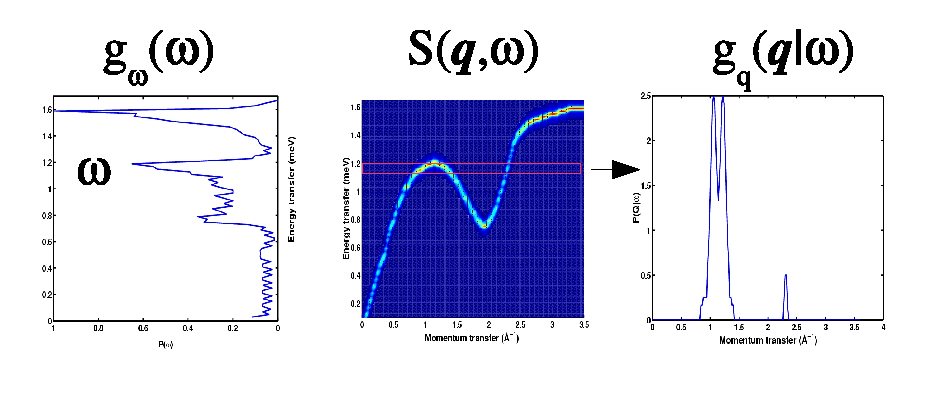
\includegraphics[width=0.9\textwidth]{figures/Sqw_sampling.eps}
  \end{center}
\caption{\emph{Centre}: Model of dynamic structure factor $S(q,\omega)$ for l-$^4$He ; \emph{left}: probability distribution $g_\omega$ (horizontal axis) of energy transfers (vertical axis, density of states) ; \emph{right} : probability distribution $g_q(\omega)$ (vertical axis) of momentum transfers (horizontal axis) for a given energy transfer $\hbar \omega \sim 1.1$ meV.}
\label{f:isotropic-sqw-proba}
\end{figure}

Then a selection between energy gain and loss is performed with the detailed balance ratio $e^{-\hbar \omega / k_B T}$. In the case of Stokes processes, the neutron can not loose more than its own energy to the sample dynamics, so that $\hbar \omega < E_i$. This condition breaks the symmetry between up-scattering and down-scattering.

\subsubsection{Solving selection rules and choosing the scattered wave vector}
\label{s:rules-qw}

The next step is to check that the conservation laws
\begin{eqnarray}
\hbar \omega &=& E_i - E_f = \frac{\hbar^2}{2m}(k_i^2 - k_f^2) \label{eq:sqw-w-transfer} \\
\vec q &=& \vec k_i - \vec k_f \label{eq:sqw-q-transfer}
\end{eqnarray}
can be satisfied. These conditions are closely related to the method for selecting the outgoing wave vector direction.

When the final wave vector has to be computed, the quantities $\vec{k}_i$, $\hbar \omega$ and $q = |\vec{q}|$ are known.
We solve the energy conservation law Eq. (\ref{eq:sqw-w-transfer}) and we select randomly $k_f$ as one of the two roots.

The scattering angle $\theta$ from the initial $k_i$ direction is determined from the momentum conservation law $cos(\theta) = (k_i^2 + k_f^2 - q^2)/(2k_i k_f)$, which defines a scattering cone. We then choose randomly a direction on the cone.

If the selection rules can not be verified (namely $|cos(\theta)| > 1$), a new $(q,\omega)$ random choice is performed (see Section \ref{s:choose-qw}).
It might appear inefficient to select the energy and momentum tranfers first and check the selection rules afterwards. However, in practice, the number of iterations to actually scatter on a high probability process and satisfy these rules is limited, usually below 10. Moreover, as these two steps are simple, the whole process requires a limited number of computer operations.

As mentioned in Section \ref{s:inter-proba}, previous multiple scattering estimation codes \cite{msc,mscat,discus} force the outgoing neutron event to come into the detector area and time window, thus improving dramatically the code efficiency. This choice sets the measurable energy and momentum transfers for the last scattering event in the sample, so that the choice of the scattering excitation actually requires a more complex sampling mechanism for the dynamic structure factor. As the present implementation makes no assumption on the simulated instrument part which is behind the sample, we can not apply this method. Consequently, the efficiency of the sample scattering code is certainly lower than previous codes, but on the other hand it does not depend on the type of instrument simulation. In particular, it may be used to model any material in the course of the neutron propagation along the instrument model (filters, mechanical parts, samples, shields, radiation protections).

Once the scattering probability and position, the energy and momentum transfers and the neutron momentum after scattering have all been defined, the whole process is iterated until the neutron is transmitted and exits the sample volume.

\subsubsection{Extension to powder elastic scattering}

In principle, the component can work in purely elastic mode if only the $\omega = 0$ column is available in $S$.
Anyway, in the diffractionists world, people do not usually define scattering with $S(q)$ (Eq. \ref{eq:sq}), but through the scattering vector $\boldsymbol{\tau}$, multiplicity $z(\tau)$ (for powders), and $|F^2|$ structure factors including Debye-Waller factors, as in Eq. \ref{eq:sigma_coh_el}.

When doing diffraction, and neglecting inelastic contribution as first approximation, we may integrate Eq. \ref{eq:d2sigma}, keeping $k_i = k_f$.
\begin{eqnarray}
\left(\frac{d\sigma}{d\Omega}\right)_{\rm coh.el.}(|q|) &=& \int_0^\infty \frac{d^2\sigma_{coh}}{d\Omega dE_f} dE_f = \frac{N \sigma_{coh}}{4\pi} S_{coh}(q) \\
& = & N\frac{(2\pi)^3}{V_0}\sum_{\boldsymbol{\tau}} \delta(\boldsymbol{\tau} - \boldsymbol{q})|F_{\boldsymbol{\tau}}|^2 {\rm\ from\ Eq.\ (\ref{eq:sigma_coh_el})}
\end{eqnarray}
with $V_0 = 1/\rho$ being the volume of a lattice unit cell. Then we come to the formal equivalence, in the powder case \cite{squires} (integration over Debye-Scherrer cones):
\begin{eqnarray}\label{eq:sq-F2}
S_{coh}(q) = \frac{\pi \rho}{2\sigma_{coh}} \frac{z(q)}{q^2} |F_q|^2 {\rm\ in\ a\ powder.}
\end{eqnarray}
for each lattice Bragg peak wave vector $q$.
The normalisation rule Eq. (\ref{eq:sq-nomr1}) can not usually be applied for powders, as the $S(q)$ is a set of Dirac peaks for which the $\int q^2 S(q) dq$ is difficult to compute, and $S(q)$ does not converge to unity for large $q$. Each $F^2$ Dirac contribution may be broaden when specifiying a diffraction peak width.

Of course, the component PowderN (see section \ref{powder}) can handle powder samples efficiently (faster, better accuracy), but does not take into account multiple scattering, nor secondary extinction (which is significant for materials with large absorption cross sections). On the other side, the current Isotropic\_Sqw component assumes a powder packing factor of 1 (massive sample). To change into a lower packing factor, use a lower powder density.

\subsubsection{Important remarks and limitations}

Since the choice of the interaction type, we know that the neutron \emph{must} scatter, with an appropriate $\vec k_f$ outgoing wave vector. If any of the choices in the method fails:
\begin{enumerate}
\item the two roots $k_f^+$ and $k_f^-$ are imaginary, which means that conservation laws can not be satisfied and for instance the selected energy transfer is higher than the incoming neutron energy
\item the radius of the target circle is imaginary, that is $|cos(\theta)| > 1$.
\end{enumerate}
then a new $(q, \omega)$ set is drawn, and the process is iterated until success or - at last - removal of the neutron event. These latter absorptions are then reported at the end of the simulation, as it never occurs in reality - neutrons that scatter do find a suitable $(q, \omega)$ set.\index{Removed neutron events}

The $S(q,\omega)$ data sets should be as wide a possible in $q$ and $\omega$ range, else scattering conditions will be limited by the reduced data set (specially multiple scattering estimates). On the other hand, when $q$ and $\omega$ ranges are too large, some Monte Carlo choices lead to scattering temptatives in non useful regions of $S$, which reduces dramatically the algorithm efficiency.

The best settings are:
\begin{enumerate}
\item to have the widest $q$ and $\omega$ range for $S(q,\omega)$ data sets,
\item to either set $wmax$ and $qmax$ to the maximum scatterable energy and wavevectors,
\item or alternatively request the automatic range optimisation by setting parameter \verb+auto_qw=1+. This is recommended, but may sometimes miss a few neutrons if the $q,\omega$ beam range has been guessed too small.
\end{enumerate}

Focusing the $q$ and $\omega$ range (e.g. with 'auto\_qw=1'), to the one being able to scatter the incoming beam, when using the component does improve significantly the speed of the computation. Additionally, if you restrict the scattering to the first order only (parameter 'order=1'), then you may specify the angular vertical extension $d\phi$ of the scattering area to gain optimised focusing. This option does not apply when handling multiple scattering (which emits in $4\pi$ many times before exiting the sample).

A bilinear interpolation for the $q,\omega$ determination is used to improve the accuracy on the scattered intensity, but it may be unactivated when setting parameter \verb+interpolate=0+. This will often result in a discrete $q,\omega$ sampling.

As indicated in the previous section, the Isotropic\_Sqw component is not as efficient as PowderN for powder single scattering, but handles scattering processes in a more accurate way (secondary extinction, multiple scattering).

\subsection{The implementation}

\begin{table}
  \begin{center}
  {\let\my=\\
    \begin{tabular}{|lr|p{0.6\textwidth}|}
    \hline
Parameter & type & meaning \\
    \hline
Sqw\_coh   & string              & Coherent scattering data file name. Use 0, NULL or "" to disable  \\
Sqw\_inc   & string              & Incoherent scattering data file name. Use 0, NULL or "" to scatter isotropically (Vanadium like)  \\
sigma\_coh & [barns]      & Coherent scattering cross-section. -1 to disable \\
sigma\_inc & [barns]      & Incoherent scattering cross-section. -1 to disable \\
sigma\_abs & [barns]      & Absorption cross-section. -1 to disable  \\
V\_rho     & [\AA$^{-3}$] & atomic number density. May also be specified with molar weight \emph{weight} in [g/mol] and material \emph{density} in [g/cm$^3$] \\
T          & [K]          & Temperature. 0 disables detailed balance \\
    \hline
xwidth   & [m] & \\
yheight  & [m] & dimensions of a box shaped geometry \\
zdepth   & [m] & \\
radius\_o & [m] & dimensions of a cylinder shaped geometry  \\
radius\_i & [m] & sphere geometry if radius\_i=0  \\
thickness& [m] & thickness of hollow shape  \\
    \hline
auto\_qw  & boolean & Automatically optimise probability tables during simulation  \\
auto\_norm& scalar  & Normalize $S(q,\omega)$ when -1, use raw data when 0, multiply $S$ by given value when positive \\
%interpolate & boolean & Smooth $S(q,\omega)$ table (recommended) \\
order     & integer & Limit multiple scattering up to given order. 0 means all orders  \\
concentric& boolean & Enables to 'enter' inside concentric hollow geometries  \\
    \hline
    \end{tabular}
    \caption{Main Isotropic\_Sqw component parameters}
    \label{t:sqw-param}
  }
  \end{center}
\end{table}

\subsubsection{Geometry}

The geometry for the component may be box, cylinder and sphere shaped, either filled or hollow. Relevant parameters for this purpose are as follow:
\begin{itemize}
\item {\bf box}: dimensions are $x_{width} \times y_{height} \times z_{depth}$.
\item {\bf box, hollow}: \emph{idem}, and the side wall thickness is set with $thickness$.
\item {\bf cylinder}: dimensions are $r$ for the radius and $y_{height}$ for the height.
\item {\bf cylinder, hollow}: \emph{idem}, and hollow part is set with $thickness$.
\item {\bf sphere}: dimension is $r$ for the radius.
\item {\bf sphere, hollow}: \emph{idem}, and hollow part is set with $thickness$.
\end{itemize}
The AT position corresponds to the centre of the sample.

Hollow shapes are particularly useful to model complex sample environments. Refer to the dedicated section below for more details on this topic.

\subsubsection{Dynamical structure factor}

The material behaviour is specified through the total scattering cross-sections $\sigma_{coh}$, $\sigma_{inc}$, $\sigma_{abs}$, and the $S(q, \omega)$ data files.

If you are lucky enough to have access to separated coherent and incoherent contributions (e.g. from material simulation), simply set Sqw\_coh and Sqw\_inc parameter to the files names. If on the other hand you have access to a global data set containing incoherent scattering as well (e.g. the result of a previous experiment), use Sqw\_coh parameter, set the $\sigma_{coh}$ parameter to the sum of both contributions $\sigma_{coh}+\sigma_{inc}$, and set $\sigma_{inc}=-1$. This way we only use one of the two implemented  scattering channels. Such global data sets may originate from previous experiments, as far as you have applied all known corrections (multiple scattering, geometry, ...).

In any case, the accuracy of the $S(q, \omega)$ data limits the $q$ and $\omega$ resolution of the simulation, eventhough a bilinear interpolation is performed in order to smooth binning. The sampling of data files should then be as thin as possible.

If the Sqw\_inc parameter is left unset but the $\sigma_{inc}$ is \emph{not} zero, an isotropic incoherent elastic scattering is used, just like the V\_sample component (see section \ref{s:v_sample}).

Anyway, as explained below, it is also possible to simulate the elastic scattering from a powder file (see below).

\subsubsection{File formats: $S(q,\omega)$ inelastic scattering}

The format of the data files is free text, consisting of three numerical blocks, separated by empty lines or comments, in the following order
\begin{enumerate}
\item A vector of length $m$ containing wavevector $q$ values, in \AA$^{-1}$.
\item A vector of length $n$ containing energy $\omega$ values, in meV.
\item A matrix of size $m$ rows by $n$ columns, of $S(q, \omega)$ values, in meV$^{-1}$.
\end{enumerate}
Any line beginning with any character of \verb+#;/%+ is considered to be a comment, and lines which can not be read as vectors/matrices are ignored.

The file header may optionally contain parameter settings for the material, as comments, with keywords as in the following example:
\begin{verbatim}
  #V_0         35   cell volume [Angs^3]
  #V_rho       0.07 atom number density [at/Angs^3]
  #sigma_abs   5    absorption cross section [barns]
  #sigma_inc   4.8  incoherent cross section [barns]
  #sigma_coh   1    coherent cross section  [barns]
  #Temperature 10   for detailed balance [K]
  #density     1    material density [g/cm^3]
  #weight      18   material molar weight [g/mol]
  #nb_atoms    6    number of atoms per unit cell
\end{verbatim}
Some \verb+sqw+ data files are included in the \MCS\ distribution data directory, and they contain material parameter settings in their header, so that you may use:
\begin{verbatim}
Isotropic_Sqw(<geometry parameters>, Sqw_coh="He4_liq_coh.sqw", T=4)
\end{verbatim}

Example files are listed as \verb+*.sqw+ files in directory \verb+MCSTAS/data+. A table of $S(q,\omega)$ data files for a few liquids are listed in Table \ref{t:liquids-data} (page \pageref{t:liquids-data}).

\subsubsection{File formats: $S(q)$ liquids}

This file format provides a mean to import directly an $S(q)$ data set, when setting parameters:
\begin{verbatim}
  powder_format=qSq
\end{verbatim}
The 'Sqw\_coh' (or 'Sqw\_inc') file should contains a single numerical block, which column assignment is defaulted as $q$ and $S(q)$ being the first and second column respectively. This may be overridden from the file header with '\#column' keywords, as in the example:
\begin{verbatim}
  #column_q  2
  #column_Sq 1
\end{verbatim}
Such files can only handle elastic scattering.

\subsubsection{File formats: powder structures (LAZY, Fullprof, Crystallographica)}

Data files as used by the component PowderN may also be read. Data files of type \verb'lau' and \verb'laz' in the \MCS\ distribution data directory are self-documented in their header. They do not need any additional parameters to be used, as in the example:
\begin{verbatim}
  Isotropic_Sqw(<geometry parameters>, Sqw_coh="Al.laz")
\end{verbatim}
Other column-based file formats may also be imported e.g. with parameters such as:
\begin{verbatim}
  powder_format=Crystallographica
  powder_format=Fullprof
  powder_Dd    =0
  powder_DW    =1
\end{verbatim}
The last two parameters may as well be specified in the data file header with lines:
\begin{verbatim}
  #Debye_Waller 1
  #Delta_d/d    1e-3
\end{verbatim}
The powder description is then translated into $S(q)$ by using Eq. (\ref{eq:sq-F2}).
In this case, the density $\rho = n/V_0$ is the number of atoms in the inverse volume of the unit cell.

As the component builds an $S(q)$ from the powder structure description, the accuracy of the Isotropic\_Sqw component is limited by the binning during that conversion. This is usually enough to describe sample environments including powders (aluminium, copper, ...), but it is recommended to rather use PowderN for faster and accurate powder diffraction, eventthough this latter does not implement multiple scattering.

Such files can only handle elastic scattering. A list of common powder definition files is available in Table \ref{t:powders-data} (page \pageref{t:powders-data}).

\subsubsection{Concentric geometries, sample environment}
\index{Sample environments}

The component has been designed in a way which enables to describe complex imbricated set-ups, i.e. what you need to simulate sample environments. To do so, one has first to use hollow shapes, then keep in mind that each surrounding geometry should be first declared before the central position (usually the sample) with the \verb+concentric=1+ parameter, but also duplicated (with an other instance name) at a symmetric position with regards to the centre as in the example (shown in Fig. \ref{f:isotropic-sqw}):
\begin{verbatim}
COMPONENT s_in=Isotropic_Sqw(
  thickness=0.001, radius=0.02, yheight=0.015,
  Sqw_coh="Al.laz", concentric=1)
AT (0,0,1) RELATIVE a

COMPONENT sample=Isotropic_Sqw(
  xwidth=0.01, yheight=0.01, zdepth=0.01,
  Sqw_coh="Rb_liq_coh.sqw")
AT (0,0,1) RELATIVE a

COMPONENT s_out=Isotropic_Sqw(
  thickness=0.001, radius=0.02, yheight=0.015,
  Sqw_coh="Al.laz")
AT (0,0,1) RELATIVE a
\end{verbatim}
Central component may be of any type, not specifically an Isotropic\_Sqw instance. It could be for instance a Single\_crystal or a PowderN.
In principle, the number of surrounding shells is not restricted.
The only restriction is that neutrons that scatter (in $4\pi$) can not come back in the instrument description, so that some of the multiple scattering events are lost. Namely, in the previous example, neutrons scattered by the outer wall of the cryostat \verb+s_out+ can not come back to the sample or to the other cryostat wall \verb+s_in+. As these neutrons have usually few chances to reach the rest of the simulation, we expect that the approximation is fair.

\subsection{Validation}
For constant incoherent scattering mode, V\_sample, PowderN, Single\_crystal and Isotropic\_Sqw produce equivalent results, eventhough the two later are more accurate (geometry, multiple scattering). Execution times are equivalent.

Compared with the PowderN component, the $S(q)$ method is twice slower in computation time, and intensity is usually lower by typically 20 \% (depending on scattering cross sections), the difference arising from multiple scattering and secondary extinction (not handled in PowderN). The PowderN component is intrinsically more accurate in $q$ as each Bragg peak is handled separately as an exact Dirac peak, with optional $\Delta q$ spreading. In Isotropic\_Sqw, an approximated $S(q)$ table is built from the $F^2$ data, and is coarser. Still, differences in the diffraction pattern are limited.

The Isotropic\_Sqw component has been benchmarked against real experiment for liquid Rubidium (Copley, 1974) and liquid Cesium (Bodensteiner  and Dorner, 1989), and the agreement is excellent.

The \verb+Test_Isotropic_Sqw+ test/example instrument exists in the distribution for this component.





\chapter{Monitors and detectors}
\index{Library!Components!monitors}
\index{Monitors|textbf}

In real neutron experiments, detectors and monitors play quite
different roles. One wants the detectors to be as efficient as
possible, counting all neutrons (absorbing them in the process),
while the monitors measure the intensity of the incoming beam, and must
as such be almost transparent, interacting only with (roughly) 0.1-1\%
of the neutrons passing by. In computer simulations, it is
of course possible to detect every neutron ray without
absorbing it or disturbing any of its parameters. Hence, the two components
have very similar functions in the simulations, and we do
not distinguish between them. For simplicity, they are from here on
just called {\bf monitors}.

Another important difference between computer simulations
and real experiments is
that one may allow the monitor to be sensitive to any neutron property,
as {\em e.g.} direction, energy, and divergence, in addition to what
is found in real-world detectors (space and time). One may, in
fact, let the monitor record correlations between these properties,
as seen for example in the divergence/position sensitive monitor in
section~\ref{s:divpos-monitor}.

When a monitor detects a neutron ray,
a number counting variable is incremented: $n_i = n_{i-1}+1$.
In addition, the neutron
weight $p_i$ is added to the weight counting variable:
$I_i = I_{i-1} + p_i$,
and the second moment of the weight is
updated: $M_{2,i} = M_{2,i-1} + p_i^2$.
As also discussed chapter \ref{s:MCtechniques}, after a simulation of $N$ rays
the detected intensity (in units of neutrons/sec.) is $I_N$,
while the estimated errorbar is $\sqrt{M_{2,N}^2}$.

Many different monitor components have been developed for
\MCS , but we have decided to support only the most important ones.
One example of the monitors we have omitted is the single monitor,
{\bf Monitor},
that measures just one number (with errorbars) per simulation.
This effect is mirrored by any of the 1- or 2-dimensional components
we support, e.g. the {\rm PSD\_monitor}.
In case additional functionality of monitors is required,
the few code lines of existing monitors can easily be modified.

However, the ultimate solution is the use of the
``Swiss army knife'' of monitors, {\bf Monitor\_nD}, that can face
almost any simulation requirement,
but will prove challenging for users who like to perform own modifications.

\newpage
\section{TOF\_monitor: The time-of-flight monitor}
%\component{TOF\_monitor}{System}{$x_{\rm min}$, $x_{\rm max}$, $y_{\rm min}$, $y_{\rm max}$, $n_{\rm chan}$, $t_0$, $t_1$, filename}{$\Delta t$}{}
\index{Monitors!Time-of-flight monitor}
\mcdoccomp{monitors/TOF_monitor.parms}

The component {\bf TOF\_monitor} has a rectangular opening
in the $(x,y)$ plane, given by the $x$ and $y$ parameters,
like for {\bf Slit}.
The neutron ray is propagated to the plane of the monitor
by the kernel call PROP\_Z0.
A neutron ray is counted if it passes within the rectangular opening
given by the $x$ and $y$ limits.

Special about {\bf TOF\_monitor} is that it is sensitive to
the arrival time, $t$, of the neutron ray.
Like in a real time-of-flight detector, the time dimension is
binned into small time intervals.
Hence this monitor maintains a one-dimensional histogram of counts.
The $n_{\rm chan}$ time intervals begin at $t_0$ and
end at $t_1$ (alternatively, the interval length is specified by $\Delta t$).
As usual in time-of-flight analysis, all times are given in units of $\mu$s.

The output parameters from {\bf TOF\_monitor} are the three count numbers,
$N, I$, and $M_2$ for the total counts in the monitor.
In addition, a file, \verb+filename+, is produced with a list of
the same three data divided in different TOF bins.
This file can be read and plotted by the {\rm mcplot} tool; see the
System Manual.



\section{TOF2E\_monitor: A time-of-flight monitor with simple energy analysis} \label{s:TOF2E_monitor}
\index{Monitors!TOF2E monitor}
%\component{E\_monitor}{System}{$x_{\rm min}$, $x_{\rm max}$, $y_{\rm
%min}$, $y_{\rm max}$, $n_{\rm chan}$, $E_{\rm min}$, $E_{\rm max}$,
%$t_0$, $L_{\rm flight}$, filename}{}{Not validated}
\mcdoccomp{monitors/TOF2E_monitor.parms}

The component {\bf TOF2E\_monitor} resembles {\bf TOF\_monitor}
to a very large extent. Only this monitor converts the neutron flight
time to energy - as would be done in an experiment.
The {\em apparent} neutron energy, $E_{\rm app}$ is calculated 
from the apparent velocity, given by 
\begin{equation}
v_{\rm app} = \frac{L_{\rm flight}}{t-t_0} ,
\end{equation}
where the time offset, $t_0$ defaults to zero.
$E_{\rm app}$ is binned in \textit{nchan} bins between
$E_{\rm min}$ and $E_{\rm max}$ (in meV).

The output parameters from {\bf TOF2E\_monitor} are the total counts,
and a file with 1-dimensional data vs. $E_{\rm app}$, 
similar to {\bf TOF\_monitor}.



\section{E\_monitor: The energy-sensitive monitor} \label{s:E_monitor}
\index{Monitors!Energy monitor}
\component{E\_monitor}{System}{$x_{\rm min}$, $x_{\rm max}$, $y_{\rm min}$, $y_{\rm max}$, $n_{\rm chan}$, $E_{\rm min}$, $E_{\rm max}$, filename}{}{}
The component {\bf E\_monitor} resembles {\bf TOF\_monitor}
to a very large extent. Only this monitor is sensitive to
the neutron energy, which in binned in \textit{nchan} bins between
$E_{\rm min}$ and $E_{\rm max}$ (in meV).

The output parameters from {\bf E\_monitor} are the total counts,
and a file with 1-dimensional data vs. $E$, similar to {\bf TOF\_monitor}.




% Emacs settings: -*-mode: latex; TeX-master: "manual.tex"; -*-


\section{L\_monitor: The wavelength sensitive monitor}
\label{s:L_monitor}
\index{Monitors!Wavelength monitor}

%\component{L\_monitor}{System}{$x_\textrm{min}$, $x_\textrm{max}$, $y_\textrm{min}$, $y_\textrm{max}$, $n_\textrm{chan}$, $\lambda_\textrm{min}$, $\lambda_\textrm{max}$, filename}{}{}
\mcdoccomp{monitors/L_monitor.parms}

The component \textbf{L\_monitor} is very similar to
\textbf{TOF\_monitor} and \textbf{E\_monitor}.
This component is just sensitive to the neutron wavelength.
The wavelength spectrum is output in a one-dimensional histogram.
between $\lambda_\textrm{min}$ and $\lambda_\textrm{max}$ (measured in \AA ).

As for the two other 1-dimensional monitors, this component outputs
the total counts and a file with the histogram.



\section{PSD\_monitor: The PSD monitor}
\index{Monitors!Position sensitive detector (PSD)}
\mcdoccomp{monitors/PSD_monitor.parms}

The component \texttt{PSD\_monitor} resembles other monitors, e.g.
\texttt{Monitor}, and also propagates the photon ray to the detector
surface in the $(x,y)$-plane, where the detector window is set
by the $x$ and $y$ input coordinates.
The PSD monitor is sensitive to the arrival position of the of the photon ray.
The rectangular monitor window, given by the $x$ and $y$
limits is divided into $n_x \times n_y$ pixels.

The output from \texttt{PSD\_monitor} is the integrated counts, $n, I, M_2$,
as well as
three two-dimensional arrays of counts: $n(x,y), I(x,y), M_2(x,y)$.
The arrays are written to a file, \verb+filename+, and can be read e.g. by the tool
\textbf{mxplot}, see the system manual.


% Emacs settings: -*-mode: latex; TeX-master: "manual.tex"; -*-

\section{Divergence\_monitor: A divergence sensitive monitor}
\label{s:div-monitor}
\index{Monitors!Divergence monitor}
\component{Divergence\_monitor}{System}{$x_{\rm min}$, $x_{\rm max}$, $y_{\rm min}$, $y_{\rm max}$, $n_{\rm v}$, $n_{\rm h}$, $\eta_{\rm v,max}$, $\eta_{\rm h,max}$, filename}{}{}


The component {\bf Divergence\_monitor} is a two-dimensional monitor,
which resembles {\bf PSD\_Monitor}. As for this component,
the detector window is set
by the $x$ and $y$ input coordinates.
{\bf Divergence\_ monitor} is sensitive to the neutron divergence,
defined by
$\eta_{\rm h} = \tan^{-1}(v_x/v_z)$ and $\eta_{\rm v} = \tan^{-1}(v_y/v_z)$.
The neutron counts are being histogrammed
into $n_{\rm v} \times n_{\rm h}$ pixels. 
The divergence range accepted is in the vertical direction
$[-\eta_{\rm v,max}; \eta_{\rm v,max}]$, and similar for the horizontal
direction.

The output from {\bf PSD\_monitor} is the integrated counts, $n, I, M_2$,
as well as
three two-dimensional arrays of counts: $n(\eta_{\rm v},\eta_{\rm h}),
I(\eta_{\rm v},\eta_{\rm h}), M_2(\eta_{\rm v},\eta_{\rm h})$.
The arrays are written to a file, \verb+filename+, 
and can be read e.g. by the tool {\bf MC\_plot}, see the system manual.


\section{DivPos\_monitor: A divergence and position sensitive monitor}
\label{s:divpos-monitor}
\index{Monitors!Divergence/position monitor}
%\component{DivPos\_monitor}{System}{$x_\textrm{min}$, $x_\textrm{max}$, $y_\textrm{min}$, $y_\textrm{max}$, $n_x$, $n_\textrm{h}$, $\eta_\textrm{h,max}$, filename}{}{}
\mcdoccomp{monitors/DivPos_monitor.parms}

\textbf{DivPos\_monitor} is a two-dimensional monitor component,
which is sensitive to both horizontal position ($x$) and horizontal divergence
defined by $\eta_\textrm{h} = \tan^{-1}(v_x/v_z)$.
The detector window is set
by the $x$ and $y$ input coordinates.

The neutron counts are being histogrammed
into $n_x \times n_\textrm{h}$ pixels. The horizontal divergence range accepted is
$[-\eta_\textrm{h,max}; \eta_\textrm{h,max}]$, and the horizontal position
range is the size of the detector.

The output from \textbf{PSD\_monitor} is the integrated counts, $n, I, M_2$,
as well as
three two-dimensional arrays of counts: $n(x,\eta_\textrm{h}),
I(x,\eta_\textrm{h}), M_2(x,\eta_\textrm{h})$.
The arrays are written to a file and can be read e.g. by the tool
\textbf{mcplot}, see the system manual.

This component can be used for measuring acceptance diagrams \cite{Cussen03}.
\textbf{PSD\_monitor} can easily be changed into being sensitive
to $y$ and vertical divergence by a 90 degree rotation around the $z$-axis.


\newpage
\section{Monitor\_nD: A general Monitor for 0D/1D/2D records}
\label{s:monitornd}
\index{Monitors!The All-in-One monitor (Monitor\_nD)}

\component{Monitor\_nD}{System, E. Farhi}{$x_{\rm min}$, $x_{\rm max}$, $y_{\rm min}$, $y_{\rm max}$, options}{$file$, $x_{width}, y_{height}, z_{depth}$, $bins$, $min$, $max$}{}

The component {\bf Monitor\_nD} is a general Monitor that may output any
set of physical parameters regarding the passing neutrons. The
generated files are either a set of 1D signals ([Intensity] {\it vs.}
[Variable]), or a single 2D signal ([Intensity] {\it vs.} [Variable 1]
{\it vs.} [Variable 1]), and possibly a simple long list of selected
physical parameters for each neutron.

The input parameters for {\bf Monitor\_nD} are its dimensions $x_{\rm
  min}, x_{\rm max}, y_{\rm min}$, $y_{\rm max}$ (in meters) and an {\it
  options} string describing what to detect, and what to do with the
signals, in clear language. The $x_{width}, y_{height}, z_{depth}$ may also be used to enter dimensions.

Eventhough the possibilities of Monitor\_nD are numerous, its usage remains as simple as possible, specially in the \verb+options+ parameter, which 'understands' normal language.
The formatting of the {\it options}
parameter is free, as long as it contains some specific keywords, that
can be sometimes followed by values. The {\it no} or {\it not} option
modifier will revert next option. The {\it all} option can also affect a
set of monitor configuration parameters (see below).

As the usage of this component enables to monitor virtually anything, and thus the combinations of options and parameters is infinite, we shall only present the most basic configuration. The reader should refer to the on-line component help, using e.g. \verb+mcdoc Monitor_nD.comp+.

\subsection{The Monitor\_nD geometry}

The monitor shape can be selected among seven geometries:
\begin{enumerate}
\item{({\it square}) The default geometry is flat rectangular in ($xy$)
    plane with dimensions $x_{\rm min}, x_{\rm max}, y_{\rm min}$,
    $y_{\rm max}$, or $x_{width}, y_{height}$.}
\item{({\it box}) A rectangular box with dimensions $x_{width}, y_{height}, z_{depth}$.}
\item{({\it disk}) When choosing this geometry, the detector is a flat
    disk in ($xy$) plane. The radius is then
    \begin{equation}
      \mbox{radius} = \max ( \mbox{abs } [ x_{\rm min}, x_{\rm max}, y_{\rm
        min}, y_{\rm max}, x_{width}/2, y_{height}/2 ] ).
    \end{equation}
    }
\item{({\it sphere}) The detector is a sphere with the same radius as
    for the {\it disk} geometry.}
\item{({\it cylinder}) The detector is a cylinder with revolution axis
    along $y$ (vertical). The radius in ($xz$) plane is
    \begin{equation}
      \mbox{radius} =  \max ( \mbox{abs } [ x_{\rm min}, x_{\rm max}, x_{width}/2 ] ),
    \end{equation}
    and the height along $y$ is
    \begin{equation}
      \mbox{height} =  | y_{\rm max} - y_{\rm max} | {\rm or} y_{height}.
    \end{equation}
    }
\item{({\it banana}) The same as the cylinder, but without the top/bottom caps, and on a restricted angular range. The angular range is specified using a \verb+theta+ variable limit specification in the \verb+options+.}
\item{({\it previous}) The detector has the shape of the previous component. This may be a surface or a volume. In this case, the neutron is detected on previous component, and there is not neutron propagation.}
\end{enumerate}

By default, the monitor is flat, rectangular. Of course, you can choose
the orientation of the {\bf Monitor\_nD} in the instrument description
file with the usual \texttt{ROTATED} modifier.

For the {\it box}, {\it sphere} and {\it cylinder}, the outgoing neutrons are
monitored by default, but you can choose to monitor incoming neutron
with the {\it incoming} option.

At last, the {\it slit} or {\it absorb} option will ask the component to
absorb the neutrons that do not intersect the monitor. The {\it exclusive} option word removes neutrons which are similarly outside the monitor limits (that may be other than geometrical).

The {\it parallel} option keyword is of common use in the case where the {\bf Monitor\_nD} is superposed with other components. It ensures that neutrons are detected independently of other geometrical constrains. This is generally the case when you need e.g. to place more than one monitor at the same place.

\subsection{The neutron parameters that can be monitored}

There are many different variables that can be monitored at the same time
and position. Some can have more than one name (e.g. \texttt{energy} or
\texttt{omega}).


\begin{verbatim}
    kx ky kz k wavevector [Angs-1] (    usually axis are
    vx vy vz v            [m/s]         x=horz., y=vert., z=on axis)
    x y z                 [m]      Distance, Position
    kxy vxy xy radius     [m]      Radial wavevector, velocity and position
    t time                [s]      Time of Flight
    energy omega          [meV]
    lambda wavelength     [Angs]
    p intensity flux      [n/s] or [n/cm^2/s]
    ncounts               [1]
    sx sy sz              [1]      Spin
    vdiv ydiv dy          [deg]    vertical divergence (y)
    hdiv divergence xdiv  [deg]    horizontal divergence (x)
    angle                 [deg]    divergence from  direction
    theta longitude       [deg]    longitude (x/z) [for sphere and cylinder]
    phi   lattitude       [deg]    lattitude (y/z) [for sphere and cylinder]
\end{verbatim}
as well as two other special variables
\begin{verbatim}
    user user1            will monitor the [Mon_Name]_Vars.UserVariable{1|2}
    user2 user3           to be assigned in an other component (see below)
\end{verbatim}

To tell the component what you want to monitor, just add the variable
names in the {\it options} parameter. The data will be sorted into {\it
  bins} cells (default is 20), between some default {\it limits}, that
can also be set by user. The {\it auto} option will automatically
determine what limits should be used to have a good sampling of signals.

\subsection{Important options}

Each monitoring records the flux (sum of weights $p$) versus the
given variables, except if the \verb+signal=<variable>+ word is used in the \verb+options+.
The {\it cm2} option will ask to normalize the flux to the monitor section surface, and the \verb+capture+ option uses the gold foil integrated 'capture' flux weightening (up to the cadmium cut-off):\index{Monitors!Capture flux}
\begin{equation}
\Phi_c = \int_0^{0.5 eV}{\frac{d\Phi}{d\lambda} \frac{\lambda}{\lambda_{2200 m/s}} d\lambda}
\end{equation}

The \verb+auto+ option is probably the most useful one: it asks the monitor to determine automatically the best limits for each variable, in order to obtain the most significant monitored histogram. This option should preceed each variable, or be located after all variables in which case they are all affected.
On the other hand, one may manually set the limits with the \verb+limits=[min max]+ option.

The \verb+log+ and \verb+abs+ options should be positioned before each variable to specify logarithmic binning and absolute value respectively.

The {\it borders} option will monitor variables that are outside
the limits. These values are then accumulated on the 'borders' of the
signal.

\subsection{The output files}

By default, the file names will be the component name, followed by a time stamp and
automatic extensions showing what was monitored (such as
\texttt{MyMonitor.x}). You can also set the filename in {\it options}
with the {\it file} keyword followed by the file name that you want. The
extension will then be added if the name does not contain a dot (.).
Finally, the $filename$ parameter may also be used.

The output files format are standard 1D or 2D McStas detector files.
The {\it no file} option will {\it unactivate} monitor, and make it a
single 0D monitor detecting integrated flux and counts.
The {\it verbose} option will display the nature of the monitor, and the
names of the generated files.

\subsubsection{The 2D output}

When you ask the {\bf Monitor\_nD} to monitor only two variables (e.g.
{\it options} = "x y"), a single 2D file of intensity versus these two
correlated variables will be created.

\subsubsection{The 1D output}

The {\bf Monitor\_nD} can produce a set of 1D files, one for each
monitored variable, when using 1 or more than 2 variables, or when
specifying the {\it multiple} keyword option.

\subsubsection{The List output}

The {\bf Monitor\_nD} can additionally produce a {\it list} of variable
values for neutrons that pass into the monitor. This feature is additive
to the 1D or 2D output. By default only 1000 events will be recorded in
the file, but you can specify for instance "{\it list} 3000 neutrons" or
"{\it list all} neutrons". This last option might require a lot of
memory and generate huge files.

\subsection{Monitor equivalences}

In the following table \ref{t:monitor-nd-equiv}, we show how the Monitor\_nD may substitute any other \MCS\ monitor.

\begin{table}
  \begin{center}
    {\let\my=\\
    \begin{tabular}{|p{0.24\textwidth}|p{0.7\textwidth}|}
\hline
\MCS\ monitor & Monitor\_nD equivalent \\
\hline
Divergence\_monitor & {\it options}="dx bins=$ndiv$ limits=[$-\alpha/2 \alpha/2$],
                                lambda bins=$nlam$ limits=[$\lambda_0$ $\lambda_1$] file=$file$"\\
DivLambda\_monitor  & {\it options}="dx bins=$nh$   limits=[$-h_{max}/2 h_{max}/2$],
                                    dy bins=$nv$   limits=[$-v_{max}/2 v_{max}/2$]" {\it filename}=$file$\\
DivPos\_monitor     & {\it options}="dx bins=$ndiv$ limits=[$-\alpha/2 \alpha/2$],
                                     x bins=$npos$" {\it xmin}=$x_{min}$ {\it xmax}=$x_{max}$ \\
E\_monitor          & {\it options}="energy bins=$nchan$ limits=[$E_{min} E_{max}$]" \\
EPSD\_monitor       & {\it options}="energy bins=$n_E$ limits=[$E_{min} E_{max}$], x bins=$nx$"
                              {\it xmin}=$x_{min}$ {\it xmax}=$x_{max}$ \\
Hdiv\_monitor       & {\it options}="dx bins=$nh$ limits=[$-h_{max}/2 h_{max}/2$]" {\it filename}=$file$ \\
L\_monitor          & {\it options}="lambda bins=$nh$ limits=[$-\lambda_{max}/2 \lambda_{max}/2$]" {\it filename}=$file$ \\
Monitor\_4PI        & {\it options}="sphere" \\
Monitor            & {\it options}="unactivate" \\
PSDcyl\_monitor     & {\it options}="theta bins=$nr$,y bins=$ny$, cylinder"
{\it filename}=$file$ {\it yheight}=$height$ {\it xwidth}=2*radius\\
PSDlin\_monitor     & {\it options}="x bins=$nx$" {\it xmin}=$x_{min}$ {\it xmax}=$x_{max}$ {\it ymin}=$y_{min}$ {\it ymax}=$y_{max}$ {\it filename}=$file$\\
PSD\_monitor\_4PI    & {\it options}="theta y, sphere" \\
PSD\_monitor        & {\it options}="x bins=$nx$, y bins=$ny$" {\it xmin}=$x_{min}$ {\it xmax}=$x_{max}$ {\it ymin}=$y_{min}$ {\it ymax}=$y_{max}$ {\it filename}=$file$\\
TOF\_cylPSD\_monitor & {\it options}="theta bins=$n_\phi$, time bins=$nt$ limits=[$t_0, t_1$], cylinder" {\it filename}=$file$ {\it yheight}=$height$ {\it xwidth}=2*radius\\
TOFLambda\_monitor  & {\it options}="lambda bins=$n_\lambda$ limits=[$\lambda_0$ $\lambda_1$], time bins=$nt$ limits=[$t_0, t_1$]" {\it filename}=$file$\\
TOFlog\_mon         & {\it options}="log time bins=$nt$ limits=[$t_0, t_1$]" \\
TOF\_monitor        & {\it options}="time bins=$nt$ limits=[$t_0, t_1$]" \\
\hline
    \end{tabular}
    \caption{Using Monitor\_nD in place of other components. All limits specifications may be advantageously replaced by an {\it auto} word preceeding each monitored variable. Not all file and dimension specifications are indicated (e.g. filename, xmin, xmax, ymin, ymax).}
    \label{t:monitor-nd-equiv}
    }
  \end{center}
\end{table}

\subsection{Usage examples}

\begin{itemize}
\item{
\begin{verbatim}
COMPONENT MyMonitor = Monitor_nD(
    xmin = -0.1, xmax = 0.1,
    ymin = -0.1, ymax = 0.1,
    options = "energy auto limits")
\end{verbatim}
will monitor the neutron energy in a single 1D file (a kind of E\_monitor)}
\item{\texttt{options = "banana, theta limits=[10,130], bins=120, y bins=30"} \\
    is a theta/height banana detector.\index{Monitors!Banana shape}}
\item{\texttt{options = "banana, theta limits=[10,130], auto time"} \\
    is a theta/time-of-flight banana detector.}

\item{\texttt{options="x bins=30 limits=[-0.05 0.05] ; y"} \\
    will set the monitor to look at $x$ and $y$. For $y$, default bins (20)
    and limits values (monitor dimensions) are used.}

\item{\texttt{options="x y, auto, all bins=30"} \\
    will determine itself the required limits for $x$ and $y$.}

\item{\texttt{options="multiple x bins=30, y limits=[-0.05 0.05], all auto"} \\
will monitor the neutron $x$ and $y$ in two 1D files.}
\item{\texttt{options="x y z kx ky kz, all auto"} \\
will monitor each of theses variables in six 1D files.}
\item{\texttt{options="x y z kx ky kz, list all, all auto"} \\
will monitor all theses neutron variables in one long list, one row per neutron event.}
\item{\texttt{options="multiple x y z kx ky kz, and list 2000, all auto"} \\
    will monitor all theses neutron variables in one list of 2000 events
    and in six 1D files.}
\item{\texttt{options="signal=energy, x y"} \\
    is a PSD monitor recording the mean energy of the beam as a function of $x$ and $y$.\index{Monitors!Position sensitive monitor recording mean energy}}
\end{itemize}

\subsection{Monitoring user variables}
\label{s:monnd:user}
\index{Monitors!Custom monitoring (user variables, Monitor\_nD)}

There are two ways to monitor any quantity with Monitor\_nD. This may be e.g. the number of neutron bounces in a guide, or the wavevector and energy transfer at a sample. The only requirement is to define the \verb+user1+ (and optionally \verb+user2,user3+) variables of a given Monitor\_nD instance.

\subsubsection{Setting directly the user variables (simple)}

The first method uses directly the \verb+user1+ and \verb+username1+ component parameters to transfert directly the value and label, such as in the following example:
\begin{verbatim}
TRACE
(...)
COMPONENT UserMonitor = Monitor_nD(
  user1    = log(t), username1="Log(time)",
  options  ="auto user1")
\end{verbatim}
The values to assign to \verb+user2+ and \verb+user3+ must be global instrument variables, or a component output variables as in \verb+user1=MC_GETPAR(some_comp, outpar)+.
Similarly, the \verb+user2,user3+ and \verb+username2,username3+ parameters may be used to control the second and third user variable, to produce eventually 2D/3D user variable correlation data and custom event lists.

\subsubsection{Setting indirectly the user variables (only for professionals)}

It is possible to control the user variables of a given Monitor\_nD instance anywhere in the instrument description. This method requires more coding, but has the advantage that a variable may be defined to store the result of a computation locally, and then transfert it into the UserMonitor, all fitting in an EXTEND block.

This is performed in a 4 steps process:
\begin{enumerate}
\item Declare that you intend to monitor user variables in a Monitor\_nD instance (defined in TRACE):
\begin{verbatim}
DECLARE
%{ (...)
  %include "monitor_nd-lib"
  MONND_DECLARE(UserMonitor); // will monitor custom things in UserMonitor
%}
\end{verbatim}
\item Initialize the label of the user variable (optional):
\begin{verbatim}
INITIALIZE
%{
  (...)
  MONND_USER_TITLE(UserMonitor, 1, "Log(time)");
%}
\end{verbatim}
The value '1' could be '2' or '3' for the \verb+user2,user3+ variable.
\item Set the user variable value in a TRACE component EXTEND block:\index{Keyword!EXTEND}
\begin{verbatim}
TRACE
(...)
COMPONENT blah = blah_comp(...)
EXTEND
%{  // attach a value to user1 in UserMonitor, could be much more comlex here.
  MONND_USER_VALUE(UserMonitor, 1, log(t));
%}
(...)
\end{verbatim}
\item Tell the Monitor\_nD instance to record user variables:
\begin{verbatim}
TRACE
(...)
COMPONENT UserMonitor = Monitor_nD(options="auto user1")
(...)
\end{verbatim}
\end{enumerate}
Setting the user variable values may either make use of the neutron parameters (x,y,z, vx,vy,vz, t, sx,sy,sz, p), access the internal variables of the component that sets the user variables (in this example, those from the \verb+blah+ instance), access any component OUTPUT parameter \index{Keyword!OUTPUT PARAMETERS} using the \verb+MC_GETPAR+ C macro(see chapter \ref{c:kernelcalls}), or simply use a global instrument variable. Instrument parameters can not be used directly.
\index{Library!Run-time!MC\_GETPAR}

\subsubsection{Example: Number of neutron bounces in a guide}

\index{Monitors!Number of neutron bounces in a guide}
In the following example, we show how the number of bounces in a polygonal guide may be monitored. Let us have a guide made of many Guide\_gravity instances. We declare a global simulation variable \verb+nbounces+, set it to 0 for each neutron entering the guide, and sum-up all bounces from each section, accessing the \verb+Gvars+ OUTPUT variable of component Guide\_gravity. Then we ask Monitor\_nD to look at that value.
\begin{verbatim}
DECLARE
%{
  double nbounces;
%}
TRACE
(...)
COMPONENT Guide_in = Arm() AT (...)
EXTEND
%{
  nbounces = 0;
%}

COMPONENT Guide1 = Guide_gravity(...) AT (...) RELATIVE PREVIOUS
EXTEND
%{
  if (SCATTERED) nbounces += GVars.N_reflection[0];
%}
(... many guide instances, copy/paste and change names automatically ...)
COMPONENT COPY(Guide1) = COPY(Guide1) AT (...) RELATIVE PREVIOUS
EXTEND
%{
  if (SCATTERED) nbounces += GVars.N_reflection[0];
%}

// monitor nbounces
COMPONENT UserMonitor = Monitor_nD(
  user1=nbounces, username1="Number of bounces",
  options="auto user1") AT (...)
(...)
\end{verbatim}

\subsection{Monitoring neutron parameter correlations, PreMonitor\_nD}

The first imediate usage of the Monitor\_nD component is when one requires to identify cross-correlations between some neutron parameters, e.g. position and divergence ({\it aka} phase-space diagram). This latter monitor would be merely obtained with:\index{Monitors!Neutron parameter correlations, PreMonitor\_nD}
\begin{verbatim}
options="x dx, auto", bins=30
\end{verbatim}
This example records the correlation between position and divergence of neutrons at a given instrument location.

\component{PreMonitor\_nD}{System, E. Farhi}{comp}{}{}

But it is also possible to search for cross-correlation between two part of the instrument simulation. One example is the acceptance phase-diagram, which shows the neutron caracteristics at the input required to reach the end of the simulation. This \emph{spatial} correlation may be revealed using the {\bf PreMonitor\_nD} component. This latter stores the neutron parameters at a given instrument location, to be used at an other Monitor\_nD location for monitoring.

The only parameter of {\bf PreMonitor\_nD} is the name of the associated Monitor\_nD instance, which should use the \verb+premonitor+ option, as in the following example:
\begin{verbatim}
COMPONENT CorrelationLocation = PreMonitor_nD(comp = CorrelationMonitor)
AT (...)

  (... e.g. a guide system )

COMPONENT CorrelationMonitor  = Monitor_nD(
   options="x dx, auto, all bins=30, premonitor")
AT (...)
\end{verbatim}
which performs the same monitoring as the previous example, but with a spatial correlation constrain. Indeed, it records the position {\it vs} the divergence of neutrons at the correlation location, but only if they reach the monitoring position. All usual Monitor\_nD variables may be used, except the user variables. These latter may be defined as described in section \ref{s:monnd:user} in an EXTEND block.


\chapter{Special-purpose components}
\index{Library!Components!misc}

The chapter deals with components that are not easily included
in any of the other chapters because of their special nature,
but which are still part of the \MCS system.

One part of these components deals with splitting simulations
into two (or more) stages. For example, a guide system is often
not changed much, and a long simulation of neutron rays
``surviving'' through the guide system could be reused
for several simulations of the instrument back-end, speeding up
the simulations by (typically) one or two orders of magnitude.
The components for doing this trick is \textbf{Virtual\_input} and
\textbf{Virtual\_output}, which stores and reads neutron rays, respectively.

Other components perform the simulation of the instrument
resolution functions. These are \textbf{Res\_sample} and \textbf{TOF\_Res\_sample},
which are to be
placed at the sample position, and \textbf{Res\_monitor}, that should
be localized at the position of the instrument detector.

\textbf{Progress\_bar} is a simulation utility that displays the simulation
status, but assumes the form of a component.

\newpage
\section{Virtual\_output: Saving the first part of a split simulation}
\label{s:virtual-output}
\index{Sources!Virtual source, recording neutron events}
\mcdoccomp{misc/Virtual_output.parms}

The component \textbf{Virtual\_output} stores the photon ray parameters
at the end of the first part of a split simulation. The idea is to let the
next part of the split simulation be performed by another instrument file,
which reads the stored neutron ray
parameters by the component \textbf{Virtual\_input}.

All photon ray parameters are saved to the output file, which is by default
of ``text'' \textit{type}, but can also assume the binary formats
``float'' or ``double''. The storing of photon rays continues until the
specified number of simulations have been performed.

\textit{buffer-size} may be used to limit the size of the output file, but
absolute intentities are then likely to be wrong.
Exept when using MPI, we recommend to use the default value of zero, saving all neutron rays.
The size of the file is then controlled indirectly with the general \textit{ncounts} parameter.


\section{Virtual\_input: Starting the second part of a split simulation}
\label{virtual_input}
\index{Sources!Virtual source from stored neutron events}

\component{Virtual\_input}{System}{filename}{repeat-count, type}{}

The component {\bf Virtual\_input} resumes a split simulation where the
first part has been performed by another instrument and the neutron ray
parameters have been stored by the component {\bf Virtual\_output}.

All neutron ray parameters are read from the input file, which is by default
of ``text'' type, but can also assume the binary formats
``float'' and ``double''. The reading of neutron rays continues until the
specified number of rays have been simulated or
till the file has been exhausted. If desirable, the input file
can be reused a number of times, determined by the optional parameter
``repeat-count''. This is only useful if the present simulation makes use of
MC choices, otherwise the same outcome will result for each repetition of the
simulation (see Appendix \ref{s:MCtechniques}).

Care should be taken when dealing with
absolute intensities, which will be correct only
when the input file has been exhausted at least once.

The simulation ends with either the end of the repeated file counts,
or with the normal end with $ncount$ \MCX\ simulation events. We recommend
controlling the simulation on \verb+repeat-count+ by using
a larger ncount value.


\newpage
\section{Res\_sample: A sample-like component for resolution calculation}
\label{s:res_sample}
\index{Samples!Resolution function, sample for}

%\component{Res\_sample}{(System); Alan Tennant, HMI}{$r$, $r$, $h$, $r_{\rm focus}$, $x_{\rm target}$, $y_{\rm target}$, $z_{\rm target}$, $E_0$, $\Delta E$ }{$x_w$, $y_h$, $z_d$, $x_{\rm focus}$, $y_{\rm focus}$, $a_{\rm v, focus}$, $a_{\rm h, focus}$, target index}{}
\mcdoccomp{misc/Res_sample.parms}

The component \textbf{Res\_sample} scatters neutron rays isotropically
in direction and uniformly in energy.
Regardless of the state of the incoming neutron ray,
all directions and energies for the scattered ray have the same probability,
within specified intervals.

The component is meant
for computation of the resolution function, but may also be used
for test and debugging purposes. For actual calculations of the resolution
function, {\bf Res\_sample} should be used
together with \textbf{Res\_monitor}, described in
section~\ref{s:res_monitor}.

The shape of {\rm Res\_sample} is either a hollow cylinder
or a rectangular box.
The hollow cylinder shape is
specified with the outer radius, $r$ and thickness,
respectively, and the height, $h$.
If these parameters are unspecified,
the shape is instead a box of dimensions $x_w$, $y_h$, and $z_d$.
%
%\begin{figure}[htbp]
%  \begin{center}
%        \psfrag{ri}[c][c]{\textit{radius\_i}}
%        \psfrag{ro}[c][c]{\textit{radius\_o}}
%        \psfrag{h}[c][c]{\textit{h}}
%        \psfrag{bri}[c][c]{\textit{radius\_i}}
%        \psfrag{bro}[c][c]{$-\textit{radius\_o}$}
%        \psfrag{bh}[c][c]{\textit{h}}
%        \psfrag{X}[c][c]{\textit{X}}
%        \psfrag{Y}[c][c]{\textit{Y}}
%        \psfrag{Z}[c][c]{\textit{Z}}
%        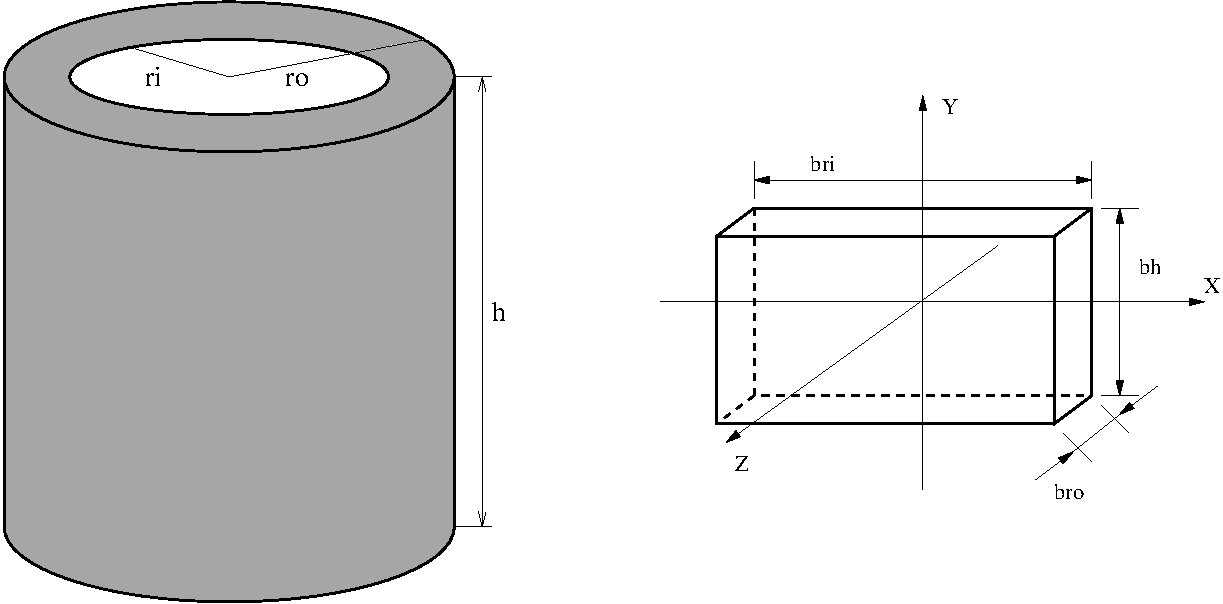
\includegraphics[width=0.9\textwidth]{figures/res_sample}
%    \caption{The two possible shapes of the \textbf{Res\_sample} component.}
%    \label{f:res_sample}
%  \end{center}
%\end{figure}
%
The component only propagates neutron rays that are scattered;
other rays are absorbed. The scattering probability is proportional to the neutron
flight path length inside the sample, to make a true volume weighting
of the sample. The reason for this is that the resolution
function of an instrument is independent of any sample properties
such as scattering and absorbtion cross sections but will in general
depend on sample size and shape.

The point of scattering inside the sample is chosen uniformly
along the neutron flight path inside the sample, and the scattered
neutron ray is given a random energy and direction. This energy is selected in
the interval $[E_0-\Delta E; E_0+\Delta E]$ which hence must be
chosen large enough to cover all interesting neutron energies.
Similarly, the scattered
direction is chosen in a user-specified range,
either within a sphere of radius $r_{\rm focus}$, within a rectangular
target with measures $(x_{\rm focus}, y_{\rm focus})$
or in the specified angular range. This target is positioned at the $x_{target}$, $y_{target}$, $z_{target}$ point in space, or using the target\_index for which e.g. 1 is the further component, -1 is the previous, etc...

A special feature, used when computing resolution functions, is that the
component stores complete information about the scattering event in the
output parameter \textit{res\_struct}. The information includes initial
and final wave vectors, the coordinates of the scattering point, and the
neutron weight after the scattering event. From this information the
scattering parameters $({\bf Q}, \omega)$ can be recorded
for every scattering event and used to compute the resolution function.
For an example of using the
information in the output parameter, see the description of the
\textbf{Res\_monitor} component in section~\ref{s:res_monitor}.



% Emacs settings: -*-mode: latex; TeX-master: "manual.tex"; -*-

\section{TOF\_Res\_sample: A sample-like component for TOF resolution calculation}
\label{s:tof_res_sample}

%\component{TOF\_Res\_sample}{System}{$r_\textrm{i}$, $r_\textrm{o}$, $h$, $r_\textrm{focus}$, $x_\textrm{target}$, $y_\textrm{target}$, $z_\textrm{target}$, $t_0$, $\Delta t$ }{$x_w$, $y_h$, $z_t$, $x_\textrm{focus}$, $y_\textrm{focus}$, $a_\textrm{v, focus}$, $a_\textrm{h, focus}$, target index}{}
\mcdoccomp{misc/TOFRes_sample.parms}

The component \textbf{TOF\_Res\_sample} scatters neutron rays isotropically
in position within a specified angular range. 
As for \textbf{Res\_sample}, this component is meant
for computation of the resolution function, but in this case for one time bin in a
time-of-flight (TOF) instrument. The component selects uniformly the neutron 
energy so that neutron arrival time at the TOF detector lies within one time bin,
specified by $t_0$ and $\Delta t$.
For actual calculations of the resolution
function, \textbf{TOF\_Res\_sample} should be used
together with \textbf{Res\_monitor}, described in
section~\ref{s:res_monitor}.

The shape of \textbf{TOF\_Res\_sample} is either a hollow cylinder
or a rectangular box. 
The hollow cylinder shape is
specified with the inner and outer radius, $r_\textrm{i}$ and $r_\textrm{o}$,
respectively, and the height, $h$.
If these parameters are unspecified,
the shape is instead a box of dimensions $x_w$, $y_h$, and $z_t$.
%See figure~\ref{f:res_sample}.\par

The component only propagates neutron rays that are scattered; 
other rays are absorbed. 
As for \textbf{Res\_sample}, the scattering probability is proportional to the neutron
flight path length inside the sample.
The point of scattering in the sample is chosen uniformly
along the neutron flight path inside the sample, and the scattered
direction is chosen in a user-specified range,
either within a sphere of radius $r_\textrm{foc}$, within a rectangular
target with measures $(x_\textrm{focus}, y_\textrm{focus})$
or in the specified angular range. 
This target is positioned at the $x_{target}$, $y_{target}$, $z_{target}$ 
point in space, or using target\_index.

This component stores complete information about the scattering event in the
output parameter \textit{res\_struct}, see \textbf{Res\_Sample}. 


\section{Res\_monitor: The monitor for resolution calculation}
\label{s:res_monitor}
\index{Monitors!Resolution monitor|see{Samples/Resolution function}}

%\component{Res\_monitor}{(System); Alan Tennant, HMI}{$x_{\rm min}$, $x_{\rm max}$, $y_{\rm min}$, $y_{\rm max}$, filename, res\_sample, buffer size}{$x_w$, $y_h$, $z_t$, options}{}
\mcdoccomp{misc/Res_monitor.parms}

The component {\bf Res\_monitor} is used for calculating the
resolution function of a particular instrument with detector of the
given shape, size, and position.
The shape of {\bf Res\_monitor} is by default rectangular,
but can be a box, a sphere, a disk, or a cylinder,
depending on the parameter ``options''.
The component works like a normal monitor, but
also records all scattering events and stores
them to a file that can later be read by 
the \MCS frontend tool \verb+mcresplot+.

For time-of-flight (TOF) instruments, {Res\_monitor} should be understood 
as giving the resolution of one time bin of the TOF-detector only; 
the bin properties being specified in the preceding {\bf TOF\_Res\_sample}.

As described in section~\ref{s:res_sample},
the {\bf Res\_monitor} should be used in connection with one of the
components {\bf Res\_sample} or {\bf TOF\_Res\_sample}, 
the name of which should be passed as an
input parameter to \textbf{Res\_monitor}. For example
\begin{lstlisting}
    COMPONENT mysample = Res_sample( ... )
    ...
    COMPONENT det = Res_monitor(res_sample_comp = mysample, ...)
    ...
\end{lstlisting}

The output file is in ASCII format, one line per scattering event, with
the following columns:
\begin{itemize}
\item ${\bf k}_{\rm i}$, the three components of the initial wave vector.
\item ${\bf k}_{\rm f}$, the three components of the final wave vector.
\item ${\bf r}$, the three components of the position of the scattering
  event in the sample.
\item $p_{\rm i}$, the neutron weight just after the scattering event.
\item $p_{\rm f}$, the relative neutron weight adjustment from sample to
  detector (so the total weight in the detector is $p_{\rm i}p_{\rm f}$).
\end{itemize}
From ${\bf k}_{\rm i}$ and ${\bf k}_{\rm f}$, we may compute 
the scattering parameters 
$\kappa = {\bf k}_{\rm i} - {\bf k}_{\rm f}$ and 
$\hbar \omega = \hbar^2/(2 m_{\rm n})({\bf k}_{\rm i}^2 - {\bf k}_{\rm f}^2)$.
The vectors are given in the local coordinate system of the resolution
sample component. The wave vectors are in units of $\mbox{\AA}^{-1}$, the
energy transfer in meV.

The output parameters from {\bf Res\_monitor}
are the three count numbers, \textit{Nsum}, \textit{psum},
and \textit{p2sum}, and the handle \textit{file} of the output file.


\newpage
\section{Progress\_bar: Simulation progress and automatic saving}
\component{Progress\_bar}{System}{percent, flag\_save, profile}{}{}
\label{s:progress-bar}
\index{Simulation progress bar}

This component displays the simulation progress and status
but does not affect the neutron parameters.
The display is updated in regular intervals of the full simulation;
the default step size is 10 \%, but it may be changed using
the \verb+percent+ parameter (from 0 to 100).
The estimated computation time is displayed at the begining
and actual simulation time is shown at the end.

Additionally, setting the \verb+flag_save+ to 1 results in
a regular save of the data files during the simulation.
This means that is is possible to view the data before the end
of the computation, and have also a trace of it in case of
computer crash. The achieved percentage of the simulation is stored in these temporary
data files. Technically, this save is equivalent to sending regularly
a USR2 signal to the running simulation.

The optional 'profile' parameter, when set to a file name, will produce the number of statistical events reaching each component in the simulation. This may be used to identify positions where events are lost.

\section{Beam\_spy: A beam analyzer}
\component{Beam\_spy}{System}{}{}{should overlap previous component}
\index{Monitors!Beam analyzer}

This component is at the same time an Arm and a simple Monitor. It analyzes all neutrons reaching it, and computes statistics for the beam, as well as the intensity.

This component does not affect the neutron beam, and does not contain any propagation call. Thus it gets neutrons from the previous component in the instrument description, and should better be placed at the same position, with \verb+AT (0,0,0) RELATIVE PREVIOUS+.


\appendix
% Loads of preamble stripped off - now located in mcstas.tex

%\newpage
\chapter{Polarization in McStas}
\label{c:polarization}
\begin{center}
\Large{P. Christiansen (Ris{\o})\\\today}
\end{center}

\section{Introduction}

In the current release of McStas there are components with polarization
capabilities. At the moment all such components should be understood as under
development as the amount of testing and debugging of these components is
small, and there are known problems.

Here, we shall report on what have been done so far.

We first describe the polarization vector and how it is related to the neutron
wave-function (section~\ref{sec:pol}) and then the physics of simple
components that we need in McStas is reviewed (section~\ref{sec:scat}). In the
last two sections the actual McStas polarization components are first
described (section~\ref{sec:new}) and a list of test instruments in McStas is
given (section~\ref{sec:test}).

We rely heavily on the books~\cite{lovesey84,gavin} for the physics where
the detailed calculations can be found.

The notation used here (and in~\cite{gavin}) is $P$ (scalar), $\PB$
(vector), $\tP$ (unit-vector), $\sigmaH$ (operator), and $\sigmao$
(vector of operators).

\section{The Polarization Vector}
\label{sec:pol}

The spin of the neutron is represented by an operator $\so$ for which only a
single component can be measured at one time. Each single measurement will
give a value $\pm 1/2$, but if we could make a large number of measurements on
the same neutron state, in each of the three axis directions, and then make
the average we get $\langle \so \rangle$. The polarization vector, $\PB$, is
then defined as:
\begin{equation}
  \label{eq:pol_single}
  \PB = \frac{\langle \so \rangle}{s},
\end{equation}
so that $-1 \leq |\PB| \leq +1$

For a neutron beam which contains $N$ neutrons, each with a
polarization $\PB_i$, the beam polarization is defined as:
\begin{equation}
  \label{eq:pol_beam}
  \PB = \frac{\sum_i \PB_i}{N}.
\end{equation}

If we have one common quantization direction (e.g. a magnetic field
direction) each neutron will either be spin up, $\uparrow$, or spin down,
$\downarrow$, and the polarization can be expressed as:

\begin{equation}
  \label{eq:pol}
  P = \frac{\nup-\nd}{\nup+\nd},
\end{equation}

where $\nu$ ($\nd$) is the number of neutrons with spin up
(down).

For a given neutron the probability of the neutron being spin up, $\Pu$, is:

\begin{equation}
  \label{eq:prob_spinup}
  \Pu = \frac{\nup}{\nup+\nd} = \frac{\nup + (\nd-\nd)/2}{\nup+\nd}
  = \frac{1+P}{2},
\end{equation}

and $\Pd = 1-\Pu = (1-P)/2$.

The expectation value of the 'spin' operator, $\sigmao$, which can be
expressed by the Pauli matrices, is the polarization vector $\PB$, $\PB =
\langle \sigmao \rangle \equiv \langle \chi | \sigmao | \chi \rangle$.  The
most general form of the spin wave-function $\chi$ for a neutron (spin 1/2)
is:

\begin{equation}
  \label{eq:neutron_wave}
  \chi = a\chi_\uparrow + b\chi_\downarrow,
\end{equation}

where $\chi_\uparrow$ and $\chi_\downarrow$ are eigenfunction of
$\hat{\sigma}^z$, and the complex coefficients $a$ and $b$ satisfy
$|a|^2 + |b|^2 = 1$.

By calculation we find:
\begin{eqnarray}
P_x & = & \langle \chi | \sigmaH_x | \chi \rangle
= 2 \text{Re}(a^\ast b) \\
P_y & = & \langle \chi | \sigmaH_y | \chi \rangle
= 2 \text{Im}(a^\ast b) \\
P_z & = & \langle \chi | \sigmaH_z | \chi \rangle
= |a|^2-|b|^2
\end{eqnarray}

This shows the relation of the polarization vector to the neutron wave
function.

The neutron magnetic moment operator can be expressed in terms of $\sigmao$,
as:
\begin{equation}
  \label{eq:magnetic}
  \muno = \mu_n \sigmao,
\end{equation}
which, as shown above, is related to the polarization vector.  \\

In our simulation we represent the polarization by the vector $\SB = (s_x,
s_y, s_z)$ which is propagated through the different components so it has the
correct relative orientation in each component. The probability for the spin
to be parallel a given direction $\mathbf{n}$ is then:

 \begin{equation}
   \label{eq:probmcstas}
   P(\uparrow|\nB) = \frac{1+\nB \cdot \SB}{2}.
 \end{equation}

This equation (from~\cite{pol_seeger}) is easy to understand. The
average spin along $\nB$ is $\nB \cdot \SB$ and the probability then
follows from Eq.~\ref{eq:prob_spinup}.

For an unpolarized beam, $\mathbf{S} = \mathbf{0}$ and all directions
are equally probable (50~\%).

Note that in our approach we do not decide if the neutron is up or down after
a given component, but instead keep track of as much information for as long
as possible.

In the following we will use $\PB$ to denote the polarization
vector. The most important variables used are:

\begin{tabular}{ll}

  $\Q$  & Scattering vector. \\
  $\PB$  & Polarization before a component (ingoing). \\
  $\PB_\perp$  & Polarization perpendicular to scattering vector,
  $\PB_\perp = \tQ \times (\PB \times \tQ$). \\
  $\PB'$ & Polarization after a component (outgoing). \\
  $\tN$ & Unit vector in direction of atomic spin ($\tN \cdot \tilde{\BB} = -1$ for a ferromagnet). \\
  $\FN$ & Unit cell nuclear structure factor. \\
  $\FM$ & Unit cell magnetic structure factor. \\
\end{tabular}
\\

The unit cell nuclear structure factor is defined as:

\begin{equation}
  \FN = \sum_\dB
  \exp(i\Q \cdot \dB)\overline{b}_d,
\end{equation}

where the $\dB$ is the position of the d'th atom within the unit cell,
and $\overline{b}_d$ is the average of $b_d$. In the simple case of a
single atom Bravais crystal one finds $\FN = \overline{b}$.

The unit cell magnetic structure factor is useful when the atoms in
the crystal only have spin orbital angular momentum, and simple when
the magnet is saturated (all spins are parallel or anti-parallel to
\emph{one} direction, $\sigma_d=\pm1$). It is then given as:

\begin{equation}
  \FM =
  \gamma_n r_0 \sum_\dB \exp(i\Q \cdot \dB)\frac{1}{2}g_d F_d(\Q)\langle
  \hat{S}_d\rangle \sigma_d,
\end{equation}

where $r_0=\frac{\mu_0}{4\pi}\frac{e^2}{m_e} = 2.818 \times 10^{-15}$m, $g=2$ is the
Land{\'e} splitting factor, and $F_d(\Q)$ is the magnetic form factor, which
is the Fourier transform of the magnetization density (normalized so that
$F_d(0) = 1$), and $\langle \hat{S}_d\rangle$ is the thermal average of the
ordered atomic spin.

In the following the Debye-Weller factor ($\exp(-W_d)$) have been ignored in
all cross sections.

\subsection{Example: Magnetic fields}

The magnetic moment operator of the neutron is $\muno = \gamma_n \so$, where
$\gamma_n = 2 \mu_n = -3.826$ is the gyromagnetic ratio (spin and magnetic
moment is anti-parallel as for an electron)~\footnote{Note that if we had used
S (with values $S=\pm 1$) to define $\gamma_n$ we would get $\gamma_n =
-1.913$ which is also commonly used.}

A magnetic field, $\BB$, will exert a torque, $\tauB = d\sB/dt = (1/\gamma_n)d\muB/dt$, on the neutron magnetic moment:

\begin{equation}
  \label{eq:torque}
  \frac{1}{\gamma_n} \frac{d\muB}{dt} = \muB \times \BB
\end{equation}

The magnetic moment $\mu$ can be related to the polarization as $\muB
= \gamma_n \PB/2$, and inserting in Eq.~\ref{eq:torque} we find:

\begin{equation}
  \label{eq:pol_magnetic}
  \frac{d\PB}{dt} = \gamma_n \PB \times \BB
\end{equation}

In the simple case where $\BB = (0, 0, B)$, we find the solution
(\cite{gavin} p.~18) :

\begin{eqnarray}
  \nonumber
  P_X(t) & = & \cos(\omega_L t) P_X(0) - \sin(\omega_L t) P_Y(0) \\
  \label{eq:precession}
  P_Y(t) & = & \sin(\omega_L t) P_X(0) + \cos(\omega_L t) P_Y(0) \\
  \nonumber
  P_Z(t) & = & P_Z(0),
\end{eqnarray}

where $\omega_L = -\gamma_n B/\hbar$ is the Larmor frequency.\\

\begin{quote}
  The equations above was checked against the equations in the ``polarimetrie
  neutronique'' notes by Francis Tasset and found to be consistent. There can
  be sign differences between different publications depending on whether they
  use a right-handed (like e.g. McStas) or a left-handed (like e.g. NISP)
  coordinate system.
\end{quote}

\section{Polarized Neutron Scattering}
\label{sec:scat}

First we will give a short introduction to how calculations are done
and then quote some results which are important for implementing the
first McStas components.

All the potentials (nuclear, magnetic, and electric) we will be interested in
can be written on the form:
\begin{equation}
  \label{eq:general_pot}
  \hat{v} = \betao + \alphao \cdot \sigmao
\end{equation}

The first term does not affect the spin, while the second term can
change the spin. Let us just remind here that:

\begin{equation}
  \label{eq:pauli_rules}
  \begin{matrix}
    \sigmaH_x \chiU = \chiD, &
    \sigmaH_y \chiU = i\chiD, &
    \sigmaH_z \chiU = \chiU, \\
    \sigmaH_x \chiD = \chiU, &
    \sigmaH_y \chiD = -i\chiU, &
    \sigmaH_z \chiD = -\chiD.
  \end{matrix}
\end{equation}

So that the interaction proportional to $\sigmaH_x$ and $\sigmaH_y$
results in spin flips, while the interactions with $\sigmaH_z$
conserves the spin.

It turns out to be smart to define a density matrix operator:
\begin{equation}
  \rhoo = \chi \chi^\dagger =
  \left( \begin{matrix}
    |a|^2 & ab^\ast \\
    ba^\ast & |b|^2
  \end{matrix} \right)
  = \frac{1}{2}({\cal I}+\PB \cdot \sigmao),
\end{equation}
where $\chi$ is the neutron wave function (Eq.~\ref{eq:neutron_wave}),
and ${\cal I}$ is the unit matrix.

Using the density matrix the elastic cross section can be written as
(\cite{lovesey84}, Eq.~10.31):
\begin{equation}
  \label{eq:master_sigma}
  \frac{d\sigma}{d\Omega} = \text{Tr} \rhoo \hat{v}^\dagger \hat{v}
  = \sum_{\lambda, \lambda'} p_\lambda \text{Tr} \rhoo
  \langle \lambda | \hat{V}^\dagger(\Q) | \lambda' \rangle
  \langle \lambda' | \hat{V}(\Q) | \lambda \rangle
  \delta(E_\lambda - E_{\lambda'}),
\end{equation}

where $\hat{V}$ is the interaction potential and it is understood that
the trace is to be taken with respect only to the neutron spin
coordinates. The outgoing polarization is given as:
\begin{equation}
  \label{eq:master_pol}
  \PB' \frac{d\sigma}{d\Omega} =
  \text{Tr} \rhoo \hat{v}^\dagger \sigmao \hat{v}
  = \sum_{\lambda, \lambda'} p_\lambda \text{Tr} \rhoo
  \langle \lambda | \hat{V}^\dagger(\Q) | \lambda' \rangle
  \sigmao
  \langle \lambda' | \hat{V}(\Q) | \lambda \rangle
  \delta(E_\lambda - E_{\lambda'})
\end{equation}

Inserting Eq.~\ref{eq:general_pot} in Eq.~\ref{eq:master_sigma} and
Eq.~\ref{eq:master_pol} results in the two master equations for
polarized neutron scattering:

\begin{equation}
  \label{eq:general_sigma}
  \text{Tr} \rhoo \hat{v}^\dagger \hat{v} =
  \alphao^\dagger \cdot \alphao + \betao^\dagger \betao+
  \betao^\dagger (\alphao \cdot \PB) +
  (\alphao^\dagger \cdot \PB) \betao +
  i\PB \cdot (\alphao^\dagger \times \alphao),
\end{equation}

and

\begin{equation}
  \label{eq:general_pol}
  \text{Tr} \rhoo \hat{v}^\dagger \sigmao \hat{v} =
  \betao^\dagger \alphao
  + \alphao^\dagger \betao
  + \betao^\dagger \betao \PB
  + \alphao^\dagger (\alphao \cdot \PB)
  + (\alphao^\dagger \cdot \PB) \alphao
  - \PB (\alphao^\dagger \cdot \alphao)
  - i \alphao^\dagger \times \alphao
  + i \betao^\dagger (\alphao \times \PB)
  + i (\PB \times \alphao^\dagger) \betao.
\end{equation}

Based on these two equations and the interaction potentials all the
results presented in the following are derived in~\cite{lovesey84}.

\subsection{Example: Nuclear scattering}

The nuclear scattering potential for a crystal is:
\begin{equation}
  \label{eq:nuclear_pot}
  \hat{V}_N(\Q) = \sum_{\lB,\dB} \exp(i\Q \cdot \RB_{ld})(A_{ld} +
  \frac{1}{2} B_{ld} \sigmao \cdot \Io_{ld}),
\end{equation}

so that

\begin{eqnarray}
  \label{eq:ab_nuclear}
  \alphao & = &
  \sum_{\lB,\dB} \exp(i\Q \cdot \RB_{ld}) \frac{1}{2} B_{ld} \Io_{ld} \\
  \betao & = &
  \sum_{\lB,\dB} \exp(i\Q \cdot \RB_{ld}) A_{ld},
\end{eqnarray}

where $\Io$ is the nuclear spin operator and the constants $A$ and $B$
are related to the nuclear scattering lengths $b^+$ and $b^-$ as
$A=((I+1)b^++Ib^-)/(2I+1)$ and $B=(b^++b^-)/(2I+1)$.

To calculate the polarization cross section and outgoing polarization
we have to average over the nuclear spin (which we assume is random
oriented), so that terms linear in $\alphao$ (three last terms in
Eq.~\ref{eq:general_sigma}) disappears. The scattering cross section
ends up being (see~\cite{lovesey84} p.~159):

\begin{equation}
  \label{eq:nuclear_sigma}
  \frac{d\sigma}{d\Omega}  =
  \sum_{\lB, \dB, \lB', \dB'} \exp(i \Q \cdot (\RB_{ld}-\RB_{l'd'}))
  (\madsq + \delta_{\lB,\lB'}\delta_{\dB,\dB'}[\sqmad - \madsq
  + \frac{1}{4}\bd])
\end{equation}

where the first term is the coherent cross-section and the second term is the
site-incoherent cross-section. Both terms are independent of $\PB$ as expected
for a system without a preferred internal direction.

The polarization in the final state is:

\begin{equation}
  \label{eq:nuclear_pol}
  \PB' \frac{d\sigma}{d\Omega}  =
  \sum_{\lB, \dB, \lB', \dB'} \exp(i \Q \cdot (\RB_{ld}-\RB_{l'd'}))
  \PB' (\madsq + \delta_{\lB,\lB'}\delta_{\dB,\dB'}[\sqmad - \madsq
  - \frac{1}{12}\bd])
\end{equation}

Comparing Eq.~\ref{eq:nuclear_sigma} and Eq.~\ref{eq:nuclear_pol} we
find that: 1) The nuclear coherent polarization is the same as the
initial polarization. 2) The same is true for the incoherent
scattering due to the random isotope distribution. 3) The nuclear
incoherent scattering due to the random nuclear spin orientations has
polarization $\PB' = -1/3 \PB$ (for a random nuclear spin the
associated Pauli matrix will 2/3 of the time point in the direction of
$\sigmaH_x$ and $\sigmaH_y$ which according to
Eq.~\ref{eq:pauli_rules} flips the spin). \\

For Vanadium, where there is only one isotope and coherent scattering
is negligible, we find $\PB' = -1/3\PB$. There is however one
catch. If the probability for multiple scattering is large one has to
take into account that after two scattering one has: $\PB'(2) =
1/9\PB$, and so forth. The average polarization after a thick vanadium
target is therefore a sum of different contributions.

\subsection{Example: Polarizing Monochromator and Guides}
\label{sub:mono}

\begin{figure}[htbp]
  \begin{center}
    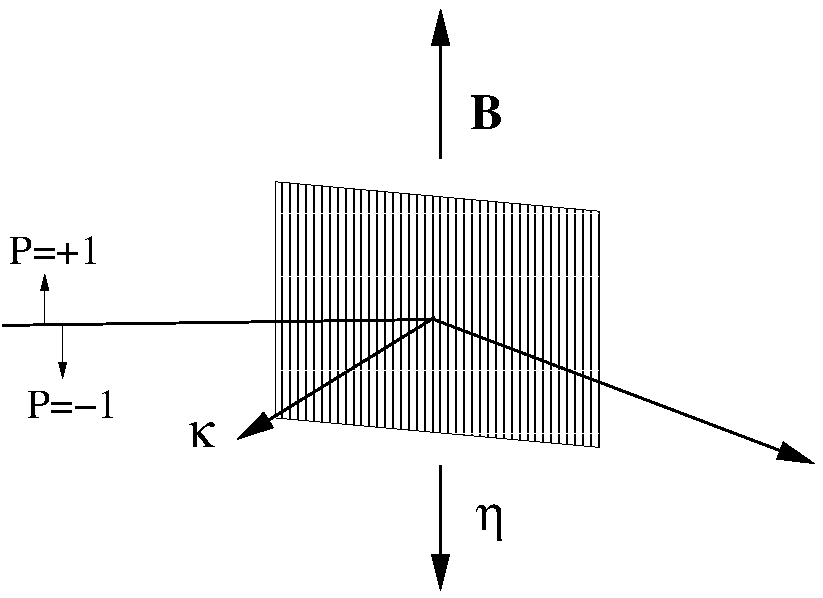
\includegraphics[keepaspectratio,
    width=0.7\columnwidth]{figures/monochromator_pol}
    \caption{Principle and geometry of a polarizing monochromator.}
    \label{fig:mono_princip}
  \end{center}
\end{figure}

In a polarized monochromator and polarizing guides we have a ferromagnetic
crystal in an external magnetic field. The scattering potential is now both
nuclear (no internal direction) and magnetic (internal direction), so in
general the outgoing polarization can be quite complex. However, as
illustrated in Figure~\ref{fig:mono_princip}, the typical setup has many
geometrical constraints: $\tN \cdot \tQ = 0$, $\tN \cdot \PB_\perp = \tN \cdot
\PB$, and $\Q \times (\tN \times \Q) = \tN$, which simplifies the problem.

In~\cite{lovesey84} the calculation for a centrosymmetric ferromagnetic
crystal is done, and inserting the constraints above one finds
(\cite{lovesey84}, Eq.~10.96 and Eq.~10.110):

\begin{eqnarray}
  \label{eq:mono_sigma}
  d\sigma/d\Omega & = & \FN^2 + 2\FN\FM (\PB \cdot \tN) + \FM^2\\
  \label{eq:mono_pol}
  \PB' d\sigma/d\Omega & =
  & \PB [\FN^2 - \FM^2] + \tN [2\FN\FM + 2(\tN \cdot \PB)\FM^2]
\end{eqnarray}

\begin{quote}
  NB! Note that in~\cite{gavin} Eq.~2.2.25 there is a minus in front of the
  second term in Eq.~\ref{eq:mono_sigma}. We have not been able to understand
  this discrepancy, which is probably due to notation. Most other authors
  agree with the minus in front of the second term (e.g. Squires and Francis
  Tasset).
\end{quote}

For a beam which is initially unpolarized we find the outgoing
polarization to be:
\begin{equation}
  \PB' = \frac{\tN 2\FN \FM}{d\sigma/d\Omega}
  = \frac{2\FN\FM}{\FN^2 + \FM^2} \tN,
\end{equation}

so that the beam is fully polarized along $\tN$ if $\FN = \pm \FM$. \\

What we use to characterize the polarizing monochromator in practice
is not $\FN$ and $\FM$, but instead the reflection probabilities $\Ru$
and $\Rd$ (for the reflection of interest).

If we assume that the reflection probabilities are directly proportional to
the cross sections (with proportionality constant $k$), i.e., $\Ru = k
d\sigma/d\Omega(\PB=+\tN)$ and $\Rd = k d\sigma/d\Omega(\PB=-\tN)$ then we can
use Eq.~\ref{eq:mono_sigma} to determine $\FN$ and $\FM$:

\begin{eqnarray}
  \label{eq:mono_up}
  \Ru & = & k (\FN + \FM)^2,\\
  \label{eq:mono_down}
  \Rd & = & k (\FN - \FM)^2.
\end{eqnarray}

The values of $\sqrt{k}\FN$ and $\sqrt{k}\FM$ are then between -1 and +1 and
unit less like the reflection probabilities. In the following we ignore $k$ and
just talk about $\FN$ and $\FM$.

In principle there are four solutions for $\FN$ and $\FM$, so in the code we
currently choose the values where $\FN + \FM = +\sqrt{\Ru}$ and $\FN - \FM =
+\sqrt{\Rd}$ (so that $\FN>0$ and $\FN>\FM$). We then find:

\begin{eqnarray}
  \label{eq:mono_nuc}
  \FN & = & \frac{\sqrt{\Ru} + \sqrt{\Rd}}{2},\\
  \label{eq:mono_mag}
  \FM & = & \frac{\sqrt{\Ru} - \sqrt{\Rd}}{2}.
\end{eqnarray}

When $\FN$ and $\FM$ are determined from these equations,
Eq.~\ref{eq:mono_sigma} and Eq.~\ref{eq:mono_pol} can easily be used to handle
any situation.

This solution is both used for monochromators and guides.

It is not clear that this solution is correct. If we make a simple example
with $\Ru = 1$ and $\Rd = 0.25$ then we could in principle have four
solutions, but let us just quote the two where $\FN$ is positive since the
last two are found by inserting a minus before all the solutions and this does
not change the physics. The two solutions are $\FN = 0.75, \FM=0.25$ and $\FM
= 0.75, \FN=0.25$. All solutions gives the same cross section, but if the
incoming beam is polarized (and only then) the outgoing beam will have two
different polarization values, since $\PB [\FN^2 - \FM^2]$ and $\tN 2(\tN
\cdot \PB)\FM^2$ are different for the two solutions. It seems that one needs
some additional information to choose between the two solutions.

\begin{quote}
  NB! The simplifying geometry shown in Figure~\ref{fig:mono_princip} only
  applies for the sides of the guide wall and not the top and bottom (assuming
  that the magnetizing field is pointing up or down), so there another set of
  equations should really be used.
\end{quote}

The same physics could also be used for a polarizing powder or single crystal
sample if $\FN$ and $\FM$ can be calculated with some other program, but one
would have to use the general form of Eq.~\ref{eq:mono_sigma} and
Eq.~\ref{eq:mono_pol} without the simplifying geometrical constraints for
monochromators and guides.

\section{New McStas Components}
\label{sec:new}

The components written so far can be divided into four groups:
\begin{itemize}
\item \textbf{Polarizers:} Components used to make the beam polarized.
\item \textbf{Monitors:} Unphysical detectors that can measure the polarization
of the neutrons.
\item \textbf{Magnetic fields:} Components used to handle magnetic fields.
\item \textbf{Samples:} Samples that affects the polarization.
\end{itemize}

\subsection{Polarizers}

Some of the most common ways of polarizing a beam have been
implemented.

\begin{itemize}
\item \textbf{Set\_pol:} This unphysical component can be used in two
ways. Either to hard code the polarization to the vector $(px, py, pz)$
or when randomOn!=0 to set the polarization vector to a random vector
on the unit sphere.\\

\item \textbf{Monochromator\_pol:} A monochromator that only does the $n=1$
  reflection. For each neutron it calculates the wavelength which would give
  Bragg reflection, $\lambda_\text{Bragg}$, and it then calculates, based on
  one mosaicity and one d-spread, the reflection probability given the neutrons
  actual $\lambda$.  The reflection probability is a Gaussian in $\Delta
  \lambda = \lambda - \lambda_\text{Bragg}$, with the peak reflectivity and
  polarization calculated as described in section~\ref{sub:mono}.

  \begin{quote}
    NB! Note that this monochromator reflects the neutrons billiard-like. In
    \textbf{Monochromator\_flat} the mosaicity of the reflecting crystal is
    taken into account, but the d-spread is not taken into account. One should
    implement d-spread and mosaicity in a way similar to what is done in
    \textbf{Single crystal}.
  \end{quote}

\item \textbf{Pol\_mirror:} Plane with a reflection probability for up
and down. There are 3 options: always reflect, always transmit, or
random select transmit/reflect.

\begin{quote}
  NB! Note that at the moment the plane only reflects from one side (because
  it uses PROP\_Z0.
\end{quote}

\item \textbf{Pol\_bender:} Curved guide with the possibilities to
  insert multiple slits, and have the end gap parallel to the entrance
  or following the guide angle. It is possible to select different
  coatings (mirror parameters) for each of the four sides.\\

\item \textbf{Pol\_guide\_vmirror:} Straight guide with non-polarizing
  coatings with two polarizing super mirrors sitting in a V shape
  inside. \\
\end{itemize}

Note that for all the polarizing guides it is possible to define analytical
functions or use tables for the up and down reflectivity descriptions.

\subsection{Detectors}

\begin{itemize}
\item \textbf{Pol\_monitor:} One defines a vector $\mathbf{m} = (mx,
  my, mz)$ for the monitor and measures the projection of the spin
  along this vector i.e. $\mathbf{m} \cdot \mathbf{S}$.\\

\item \textbf{PolLambda\_monitor:} Measures the projection of the
  spin along the defined vector $\mathbf{m}$ (see
  \textbf{Pol\_monitor}) as a function of the wavelength $\lambda$.

\item \textbf{MeanPolLambda\_monitor:} Measures the \emph{average}
  projection of the spin along the defined vector $\mathbf{m}$ (see
  \textbf{Pol\_monitor}) as a function of the wavelength $\lambda$.

  \begin{quote}
    NB! currently the error on the mean is shown ($\sigma/\sqrt(N)$), but it
    might make more sense to show the spread ($\sigma$).
  \end{quote}
\end{itemize}

\subsection{Magnetic fields}

Much inspiration for the components and the tests have been found
in~\cite{pol_seeger}.

\begin{itemize}
\item \textbf{Pol\_constBfield:} A rectangular box with a constant magnetic
  field in the y-direction. The x- and z-components of the spin precess with
  the Larmor frequency $\omega_L$. It is possible to define the field in terms
  of a wavelength so that the spin will precess 180 degrees for the given
  wavelength. The component can be rotated to have the field along another
  axis. \\

\item \textbf{Pol\_simpleBfield:} The first attempt at a component for
  handling general magnetic fields. It is a concentric component where you
  define a start and stop component for each field, but this allows other
  components, e.g. monitors, to be put inside the field. The component
  overloads the propagation routines so that numerical spin propagation is
  done for analytical magnetic fields.

  \begin{quote}
    NB! At the moment both components does not really check the boundaries of
    the field on the sides, but merely assumes that the field starts at the
    entrance plane and stops at the exit plane.

    Also, some optimization remains for the numerical component and it would
    be nice to support tabulated magnetic field files. However, the framework
    developed for \textbf{Pol\_simpleBfield} is very general and should
    easily facilitate these changes.
  \end{quote}

\end{itemize}


\subsection{Samples}

\begin{itemize}
\item \textbf{V\_sample:} Modified the sample so that the scattered
  neutron has $\PB' = -1/3\PB$. Note that this component does not
  handle multiple scattering, so this approach is correct. If the
  components handled multiple scattering the polarization should be
  set to $\PB' = (-1/3)^n\PB$, where $n$ is the number of
  scatterings.\\
\end{itemize}


\section{Tests With New Components}
\label{sec:test}

All the test instruments can be found in the McStas examples folder
(go to ``Neutron site/tests'' in mcgui).

There are basically two kind of tests. The first kind of tests shows
that the polarizing component can reproduce the same results as a
similar non-polarizing component:
\begin{itemize}
\item \textit{Test\_Monochromators.instr} : Intercomparison of
  \textbf{Monochromator\_flat} and \textbf{Monochromator\_pol}.
\item \textit{Test\_Pol\_Bender\_Vs\_Guide\_Curved.instr} : Intercomparison of
  \textbf{Guide\_curved} and \textbf{Pol\_bender}.
\end{itemize}

The second type of test illustrates the polarizing capabilities of the
component:
\begin{itemize}
\item \textit{Test\_Magnetic\_Constant.instr} : Constant magnetic field.
\item \textit{Test\_Magnetic\_Majorana.instr} : Linearly decreasing field with
  small transverse component.
\item \textit{Test\_Magnetic\_Rotation.instr} : Rotating magnetic field.
\item \textit{Test\_Magnetic\_Userdefined.instr} : Example of how to make a
  user defined analytic magnetic field that can also depend on time.
\item \textit{Test\_Pol\_Bender.instr} : Illustrates beam polarization with
  the \textbf{Pol\_bender}.
\item \textit{Test\_Pol\_Set.instr} : Tests \textbf{Pol\_set}.
\item \textit{Test\_Pol\_Guide\_Vmirror.instr} : Illustrates beam polarization
  with the \textbf{Pol\_guide\_vmirror}.
\item \textit{Test\_Pol\_Mirror.instr} : Illustrates beam polarization
  with the \textbf{Pol\_mirror}.
\item \textit{Test\_Pol\_TripleAxis.instr} : An example of a triple axis
  spectrometer with polarizing monochromators, a vanadium sample, and a spin
  flipper.
\end{itemize}


% Emacs settings: -*-mode: latex; TeX-master: "manual.tex"; -*-

\chapter{Libraries and conversion constants}
\label{c:kernelcalls}
\index{Library|textbf}
\index{Library!Shared|see{Library/Components/share}}
\index{Library!mcxtrace-r|see{Library/Run-time}}

The \MCX\ Library contains a number of built-in functions
and conversion constants which are useful when constructing
components. These are stored in the \verb+share+ directory of
the \verb+MCXTRACE+ library. \index{Library!Components!share}
\index{Environment variable!MCXTRACE}

Within these functions, the 'Run-time' part is available for all
component/instrument descriptions. The other parts
% (see table~\ref{t:comp-share})
are dynamic, that is they are not
pre-loaded, but only imported once when a component requests it
using the \verb+%include+ \MCX keyword. For instance, within a
component C code block, (usually SHARE or DECLARE):
\index{Keyword!\%include}
\begin{lstlisting}
    %include "read_table-lib"
\end{lstlisting}
will include the 'read\_table-lib.h' file, and the 'read\_table-lib.c'
(unless the \verb+--no-runtime+ option is used with \verb+mcxtrace+).
Similarly,
\begin{lstlisting}
    %include "read_table-lib.h"
\end{lstlisting}
will \emph{only} include the 'read\_table-lib.h'.
The library embedding is done only once for all components (like the
 SHARE section). \index{Keyword!SHARE} For an example
of implementation, see {\bfseries Res\_monitor}.

In this Appendix, we present a short list of both each of the library contents
and the run-time features.

\section{Run-time calls and functions (\texttt{mcxtrace-r})}
\label{s:calls:run-time}
\index{Library!Run-time|textbf}
\index{Library!mcxtrace-r|see{Library/Run-time}}
Here we list a number of preprogrammed macros and functions
which may ease the task of writing component and instrument definitions.
By convention macros are in upper case whereas functions are in lower case.

\subsection{Photon propagation}
\index{Library!Run-time!SCATTER}
\index{Library!Run-time!ABSORB}
\index{Library!Run-time!PROP\_Z0}
\index{Library!run-time!PROP\_X0}
\index{Library!run-time!PROP\_Y0}
\index{Library!Run-time!PROP\_DL}
\index{Library!Run-time!ALLOW\_BACKPROP}
Propagation routines perform all necessary operations to transport x-rays
from one point to an other. Except when using the special
\verb+ALLOW_BACKPROP;+ call prior to executing any \verb+PROP_*+ propagation,
the x-rays which have negative propagation lengths are removed automatically.
\begin{itemize}
\item {\bfseries ABSORB}. This macro issues an order to the overall
  \MCX\ simulator to interrupt the simulation of the current x-ray
  history and to start a new one.
\item {\bfseries PROP\_Z0}. Propagates the x-ray to the $z=0$ plane,
  by adjusting $(x,y,z)$, $\phi$, and $t$ accordingly from knowledge of the
  x-ray wavevector $(kx,ky,kz)$.
  If the propagation length is negative, the x-ray is absorbed, except if a \verb+ALLOW_BACKPROP;+ preceeds it.

  For components that are centered along the $z$-axis,
  use the \verb+_intersect+ functions to determine intersection time(s),
  and then a \verb+PROP_DL+ call.
\item {\bfseries PROP\_X0, PROP\_Y0}. These macros are analogous to \verb+PROP_Z0+ except they propagate to the $x=0$ and $y=0$ planes respectively.

\item {\bfseries PROP\_DL}$(dl)$. Propagates the x-ray by the length $dl$, adjusting $(x,y,z)$, $\phi$, $t$ accordingly,
  from knowledge of the x-ray wavevector.
\item {\bfseries ALLOW\_BACKPROP}. Indicates that the \emph{next} propagation routine
  will not remove the x-ray, even if negative propagation lengths
  are found. Subsequent propagations are not affected.\index{Removed x-ray events}
\item {\bfseries SCATTER}. This macro is used to denote a scattering event
  inside a component.
%, see section~\ref{s:comp-trace}.
  It should be used
  to indicate that a component has interacted with the x-ray
  (e.g. scattered or detected).
  This does not affect the x-ray state (see, however, {\bfseries Beamstop}),
  and it is mainly used by the \verb+MCDISPLAY+ section and the \verb+GROUP+ modifier.
%(see~\ref{s:trace} and \ref{s:comp-mcdisplay}).
  See also the SCATTERED variable (below).
  \index{Keyword!GROUP} \index{Keyword!MCDISPLAY} \index{Keyword!EXTEND}
\end{itemize}

\subsection{Coordinate and component variable retrieval}
\index{Library!Run-time!MC\_GETPAR}
\index{Library!Run-time!NAME\_CURRENT\_COMP}
\index{Library!Run-time!POS\_A\_CURRENT\_COMP}
\index{Library!Run-time!ROT\_A\_CURRENT\_COMP}
\index{Library!Run-time!POS\_A\_COMP}
\index{Library!Run-time!ROT\_A\_COMP}
\index{Library!Run-time!STORE\_XRAY}
\index{Library!Run-time!RESTORE\_XRAY}
\index{Library!Run-time!SCATTERED}
\begin{itemize}
\item {\bfseries MC\_GETPAR}$(comp, outpar)$. This may be used in e.g. the FINALLY section of an
  instrument definition to reference the parameters of a
  component.
% See page~\pageref{mcgetpar} for details.
\item {\bfseries NAME\_CURRENT\_COMP} gives the name of the current component as a string.
\item {\bfseries POS\_A\_CURRENT\_COMP} gives the absolute position of the
  current component. A component of the vector is referred to as
  POS\_A\_CURRENT\_COMP.$i$ where $i$ is $x$, $y$ or $z$.
\item {\bfseries ROT\_A\_CURRENT\_COMP} and
  {\bfseries ROT\_R\_CURRENT\_COMP} give the orientation
  of the current component as rotation matrices
  (absolute orientation and the orientation relative to
  the previous component, respectively). A
  component of a rotation matrix is referred to as
  ROT\_A\_CURRENT\_COMP$[m][n]$, where $m$ and
  $n$ are 0, 1, or 2 standing for $x,y$ and $z$ coordinates respectively.
\item {\bfseries POS\_A\_COMP}$(comp)$ gives the absolute position
  of the component with the name {\em comp}. Note that
  {\em comp} is not given as a string. A component of the
  vector is referred to as POS\_A\_COMP$(comp).i$
  where $i$ is $x$, $y$ or $z$.
\item {\bfseries ROT\_A\_COMP}$(comp)$ and
  {\bfseries ROT\_R\_COMP}$(comp)$ give the orientation of the
  component {\em comp} as rotation matrices (absolute
  orientation and the orientation relative to its
  previous component, respectively). Note that {\em comp}
  is not given as a string. A component of  a rotation
  matrice is referred to as
  ROT\_A\_COMP$(comp)[m][n]$, where $m$ and $n$ are
  0, 1, or 2.
\item {\bfseries INDEX\_CURRENT\_COMP} is the number (index) of the
       current component  (starting from 1).
\item {\bfseries POS\_A\_COMP\_INDEX}$(index)$ is the absolute position of
  component $index$. \\
  POS\_A\_COMP\_INDEX (INDEX\_CURRENT\_COMP) is the same as \\
  POS\_A\_CURRENT\_COMP. You may use \\
  POS\_A\_COMP\_INDEX  (INDEX\_CURRENT\_COMP+1) \\
  to make, for instance, your
  component access the position of the next component (this is usefull for
  automatic targeting).  A component of the vector is referred to as
  POS\_A\_COMP\_INDEX$(index).i$ where $i$ is $x$, $y$ or $z$.
\item {\bfseries POS\_R\_COMP\_INDEX} works the same as above,
  but with relative coordinates.
\item {\bfseries STORE\_XRAY}$(index, x, y, z, kx, ky, kz, phi,t, Ex, Ey,
Ez, p)$ stores the current x-ray state in the trace-history table,
in local coordinate system. $index$ is usually INDEX\_CURRENT\_COMP.
This is automatically done when entering each component of an
instrument.
\item {\bfseries RESTORE\_XRAY}$(index, x, y, z, kx, ky, kz, phi,t, Ex, Ey,
Ez, p)$ restores the x-ray state to the one at the input of the
component $index$. To ignore a component effect, use
RESTORE\_XRAY (INDEX\_CURRENT\_COMP, \\
$x, y, z, kx, ky, kz, phi,
Ex, Ey, Ez, p$) at the end of its TRACE section, or in its EXTEND
section. These x-ray states are in the local component coordinate
systems.
\item {\bfseries SCATTERED} is a variable set to 0 when entering
  a component, which is incremented each time a SCATTER event occurs.
  This may be used in the \verb+EXTEND+ sections to determine whether
  the component interacted with the current x-ray.
\item {\bfseries extend\_list}($n$, \&\textit{arr}, \&\textit{len},
  \textit{elemsize}). Given an array \textit{arr} with \textit{len}
  elements each of size \textit{elemsize}, make sure that the array is
  big enough to hold at least $n$ elements, by extending \textit{arr}
  and \textit{len} if necessary. Typically used when reading a list of
  numbers from a data file when the length of the file is not known in advance.
\item {\bfseries mcset\_ncount}$(n)$. Sets the number of x-ray histories to simulate to $n$.
\item {\bfseries mcget\_ncount}(). Returns the number of x-ray histories to simulate (usually set by option \verb+-n+).
\item {\bfseries mcget\_run\_num}(). Returns the number of x-ray histories that have been simulated until now.
\end{itemize}

\subsection{Coordinate transformations}
\begin{itemize}
\item {\bfseries coords\_set}$(x,y,z)$ returns a Coord structure (like POS\_A\_CURRENT\_COMP) with $x$, $y$ and $z$ members.
\item {\bfseries  coords\_get}$(P,$ \&$x$, \&$y$, \&$z)$ copies the $x$, $y$ and
$z$ members of the Coord structure $P$ into $x,y,z$ variables.
\item {\bfseries coords\_add}$(a,b)$, {\bfseries coords\_sub}$(a,b)$, {\bfseries
coords\_neg}$(a)$ enable to  operate on coordinates, and return the
resulting Coord structure.
\item {\bfseries rot\_set\_rotation}(\textit{Rotation t}, $\phi_x, \phi_y, \phi_z$)
  Get transformation matrix for rotation
  first $\phi_x$ around x axis, then $\phi_y$ around y,
  and last $\phi_z$ around z. $t$ should be a 'Rotation' ([3][3] 'double' matrix).
\item {\bfseries rot\_mul}\textit{(Rotation t1, Rotation t2, Rotation t3)} performs $t3 = t1 . t2$.
\item {\bfseries rot\_copy}\textit{(Rotation dest, Rotation src)} performs $dest = src$ for Rotation arrays.
\item {\bfseries rot\_transpose}\textit{(Rotation src, Rotation dest)} performs $dest = src^t$.
\item {\bfseries rot\_apply}\textit{(Rotation t, Coords a)} returns a Coord structure which is $t.a$
\end{itemize}

\subsection{Mathematical routines}
\begin{itemize}
\item {\bfseries NORM}$(x,y,z)$. Normalizes the vector $(x,y,z)$ to have
  length 1.
\item {\bfseries scalar\_prod}$(a_x,a_y,a_z, b_x,b_y,b_z)$. Returns the scalar
  product of the two vectors $(a_x,a_y,a_z)$ and $(b_x,b_y,b_z)$.
\item {\bfseries vec\_prod}(\&$a_x$,\&$a_y$,\&$a_z$, $b_x$,$b_y$,$b_z$, $c_x$,$c_y$,$c_z$). Sets
  $(a_x,a_y,a_z)$ equal to the vector product $(b_x,b_y,b_z) \times (c_x,c_y,c_z)$.
\item {\bfseries rotate}(\&$x$,\&$y$,\&$z$,$v_x$,$v_y$,$v_z$,$\varphi$,$a_x$,$a_y$,$a_z$). Set
  $(x,y,z)$ to the result of rotating the vector $(v_x,v_y,v_z)$
  the angle $\varphi$ (in radians) around the vector $(a_x,a_y,a_z)$.
\item {\bfseries normal\_vec}($n_x$, $n_y$, $n_z$, $x$, $y$, $z$).
  Computes a unit vector $(n_x, n_y, n_z)$ normal to the vector
  $(x,y,z)$.$^*$
\item {\bfseries solve\_2nd\_order}(*$t_0$,*$t_1$, $A$,  $B$,  $C$).
  Solves the 2$^{nd}$ order equation $At^2 + Bt + C = 0$ and puts the solutions in
  *$t_0$ and *$t_1$. The smallest positive solution into pointer *$t_0$. If $t_1$=\texttt{NULL}
  it is ignored and the second solution is discarded.
\end{itemize}

\subsection{Output from detectors}
Details about using these functions are given in the \MCX\ User Manual.
\begin{itemize}
\item {\bfseries DETECTOR\_OUT\_0D}$(...)$. Used to output the results from a
  single detector. The name of the detector is output together
  with the simulated intensity and estimated statistical error. The
  output is produced in a format that can be read by \MCX\ front-end
  programs.
%See section~\ref{s:comp-finally} ??? for details.
\item {\bfseries DETECTOR\_OUT\_1D}$(...)$. Used to output the results from a
  one-dimensional detector. Integrated intensities error etc. is also
  reported as for DETECTOR\_OUT\_0D.
%See section~\ref{s:comp-finally} for details.
\item {\bfseries DETECTOR\_OUT\_2D}$(\dots...)$. Used to output the results from a
  two-dimentional detector. Integrated intensities error etc. is also
  reported as for DETECTOR\_OUT\_0D.
%See section~\ref{s:comp-finally} for details.
%\item {\bfseries DETECTOR\_OUT\_3D}$(...)$. Used to output
%  the results from a three-dimentional detector. Arguments are the same as
%  in DETECTOR\_OUT\_2D, but with an additional $z$ axis.
%  Resulting data files are treated as 2D data, but the 3rd dimension is
%  specified in the $type$ field. Integrated intensities error etc. is also
%  reported as for DETECTOR\_OUT\_0D.
\item {\bfseries mcinfo\_simulation}\textit{(FILE *f, mcformat,
  char *pre, char *name)} is used to append the simulation parameters into file $f$
  (see for instance {\bfseries Res\_monitor}).
  Internal variable $mcformat$ should be used as specified.
  Please contact the authors for further information.
\end{itemize}

\subsection{Ray-geometry intersections}
\begin{itemize}
\item {\bfseries inside\_rectangle}($x$, $y$, $xw$, $yh$).
  Return 1 if $-xw/2 \leq x \leq xw/2$ AND $-yh/2 \leq y \leq yh/2$.
  Else return 0.
\item {\bfseries box\_intersect}(\&$l_1$, \&$l_2$, $x$, $y$, $z$, $k_x$, $k_y$, $k_z$,
  $d_x$, $d_y$, $d_z$). Calculates the (0, 1, or 2) intersections between
  the x-ray path and a box of dimensions $d_x$, $d_y$, and $d_z$,
  centered at the origin for a x-ray with the parameters
  $(x,y,z,k_x,k_y,k_z)$. The intersection lengths are returned
  in the variables $l_1$ and $l_2$, with $l_1 < l_2$. In the case
  of less than two intersections, $t_1$ (and possibly $t_2$) are set to
  zero. The function returns true if the x-ray intersects the box,
  false otherwise.
\item {\bfseries cylinder\_intersect}(\&$l_1$, \&$l_2$, $x$, $y$, $z$, $k_x$, $k_y$, $k_z$,
  $r$, $h$).  Similar to {\bfseries box\_intersect}, but using a cylinder of height $h$ and radius $r$,
  centered at the origin.
\item {\bfseries sphere\_intersect}(\&$l_1$, \&$l_2$, $x$, $y$, $z$, $k_x$, $k_y$, $k_z$,
  $r$). Similar to {\bfseries box\_intersect}, but using a sphere
  of radius $r$.
\item {\bfseries ellipsoid\_intersect}(\&$l_1$, \&$l_2$, $x$, $y$, $z$, $k_x$, $k_y$, $k_z$,
  $a$,$b$,$c$,$Q$, ). Similar to {\bfseries box\_intersect}, but using an ellipsoid with half-axis $a$,$b$,$c$ oriented by the rotation matrix $Q$.
  If $Q=I$, $a$ is along the $x$-axis, $b $ along $y$ and $c$ along $z$
\end{itemize}

\subsection{Random numbers}
By default  \MCX uses the included Mersenne Twister\cite{matsumoto1998mersenne} algorithm for generating pseudo random numbers.
\begin{itemize}
\item {\bfseries rand01}(). Returns a random number distributed uniformly between 0 and 1.
\item {\bfseries randnorm}(). Returns a random number from a normal
  distribution centered around 0 and with $\sigma=1$. The algorithm used to
  sample the normal distribution is explained in Ref.~\cite[ch.7]{num_rep}.
\item {\bfseries randpm1}(). Returns a random number distributed uniformly between -1 and 1.
\item {\bfseries randtriangle}(). Returns a random number from a triangular distribution between -1 and 1.
\item {\bfseries randvec\_target\_circle}(\&$v_x$, \&$v_y$, \&$v_z$, \&$d\Omega$,
  aim$_x$, aim$_y$, aim$_z$, $r_f$). Generates a random vector $(v_x, v_y,
  v_z)$, of the same length as (aim$_x$, aim$_y$, aim$_z$), which is
  targeted at a \emph{disk} centered at (aim$_x$, aim$_y$, aim$_z$) with
  radius $r_f$ (in meters), and perpendicular to the \emph{aim} vector.. All directions
  that intersect the circle are chosen with equal probability. The solid
  angle of the circle as seen from the position of the x-ray is returned
  in $d\Omega$. This routine was previously called {\bfseries randvec\_target\_sphere}
  (which still works).
\item {\bfseries randvec\_target\_rect\_angular}(\&$v_x$, \&$v_y$, \&$v_z$,
  \&$d\Omega$, aim$_x$, aim$_y$, aim$_z$,$h, w, Rot$) does the same as
  randvec\_target\_circle but targetting at a rectangle with angular dimensions
  $h$ and $w$ (in {\bfseries radians}, not in degrees as other angles). The
  rotation matrix $Rot$ is the coordinate system orientation in the absolute
  frame, usually ROT\_A\_CURRENT\_COMP.
\item {\bfseries randvec\_target\_rect}(\&$v_x$, \&$v_y$, \&$v_z$,
  \&$d\Omega$, aim$_x$, aim$_y$, aim$_z$,$height, width, Rot$) is the same as
  randvec\_target\_rect\_angular but $height$ and $width$ dimensions are given
  in meters. This function is useful to e.g. target at a guide entry window
  or analyzer blade.
\end{itemize}

\section{Reading a data file into a vector/matrix (Table input, \texttt{read\_table-lib})}
\label{s:read-table}
\index{Library!read\_table-lib (Read\_Table)|textbf}
  The \verb+read_table-lib+ library provides functionalities for reading text
  (and binary) data files. To use this library,
  add a \verb+%include "read_table-lib"+ in your component definition
  DECLARE or SHARE section. Tables are structures of type \verb+t_Table+
  (see \verb+read_table-lib.h+ file for details):
  \begin{lstlisting}[language=C]
    /* t_Table structure (most important members) */
    double *data;     /* Use Table_Index(Table, i j) to extract [i,j] element */
    long    rows;     /* number of rows */
    long    columns;  /* number of columns */
    char   *header;   /* the header with comments */
    char   *filename; /* file name or title */
    double  min_x;    /* minimum value of 1st column/vector */
    double  max_x;    /* maximum value of 1st column/vector */
\end{lstlisting}

Available functions to read \emph{a single} vector/matrix are:
\begin{itemize}
\item {\bfseries Table\_Init}(\&$Table$, $rows$, $columns$) returns an allocated
  Table structure. Use $rows=columns=0$ not to allocate memory and return an empty table.
  Calls to Table\_Init are \emph{optional}, since initialization is being
  performed by other functions already.
\item {\bfseries Table\_Read}(\&$Table$, $filename$, $block$)
  reads numerical block number
  $block$ (0 to catenate all) data from \emph{text} file $filename$ into $Table$,
  which is as well initialized in the process.
  The block number changes when the numerical data changes its size,
  or a comment is encoutered (lines starting
  by '\verb+# ; % /+'). If the data could not be read,
  then $Table.data$ is NULL and $Table.rows = 0$.
  You may then try to read it using Table\_Read\_Offset\_Binary.
  Return value is the number of elements read.
\item {\bfseries Table\_Read\_Offset}(\&$Table$, $filename$, $block$, \&\textit{offset}, $n_{rows}$)
  does the same as Table\_Read except that it starts at offset \textit{offset}
  (0 means begining of file) and reads $n_{rows}$ lines (0 for all).
  The \textit{offset} is returned as the final offset reached after
  reading the $n_{rows}$ lines.
\item {\bfseries Table\_Read\_Offset\_Binary}(\&$Table$, $filename$, $type$,
  $block$, \&\textit{offset}, $n_{rows}$, $n_{columns}$) does the same as
  Table\_Read\_Offset, but also specifies the $type$ of the file (may
  be "float" or "double"), the number $n_{rows}$ of rows to read, each
  of them having $n_{columns}$ elements. No text header should be present
  in the file.
\item {\bfseries Table\_Rebin}(\&$Table$) rebins all $Table$ rows with increasing, evenly spaced first column (index 0), e.g. before using Table\_Value. Linear interpolation is performed for all other columns. The number of bins for the rebinned table is determined from the smallest first column step.
\item {\bfseries Table\_Info}$(Table)$ print information about the table $Table$.
\item {\bfseries Table\_Index}($Table, m, n$) reads the $Table[m][n]$ element.
\item {\bfseries Table\_Value}($Table, x, n$) looks for the closest $x$
  value in the first column (index 0), and extracts in this row the
  $n$-th element (starting from 0). The first column is thus the 'x' axis for the data.
\item {\bfseries Table\_Free}(\&$Table$) free allocated memory blocks.
\item {\bfseries Table\_Value2d}($Table$, $X$, $Y$) Uses 2D linear interpolation on a Table, from (X,Y) coordinates and returns the corresponding value.
\end{itemize}

Available functions to read \emph{an array} of vectors/matrices in a \emph{text} file are:
\begin{itemize}
\item {\bfseries Table\_Read\_Array}($File$, \&$n$) read and split $file$
into as many blocks as necessary and return a \verb+t_Table+ array.
Each block contains a single vector/matrix. This only works for text files.
The number of blocks is put into $n$.
\item {\bfseries Table\_Free\_Array}(\&$Table$) free the $Table$ array.
\item {\bfseries Table\_Info\_Array}(\&$Table$) display information about all data blocks.
\end{itemize}

The format of text files is free. Lines starting by '\verb+# ; % /+' characters are considered to be comments, and stored in $Table.header$. Data blocks are vectors and matrices. Block numbers are counted starting from 1, and changing when a comment is found, or the column number changes. For instance, the file 'MCXTRACE/data/Rh.txt' (Material data for Rhodium) looks like:
\begin{lstlisting}
#Rh (Z  45) 
#Atomic weight: A[r]  102.9055 
#Nominal density: rho 1.2390E+01
#    σ[a](barns/atom) = [μ/ρ](cm\^2 g\^-1)  ×  1.70879E+02
#    E(eV) [μ/ρ](cm\^2 g\^-1) = f[2](e atom\^-1)  ×  4.08922E+05
#    14 edges. Edge energies (keV):
#
#
#      K      2.32199E+01  L I    3.41190E+00  L II   3.14610E+00  L III  3.00380E+00
#      M I    6.27100E-01  M II   5.21000E-01  M III  4.96200E-01  M IV   3.11700E-01
#      M V    3.07000E-01  N I    8.10000E-02  N II   4.79000E-02  N III  4.79000E-02
#      N IV   2.50000E-03  N V    2.50000E-03
#
#    Relativistic correction estimate f[rel] (H82,3/5CL) = -4.0814E-01,
#    -2.5440E-01 e atom\^-1
#    Nuclear Thomson correction f[NT] = -1.0795E-02 e atom\^-1
#
#━━━━━━━━━━━━━━━━━━━━━━━━━━━━━━━━━━━━━━━━━━━━━━━━━━━━━━━━━━━━━━━━━━━━━━━━━━━━━━━
#Form Factors, Attenuation and Scattering Cross-sections
#Z=45, E = 0.001 - 433 keV
#
#      E            f[1]          f[2]        [mu/rho]      [sigma/rho]      [mu/rho]      [mu/rho][K]      lambda
#                                      Photoelectric Coh+inc      Total
#     keV        e atom\^-1      e atom\^-1   cm\^2 g\^-1       cm\^2 g\^-1      cm\^2 g\^-1   cm\^2 g\^-1     nm
1.069000E-02  1.89417E+00  4.8055E+00  1.8382E+05  1.1514E-04  1.8382E+05  0.000E+00  1.160E+02
1.142761E-02  2.09662E+00  5.1028E+00  1.8260E+05  1.5865E-04  1.8260E+05  0.000E+00  1.085E+02
1.221612E-02  2.32705E+00  5.4019E+00  1.8082E+05  2.1741E-04  1.8082E+05  0.000E+00  1.015E+02
1.305903E-02  2.58575E+00  5.6998E+00  1.7848E+05  2.9628E-04  1.7848E+05  0.000E+00  9.494E+01
1.396010E-02  2.87263E+00  5.9931E+00  1.7555E+05  4.0158E-04  1.7555E+05  0.000E+00  8.881E+01
1.492335E-02  3.18714E+00  6.2786E+00  1.7204E+05  5.4136E-04  1.7204E+05  0.000E+00  8.308E+01
1.595306E-02  3.52819E+00  6.5531E+00  1.6797E+05  7.2588E-04  1.6797E+05  0.000E+00  7.772E+01
1.705382E-02  3.89415E+00  6.8134E+00  1.6337E+05  9.6809E-04  1.6337E+05  0.000E+00  7.270E+01
  ...
\end{lstlisting}
Binary files should be of type "float" (i.e. REAL*32) and "double" (i.e. REAL*64),
and should \emph{not} contain text header lines. These files are platform
dependent (little or big endian).

The $filename$ is first searched into the current directory (and all user additional locations specified using the \verb+-I+ option, see the 'Running \MCX\ ' chapter in the User Manual), and if not found, in the \verb+data+ sub-directory of the \verb+MCXTRACE+ library location. \index{Library!Components!data}
\index{Environment variable!MCXTAS} This way, you do not need to have local copies of the \MCX\ Library Data files (see \cref{t:comp-data}).

A usage example for this library part may be:
\begin{lstlisting}[language=C]
  t_Table Table;       // declare a t_Table structure
  char file[]="Rh.txt";  // a file name
  double x,y;

  Table_Read(&Table, file, 1);  // initialize and read the first numerical block
  Table_Info(Table);            // display table informations
  ...
  x = Table_Index(Table, 2,5);  // read the 3rd row, 6th column element
                                // of the table. Indexes start at zero in C.
  y = Table_Value(Table, 1.45,1);  // look for value 1.45 in 1st column (x axis)
                                // and extract 2nd column value of that row
  Table_Free(&Table);           // free allocated memory for table
\end{lstlisting}
Additionally, if the block number (3rd) argument of  {\bfseries Table\_Read} is 0, all blocks will be catenated.
The {\bfseries Table\_Value} function assumes that the 'x' axis is the first column (index 0).
Other functions are used the same way with a few additional parameters, e.g. specifying an offset for reading files, or reading binary data.

This other example for text files shows how to read many data blocks:
\begin{lstlisting}[language=C]
  t_Table *Table;       // declare a t_Table structure array
  long     n;
  double y;

  Table = Table_Read_Array("file.dat", &n); // initialize and read the all numerical block
  n = Table_Info_Array(Table);     // display informations for all blocks (also returns n)

  y = Table_Index(Table[0], 2,5);  // read in 1st block the 3rd row, 6th column element
                                   // ONLY use Table[i] with i < n !
  Table_Free_Array(Table);         // free allocated memory for Table
\end{lstlisting}

You may look into, for instance, the source files for
\textbf{Lens\_parab} or \textbf{Filter}
for other implementation examples.

%\section{Monitor\_nD Library}
%\index{Library!monitor\_nd-lib}
%
%This library gathers a few functions used by a set of monitors e.g. Monitor\_nD, Res\_monitor, Virtual\_output, etc.
%It may monitor any kind of data, create the data files, and may display many geometries (for \verb+mcdisplay+).
%Refer to these components for implementation examples, and ask the authors for more details.
%
%\section{Adaptive importance sampling Library}
%\index{Library!adapt\_tree-lib}
%
%This library is currently only used by the components {\bfseries Source\_adapt}
%and {\bfseries Adapt\_check}. It performs adaptive importance sampling of x-rays for simulation efficiency optimization.
%Refer to these components for implementation examples, and ask the authors for more details.
%
%\section{Vitess import/export Library}
%\index{Library!vitess-lib}
%
%This library is used by the components
%{\bfseries Vitess\_input} and {\bfseries Vitess\_output},
%as well as the \verb+mcstas2vitess+ utility.
%% (see section~\ref{s:mcstas2vitess}).
%\index{Tools!mcstas2vitess}
%Refer to these components for implementation examples, and ask the authors for more details.

\section{Constants for unit conversion etc.}
The following predefined constants are useful for conversion
between units
\def\textvb{\textbf}
\begin{center}
\begin{tabular}{|l|c|p{0.29\textwidth}|p{0.252\textwidth}|}
\hline
Name & Value & Conversion from & Conversion to \\ \hline
\textvb{DEG2RAD} & $2 \pi / 360$ & Degrees & Radians \\
\textvb{RAD2DEG} & $360 / (2 \pi)$ & Radians & Degrees \\
\textvb{MIN2RAD} & $2 \pi / (360 \cdot 60)$
  & Minutes of arc & Radians \\
\textvb{RAD2MIN} & $(360\cdot 60) / (2 \pi)$
  & Radians & Minutes of arc \\
%\textvb{V2K} & $10^{10} \cdot m_\mathrm{N}/\hbar$
%  & Velocity (m/s) & {\bfseries k}-vector (\AA$^{-1}$) \\
%\textvb{K2V} & $10^{-10} \cdot \hbar / m_\mathrm{N}$
%  & {\bfseries k}-vector (\AA$^{-1}$) & Velocity (m/s) \\
%\textvb{VS2E} & $m_\mathrm{N} / (2 e)$
%  & Velocity squared (m$^2$ s$^{-2}$) & Neutron energy (meV) \\
%\textvb{SE2V} & $\sqrt{2 e/m_\mathrm{N}}$
%  & Square root of neutron energy (meV$^{1/2}$) & Velocity (m/s) \\
\textvb{FWHM2RMS} & $1/\sqrt{8\log(2)}$
  & Full width half maximum & Root mean square (standard deviation) \\
\textvb{RMS2FWHM} & $\sqrt{8\log(2)}$
  & Root mean square (standard deviation) & Full width half maximum \\
\textvb{MNEUTRON} & $1.67492 \cdot 10^{-27}$~kg
  & Neutron mass, $m_\mathrm{n}$ & \\
\textvb{HBAR} & $1.05459 \cdot 10^{-34}$~Js
  & Planck constant, $\hbar$ & \\
\textvb{PI} & $3.14159265...$
  & $\pi$ & \\
%\textvb{FLT\_MAX} & 3.40282347E+38F
%         & a big float value & \\
\textvb{CELE} & 1.602176487e-19 & Elementary charge (C) &\\
\textvb{M\_C} & 299792458 & Speed of light in vacuum (m/s) &\\
\textvb{NA} & 6.02214179e23 &  Avogadro's number (\#atoms/g$\cdot$mole)&\\
\textvb{RE} & 2.8179402894e-5 &  Thomson scattering length (AA)&\\
\textvb{E2K} & 0.506773091264796 & Wavenumber (1/AA) & Energy (keV)\\
\textvb{K2E} & 1.97326972808327  & Energy (keV) & Wavenumber (1/AA)\\


\hline
\end{tabular}
\end{center}
 % as in manual
%\include{compcode}   % removed: too heavy !!
%\include{instcode}
%\include{test}       % contained instr_examples
%\chapter{Random numbers in \MCS}
\label{s:random}
\index{Monte Carlo method}

\section{Transformation of random numbers}
In order to perform the Monte Carlo choices, one needs to be able to
pick a random number from a given distribution. However, most
random number generators only give
uniform distributions over a certain interval.
We thus need to be able to transform between probability distributions,
and we here give a short explanation on how to do this.

Assume that we pick a random number, $x$, from a distribution $\phi(x)$.
We are now interested in the shape of the distribution, $\Psi(y)$, of the
transformed $y=f(x)$, assuming $f(x)$ is monotonous.
All random numbers lying in the interval $[x; x+dx]$
are transformed to lie within the interval $[y; y+f'(x)dx]$, so the
resulting distribution must be $\Psi(y) = \phi(x) / f'(x)$.

If the random number generator selects numbers uniformly in the interval
$[0; 1]$, we have $\phi(x) = 1$ (inside the interval; zero outside), and
we reach
\begin{equation}
\Psi(y) = \frac{1}{f'(x)} = \frac{d}{dy} f^{-1}(y) .
\end{equation}
By indefinite integration we reach
\begin{equation}
\label{e:randtrans}
\int \Psi(y) dy = f^{-1}(y) = x ,
\end{equation}
which is the essential formula for random number transformation, since we
in general know $\Psi(y)$ and like to determine the relation $y=f(x)$.
Let us illustrate with a few examples of transformations relevant for the
\MCS\ components.

\paragraph{The circle}
For finding a random point within the
circle of radius $R$, one would like to choose the polar angle, $\phi$,
from a uniform
distribution in $[0; 2\pi]$, giving $\Psi_\phi = 1/(2\pi)$.
and the radius from the (normalised) distribution $\Psi_r=2r/R^2$.

For the radial part,
eq.~(\ref{e:randtrans}) becomes $y/(2 \pi) = x$, whence
$\phi$ is found simply by multiplying a random number ($x$)
with $2\pi$.

For the radial part, the left side of eq.~(\ref{e:randtrans}), gives
$\int \Psi(r) dr = \int 2 r/R^2 dr = r^2/R^2$,
which from (\ref{e:randtrans}) should equal $x$.
Hence we reach the wanted transformation $r = R\sqrt{x}$.

\paragraph{The sphere}
For finding a random point on the surface of the unit sphere,
we need to determine the two angles, $(\theta, \phi)$.

$\Psi_\phi$ is chosen from a uniform distribution
in $[0; 2\pi]$, giving $\phi = 2\pi x$ as for the circle.

The probability distribution of $\theta$ should be
$\Psi_\theta=\sin(\theta)$ (for $\theta \in [0; \pi ]$),
whence by eq.~(\ref{e:randtrans}) $\theta=\cos^{-1}(x)$.

\paragraph{Exponential decay}
In a simple time-of-flight source, the neutron flux decays exponentially
after the initial activation at $t=0$. We thus want to pick an initial
neutron emission time from the normalised distribution
$\Psi(t) = \exp(-t/\tau) / \tau$.
Use of Eq.~(\ref{e:randtrans}) gives
$x = 1 - \exp(-t/\tau)$. For convenience we now use the random variable
$x_1 = 1-x$ (with the same distributions as $x$),
giving the simple expression $t = - \tau \ln (x_1)$.

\paragraph{Normal distributions}
The important normal distribution can not be reached as a simple
transformation of a uniform distribution.
In stead, we rely on a specific algorithm for selecting random
numbers with this distribution.

\section{Random generators}
\index{Monte Carlo method!Random number, Mersenne Twister}
Eventhough there is the possibility to use the system random generator, as well as the initial \MCS\ version 1.1 random generator, the default algorithm is the so-called "Mersenne Twister", by Makoto Matsumoto and Takuji Nishimura. See \\ \verb+http://www.math.sci.hiroshima-u.ac.jp/~m-mat/MT/emt.html+ for original source.

It is considered today to be by far the best random generator, which means that both its period is extremely large $2^{19937}-1$, and cross-correlations are negligible, i.e distributions are homogeneous and independent up to 623 dimensions. It is also extremely fast.

% Emacs settings: -*-mode: latex; TeX-master: "manual.tex"; -*-

\chapter{The \MCX\ terminology}
\label{s:terminology}

This is a short explanation of phrases and terms which have a specific
meaning within \MCX. We have tried to keep the list as short
as possible with the risk that the reader may occasionally miss
an explanation. In this case, you are more than welcome to contact
the \MCX\ core team.

\noindent
\begin{itemize}
\item{\bfseries Arm}  A generic \MCX\ component which defines a frame of reference
      for other components.
\item{\bfseries Component} One unit ({\em e.g.} optical element) in a neutron
      spectrometer. These are considered as Types of elements to be instantiated in an Instrument description.
\item{\bfseries Component Instance} A named Component (of a given Type) inserted in an Instrument description.
\item{\bfseries Definition parameter} An input parameter for a component. For
  example the radius of a sample component or the divergence of a collimator.
\item{\bfseries Input parameter} For a component, either a definition parameter
or a setting parameter. These parameters are supplied by the user to
define the characteristics of the particular instance of the component
definition. For an instrument, a parameter that can be changed at
simulation run-time.
\item{\bfseries Instrument} An assembly of \MCX\ components defining
      a neutron spectrometer.
\item{\bfseries Kernel} The \MCX\ language definition and the associated compiler
\item{\bfseries Output parameter} An output parameter for a component.
  For example the counts in a monitor. An output parameter may be
  accessed from the instrument in which the component is used using
  \verb`MC_GETPAR`.
\item{\bfseries Run-time} C code, contained in the files
  \verb+mcstas-r.c+ and \verb+mcstas-r.h+ included in the \MCX\
  distribution, that declare functions and variables used by the
  generated simulations.
\item{\bfseries Setting parameter} Similar to a definition parameter, but with the
  restriction that the value of the parameter must be a number.
\end{itemize}
       % as in manual

\addcontentsline{toc}{chapter}{\protect\numberline{}{Bibliography}}
\bibliography{mcstas}
\bibliographystyle{jacs}

\addcontentsline{toc}{chapter}{\protect\numberline{}{Index and keywords}}
\printindex
\newcommand{\titel}[1]{{\egtrm Title and author(s)}
 \rm\\[3dd]#1\\[\baselineskip]}
\newcommand{\forfatter}[1]{{\egtrm}
 \rm #1\\\underline{\makebox[\textwidth]{\mbox{}}}\\[-3dd]}
\newcommand{\isbn}[1]{\parbox[t]{0.75\textwidth}{{\footnotesize ISBN}
 \normalsize\rm\\[3dd]#1\mbox{}}}
\newcommand{\issn}[1]{\parbox[t]{0.25\textwidth}{{\footnotesize ISSN}
 \normalsize\rm\\[3dd] #1\mbox{}}\\[0.5\baselineskip]
 \underline{\makebox[\textwidth]{\mbox{}}}\\[-3dd]}
\newcommand{\afdeling}[1]{\parbox[t]{0.75\textwidth}{{\egtrm Dept. or group}
 \rm\\[3dd]#1\mbox{}}}
\newcommand{\dato}[1]{\parbox[t]{0.25\textwidth}{{\egtrm Date}
 \rm\\[3dd] #1\mbox{}}\\[0.5\baselineskip]
 \underline{\makebox[\textwidth]{\mbox{}}}\\[-3dd]}
\newcommand{\regnummer}[1]{\parbox[t]{0.5\textwidth}{{\egtrm
 Groups own reg. number(s)}\rm\\[3dd] #1\mbox{}}}
\newcommand{\projektnummer}[1]{\parbox[t]{0.5\textwidth}{{\egtrm
 Project/contract No.}\rm\\[3dd] #1\mbox{}}\\[0.5\baselineskip]
 \underline{\makebox[\textwidth]{\mbox{}}}\\[-3dd]}
\newcommand{\sider}[1]{\parbox[t]{0.25\textwidth}{{\egtrm Pages}
 \rm\\[3dd]\mbox{}#1\mbox{}}}
\newcommand{\tabeller}[1]{\parbox[t]{0.25\textwidth}{{\egtrm Tables}
 \rm\\[3dd]\mbox{}#1\mbox{}}}
\newcommand{\figurer}[1]{\parbox[t]{0.25\textwidth}{{\egtrm Illustrations}
 \rm\\[3dd]\mbox{}#1\mbox{}}}
\newcommand{\referencer}[1]{\parbox[t]{0.25\textwidth}{{\egtrm References}
 \rm\\[3dd]\mbox{}#1\mbox{}}\\[0.5\baselineskip]
 \underline{\makebox[\textwidth]{\mbox{}}}\\[-3dd]}
\newcommand{\resume}[1]{{\egtrm Abstract (Max. 2000 char.)}
 \rm\\[3dd]#1\mbox{}\\\underline{\makebox[\textwidth]{\mbox{}}}\\[-3dd]}
\newcommand{\deskriptorer}[1]{{\egtrm Descriptors}
 \rm\\[3dd]#1\mbox{}\\
 \underline{\makebox[\textwidth]{\mbox{}}}\\[-3dd]}
\newenvironment{datablad}{\parindent 0pt\parskip 0pt\clearpage
 \frenchspacing\thispagestyle{empty}\normalsize
 \underline{\makebox[\textwidth]\textbf{Bibliographic Data Sheet
 \rule[-6dd]{0cc}{1cc}\hfill\reportnum \reportlan}}\\}{

\footnotesize\vspace{-\baselineskip}
Available on request from:\\
Information Service Department, Ris{\o} DTU\\
(Afdelingen for Informationsservice, Ris{\o} DTU) \\
P.O. Box 49, DK--4000 Roskilde, Denmark \\
Phone +45 4677 4004,
Telefax +45 4677 4013
\clearpage}

\def\reportlan{}
% Ensure datablad is on a left-hand page.
\newpage\ifodd\csname c@page\endcsname\noindent\hbox{}\par\newpage\else\fi
\begin{datablad}
\titel{Component Manual to the Neutron Ray-Tracing Package
 \MCS , Version \version}
\forfatter{Peter Kj\ae r Willendrup, Erik Knudsen, Kim Lefmann and Emmanuel Farhi}
\isbn{ISBN 978--87--550--3680--2}\issn{0106--2840}
\afdeling{Materials Research Department}
\dato{\reldate}
\regnummer{---}
\projektnummer{---}
\sider{\thepage}\tabeller{2}\figurer{15}\referencer{10}
\resume{% !TeX root = manual.tex
The software package \MCS is a tool for carrying out Monte Carlo
ray-tracing simulations of neutron scattering instruments with high
complexity and precision. The simulations can compute all aspects of the
performance of instruments and can thus be used to optimize the use of
existing equipment, design new instrumentation, and carry out virtual
experiments for e.g. training, experimental planning or data analysis. McStas
is based on a unique design where an automatic compilation process
translates high-level textual instrument descriptions into efficient
ANSI-C code. This design makes it simple to set up typical simulations
and also gives essentially unlimited freedom to handle more unusual
cases.

This report constitutes the reference manual for \MCS, and,
together with the manual for the \MCS components, it
contains documentation of most aspects of the program. It covers
the various ways to compile and run simulations, a description of the
meta-language used to define simulations, 
%a full description of all
%algorithms used to calculate the effects of the various optical
%components in instruments, 
and some example simulations performed with
the program.
}
\deskriptorer{Neutron Instrumentation; Monte Carlo Simulation; Software}
\end{datablad}



\end{document}
